\documentclass[a4paper,11pt,twoside,titlepage]{book}
\usepackage[utf8]{inputenc}
\usepackage[spanish,es-tabla]{babel}
\usepackage{amsmath}
\usepackage{amsthm}
\usepackage{graphicx}
\usepackage[titletoc,toc,page]{appendix}
\usepackage{listings}
\usepackage{subfigure}
\usepackage{color}
\usepackage{cite}
\usepackage{url}
\usepackage[T1]{fontenc} % Permite cursivas en titulos
\usepackage[official]{eurosym} % Simbolo de Euro
\usepackage{lscape} % Permite que aparezca cierta seccion en apaisado
\usepackage[font=small]{caption} % Letra de pie de foto de menor tamaño
\usepackage{titlesec} % Modifica el inicio del capitulo
\usepackage{setspace}
\usepackage{pdflscape}
\usepackage[]{mcode}
\usepackage{rotating,booktabs}
\usepackage{multirow} 




\newcommand*{\fancychapterstyle}{%
  \titleformat{\chapter}[display]
  {\normalfont\huge\bfseries}{\chaptertitlename\ \thechapter}{20pt}{\Huge}
  \titlespacing*{\chapter}{0pt}{200pt}{40pt}
}
\newcommand*{\standardchapterstyle}{%
  \titleformat{\chapter}[display]
  {\normalfont\huge\bfseries}{\chaptertitlename\ \thechapter}{20pt}{\Huge}
  \titlespacing*{\chapter}{0pt}{50pt}{40pt}
}

\usepackage[a4paper,top=25mm,bottom=45mm,left=25mm,right=25mm]{geometry}

% Edita cabecero y pie de pagina
\usepackage{fancyhdr}
\setlength{\headheight}{15mm}
\setlength{\footskip}{15mm}
\pagestyle{fancyplain}

%\fancyhf{}
\fancyfoot[LE]{\thepage}
\fancyfoot[RO]{\thepage}
\renewcommand{\headrulewidth}{1.5pt}
\renewcommand{\footrulewidth}{1.5pt}

% hyperref should be loaded as the last package
\usepackage{hyperref}
\hypersetup{pdftex,colorlinks=true,allcolors=blue}
\usepackage{hypcap}

\usepackage[nomain,acronym]{glossaries}
\makeglossaries
\newacronym{rde}{RDE}{Robot Development Environment (Entorno de Desarrollo para Robots)}
\newacronym{imu}{IMU}{Inertial Measurement Unit (Unidad de Medición Inercial)}
\newacronym{kf}{KF}{Kalman Filter (Filtro de Kalman)}
\newacronym{ekf}{EKF}{Extended Kalman Filter (Filtro de Kalman Extendido)}
\newacronym{ros}{ROS}{Robot Operating System (Sistema Operativo para Robots)}
\newacronym{p2p}{P2P}{Peer-to-Peer}
\newacronym{api}{API}{Application Programming Interface (Interfaz de Programación de Aplicaciones)}
\newacronym{stair}{STAIR}{STanford Artificial Intelligence Robot (Robot de Inteligencia Artificial de Stanford)}
\newacronym{ode}{ODE}{Open Dynamics Engine (Motor Dinámico Abierto)}
\newacronym{mf3}{MF3}{MasterFinger-3}
\newacronym{upm}{UPM}{Universidad Politécnica de Madrid}
\newacronym{csic}{CSIC}{Consejo Superior de Investigaciones Científicas}
\newacronym{car}{CAR}{Centro de Automática y Robótica}
\newacronym{etsii}{ETSII}{Escuela Técnica Superior de Ingenieros Industriales de Madrid}
\newacronym{gdl}{GDL}{Grados De Libertad}
\newacronym{mems}{MEMS}{MicroElectroMechanical systems (Sistemas MicroElectroMecánicos)}
\newacronym{fpga}{FPGA}{Field Programmable Gate Arrays}
\newacronym{cad}{CAD}{Computer Aided Design (Diseño Asistido por Computador)}
\newacronym{osrf}{OSRF}{Open Source Robotic Foundation}
\newacronym{sa}{SA}{Shoulder Azimuth (Grado de Libertad nº 1 del Kraft)}
\newacronym{se}{SE}{Shoulder Elevation (Grado de Libertad nº 2 del Kraft)}
\newacronym{el}{EL}{Elbow Pivot (Grado de Libertad nº 3 del Kraft)}
\newacronym{wp}{WP}{Wrist Pitch (Grado de Libertad nº 4 del Kraft)}
\newacronym{wy}{WY}{Wrist Yaw (Grado de Libertad nº 5 del Kraft)}
\newacronym{wr}{WR}{Wrist Roll (Grado de Libertad nº 6 del Kraft)}
\newacronym{ni}{NI}{National Instruments, Inc.}
\newacronym{spi}{SPI}{Serial Peripheral Interface}
\newacronym{udp}{UDP}{User Datagram Protocol}
\newacronym{lpf}{LPF}{Low Pass Filter (Filtro de Paso Bajo)}
\newacronym{si}{SI}{Sistema Internacional de Unidades}
\newacronym{urdf}{URDF}{Unified Robot Description Format}
\newacronym{sdf}{SDF}{Simulation Description Format}
\newacronym{xacro}{Xacro}{XML Macro Language}
\newacronym{edp}{EDP}{Estructura de Descomposición del Proyecto}
\newacronym{tfg}{TFG}{Trabajo Fin de Grado}

\renewcommand*{\familydefault}{\sfdefault}
\allowdisplaybreaks

% Modifica espacio entre párrafos
\setlength{\parindent}{0.75cm}
\setlength{\parskip}{0.5cm plus4mm minus3mm}

% Modifica los espacios existentes alrededor de las ecuaciones
\expandafter\def\expandafter\normalsize\expandafter{%
    \normalsize
    \setlength\abovedisplayskip{4pt}
    \setlength\belowdisplayskip{6pt}
    \setlength\abovedisplayshortskip{4pt}
    \setlength\belowdisplayshortskip{6pt}
}

% Define estilo para fragmentos de codigo de matlab
\definecolor{mygreen}{RGB}{28,172,0} % color values Red, Green, Blue
\definecolor{mylilas}{RGB}{170,55,241}
\lstset{language=Matlab,%
    %basicstyle=\color{red},
    linewidth=15.5cm,%
    breaklines=true,%
    morekeywords={matlab2tikz},
    keywordstyle=\color{blue},%
    morekeywords=[2]{1}, keywordstyle=[2]{\color{black}},
    identifierstyle=\color{black},%
    stringstyle=\color{mylilas},
    commentstyle=\color{mygreen},%
    showstringspaces=false,%without this there will be a symbol instead of spaces
    numbers=left,%
    numberstyle={\tiny \color{black}},% size of the numbers
    numbersep=9pt, % this defines how far the numbers are from the text
    emph=[1]{for,end,break},emphstyle=[1]\color{red}, %some words to emphasise
    %emph=[2]{word1,word2}, emphstyle=[2]{style},    
}

\begin{document}

\frontmatter
\standardchapterstyle
\begin{center}
\thispagestyle{empty}
\textsc{\huge{Universidad Polit\'ecnica de Madrid\\ }}
\textsc{\Large{Escuela T\'ecnica Superior de Ingenieros Industriales}}
\vspace{1cm}
%\begin{centering}
%
\includegraphics[scale=0.4]{Figures/UPM_logo}
%
\includegraphics[scale=0.15]{Figures/logoipn}
%
\includegraphics[scale=0.05]{Figures/nasa}
%
\includegraphics[scale=0.3]{Figures/industriales}
%\end{centering}
\vspace{1cm}

\textsc{\large{Desarrollo e implementación del
control háptico de un brazo robótico para un sistema de teleoperación maestro-esclavo.\\
}}

\vspace{3cm}

\textsc{\large{Proyecto Fin de Grado\\ por:\\ }}
\vspace{1cm}
\textsc{Alfredo Rivas Cataneo\\}
\vspace{9cm}
\textsc{\large{Madrid, 2014}}

\end{center}



\newpage
\thispagestyle{empty}
\mbox{}




\newpage
\thispagestyle{empty}
\begin{center}
\textsc{\Large{Departamento de Automática, Ingeniería Electrónica e Informática Industrial\\
Escuela Técnica Superior de Ingenieros Industriales\\}}
\vspace{2cm}
\textsc{\large{Desarrollo e implementación del
control háptico de un brazo robótico para un sistema de teleoperación maestro-esclavo.\\
}}

\vspace{1cm}

\textsc{\large{Proyecto Fin de Grado\\  }}
\vspace{1.5cm}
\textsc{Autor:\\}
\textsc{Alfredo Rivas Cataneo\\}
\vspace{1.5cm}
\textsc{Directores:\\ \vspace{1cm}  Manuel Ferre Pérez\\ Doctor Ingeniero Industrial\\ \vspace{1cm} Fernando Olivera Domingo\\Ingeniero Industrial\\			}
\vspace{5cm}
\textsc{\large{Madrid, 2014}}
\end{center}




\newpage
\thispagestyle{plain}
\mbox{}

\newpage
\thispagestyle{empty}
\chapter*{Agradecimientos}
\begin{flushright}
\begin{minipage}{0,6\textwidth}
Al Instituto Politécnico Nacional por la beca de movilidad otorgada, al Centro de Automática y Robótica Industrial de la Escuela Técnica Superior de Ingenieros Industriales, por el gran apoyo en infraestructura y equipamiento, a mis asesores y compañeros del grupo de investigación sin los cuales no hubiese sido posible el presente trabajo.


%A mis Padres,\\
%A mis T\'ias,\\
%A mis Asesores.\\

\end{minipage}

\end{flushright}
\vspace{10cm}
\begin{flushright}
Alfredo Rivas Cataneo\\
Madrid 2014
\end{flushright}







\chapter{Agradecimientos}

La realización de este trabajo no hubiese podido llegar tan lejos sin la ayuda de las personas más cercanas, que con su apoyo durante estos últimos meses ha sido posible superar todas las dificultades encontradas a lo largo del camino. \par 

En primer lugar quiero agradecer a Manuel Ferre y a Francisco Suárez toda la ayuda que me han prestado, siempre dispuestos a resolver todas las dudas y problemas que han ido surgiendo. También ha sido importante el empuje de mis padres y hermanas, y, además, ha sido esencial la figura de Natalia, por su incondicional apoyo y por haberme hecho posible llegar tan lejos. \par  
\chapter{Resumen}

La medición y control de fuerzas en un sistema robótico siempre ha presentado gran importancia e interés en todo tipo de aplicaciones robóticas. En gran variedad de estas aplicaciones, como puede ser el ensamblaje de productos en una línea de montaje, el corte de distintos materiales o el lijado o pulido de superficies, deben controlarse y medirse las fuerzas ejercidas y sufridas por el robot en su interacción con el entorno, con el fin de prevenir daños y realizar una ejecución más precisa y eficaz de las distintas tareas requeridas en cada aplicación. \par 

Esta situación es igualmente importante en sistemas teleoperados, en los que es un operador humano el que realiza las tareas de control del sistema robotizado. Resulta más clara esta importancia al analizar qué fuentes de información presentan mayor influencia a la hora de realizar cualquier tarea cotidiana. En referencia a los sentidos empleados por el ser humano para conocer su entorno, a saber: vista, tacto, oído, gusto y olfato; los dos primeros son los que presentan mayor importancia en la interacción con el entorno para efectuar una manipulación del mismo. \par 

Históricamente, tanto la vista como el tacto han sido los sentidos más ampliamente tenidos en cuenta en sistemas teleoperados. Para una realimentación visual suelen emplearse cámaras y pantallas. En cambio, para realimentaciones hápticas (de fuerzas) existen numerosas alternativas, y la aplicación de las mismas depende en gran medida de la morfología de los dispositivos empleados para el control. \par 

La reflexión de fuerzas en sistemas teleoperados no es, ni mucho menos, un problema de reciente aparición, pero debido a la gran variedad y heterogeneidad existente en configuraciones robóticas, no puede mencionarse un método único y válido para los distintos sistemas robóticos existentes. Además, la gran variedad existente en las prioridades fijadas en cada sistema para las distintas aplicaciones incrementa aún más esa diversidad de técnicas adoptadas para la realimentación de fuerzas. \par 

La gran importancia existente en la reflexión de fuerzas, que permita una correcta manipulación de objetos de manera precisa, propicia la realización del presente trabajo. Se desarrollará, por tanto, un método o algoritmo de control encargado de identificar las fuerzas externas aplicadas al sistema teleoperado, para poder efectuar posteriormente una reflexión de las mismas al operario. \par  

Para ello, se empleará un sistema teleoperado, perteneciente al Grupo de Investigación \emph{Robots y Máquinas Inteligentes}, existente en el \emph{Centro de Automática y Robótica} (CAR), adscrito a la \emph{Universidad Politécnica de Madrid} (UPM) y al \emph{Consejo Superior de Investigaciones Científicas} (CSIC), el cual consta de un manipulador robótico industrial al que se le han incorporado una serie de sensores que permiten conocer el entorno, como un sensor fuerza-par o un sensor inercial. \par 

Para llevar a cabo este cometido se hará uso de la teoría de control moderna, con la utilización de los denominados \emph{modelos en el espacio de estado}, en los cuales, el enfoque realizado al modelado del sistema, basado en variables de estado, facilita la aplicación de una fusión sensorial, que permite un conocimiento más completo de la evolución y situación del sistema. Además, el uso de un algoritmo basado en el \emph{Filtro de Kalman Extendido} (debido a la no linealidad del sistema) permite incluir aspectos estocásticos de procesos físicos al modelo, con el que se podrán realizar estimaciones más precisas del sistema, debido a la inherente imprecisión propia de cualquier sensor. \par 

Tras un modelado del sistema, es decir, la obtención de las ecuaciones físicas que describen el sistema, basadas en las conocidas ecuaciones de Newton-Euler, se ha desarrollado un observador del estado, en el que no se han considerado las fuerzas externas en su formulación. El modelo hace uso de la segunda ley de Newton particularizada para un sólido rígido, y su equivalente para movimientos angulares (ecuación de Euler para un sólido rígido). \par 

El principio de funcionamiento del algoritmo estimador de fuerzas externas propuesto se basa en efectuar estimaciones del estado siguiendo el procedimiento marcado para el desarrollo de un \emph{Filtro de Kalman Extendido}, empleando el modelo del observador ya mencionado, en el que no se consideran las fuerzas debidas a la interacción con el entorno. De esta manera, comparando las estimaciones producidas por el observador y la situación real del sistema, medidas por los sensores, se conseguirán identificar las distintas fuerzas externas aplicadas sobre el sistema robótico. \par 

Siguiendo el procedimiento marcado en la última década, en la que los simuladores cobran considerada importancia en la prueba de nuevos modelos y algoritmos de control, y ante la imposibilidad de efectuar ensayos con el sistema real, se realiza un análisis del algoritmo propuesto mediante el uso del simulador multi-robot en 3-Dimensiones \emph{Gazebo} y herramientas del entorno ROS para la emulación de los distintos sensores necesarios para la obtención de datos del entorno. \par 

Antes de emplear el algoritmo en un dispositivo para ejecutarse en tiempo real, se comprobará la validez y efectividad del algoritmo mediante su desarrollo en MATLAB, siendo éste el principal objetivo del trabajo realizado. Se busca comprobar la efectividad del estimador para suprimir las componentes de la fuerza medida por los sensores causadas por la gravedad y la inercia del sistema, mostrando únicamente las fuerzas debidas a la interacción del manipulador robótico con el entorno. \par 

La comprobación de la validez del algoritmo se basa en el análisis de los resultados obtenidos tras la realización de diversos ensayos, en los que se estimulará el sistema variando las distintas entradas del mismo (movimientos y fuerzas externas). De esta manera se simulará la mayor variedad posible de situaciones reales en las que pueda encontrarse el observador, como pueden ser distintas combinaciones de movimientos con aplicación de variadas fuerzas externas. \par 

Una vez efectuados los ensayos pertinentes, y tras el análisis de sus resultados, pueden extraerse una serie de conclusiones acerca del funcionamiento del algoritmo estimador de fuerzas externas propuesto en el presente texto:

\begin{itemize}

\item Ante distintas orientaciones del extremo, la cancelación estática de las fuerzas y momentos medidos por el sensor fuerza par es correcta, pero no perfecta, puesto que existen ciertas componentes de los momentos que aparecen en pequeña medida (del orden de 0.2Nm), debidas a que las magnitudes físicas especificadas en el algoritmo no coinciden exactamente con las reales del sistema. \par 

\item Ante valores de aceleración cercanos o inferiores a \emph{g}, el algoritmo efectúa una aceptable compensación dinámica de los esfuerzos medidos por el sensor fuerza par. Esta efectividad se ve atenuada si las aceleraciones sufridas por el sistema son elevadas (del orden de $30 m/{s^2}$). Esta situación hace que el algoritmo pueda ser utilizado en una gran mayoría de aplicaciones. \par 

\item El algoritmo presenta una respuesta inmediata a los estímulos externos, lo que provoca que no exista retardo entre la aplicación del esfuerzo externo y la detección del mismo más allá del tiempo necesario para efectuar un ciclo de operación del algoritmo, el cual dependerá de la frecuencia con la que se implemente el mismo. \par 

\item En ciertas simulaciones aparecen anomalías en determinados valores, cuya aparición está causada por el motor físico de \emph{Gazebo}, pero igualmente ha de ser considerado, puesto que es probable la existencia de valores anómalos en las medidas de los sensores, y estos resultados muestran la poca robustez existente ante tales medidas erróneas. Dentro del futuro trabajo se considera la inclusión de procesos encaminados a reducir el impacto de estas medidas erróneas. \par 

\end{itemize}

Los resultados obtenidos entran dentro de los comportamientos esperables para el observador, que sin ser perfectos (situaciones en las que la aceleración es superior a \emph{g}, poca robustez ante valores anómalos), podría ser empleado en gran variedad de aplicaciones robóticas. \par  


\section*{Palabras clave}

Telerrobótica, teleoperación, observador del estado, fuerzas externas, Filtro de Kalman Extendido, fusión sensorial, \emph{Gazebo}.

\section*{Códigos UNESCO}

Ciencias tecnológicas, tecnología de ordenadores: 330412 dispositivos de control y 330417 sistemas en tiempo real.


\fancyhead[LE]{\MakeUppercase{\leftmark}}
\fancyhead[RO]{\textsc{ESTUDIO DE FUERZAS EXTERNAS PARA MANOS ROBÓTICAS}}
\fancyfoot[RE]{\textsc{Escuela Técnica Superior de Ingenieros Industriales}}
\fancyfoot[LO]{\textsc{Guzmán Borque Gallego}}

\tableofcontents

\cleardoublepage
\phantomsection
\addcontentsline{toc}{chapter}{Índice de figuras}
\listoffigures

\cleardoublepage
\phantomsection
\addcontentsline{toc}{chapter}{Índice de tablas}
\listoftables

\cleardoublepage
\phantomsection
\addcontentsline{toc}{chapter}{Acrónimos y abreviaturas}
\printglossary[title=Acrónimos y abreviaturas,toctitle=Acrónimos y Abreviaturas]

\mainmatter
\fancychapterstyle


\include{3Introduccion}
\chapter{Estado del Arte }
\section{Robótica y Telerrobótica}
La robótica es un campo multidisciplinario de la ingeniería en el que confluyen áreas como la mecánica, la automática, la informática y la electrónica. En la actualidad existen múltiples variedades de robots, clasificados de acuerdo a su arquitectura y aplicación: Desde los industriales que pueden ser encontrados en las líneas de ensamblaje hasta robots humanoides que busca imitar al ser humano, pasando por robots  aéreos, submarinos, móviles, etc. En el marco de este trabajo nos centraremos en los robots industriales. Otra definición de robot aparte de la ya mencionada procedente de la \textsc{Robot Institute Association} es la que realiza la \textsc{International Organization for Standardization}(ISO) lo define como: “Manipulador multifuncional reprogramable con varios grados de libertad, capaz de manipular materias, piezas, herramientas o dispositivos especiales según trayectorias variables programadas para realizar tareas diversas”. Un listado más completo de las distintas definiciones de robot industrial puede encontrarse en\cite{barrientos1997fundamentos}. A lo largo del presente trabajo, nos referiremos a robot de acuerdo a las definiciones mencionadas.\\






Los robots desde sus inicios han estado dedicados a trabajar en fábricas. Principalmente en las líneas de producción automotriz, donde han sido de gran utilidad debido a su capacidad para realizar trabajos simples pero repetitivos con un desempeño, rapidez y uniformidad superior al operador humano. Inicialmente los robots ejecutaban las tareas que le eran programadas con un escaso margen de adaptación al entorno, prácticamente nulo. esta situación   ha ido cambiando a medida que se han desarrollado nuevos sensores, nuevos sistemas de visión artificial, técnicas de control, aumentado la capacidad de calculo, entre otras. Hoy en día los robots admiten cierto grado de adaptación a las tareas que ejecutan. Por ejemplo, son capaces mediante un sistema de visión de captar la orientación de las piezas de la cadena de producción y reorientar la herramienta de agarre para operaciones \texttt{ pick\&place} o haciendo uso de un sensor de fuerza/par ubicado en el efector final del robot que le permite reorientar la herramienta de agarre para no dañar el objeto manipulado, el robot o el entorno de trabajo en operaciones de inserción. Estos avances han ayudado a expandir el campo de aplicación de los robots más allá de las fábricas. Por ejemplo en sectores como la medicina, la construcción, el mantenimiento, el hogar, etc. Pero aún con ese grado de adaptabilidad es necesario conocer de antemano la tarea y el entorno en los cuales trabajar\'a el robot \cite{ott2006humanoid}.\\

As\'i si una tarea no es repetitiva, no está bien estructurada y/o el entorno es variable, entonces el uso del robot industrial como se ha definido no es aplicable. Es necesario entonces recurrir a las capacidades de adaptación del operador humano. Sin embargo, cuando la tarea es realizada en ambientes hostiles como pueden ser los entornos  radioactivos, el espacio, ambientes submarinos, la manipulación de explosivos, etc., surge la necesidad de buscar una manera de aprovechar las ventajas de los robots y del operador humano. La telerrobótica nace con la necesidad de aprovechar la precisión en los movimientos de un robot combinados con la flexibilidad por parte de un operador humano.\\
 




Un ejemplo de un robot industrial es el robot SDA5D (ver figura \ref{dosbrazos}), capaz de realizar tareas de ensamblaje con gran flexibilidad. El SDA5D cuenta con dos brazos de siete grados de libertad cada uno, más un grado de libertad en la base que le permite rotar. Los dos brazos pueden trabajar en conjunto para aumentar la capacidad de carga a 10 kg (5 kg por brazo), también pueden trabajar por separado para acelerar tareas de ensamblaje, empaquetado, o manipulación, el cableado y mangueras se encuentran internamente para reducir el desgaste y facilitar la programación . Otro ejemplo de robot industrial puede verse en la figura \ref{kuka} donde se muestra un robot manipulador comercial  de 6 grados de libertad de la firma KUKA KR 6-2. Es uno robot de baja carga, aproximadamente entre 6 kg y 10 kg, adecuado para aplicaciones de manipulación y carga/descarga, 	embalado y expedición, soldadura en atmósfera protectora, 	soldadura, máquinas de fundición a presión de metales y de instalaciones de fundición, máquinas transformadoras de plásticos, cargar, alimentar, máquinas herramientas de conformado, máquinas herramientas de desbaste, medición, testado y control, paletizar, procesado mecánico.


\begin{figure}[hbt!]
\subfigure[Robot SDA5D con 7 GDL por cada brazo mas uno extra en el torso]{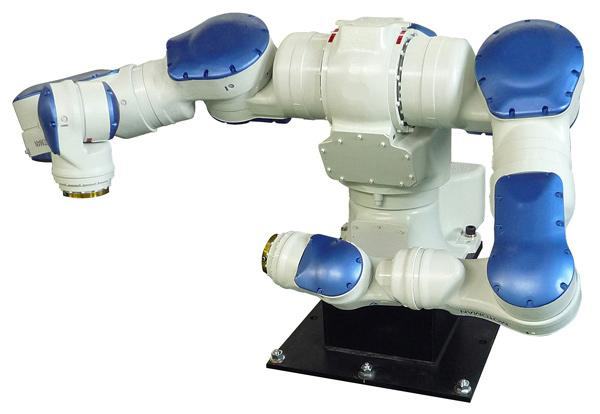
\includegraphics[scale=0.6]{FiguresSoA/TwoArms}\label{dosbrazos}}
\subfigure[Robot Kuka con 6 GDL]{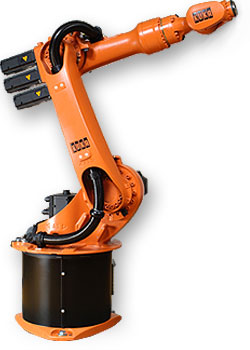
\includegraphics[scale=0.6]{FiguresSoA/KUKA}\label{kuka}}
\caption{Ejemplos de robots industriales}
\end{figure}




%The Motoman SDA5D assembly robot provides "human-like" flexibility in assembly applications. The Motoman SDA-5D DX100has two arms, 7 axes per arm, and one axis for base rotation. The arms can work together to double their payload capacity to 10kg (5kg per arm), which is the lowest payload in the SDA series, or they can work separately to accelerate assembly, part transfer, machine tending, packaging, or other handling applications. Cables and hoses are routed internally in the SDA-5D DX 100to reduce wear and simplify programming.


\section{Historia de la Teleoperación}
La teleoperación tal como la conocemos hoy en día tiene sus orígenes en los requerimientos de la industria nuclear \cite{goertz1952fundamentals}. Inicialmente se usaban pinzas de más de medio metro para separar al operador del material radioactivo, pero a medida que el trabajo con este tipo de material se iba haciendo mayor también aumentaba su  peligrosidad. Se emplearon pinzas con accionamiento remoto separando al operador del material mediante barreras de protección. El trabajo era bastante inc\'omodo debido a las restricciones de las pinzas por su paso por las barreras y la visión de la tarea se realizaba a través de espejos.\\


En 1947 en el Argonne National Laboratory de Estados Unidos se iniciaron las primeras investigaciones lideradas por Raymond Goertz, cuya finalidad era el desarrollo de sistemas de telemanipulación que facilitaran la realización de tareas remotas \cite{goertz1961manipulator}. En 1949 concluyó el desarrollo del primer manipulador teleoperado mecánico, llamado M1 \cite{goertz1952fundamentals},\cite{goertz1954mechanical}. \'Este podría ser considerado el antecesor de los sistemas de teleoperación maestro-esclavo existentes hoy en día. En los años posteriores continuaron los desarrollos basados en mejoras al M1, pero no fue sino hasta 1954 cuando Goertz presentó el primer manipulador maestro-esclavo bilateral con accionamientos eléctricos y servocontrolados, llamado E1.\\


A partir de 1956 Pesanti y Cherel comienzan a realizar un desarrollo de un sistema maestro-esclavo mecánico para la Agencia Atómica Francesa (\textsc{Commisariat de l’Energie Atomique}). Ese mismo año se desarroll\'o el sistema teleoperado Mascot, entre un equipo italiano y el \textsc{Argonne National Laboratory}. A finales de los años 50 se comenzó a aplicar esta tecnología al campo de las prótesis humanas y la rehabilitación en general.\\



En la figura \ref{Goertz} se muestra el telemanipulador de Raymond Goertz, fue un pionero en el campo de la robótica. Específicamente en el área de los robots operados a distancia (telepresecia). En 1951 mientras se encontraba trabajando para la comisión de energía atómica en \textsl{Argonne National Laboratory} desarrollo el primer manipulador de tipo maestro-esclavo con el propósito de manipular materiales radioactivos.


\begin{figure}[ht!]
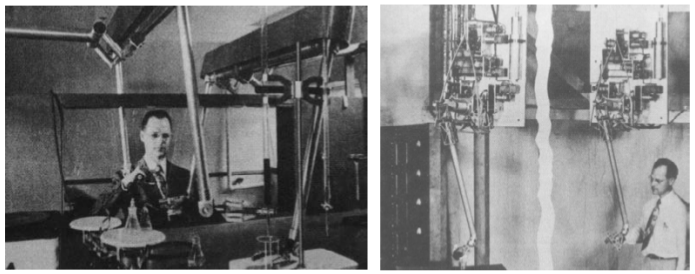
\includegraphics[scale=0.6]{FiguresSoA/Goertz}
\caption{El telemanipulador de Raymond Goertz años 50}
\label{Goertz}
\end{figure}


%La telerob\'otica es una \'area de la rob\'otica que concierne al control a distancia de sistemas rob\'oticos, generalmente a tr\'aves de comunicaci\'on inalambrica por ejemplo  wi-fi,  bluetooth,  radiofrecuencia dependiendo de la distancia o bien por redes de cominicaci\'on cableadas como  Ethernet   




%\begin{figure}
%\centering
%\subfigure[Robot K10 Rover]{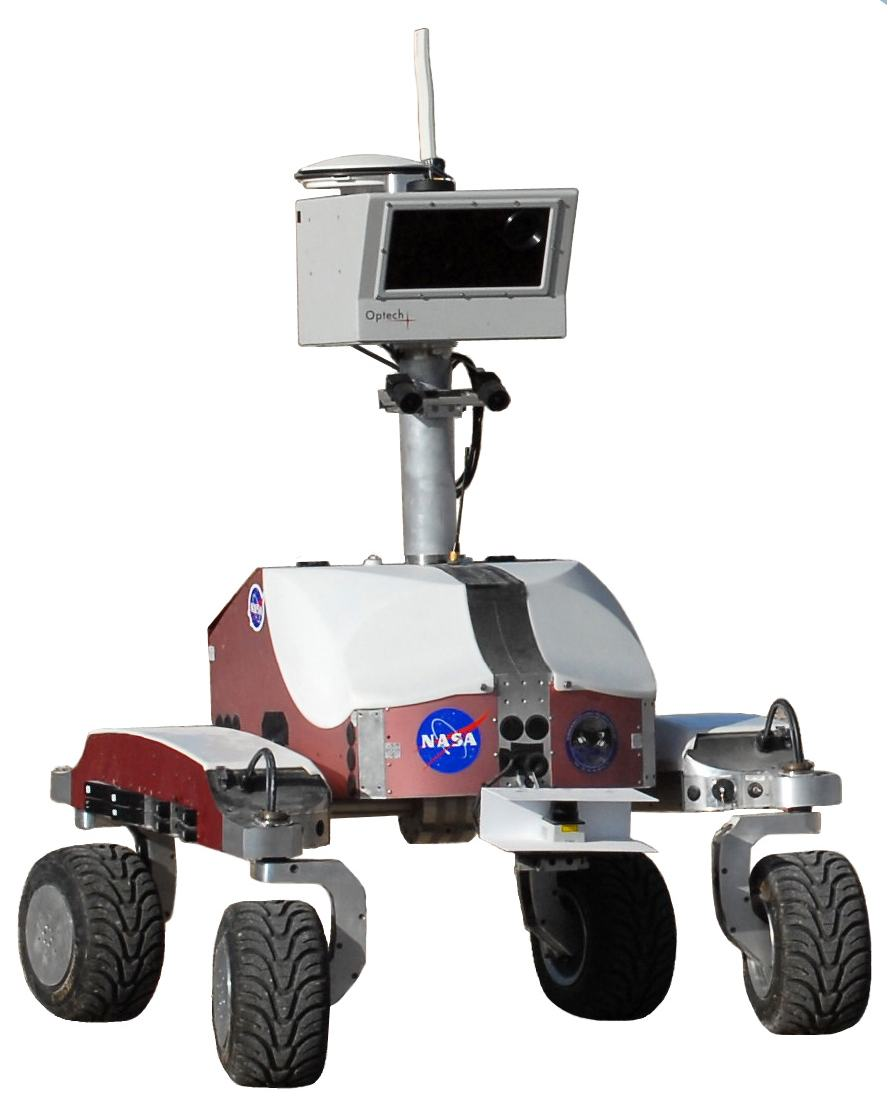
\includegraphics[scale=0.4]{Figures/K10Rover}}
%\subfigure[Retro excavadora controlada a trav{es de un maestro de Kraft Telerobotics]{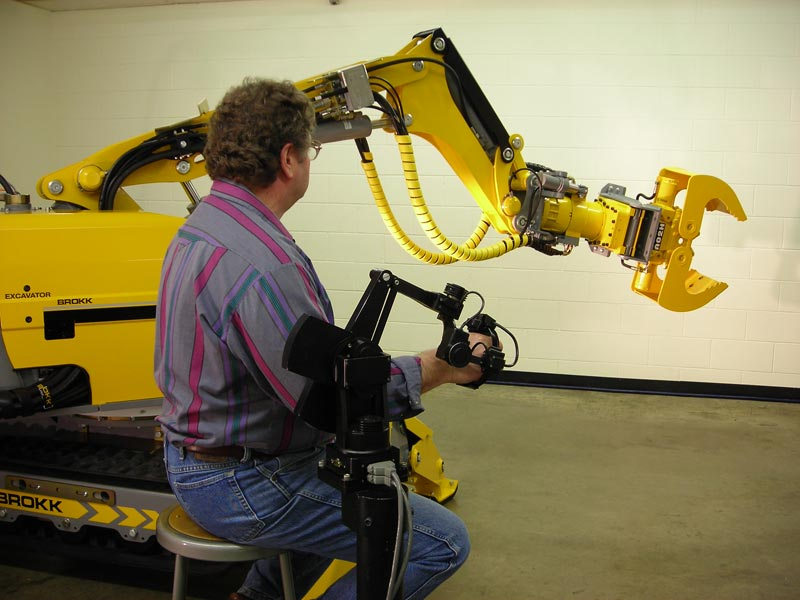
\includegraphics[scale=0.20]{Figures/retroExcavadora}}
%\caption{Ejemplos de robots teleoperados}
%\label{fig:teleoperados}
%\end{figure}




%Telerobotics is the area of robotics concerned with the control of robots from a distance, chiefly using wireless connections (like Wi-Fi, Bluetooth, the Deep Space Network, and similar), "tethered" connections, or the Internet. It is a combination of two major subfields, teleoperation and telepresence.

%Teleoperation

%eleoperation indicates operation of a machine at a distance. It is similar in meaning to the phrase "remote control" but is usually encountered in research, academic and technical environments. It is most commonly associated with robotics and mobile robots but can be applied to a whole range of circumstances in which a device or machine is operated by a person from a distance.[1]

%Teleoperation is standard term in use both in research and technical communities and is by far the most standard term for referring to operation at a distance. This is opposed to "telepresence" that is a less standard term and might refer to a whole range of existence or interaction that include a remote connotation.

%A telemanipulator (or teleoperator) is a device that is controlled remotely by a human operator. If such a device has the ability to perform autonomous work, it is called a telerobot. If the device is completely autonomous, it is called a robot. In simple cases the controlling operator's command actions correspond directly to actions in the device controlled, as for example in a radio controlled model aircraft or a tethered deep submergence vehicle. Where communications delays make direct control impractical (such as a remote planetary rover), or it is desired to reduce operator workload (as in a remotely controlled spy or attack aircraft), the device will not be controlled directly, instead being commanded to follow a specified path. At increasing levels of sophistication the device may operate somewhat independently in matters such as obstacle avoidance, also commonly employed in planetary rovers.

%Devices designed to allow the operator to control a robot at a distance is sometimes called telecheric robotics.

%Two major components of Telerobotics and Telepresence are the visual and control applications. A remote camera provides a visual representation of the view from the robot. Placing the robotic camera in a perspective that allows intuitive control is a recent technique that although based in Science Fiction (Robert A. Heinlein's Waldo 1942) has not been fruitful as the speed, resolution and bandwidth have only recently been adequate to the task of being able to control the robot camera in a meaningful way. Using a head mounted display, the control of the camera can be facilitated by tracking the head as shown in the figure below.

%This only works if the user feels comfortable with the latency of the system, the lag in the response to movements, and the visual representation. Any issues such as, inadequate resolution, latency of the video image, lag in the mechanical and computer processing of the movement and response, and optical distortion due to camera lens and head mounted display lenses, can cause the user 'simulator sickness' that is exacerbated by the lack of vestibular stimulation with visual representation of motion.

%Mismatch between the users motions such as registration errors, lag in movement response due to overfiltering, inadequate resolution for small movements, and slow speed can contribute to these problems.

%The same technology can control the robot, but then the eye–hand coordination issues become even more pervasive through the system, and user tension or frustration can make the system difficult to use.

%Ironically, the tendency to build robots has been to minimize the degrees of freedom because that reduces the control problems. Recent improvements in computers has shifted the emphasis to more degrees of freedom, allowing robotic devices that seem more intelligent and more human in their motions. This also allows more direct teleoperation as the user can control the robot with their own motions.

%Interfaces

%A telerobotic interface can be as simple as a common MMK (monitor-mouse-keyboard) interface. While this is not immersive, it is inexpensive. Telerobotics driven by internet connections are often of this type. A valuable modification to MMK is a joystick, which provides a more intuitive navigation scheme for planar robot movement.

%Dedicated telepresence setups utilize a head mounted display with either single or dual eye display, and an ergonomically matched interface with joystick and related button, slider, trigger controls.

%Future interfaces will merge fully immersive virtual reality interfaces and port real-time video instead of computer-generated images. Another example would be to use an omnidirectional treadmill with an immersive display system so that the robot is driven by the person walking or running. Additional modifications may include merged data displays such as Infrared thermal imaging, real-time threat assessment, or device schematics.




\section{Componentes de un sistema robótico teleoperado}


Una manera sencilla de describir un sistema teleoperado de robots es mediante un operador que envía instrucciones a un robot remoto, el cual ejecutará las órdenes correspondientes y enviará información de su estado y del entorno en el cual se encuentra. Esta información realimentada al operador será la que le permita cerrar el bucle de control del sistema teleoperado. Dentro de este ciclo existen otros elementos que intervienen y que son vitales para el funcionamiento del sistema, por lo que es necesario que sean tratados de manera individual. Para facilitar la identificación de todos los componentes de un sistema teleoperado, se va a hacer una división del sistema de acuerdo a su localización. En la figura , se puede observar que un sistema teleoperado básicamente puede ser dividido en tres partes: entorno local, entorno remoto y canal de comunicaciones.\\


\section*{Entorno Local}
En el entorno local se ubica el operador humano que es el encargado de controlar la ejecución de la tarea remota. Deberá contar con dispositivos de actuación que generen los comandos del operador para ser enviados al robot al entorno remoto. Para que el operador pueda tener conciencia del trabajo que está realizando se necesita dotar a la interfaz del sistema teleoperado de dispositivos de realimentación con los que el operador pueda tener información de la ejecución de la tarea. Dependiendo de la complejidad de la tarea y las condiciones de operación, puede ser necesario cerrar un bucle de control en la zona local, donde se presentan al operador ciertas ayudas que le faciliten la manipulación, bien sea para mejorar su desempeño o para superar adversidades propias a la aplicación como por ejemplo los retardos en la comunicación.




\subsection*{Operador}
El operador es la persona encargada de realizar la tarea y el elemento que cierra el bucle de control. Su intervención puede ser diversa, dependiendo de la aplicación y puede ir desde un control absoluto, pasando por un control compartido hasta otro supervisado.




\subsection*{Dispositivos de actuación}
Son los dispositivos encargados de capturar los comandos generados por el operador para ser transmitidos al manipulador remoto. Existe una gran variedad de dispositivos capaces de realizar esta función, cada uno con características propias, ventajas y desventajas. Entre los más comunes podemos nombrar: teclados, ratones, joysticks, dispositivos maestros, dispositivos maestros con reflexión de fuerza, paletas, pantallas táctiles, pedales, etc. Los joysticks generan habitualmente comandos de velocidad, mientras que los maestros generan comandos de posición, aunque también puede ser programado para generar comandos de velocidad. Es posible hacer uso de otro tipo de dispositivos, simplemente cambiando el medio a través del cual se emiten los comandos, por ejemplo micrófonos para comandos de voz, cámaras para sistemas de captura de movimiento. Un estudio más detallado de los mismos puede ser encontrado en \cite{Ferre2007a}.


\subsection*{Dispositivos de realimentación}
Son los dispositivos encargados de presentarle al operador cualquier tipo de información relacionada con el desarrollo de la tarea que está realizando. Un operador no puede realizar una operación si no puede ver qu\'e es lo que está haciendo. Como en la actualidad prácticamente en todas las aplicaciones teleoperadas el entorno local se encuentra físicamente separad del entorno remoto, el dispositivo de salida indispensable en cualquier operación es el TV o monitor a través del cual se le presentará al operador imágenes de la tarea. Los monitores también son capaces de presentarle al operador información de tipo textual, gráfica o  de imágenes compuestas entre realidad y simulación. Existen maestros y joysticks con reflexión de fuerzas que son capaces de presentarle al operador fuerzas de contacto y manipulación relacionadas con la tarea ejecutada, ademas de cumplir la función de dispositivo de entrada. También es posible hacer uso de altavoces para emitir sonidos, alarmas o información auditiva al operador.


\section*{Entorno remoto}
Es el entorno en el que se encuentra ubicado el robot esclavo y se llevan a cabo la tarea. Es importante resaltar que a diferencia del robot industrial, el entorno de trabajo de un robot usado como manipulador teleoperado, es por lo general, no estructurado, variable o desconocido. Debido a que el operador humano es el que cierra el bucle de control del manipulador esclavo, \'este no requiere de gran precisión en sus movimientos (siempre y cuando el error no sea acumulativo) ya que el operador realizará las correcciones necesarias.



\section*{Canal de comunicaciones}
A través del canal de comunicaciones fluye la información desde el entorno remoto hacia el entorno local y viceversa. Pueden usarse distintos métodos o distintos dispositivos como canal de comunicaciones, la transmisión de información puede llevarse a cabo por medio de cables o sin ellos, las características principales para elegir un canal de comunicaciones suelen ser el ancho de banda, retardos temporales y la robustez de los protocolos de comunicación. Algunos ejemplos pueden ser Internet, redes de fibra óptica, comunicación Serie RS-232, USB, radio frecuencia, entre otras, aunque también depende de la distancia que se tenga entre el entorno remoto y el entorno local. Por un lado el ancho de banda se refiere a la cantidad de información que el canal es capaz de transmitir, mientras que el retardo temporal lo determina el tiempo que tarda la información en ir desde una zona a la otra.


 

%\section*{Modelado de los Elementos del Sistema Robótico Teleoperado}
%Para realizar el estudio de los distintos esquemas, generalmente pueden utilizarse dos métodos de modelado: el método de \textsc{Euler-Lagrange} por medio de la energía del sistema, o bién por el método de \textsc{Newtom-Euler} por medio de las ecuaciones de la cinemática Las ventajas de utilizar el Método de energías de \textsc{Euler-Lagrange} son: que tenemos las ecuaciones resumidas en una forma más compacta involucrando también las matrices de coriolis y la posibilidad de modelar eslabones deformables con su energía de deformación. 


%\section*{Modelado del Operador}
%aquí falta lo del modelado tipo kelvin y todo eso


%\section*{Modelado del Entorno}



%\section*{Algoritmos de Control Bilateral}

%Es la principal área de investigación desde los inicios de la teleoperación, con lo cual es bastante extenso el material referente a este tema. Existen diversos esquemas aplicando control clásico, moderno, teoría de cuadripolos, variables de ondas, etc. No se detallarán esos esquemas porque en la presente tesis existen otros capítulos dedicados a estos temas donde serán tratados con mayor profundidad, simplemente se mencionarán algunos de los desarrollos que diversos investigadores han implementado en la actualidad. Vale la pena resaltar que en lo que a control se refiere un tema que se encuentra en pleno desarrollo es el del control con retardos en las comunicaciones, impulsado inicialmente por su aplicación el sector espacial y submarino, y especialmente motivado en la actualidad por la implementación de sistemas haciendo uso de Internet como medio de comunicación. En el trabajo realizado en [Richard 03], se hace un resumen de los principales modelos usados para describir el retardo temporal, algunos de los esquemas de control usados y problemas abiertos en este campo como por ejemplo: la implementación de los sistemas con retardo temporal de manera digital, identificación adaptativa del retardo, captura y manejo de información relacionada con el retardo, uso de las propiedades estocásticas del retardo. Otro trabajo como el presentado por Blake Hannaford [Hannaford 02], se muestra un método basado en la energía, controlando una interfaz háptica para asegurar un contacto estable bajo una gran variedad de condiciones de operación, como el contacto con entornos de gran rigidez, limitando la fuerza de control y entorno con retardos. Se analiza la estabilidad del sistema en términos de la definición de la pasividad en el dominio del tiempo. Se define el Observador de Pasividad que mide el flujo de energía entrante y saliente de uno o más subsistemas en tiempo real.\\
 


%Un comportamiento activo se verifica con un valor negativo del Observador de Pasividad en cualquier momento. También se define el Controlador Pasivo, un elemento adaptativo disipante, que en cada tiempo de muestreo, absorbe exactamente la salida de energía neta (en caso de haberla) medida por el Observador de Pasividad. Existe un esquema de control bilateral basado en la realimentación hacia adelante (Feedforward) para telemanipuladores lineales dinámicamente parecidos, con escalado cinestésico y de potencia, el mismo se puede encontrar en [Lee 03]. La ley de control propuesta, modela al operador como una herramienta mecánica rígida pasiva con inercia aparente programable parecida al operador humano y al entorno de trabajo remoto, utilizando Feedforward bilateral de fuerza y control con realimentación de posición. La pasividad del sistema de lazo cerrado es robusta ante imprecisiones en las medidas de fuerzas y errores de modelado. La coordinación de errores y aspectos generales de movimiento de la teleoperación son controladas individualmente. El esquema propuesto es aplicable a sistemas generales teleoperados no lineales si se garantiza el uso de una alta ganancia de realimentación. Existen otros trabajos cuyo objetivo es el estudio de ciertas condiciones de funcionamiento como por ejemplo el retardo en las comunicaciones, en este sentido, [Niculescu 02] realiza un análisis de la estabilidad de un esquema de control de teleoperación a lazo cerrado ante la presencia de retardos en la comunicación. Derivando condiciones de estabilidad en el dominio de la frecuencia analíticas y fáciles de verificar. 


%Se estudian casos de independencia del retardo así como intervalos de retardos. La novedad de este trabajo radica en la simplicidad de la caracterización de regiones de estabilidad en términos de los parámetros del sistema. Se presentan tanto interpretaciones físicas como diversos ejemplos. Otra metodología de control que se ha empleado es el control combinado de posición/fuerza de sistemas de telepresencia con reflexión de fuerza y retardos en la comunicación como el desarrollado en [Hirche 03]. Presentando un método de diseño de filtros por igualación de impedancias con optimización en el dominio de la frecuencia con la finalidad de conseguir la pasividad en el Operador/Entorno y transparencia en el sistema de telepresencia controlado en posición/Fuerza. De igual manera en un trabajo presentado en [Leeraphan 02] se muestra una metodología muy similar solo que la igualación de la impedancia se realiza de manera adaptativa con el tiempo. Existen estudios detallados del uso, análisis y diseño de sistemas telemanipulados con variables de onda, los mismos se basan en el concepto de la potencia y la energía, como por ejemplo [Niemeyer 04], donde se presenta una modificación o extensión de la teoría de la pasividad, creando robustez ante retardos temporales arbitrarios. En este estudio se muestra que el uso de las variables de ondas ofrecen diversos beneficios como:

%Robustez ante retardos temporales de varias magnitudes, para retardos nulos el sistema se revierte automáticamente a una configuración de teleoperación clásica. Para retardos pequeños, el sistema se mantiene robusto y estable. La impedancia de la onda, o matriz de impedancia, provee un mecanismo de ajuste on-line, permitiendo al usuario configurarlo para movimientos rápidos, o reflexión de fuerza sensitiva, dependiendo de la tarea. Mediante el uso de las integrales de onda, el sistema puede combinar toda la información relevante, por ejemplo: posición, velocidad, aceleración, fuerza, en una simple cantidad, reduciendo los requerimientos de transmisión. Vale la pena resaltar que aplicando esta filosofía, los autores efectuaron la teleoperación de un robot con un retardo constante de 2 segundos, así como también retardos variables a través de Internet de 50 mSeg a 1 Segundo. Otro trabajo relacionado con el uso de las variables de onda es el presentado en [Munir 02], donde se realiza un estudio usando las variables de ondas, pero en este caso el grueso del desarrollo se centra en la incorporación de un predictor de Smith, un filtro de Kalman y un regulador de energía al esquema con la finalidad de mejorar la estabilidad del sistema. El predictor no necesita conocer las condiciones iniciales, y el filtro de Kalman eventualmente convergerá al estado interno correcto del esclavo visto desde el lado de la comunicación del maestro. Ya que el estado del esclavo se ve afectado directamente por su interacción con el entorno, y el predictor depende del filtro del Kalman para estimar el estado interno del esclavo, no se necesita medir las fuerzas ejercidas por el entorno al maestro. Se muestra que el sistema es estable aún en la presencia de incertidumbre en el modelo del sistema remoto. Otro trabajo relacionado con el uso del predictor de Smith, puede encontrarse en [Ganjefar 03], donde se presenta un estudio del comportamiento de un sistema de teleoperación con errores de modelado y de retardo de comunicación con el uso del predictor\cite{welch1995introduction}.\\
 
 

%Se presenta unas condiciones de estabilidad para el caso de los errores de modelado, que sirve de ayuda a los diseñadores para asegurar la estabilidad del sistema. También se realiza un estudio del efecto de la predicción del retardo en la estabilidad y se demuestra que dicha predicción puede mejorar el desempeño del sistema. Existen otros trabajos cuya finalidad es la de obtener nuevos esquemas, como por ejemplo [Ryu 04], donde se presenta un nuevo esquema de control basado en el concepto de la pasividad, con la finalidad de garantizar la estabilidad de la teleoperación ante una gran variedad de entornos y velocidades de operación. Se ha extendido un método basado en la energía de una red de 1 puerto a una red de 2 puertos, estudiando la implementación de un observador y un controlador de pasividad. El controlador desarrollado no mejora el desempeño (transparencia), sino preserva el desempeño garantizando la estabilidad, para un sistema de gran desempeño, mediante la inclusión de un observador y un controlador de pasividad a un esquema bilateral convencional. Con relación al tema de la transparencia en la teleoperación con retardos en las comunicaciones, en [Zaad 02] se estudia las ventajas de emplear la reflexión de fuerza local, para mejorar la estabilidad y el desempeño. Se presentan 2 esquemas de control de 3 canales, 1) Arquitectura de compensación de fuerzas por el operador y 2) Arquitectura de compensación de fuerzas por el entorno, ambas son perfectamente estables bajo condiciones ideales, y se analiza su estabilidad rigurosamente ante la presencia de retardos. Existen desarrollos de nuevas metodologías de reflexión de fuerzas, como puede observarse en [Love 04], donde se reducen los requerimientos de energía por parte del operador sin sacrificar la estabilidad, el autor explica que la estabilidad en los sistemas de teleoperación con reflexión de fuerzas requiere altos niveles de amortiguamiento, lo que a su vez incrementa los requerimientos de energía por parte del operador. Se realiza una aproximación novedosa de modelado e identificación del entorno remoto, combinando la identificación recursiva convencional de múltiples entradas y múltiples salidas de mínimos cuadrados, identificando en tiempo real la impedancia del entorno con un modelo discretizado del entorno. Esta metodología genera una representación de la dinámica del entorno variante en el tiempo, dependiente de la posición. Seguido a la estimación del entorno, se adapta la impedancia del robot maestro, respecto al modelo dinámico del entorno. Tanto la estimación del entorno como la adaptación de la impedancia se realizan simultáneamente y en tiempo real. Se demuestra prácticamente, mediante experimentación que esta metodología disminuye lo requerimientos de energía por parte del operador, mientras que se provee de suficiente amortiguación para asegurar la estabilidad en el contacto. Otras investigaciones estudian aspectos como por ejemplo, la relación entre los parámetros de impedancia y factor de escalado derivados del uso del concepto de máxima estabilidad y pasividad, como puede encontrarse en [Cho 02]. En la actualidad aún existen investigaciones de interés basadas en los esquemas bilaterales de control clásico, por ejemplo en [Ni 02] donde se desarrolla un esquema de control posición-posición basado en la adaptación de ganancia, con la finalidad de reducir el costo de los sistemas de teleoperación evitando el uso de sensores fuerza/par que ofrece una transparencia pobre. El mismo se basa en la detección de los cambios de impedancia en el lado del esclavo, luego las ganancias de los controladores del maestro y del esclavo son cambiadas en consecuencia. Se presentan resultados experimentales para demostrar la efectividad de este esquema.\\

%Finalmente, en [Benedetti 01] se describe una arquitectura mejorada para el control de la teleoperación con reflexión de fuerzas, en presencia de retardos en las comunicaciones entre maestro y esclavo, está basada en la transformación de variables de onda y la identificación de las propiedades del retardo. Este esquema consigue mejor desempeño en el seguimiento de posición y fuerza que otros esquemas similares, mediante la estimación del valor actual del retardo y compensando sus variaciones ajustando un parámetro de control. También se derivan algunas propiedades analíticas de dicho esquema y demuestra el desempeño del esquema simulando un sistema teleoperado.


\section{Interfaces Hombre-Máquina}
Las interfaces hombre m\'aquina (del ingl\'es \textsc{Human-Machine Interface HMI})de un sistema teleoperado son el puente que une al operador con el entorno de trabajo. Como se mencionó anteriormente, está compuesta por los dispositivos de entrada, dispositivos de salida y el control en zonal local. Debe ser sencilla de manejar, robusta, completa y sobre todo facilitar al operador la realización de las tareas remotas. En \cite{Ferre2007a}, se identifican tres puntos que debe cumplir una interfaz, a saber:

\begin{enumerate}
\item  Establecer todas las conexiones necesarias entre el operador y la zona remota de trabajo. Se dan dos tipos de conexiones: las de actuación del operador sobre el entorno remoto y, en sentido contrario, las de realimentación de información hacia el operador.

\item Facilitar la ejecución de tareas permitiendo al operador enviar comandos de alto nivel referentes al trabajo a realizar, a la vez que posibilite su actuación directa cuando sea preciso.

\item Suministrar al operador toda la información necesaria del entorno de trabajo con el fin de que alcance el mayor grado posible de transparencia. Esto le permitirá ejecutar tareas con destreza, así como facilitarle la supervisión de las tareas semiautomáticas.

\end{enumerate}

Debido a la  función vital que cumple la interfaz dentro del sistema teleoperado, se realizan gran cantidad de desarrollos e investigaciones con la finalidad de aumentar cada día más sus capacidades.\\

% Entre los principales puntos en los cuales se enfocan las investigaciones en la actualidad tenemos:\\


%Estudio del desempeño de las Interfaces: Cuando se desarrolla la interfaz de un sistema teleoperado, para poder llegar a alguna conclusión de su desempeño, no solo se tiene que evaluar por su comportamiento técnico como tal, sino al ser la conexión entre el entorno remoto y el operador, es necesario evaluar también su relación con el operador, ya que aún cuando una interfaz técnicamente sea perfecta si los operadores no pueden manejarla por su complejidad, o porque les sea muy incomoda, no se puede implementar en una aplicación real. Por ello es que se han realizado investigaciones en cuanto a la manera de evaluar el desempeño de las interfaces. Existen numerosos estudios de como determinar lo que denomina Calidad de la Experiencia, que es la relación que mantuvo la interfaz con el operador durante la realización de la tarea.Para estudiar esa relación se proponen 3 métodos de recolección de información:\\


%\begin{enumerate}
%\item Medidas Sujetivas: Se obtienen preguntando directamente al usuario como se siente. Estas preguntas pueden ser mediante cuestionario o entrevista y también se pueden clasificar: a) De hecho: son las preguntas que recogen información
%como la edad, años de experiencia con computadores, nivel de educación. B) Tipo opinión: Se refiere a los pensamientos del interrogando acerca de estímulos externos, otras personas u objetos. C) Preguntas de actitud: Se refieren a las
%respuestas internas del interrogando respecto a eventos y situaciones relacionadas con un producto en particular.
%
%\item Medidas de Desempeño: Son medidas prácticas, menos propensas a errores que los cuestionarios. Las medidas pueden ser la cantidad de errores cometidos, tiempo de ejecución, precisión en las operaciones, etc.
%\item Medidas fisiológicas: Son medidas como el estrés, la actividad cerebral, la cyber-enfermedad.
%\end{enumerate}
%
%Las medidas que pueden reflejar la cyber-enfermedad son: el ritmo cardíaco. Niveles de cortisona en la saliva y estabilidad postural. En ese estudio se concluye que una buena calidad de la experiencia se obtiene maximizando 3 dimensiones:\\
%
%\begin{enumerate}
%\item  El disfrute de la experiencia por el operador.
%\item  Su habilidad de lograr sus objetivos.
%\item  La menor cantidad práctica de estrés e incomodidad.
%\end{enumerate}
%
%A la hora de que un investigador tenga que escoger un instrumento para medir cualquiera de esas dimensiones debe escoger el mejor instrumento, a manera general propone:\\
%
%\begin{enumerate}
%\item  Para el disfrute de la experiencia, como estado interno del usuario, se mide mejor con un instrumento sujetivo, como un cuestionario o entrevista.
%\item El proceso hacia el objetivo, el comportamiento del usuario, generalmente se miden mejor con una observación del comportamiento.
%\item  El estrés, incomodidad, son medidas que se miden con instrumentos fisiológicos.
%\end{enumerate}
%
%Reflexión multisensorial: Debido a la perdida de la información sensorial que ocurre por efectos de la teleoperación, se recurre a lo que se denomina sustitución sensorial, que no es otra cosa que inducir o provocar sensaciones artificiales al operador que estén controladas o generadas mediante la aplicación de las leyes físicas que rigen los movimientos o esfuerzos que se realizan para completar la tarea. Esta sustitución sensorial depende en si de la naturaleza del sentido que se quiera sustituir, por ejemplo: en el caso de la vista, debido a que el operador y el esclavo se encuentran en entornos distintos, se presenta bien sea mediante el uso de un monitor dedicado o una ventana imágenes correspondientes a la tarea que realiza el esclavo. Aparte si se quiere dar la sensación de profundidad que se pierde, se hace uso de técnicas 3D, cámaras estereo. En el caso del oído, bastaría simplemente mediante el uso de micrófonos y parlantes llevar
%al operador los sonidos que se generan en el entorno de trabajo (si la tarea lo requiere). Otra manera es hacer uso de señales sonoras como alarmas o avisos relacionados con la tarea que se esta realizando. Una de las técnicas que más se usa para la sustitución de este sentido es el uso del los maestros con reflexión de fuerza, que no hacen otra cosa que reflejar los esfuerzos que realiza el esclavo en el maestro.\\
%
%En este sentido, en \cite{Ferre2007} se realiza un estudio sobre la reflexión de fuerzas usando métodos gráficos (visual), auditivos (sonidos) y cinestésicos (tacto). Donde se concluye que el uso de la realimentación cinestésica de fuerzas es la mejor forma de presentarle al operador una aproximación de la fuerza ejercida y combinada con una realimentación visual o auditiva realzan la información percibida por el operador, mientras que la combinación de las 3 no mejora la percepción respecto a la obtenida por la combinación de la realimentación cinestésica con la auditiva o visual. En [Williams 02], se hace un estudio de la combinación de la realimentación cinestésica con la visual, donde se muestra una mejora significativa en el desempeño de una tarea, indicada por una reducción de la varianza entre 61\% y 90\% en las fuerzas de contacto, reducción de pares entre 46\% y 92\% usando cualquier medio de reflexión de fuerzas. Y mediante el uso de ambos tipos de reflexión simultáneamente presentaba mejores desempeños.\\
%
%Interfases Multimodales: Este es un tema que ha incrementado su interés entre los investigadores. Una interfaz multimodal es aquella en la cual se le presenta al operador un flujo continuo de información en distintas modalidades de la percepción humana, cinestésica, táctil, visual, auditiva, todo con la finalidad de aumentar el grado de inmersión del operador con la tarea que esta realizando. Muchas de las investigaciones se centran el desarrollo del hardware, en \cite{aleotti2002multimodal} se desarrolla una interfaz multimodal concebida para la teleexploración de entornos remotos, la misma cuenta con realimentación de video, simulador 3D, realimentación vibrotáctil y es manejada usando un guante cybertouch de Inmersion Corp. Inc. En \cite{preusche2002teleoperation}, se desarrolla un sistema de telepresencia multimodal a través de Internet que incluye realimentación visual, auditiva, cinestésica y display predictivo, logrando un gran nivel de inmersión en la manipulación con el entorno remoto.





\subsection{Interfaces Hápticas}
Háptica se refiere al sentido del tacto del mismo modo que óptica se refiere al sentido de la vista o acústica al sentido del oído. De modo que las interfaces hápticas son las que permiten que una computadora se comunique con nosotros a través del tacto, generalmente para darnos una realimentación táctil de alguna interacción. Podemos dividir estas realimentaciones en dos categorías según la información táctil que se pretende replicar: realimentación táctil y realimentación cinestética. La primera proporciona información al usuario a través de las terminaciones nerviosas de la piel dando información sobre textura, geometría o temperatura. La segunda ofrece información sobre la posición y movimiento de la mano, de modo que se obtenga una información de las fuerzas que se están ejerciendo (o del peso de un objeto si se está sujetando) y de la elasticidad o rigidez de lo que se está tocando. Es común hablar de realimentación de fuerza para describir la realimentación táctil y/o la realimentación cinestética.

Las interfaces hápticas permiten simular interacciones con objetos reales, que pueden ser útiles para telepresencia  o teleoperación, sintiendo de ese modo a distancia las fuerzas que se están ejerciendo sobre un objeto, pudiendo por ejemplo sentir la presencia de otra persona tocando un objeto a distancia o teleoperar varios aviones no tripulados \cite{troy2011systems,stigter2007design}. También se utilizan para experimentar la interacción con objetos virtuales, algo muy útil para el entrenamiento, existiendo por ejemplo investigaciones que han terminado como tecnologías comerciales para la capacitación en cirugía \cite{sun}. La tecnología háptica, con un nivel de realismo todavía muy limitado, también está presente en la industria del videojuego.

Existen muy diversas tecnologías y prototipos para la implementación de interfaces hápticas. El desarrollo de estas tecnologías permitirá en combinación con otras tecnologías la implementación de interfaces más naturales, como por ejemplo pantallas táctiles que proporcionen realimentación háptica  de modo que se pueda interactuar con un teclado virtual de forma parecida a  un teclado físico, es decir, sin mirar constantemente el mismo.


Las primeras interfaces hápticas fueron desarrolladas  para el control de servo-mecanismos en grandes aviones con la intención de operarlos a distancia. Estos primeros sistemas  operaban en una única vía de tal forma que la fuerza aplicada en la palanca de control se multiplicaba en las superficies de control aerodinámico (alerones, motores, turbinas, entre otras), pero el piloto no tenía una percepción de la fuerza que estaba siendo aplicada realmente \cite{abel2010pilot,abel2007pilot}. En los inicios de la aviación los pilotos de aviones pequeños sin servo-mecanismos tenían todas las sensaciones acerca de la resistencia del aire en los alerones esto suponía una seguridad en ciertas situaciones de peligro. Con la aparición de los primeros servos, el piloto no obtenía esta sensación. Para resolver este problema se instaló un sistema de control que proporcionaba una resistencia a la  palanca del piloto proporcional al ángulo de ataque de los alerones \cite{troy2011systems,stigter2007design,hanlon2011active}.\\


Por otro lado, los teleoperadores y simuladores que controlaban máquinas y herramientas a distancia  en los cuales el usuario era capaz de sentir las fuerzas aplicadas establecieron un precedente en la investigación de interfaces hápticas. A esto se le denominó teleoperación háptica. Despues del primer  teleoperador háptico desarrollado Goertz en 1950 \cite{goertz1961manipulator,goertz1954electrical,goertz1954mechanical,goertz1952fundamentals}. La realimentaci\'on en fuerza ha sido empleada en muchos tipos de teleoperación como en la exploración de las profundidades marinas \cite{domingues2012human}.\\



Los simuladores hápticos se usan en la actualidad para el entrenamiento de los estudiantes de medicina que pueden ser futuros cirujanos, evitando la necesidad de practicar con pacientes reales \cite{sun,waldron}. También son muy usuales los simuladores de vuelo  para el entrenamiento de los pilotos, los cuales son indispensables hoy en día, ya que gracias a estos se evitan catástrofes aéreas, ayudando a los jóvenes pilotos a obtener experiencia sin necesidad de poner en riesgo sus vidas y reduciendo los costes de este entrenamiento \cite{lam1983flight}.\\ 


A partir de la Primera Guerra Mundial fueron desarrollados  vehículos aéreos no tripulados UAV por sus siglas en inglés (\textsl{Unmanned Aerial Vehicle}), también conocidos por sus siglas en español como VANT, dotados de un sistema de control con realimentacion háptica en los controles de vuelo. Estas aeronaves son usualmente preferidas para tareas que resultan peligrosas para los aviones tripulados \cite{chandler2000uav}. Aunque actualmente estas aeronaves son operadas de forma totalmente autónoma pues el piloto u operador únicamente tiene que fijar las coordenadas de destino en el mapa y el sistema de control de vuelo se encarga de dirigir la aeronave a su destino. En este caso la única tarea del piloto es manejar las cámaras de largo alcance para poder enfocar el objetivo, ya sea para cuestiones de espionaje, seguridad, o marcar las coordenadas donde debe de impactar una bomba o un misil. Es importante destacar que el operador puede tomar control manual sobre la aeronave en caso de emergencia \cite{nikolos2003evolutionary}.\\



La realimentación háptica es comúnmente usada en vídeo juegos. En 1976 el juego de motocicletas \textsl{Moto-Cross}  también conocido como \textsl{Fonz} desarrollado por la compañía \textsl{Sega\textregistered}, fue el primer juego en proporcionar una realimentación de fuerza, la cual se manifestaba al momento de una colisión mediante la vibración de un volante de motocicleta ubicado en la parte superior de la consola \cite{wolf2008video}. Dispositivos hápticos simples usados en la mayoría de los vídeojuegos actuales pueden ser controles, joysticks y volantes de automóvil, los cuales permiten al usuario una realimentación por medio de vibraciones.  La forma más sencilla de proporcionar una sensación háptica en un juego es la vibración en los controles, con la que el usuario puede experimentar algunas irregularidades tales como golpes en un juego de peleas, disparos en un juego de combate o un choque en un juego de carreras de autos \cite{chang2002haptics}.\\



\begin{figure}[htb!]
\centering
\subfigure[Two Phantoms]{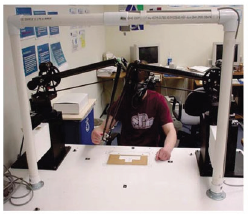
\includegraphics[scale=0.90]  {FiguresSoA/TwoPhamtoms}\label{fig:twophamtoms}}
\subfigure[Cyber Grasp ]{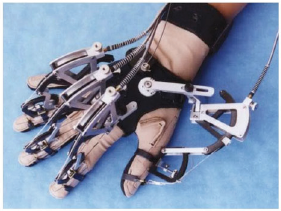
\includegraphics[scale=0.90]{FiguresSoA/CyberGrasp}\label{fig:cybergrasp}}
\subfigure[Spydar]{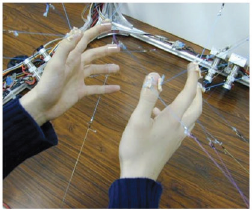
\includegraphics[scale=0.90]{FiguresSoA/Spydar}\label{fig:spydar}}
\subfigure[Hiro III]{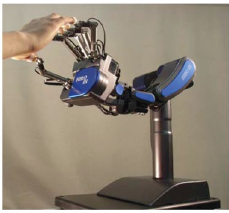
\includegraphics[scale=0.90]{FiguresSoA/hiro3}\label{fig:hiro3}}
%\label{fig1}
\caption{Ejemplo de algunas interfaces hápticas}
\end{figure}

%\cite{Kawasaki,endo2008fpga,endo2011multi,kawasaki2003control,kawasaki2006haptic,kawasaki2007design}
Ejemplos de dispositivos hápticos más parecidas al trabajo que se pretende realizar son: Two Phantoms, CyberGrasp, Spydar y HiroIII, Ver figura 1.  Las interfaces hápticas multidedo antes mencionadas están basadas en el uso de varios dispositivos hápticos de un solo dedo. Algunas toman lecturas de la  posición de la mano humana, para poder aplicar una fuerza en una mano robótica humanoide y tomando datos de sensores en la mano robótica, permitiendo la interacción bidireccional. Otras utilizan la información de la mano humana para producir una interacción con un entorno virtual.\\

 Uno de los dispositivos hápticos de un solo dedo más populares es Phantom de SensAble Tecnologies ver figura \ref{fig:twophamtoms}. \'Este ofrece una solución simple que se basa en una alta precisión en el efector final, mediante la fijación de un punto en el espacio de trabajo por cada dedo. El problema principal de esta configuración radica en las colisiones entre los eslabones del dispositivo que se traduce en una disminución del área de trabajo.\\


Por otro lado han sido desarrollados dispositivos que incluyen varios puntos de contacto y además pueden ser utilizados en varias aplicaciones para ofrecer una mayor destreza de manipulación. Estas soluciones ofrecen un mejor rendimiento en cuanto manipulación y un aumento significativo en el área de trabajo.\\ 

La figura \ref{fig:cybergrasp} muestra el prototipo CyberGrasp que consta de un exoesqueleto que permite el control individual de cada uno de los cinco dedos. Este dispositivo únicamente puede reflejar fuerzas normales en las puntas de los dedos, sin ninguna componente tangencial, y por lo tanto el usuario puede penetrar un objeto tangencialmente sin ninguna realimentación de fuerza. Con este dispositivo es necesario un punto de referencia fijo en la muñeca para poder calcular su localización 3D.\\

 La figura \ref{fig:spydar} muestra un dispositivo háptico basado en una estructura paralela de cables llamado Spydar \cite{lopez2012mechanical}. La versión actual implementa puntos de contacto para todos los dedos. Como se puede observar este tipo de configuración es más eficiente en cuanto a la precisión pero su espacio de trabajo est\'a restringido para evitar que se enreden los cables. Esto limita en gran medida las tareas cooperativas o que involucran el uso de ambas manos. Por otro lado, soluciones más complejas como el robot háptico Hiro III\cite{Kawasaki,endo2008fpga,endo2011multi,kawasaki2003control,kawasakiforce,kawasaki2007design,mouri2005developments,mouri2006novel} también proveen puntos de contacto en todos los dedos. Sin embargo es demasiado sofisticado y requiere del multiples sensores de fuerza/par (uno por cada dedo), lo cual incrementa su costo significativamente.\\
 
  La figura \ref{fig:hiro3} muestra la configuración especular del robot Hiro III. Como Spydar ésta configuración puede presentar inconvenientes cuando se realizan tareas bimanuales debido al limitado espacio de trabajo disponible. 



\subsection{Interfaces Visuales}

La realimentación visual es de vital importancia en las interfaces de teleoperación, ya que si el operador no puede ver lo que esta haciendo no puede realizar ninguna tarea. Es por esto, que muchas investigaciones realizadas buscan mejorar la calidad de la realimentación visual del operador. La mejora en la calidad de la realimentación estéreo es un punto donde se realizan grandes esfuerzos, porque la percepción de profundidad en teleoperación es vital para el buen desempeño del operador. 

%Por ejemplo, en [Hopf 00], se realiza un diseño de un sistema estereoscópico adaptativo basándose en la aplicación de espejos esféricos y óptica colimada, el mismo presenta un alto grado de telepresencia, además mejora las condiciones de visión del operador, permitiéndole trabajar por tiempos mas prolongados. En el centro de investigación Langley de la NASA, también se han realizado investigaciones al respecto, por ejemplo en [Parrish 95], se mostró que el volumen de profundidad disponible se incrementa con el uso de óptica colimada. En [Runde 00], desarrollan un sistema estereoscópico con paralaje de movimiento para la captura y reproducción de imágenes estereo. En el mismo, no se usan dispositivos como gafas esteros o cascos estereos, ya que consideran que de esa manera la sensación es más natural. En [Mulligan 01], se realiza un estudio del desempeño de los algoritmos de generación de imágenes estereo para la telepresencia. En [Adelstein 00], por otro lado, se estudia los efectos de agregar un grado de libertad, el de roll a las plataformas de cámaras de telepresencia al conocimiento espacial del operador. En [Ferre 03], se presenta el diseño de una cámara estereo novedosa, donde la imagen es insertada directamente en la comunicación VGA entre el ordenador y el monitor, evitando consumir recursos del sistema que pueden ser usados en otras tareas, además de la generación de imágenes estereo también tiene la capacidad de efectuar blending, es decir la superposición de imágenes reales con imágenes simuladas. Otras de las líneas de investigación con el uso de la visión es su aplicación no como medio de realimentación al operador, sino como dispositivo de entrada de los sistemas teleoperados. En [Colombo 01], se realiza un estudio de un sistema de captura y reproducción de posturas del cuerpo humano usando modelos computarizados. En [Maaoui 01], se implementa un sistema de las mismas características pero aplicado a un sistema teleoperado. El desafío en estas aplicaciones radica en el cálculo en tiempo real de la posición del operador y su mano, así como su configuración. Para poder emitir comandos de posición o movimiento de una manera más natural, mediante el uso de gestos con las manos o con el cuerpo entero.



%\subsection{Interfaces Auditivas}
%La voz es la principal manera de comunicación de los seres humano y por lo tanto la más natural. Si bien es cierto que los comandos de voz no son la manera más eficiente para el guiado de un robot [Ferre 97], si constituyen un medio ideal para la emisión de comandos de alto nivel [Marin 02] (dependiendo del grado de automatización disponible) a la zona remota o como herramienta de navegación de lainterfaz. Los comandos de voz son ideales para emitir comandos que impliquen cierto grado de automatización, un ejemplo seria la solicitud de cambio de una herramienta, en el caso de su uso como herramienta de navegación de la interfaz, en [Ferre 97] se explica que sirve como medio para desplazarse a través de los menús de la interfaz, con lo cual evitaría que el operador tenga que usar el ratón o el teclado del ordenador, y estar continuamente intercambiando entre el dispositivo maestro y los periféricos del ordenador. Uno de los principales desafíos técnicos que se enfrenta el procesamiento del lenguaje natural es el tratamiento digital de las señales, tal como se especifica en [Juang 02], donde se hace hincapié en que para lograr que el operador actúe de una manera más natural es necesario la implementación de este tipo de sistemas con tecnología manos libres, es decir que el operador no tenga necesidad de usar ningún tipo de dispositivo para interactuar con la interfaz. Esto hace que se presenten complicaciones en su implementación como lo son el ruido ambiental, la señal acústica es función del entorno, el tipo de micrófono usado en el sistema. Se identifican los siguientes puntos en los cuales es necesario profundizar las investigaciones:\\

%El problema del Ruido: Se considera como ruido todas las señales acústicas percibidas por el micrófono que no sean las de la persona autorizada para hablar. Esto incluye ruido ambiental, sonido de máquinas, conversaciones de fondo, etc. Aparte de estas causas existen otras que deterioran la señal acústica como por ejemplo la saturación, la fluctuación de niveles, etc. Pero el ruido es la más dañina. Por lo que es necesario desarrollar métodos para la cancelación del ruido. Entre los métodos pueden ser nombrados:\\

%Cancelación de ruido: Es una de las primeras ideas, básicamente se fundamenta en el uso de la señal ruidosa que se quiere tratar y otra señal de ruido de referencia. Se usa una versión filtrada del ruido de referencia para cancelar el ruido de la señal que se quiere tratar. Este método es impráctico para sistemas manos libres por cuestiones de disponibilidad del ruido de referencia. Método basado en los estimados en corto tiempo del espectro de potencia: Son considerados de alguna manera efectiva. Superficialmente se basa en la estimación del espectro de potencia de la señal de ruido, capturada durante los periodos de inactividad por parte del operador en cuanto a habla se refiere, luego se sustrae del espectro de potencia de la señal ruidosa que se quiere identificar, se resintetiza la señal aumentada usando la información de la fase ruidosa. El problema de la comunicación duplex. La comunicación duplex es cuando 2 usuarios de dos terminales envían y reciben información simultáneamente, en el caso de la teleoperación de un manipulador remoto, esto tendría sentido solo si en la interfaz se encuentra implementado tanto el sistema de reconocimiento de voz como la emisión de señales, alarmas o avisos de manera usando voz sintética. En este caso las investigaciones se enfocan en el desarrollo de algoritmos de cancelación de eco, en pocas palabras suprimir la información proveniente de las cornetas del sistema. Estos algoritmos trabajan estimando la respuesta impulso de la ruta de retorno del eco, la cual es usada hacer una convolución con la señal proveniente de las cornetas para producir un estimado de la señal de eco para propósitos de cancelación. El principal desafío planteado es la estimación de la respuesta impulso de la ruta de retorno del eco acústico. Se han investigado varios algoritmos con propiedades de convergencia rápida durante los últimos años, se han obtenido progresos en la cancelación de eco adaptativo en el dominio de la frecuencia [Benesty 00], que toma ventaja de la propiedad de una matriz circulante para una aproximación eficiente en el proceso de solución, en [Woudenberg 99] se usa un algoritmo de mínimos cuadrados en bloque, que ha sido implementada con éxito en un sistema de reconocimiento de voz automático.\\


%El problema de la reverberación: Cuando la respuesta impulso del cuarto es larga, causa reverberación que tiene un efecto perjudicial en la percepción. Una aproximación es el procesamiento inverso, que involucra la estimación de la respuesta impulso (larga) de la zona local y el filtrado inverso. Sin embargo, se conoce que la respuesta impulso de la zona local es usualmente de fase no mínima y su correspondiente filtro inverso es por lo tanto inestable. Mas aún, ya que la respuesta impulso es también larga, la complejidad computacional tanto en la estimación como la inversión es prohibitiva. Se han propuesto varias ideas interesantes para la inversión de la respuesta impulso de la zona local. En [Wang 91], se propone el uso de múltiples transductores y análisis multibanda, desde el cual la respuesta impulso de la zona local dentro de cada banda de cada transductor es estimado. Luego es aplicada una lógica de selección para escoger un conjunto, o ser apropiado de esas respuestas impulso parciales para la síntesis final de la señal de reverberancia. En [Wang 97], se investiga un algoritmo de inversiones sucesivas también usando un arreglo multitransductor. Un ejemplo del uso de la tecnología de voz puede encontrarse en [Marin 02], donde se realiza una implementación de un sistema de reconocimiento de voz a través de Internet, la interfaz desarrollada permite controlar un robot usando comandos de alto nivel, como por ejemplo: recoge X objeto, muévete a X posición, etc. Otra característica importante, es la capacidad de cambiar la gramática en tiempo real, es decir, una vez que el sistema está corriendo el controlador remoto envía un listado de los objetos de la escena, el módulo de reconocimiento obtiene esta lista y luego recompila la gramática acordemente. Usando esta metodología, se reduce bastante los errores de reconocimiento de voz. El módulo se entrenó con varios usuarios, mejorando el rendimiento del sistema de un 80\% de éxitos en el reconocimiento al 90\%, consumiendo un tiempo aproximado de 0,2 segundos en aceptar un comando verbal. Para la implementación del modulo de reconocimiento de voz, se usa la SDK de reconocimiento y síntesis de voz de Microsoft.




%\section*{Algunos Sistemas de Teleoperación}
%
%\section{Entornos Virtuales}


\section*{Internet como Canal de Comunicación}
Durante los últimos años, Internet ha revolucionado la forma en que nos comunicamos, por ello su crecimiento ha sido exponencial. Prácticamente es posible conectarse en cualquier lugar del mundo. Por eso los investigadores y desarrolladores de aplicaciones teleoperadas han visto en Internet un medio perfecto para establecer comunicaciones con cualquier parte y a un coste muy económico en comparación con otros medios como lo puede ser vía satélite en un canal dedicado. Pero no todo es perfecto, al igual que todas las tecnologías, Internet para el caso de la teleoperación también tiene sus desventajas, y es allí donde están centrados la mayor parte de los esfuerzos de los investigadores para poder superarlas y lograr que esta tecnología abra un nuevo mercado para la teleoperación. Una de las principales líneas de investigación en la cual se están realizando gran parte de los trabajos es en el retardo temporal variable de la comunicación. Como se sabe al establecer una conexión entre dos equipos vía Internet, la información viaja a través de varios servidores, routers, switchs y cada uno tiene distintos niveles de tráfico dependiendo de la cantidad de personas que estén conectadas en ese momento. Esto hace que el retraso de la información en llegar a su destino sea variable, lo cual es un inconveniente al momento de controlar cualquier telerrobot y mucho más si es un control bilateral. Existen múltiples desarrollos que intentan dar una solución a este problema.%, algunas de ellas son:

%Mediante el desarrollo de esquemas y leyes de control que sean estables ante la presencia de retardos variables en el tiempo y de distintas magnitudes, en el apartado de Control en teleoperación se nombraron varios trabajos que guardan relación con el tema de los retardos temporales, por lo que no se volverán a nombrar en este apartado. Entre las técnicas más utilizadas en la actualidad para aproximarse a este problema se encuentran el uso de los esquemas diseñados a partir del concepto de pasividad, y la codificación mediante variables de ondas, entre otras. En este sentido, en [Mirfakhrai 01] puede encontrarse un estudio de los retardos en las comunicaciones a distintas horas del día y con servidores distintos ubicados en áreas geográficamente distintas, en la misma ciudad, en ciudades distintas, en países distintos y en continentes distintos. Mediante ese estudio obtiene un modelo de los retardos de la comunicación asumiéndolo como una respuesta ruidosa del sistema, el tipo de modelo usado es el Auto Regresivo AR. Dicho modelo es usado como un predictor de futuros valores de los retardos, para ajustar automáticamente una ganancia en el controlador optimizando de esta manera el desempeño del sistema. Existen otras aproximaciones en el modelado de los retardos temporales en las comunicaciones, por ejemplo [Ye 02] realiza un estudio estadístico de series temporales densamente muestreadas del RTT (Round Trip Delay, por sus siglas en ingles), usando métodos lineales y no lineales, valiéndose de herramientas gráficas como el espectro de potencia y autocorrelación, determinando que existe una correlación lineal fuerte entre las series y una correlación no lineal no muy fuerte, con lo cual concluye que es posible realizar predicciones con un paso de antelación (one step ahead prediction) del RTT y usan un algoritmo adaptativo lineal basado en el principio de máxima entropía para realizarlo, una explicación más detallada del mismo se puede conseguir en [Liu 02]. Otros trabajos como [Elhajj 01], consideran que no es posible modelar los retardos usando un modelo estadístico simple y especifico, mencionando que el realizar cualquier predicción o asunción respecto a los mismos resultaría en una limitante. Otra manera de manejar los retardos variables en la comunicación, es la presentada en [Oboe 03], donde se propone el uso de un buffer en la entrada tanto del lado del maestro como del esclavo, el buffer se llena de datos y luego se va alimentando de datos a los respectivos controladores a una frecuencia constante, de tal manera que el retardo se mantenga constante, de esta manera se simplifica el diseño de controladores ya que no se verán afectados por retardos variables sino constantes. Sumado a esto se desarrolla una metodología para el manejo de las comunicaciones que incluye la verificación online de los parámetros de la conexión tales como el ancho de banda y el promedio del retardo en la comunicación, con esta información se determina el tamaño del buffer y la frecuencia de adquisición de las señales para mantener el retardo constante.\\

%La otra problemática a la hora de realizar una teleoperación usando como Internet como medio de comunicación, es la perdida de los paquetes; principalmente cuando existe congestión en la red, aumenta la cantidad de paquetes perdidos, esto es un problema sumamente importante, ya que puede llegar a ocasionar un funcionamiento erróneo del esclavo pudiendo provocar desde el mal funcionamiento, hasta la avería tanto del manipulador esclavo como de los objetos manipulados y el entorno de trabajo. En [Oboe 03], se propone el uso de un predictor, que cuando se produce la perdida de un paquete, la salida de ese predictor es usada en su lugar. Existen otros trabajos como el presentado en [Qihong 03], cuya aproximación es proponer un Observador de Estados Futuros (Forward Time Observer), con realimentación de posición, velocidad y fuerza para asegurar que el sistema sea robusto, asintóticamente estable y transparente. En este caso, el ruido es tratado como una perturbación o parámetro de incertidumbre y el observador de estados es usado para predecir el estado del esclavo. El resultado obtenido es un controlador fácil de realizar y con un tiempo de seguimiento del esclavo respecto al maestro más corto que usando métodos convencionales, su desempeño es bastante bueno, de hecho al final tanto en el maestro como en el esclavo no se necesito calcular la aceleración. Cuando los valores de retardo imposibilitan el uso de una realimentación cinestésica en el maestro, bien sea porque el sistema es inestable o porque no se cuenta con los medios técnicos para llevarla a cabo, se ha recurrido a otra técnica de realimentación de fuerzas, mediante la sustitución sensorial (en [Ferre 97] hay un estudio más completo de lo que es la sustitución sensorial aplicado a la realimentación de fuerza), que no es más que transmitir al operador sensaciones a través de otros sentidos que no los naturales en la percepción de la misma. Existen varios trabajos que hacen uso de esta técnica como por ejemplo [Ferre 04], [Williams 02] y [Liu 01] que denomina esta técnica como SoftHaptics.



%\section*{Arquitecturas Basadas en Técnicas de Computación Distribuidas}
%\section*{Arquitecturas de Control con Lazos Locales}
%\section*{Arquitecturas Multimodales y de Telepresencia}


%El sistema es fácil de engañar, se puede engañar haciendole creer que algo se está moviendo de manera continua, con una velocidad mínima de refresco de entre 25 Hz y 30 Hz, mientras que para poder brindar una realimentación háptica se necesita un frecuencia de refresco de por lo menos 1000 Hz, esta es una sifra que ha sido motivo de gran controversia y algunos autores afirman que dicha cifra puede ser menor, Burdea dice que la velocidad mínima de refresco para un sistema háptico es de 300 Hz, mientras ha demostrado experimentalmente que es necesaria una frecuencia de entre 550 y 600 Hz,  





\section{Aplicaciones de la Telerobótica y Telepresecia}

%\subsection{Aplicaciones Militares Espaciales de la Telerobótica }
%
%\begin{figure}[htb!]
%\centering
%\subfigure[Robot Militar Teleoperado]{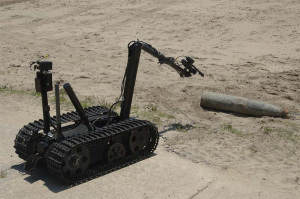
\includegraphics[scale=0.8]{FiguresSoA/militarRobot}\label{fig:robotMilitar}}
%\subfigure[Vehículo aéreo no tripulado]{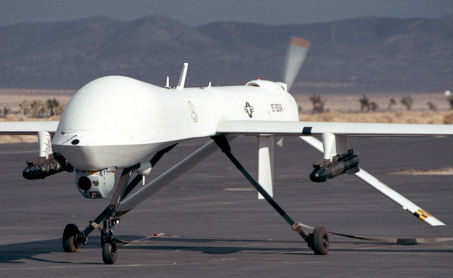
\includegraphics[scale=0.7]{FiguresSoA/drone}\label{fig:drone}}
%\caption{Ejemplos de Robot Teleoperados}
%\end{figure}



%Applications
%Telerobotics for Space
%Soviet telerobotic vehicle Lunokhod-1

%With the exception of the Apollo program most space exploration has been conducted with telerobotic space probes. Most space-based astronomy, for example, has been conducted with telerobotic telescopes. The Russian Lunokhod-1 mission, for example, put a remotely-driver rover on the moon, which was driven in real time (with a 2.5-second lightspeed time delay) by human operators on the ground. Robotic planetary exploration programs use spacecraft that are programmed by humans at ground stations, essentially achieving a long time-delay form of telerobotic operation. Recent noteworthy examples include the Mars exploration rovers (MER) and the Curiosity rover. In the case of the MER mission, the spacecraft and the rover operated on stored programs, with the rover drivers on the ground programming each day's operation. The International Space Station (ISS) uses a two-armed telemanipulator called Dextre. More recently, a humanoid robot Robonaut[2] has been added to the space station for telerobotic experiments.

%NASA has proposed use of highly capable telerobotic systems[3] for future planetary exploration using human exploration from orbit. In a concept for Mars Exploration proposed by Landis, a precursor mission to Mars could be done in which the human vehicle brings a crew to Mars, but remains in orbit rather than landing on the surface, while a highly capable remote robot is operated in real time on the surface.[4] Such a system would go beyond the simple long time delay robotics and move to a regime of virtual telepresence on the planet. One study of this concept, the Human Exploration using Real-time Robotic Operations (HERRO) concept, suggested that such a mission could be used to explore a wide variety of planetary destinations.[5]

%NASA HERRO (Human Exploration using Real-time Robotic Operations) telerobotic exploration concept[5]

%Telepresence/Videoconferencing

%The prevalence of high quality video conferencing using mobile devices, tablets and portable computers has enabled a drastic growth in Telepresence Robots to help give a better sense of remote physical presence for communication and collaboration in the office, home, school, etc. when one cannot be there in person. The robot avatar can move or look around at the command of the remote person.[6]

%There have been two primary approaches that both utilize videoconferencing on a display 1) desktop telepresence robots - typically mount a phone or tablet on a motorized desktop stand to enable the remote person to look around a remote environment by panning and tilting the display or 2) drivable telepresence robots - typically contain a display (integrated or separate phone or tablet) mounted on a roaming base Some examples of desktop telepresence robots include Kubi by Revolve Robotics, Galileo by Motrr, and Swivl. Some examples of roaming telepresence robots include Beam by Suitable Technologies, Double by Double Robotics, RP-Vita by iRobot, Anybots, Vgo, TeleMe by Mantarobot, and Romo by Romotive.

%For over 20 years, telepresence robots, also sometimes referred to as remote-presence devices have been a vision of the tech industry. Until recently, engineers did not have the processors, the miniature microphones, cameras and sensors, or the cheap, fast broadband necessary to support them. But in the last five years, a number of companies have been introducing functional devices. As the value of skilled labor rises, these companies are beginning to see a way to eliminate the barrier of geography between offices.[7] Traditional videoconferencing systems and telepresence rooms generally offer Pan / Tilt / Zoom cameras with far end control. The ability for the remote user to turn the device’s head and look around naturally during a meeting is often seen as the strongest feature of a telepresence robot. For this reason, the developers have emerged in the new category of desktop telepresence robots that concentrate on this strongest feature to create a much lower cost robot. The Desktop Telepresence Robots, also called Head and Neck Robots allow users to look around during a meeting and are small enough to be carried from location to location, eliminating the need for remote navigation.[8]



%\subsection{Aplicaciones Maritimas de la Telerobótica}
%
%%Marine Applications
%
%Los vehículos Marinos Operados Remotamente han sido ampliamente usados para trabajar en aguas profundas o demasiado peligrosas para los buzos.
%
%\begin{figure}
%\centering
%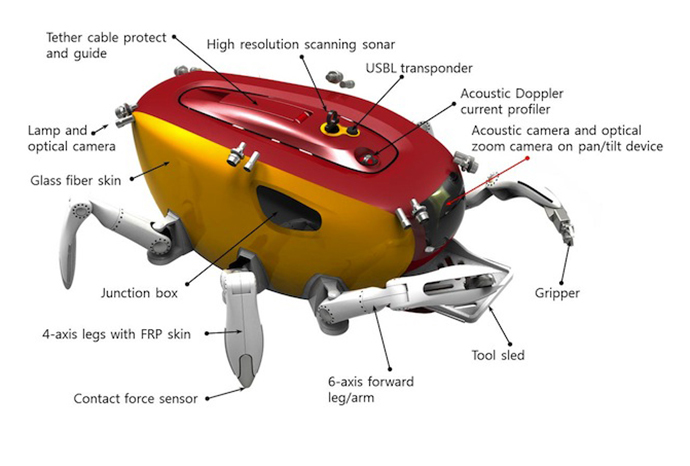
\includegraphics[scale=0.7]{FiguresSoA/crabster}
%\caption{Robot Crabster o CR200 desarrollado por el Instituto Coreano de Tecnología y Ciencias del Oceano }
%\label{fig:cr200}
%\end{figure}
%
%Investigadores del Instituto Coreano de Tecnología y ciencias del Oceano, desarrollaron el robot teleoperado Crabster o CR200 (ver figura \ref{fig:cr200}), diseñado para caminar en el fondo oceánico y soportar las corrientes marítimas, como un crustaceo.\\
%
%El CR200 promete tener todas las posibilidades de ser el robot submarino hexápodo  más grande y ágil del mundo
%
%Las dimensiones del CR200 son de 2.4 m de largo, 2.4 m de ancho y 1.8 metros de alto con sus patas extendidas
%% It’s also way bigger than real crabs: It’s 2.4 meters long, 2.4 meters wide and – when its legs are fully extended – 1.8 meters high.
%
%
%Sus creadores afirman que uno de los mayores retos fue que el CR200 pudiese alcanzar una velocidad de 10 cm/ segundo
%
%los creadores del cr200 esperan que su revolucionario diseño permita hacer construcciones en el fondo del mar. El cr200 puede alcanzar una profundidad de 200 m. y adaptar su postura a diferentes condiciones de presión.


%But it’s also a good deal slower than one of Mother Nature’s crabs, and its creators say that its speed of 10cm/second is one of their main challenges, since it’s difficult to improve Crabster’s stability in strong currents and on rough terrain.



%CR200 hopes to revolutionize the way underwater craft are developed in the future. It can operate down to a depth of 200 meters and adapt its posture to different pressure conditions.

%"We suppose CR200 can conduct seabed mapping, survey and inspection of wrecks, pipelines, ecosystems and pollution down to a 200-meter depth. CR200 will help divers or work instead of them in harsh environments. It also could assist in locating underwater resources, carrying out underwater mining, and responding to oil spill incidents," he said.

%La idea del diseño del cr200 es que pueda hacer un mapeo de las profundidades del mar



%Crabster, designed to scuttle across the ocean floor and survive strong ocean currents and tides just like a real crustacean, has all the chances to be the world’s largest and most agile underwater walking robot, its project team boasts.

%A new crab-like robot is being released into the oceans by the Korean Institute of Ocean Science and Technology.

%CR200, or Crabster as it is affectionately called by its creators, weighs in at over half a ton and has six walking legs, unlike its natural brothers, who have eight. 



%The peculiar design for the robot was chosen as crabs and lobsters can easily control their movements even though they live in stormy waters. Current propeller-driven submersibles do not work properly in fierce tides and human divers are limited to calm, shallow seas.


%It is also kitted out with sonar to scan the seabed for objects of interest, and can send images up to the surface through onboard cameras. 


% Bong Huan jun, the lead researcher of the project, said the robot had performed very well in initial tests but was still undergoing continuous modifications.

%“We are performing tests nearly every day. We upgrade Crabster software for more stable and fast walking and manipulation,” he told CNN.

%The robotic crab will perform its first mission in May, when it will be looking for ancient artifacts in the Yellow Sea where existing craft have been unsuccessful.

%Should this maiden voyage be a success, then Huan jun believes it will have a large worldwide impact.


%He said his team is trying to make Crabster more versatile by trying to program it to swim like a turtle or a diving beetle. They are also considering a hydraulic version for heavy duty underwater work.

%He said he wasn’t sure if the other inhabitants of the deep would know for sure if he is a real crab or not, but said that he hoped that “animals would treat him friendly.” 




%Marine remotely operated vehicles (ROVs) are widely used to work in water too deep or too dangerous for divers. They repair offshore oil platforms and attach cables to sunken ships to hoist them. They are usually attached by a tether to a control center on a surface ship. The wreck of the Titanic was explored by an ROV, as well as by a crew-operated vessel.


\subsection{Telerobótica Médica}


\begin{figure}[htp!]
\centering
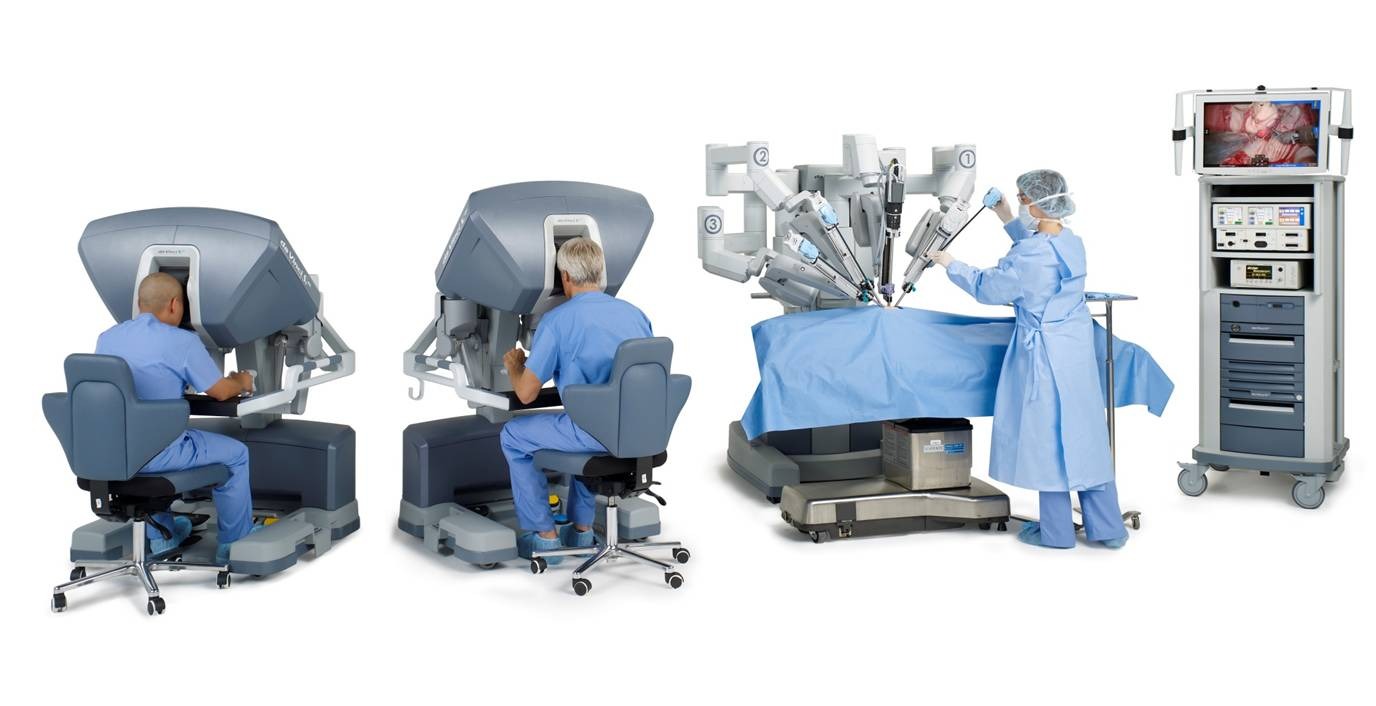
\includegraphics[scale=0.65]{FiguresSoA/News-Da-Vinci-Surgical-Robot-4}
\caption[dos cirujanos ]{Dos cirujanos trabajando de forma cooperativa con el Robot Quirurgico Da Vinci}
\label{fig:davinci1}
\end{figure}


Actualmente se han sido realizadas  grandes esfuerzos e investigaciones en el área de los dispositivos médicos, especialmente para cirugía de mínima invasión. Con los actuales sistemas de cirugía robóticos y de cirugía mínima invasiva los cirujanos son capaces de operar a un paciente a través de un pequeño orificio solo lo suficientemente grande como para permitir la inserción de instrumentos especialmente diseñados, eliminando la necesidad de abrir grandes cavidades que permitiesen trabajar con las manos como se realizaba antiguamente.\\


El Sistema da Vinci es un ejemplo de los últimos desarrollos en el área de la medicina a distancia. El sistema es utilizado para múltiples procedimientos quirúrgicos, especialmente en prostatectomías, es controlado por un cirujano que opera desde una consola y se diseñó para facilitar la cirugía compleja empleando un enfoque mínimamente invasivo. Este factor permite superar las limitaciones propias de la cirugía abierta y laparoscópica, potenciando en términos de visión, precisión y control las habilidades del cirujano. El robot da Vinci no es autónomo,y por ello requiere en todos los casos la intervención y toma de decisiones de un profesional que actúe como operador humano para todas las acciones.\\


El robot quirúrgico Da Vinci se compone de una consola ergonómica desde la que el cirujano opera sentado y que, normalmente, se encuentra en el mismo quirófano. Al lado del paciente se sitúa la torre de visión (formada por controladores, vídeo, audio y proceso de imagen) y el carro quirúrgico que incorpora tres o cuatro brazos robóticos interactivos controlados desde la consola, en el extremo de los cuales se encuentran acopladas las distintas herramientas que el médico necesita para operar, tales como bisturís, tijeras, unipolar, entre otras.\\


El robot da Vinci permite optimizar el rango de acción de la mano humana, reduciendo el posible temblor y perfeccionando todos los movimientos del cirujano. De esta manera, se minimizan las posibilidades de error en relación a otros sistemas quirúrgicos como la laparoscopia, procedimiento en el que el cirujano debe operar de pie con una visión del área anatómica en la que interviene en 2D. En contraposición, el da Vinci ofrece una visión tridimensional de la zona intervenida. Por otro lado, en la laparoscopia, el médico depende de un ayudante para posicionar la cámara correctamente, mientras que en el da Vinci, el cirujano gestiona la cámara de forma totalmente autónoma. También es importante subrayar que el instrumental de la laparoscopia ofrece unos índices de versatilidad limitados mientras que los instrumentos del da Vinci pueden operar de igual forma a cómo lo haría una muñeca humana, lo que permite realizar movimientos altamente precisos en espacios muy reducidos.\\


Otro valor añadido de gran relevancia que ofrece el robot da Vinci al profesional es la posibilidad de poder contar con una visión superior en 3D, alineada entre la zona anatómica afectada y el instrumental, una posición única desde la que se puede trabajar de forma cómoda, intuitiva y precisa.\\


Algunas características del sistema son:
\begin{description}


\item[Consola ergonómica del cirujano]
Es el centro de mando del sistema Da Vinci Si. El cirujano se sienta fuera del campo estéril, en la consola del cirujano, y maneja un endoscopio en 3D y los instrumentos EndoWrist® con los ojos, las manos y los pies mediante dos controladores principales y pedales. El sistema interpreta los movimientos del cirujano y los traduce a escala con movimientos precisos de los instrumentos.

\item[Carro Quirúrgico]
Es el componente quirúrgico del sistema Da Vinci Si, y su función principal es sostener los brazos para instrumentos y el brazo para la cámara. El sistema Da Vinci Si, utiliza la tecnología de centro de control. El centro de control es un punto fijo alrededor del cual se mueven los brazos del carro del paciente. La tecnología de centro de control, permite que el sistema manipule los instrumentos y el endoscopio en la zona de la operación, ejerciendo la mínima presión en la pared del cuerpo del paciente. El usuario del carro del paciente trabaja en el área estéril, ayudando al usuario de la consola del cirujano con el intercambio de instrumentos y endoscopios, y con otras tareas en la zona del paciente. Para garantizar la seguridad del paciente, las acciones del carro del paciente tienen prioridad sobre las acciones de la consola del cirujano.

\item[Torre de Visión]
Aloja el equipo de visualización de procesamiento central del sistema. Posee estantes regulables para incorporar instrumentos quirúrgicos auxiliares opcionales, como unidades electroquirúrgicas (ESU) e insufladores. Durante la operación lo maneja una persona no estéril.


\end{description}



En la figura \ref{fig:davinci1} puede apreciarse  el robot Da Vinci siendo manipulado por dos dispositivos maestros lo cual permite el trabajo colaborativo de ambos, incluso sin la necesidad de estar en el mismo sitio.\\

El robot permite alta precisión de los movimientos ejecutados por el cirujano y el uso de una gran cantidad de instrumentos quirúrgicos distintos de los que cada día se desarrollan más cada día se están desarrollando más instrumentos.\\

La implementación de este sistema permite que los cirujanos puedan trabajar prácticamente desde cualquier parte del mundo.\\


%el robot esclavo Da Vinci cuenta con 4 brazos de 6 grados de libertad cada uno (Ver figura \ref{fig:davinci2}), 

%
%\begin{figure}
%\centering
%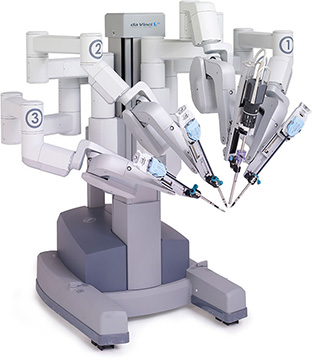
\includegraphics[scale=0.6]{FiguresSoA/davinci-robot}
%\caption{Robot Quirurgico Da Vinci (Esclavo)}
%\label{fig:davinci2}
%\end{figure}

\subsection{Manipuladores Remotos para Entornos Radioactivos}

Los entornos de fusión nuclear están fuertemente restringidos por varios factores, tales como la radiación, altas temperaturas y las dimensiones y pesos de sus componentes. Esto obliga a considerar el diseño de tecnologías de teleoperación como una estrategia viable para realizar tareas en dichas instalaciones.
La fusión nuclear como fuente de energía requerirá el desarrollo de varias tecnologías de teleoperación que pueden ser automáticas o manuales.

Las futuras plantas de energía de fusión similares a la planta de demostración (DEMO) requerirán un sistema de teleoperación excepcional para llevar a cabo actividades de supervisión y mantenimiento. Estas tareas desempeñan un papel fundamental en la gestión global de una planta de energía nuclear.

Las tecnologías de teleoperación se han utilizado con éxito en células de fisión nuclear durante mucho tiempo \cite{Desbats2005} y en el mantenimiento del \textit{tokamak} del \textit{Joint European Torus} (JET) por más de 10 años \cite{Rolfe1999, Rolfe2007} ya que con ello se evitan paradas inesperadas, retrasos de mantenimiento, etc. Además, se ha mejorado la seguridad del personal mediante la reducción de exposición a la radiación y el aumento de la disponibilidad del reactor mediante el uso de equipo reforzado para resistir las condiciones de operación tan cr\'iticas.

En esta sección se presentan los requisitos y características que deben cumplir los sistemas de telerrobótica en un entorno de fusión nuclear. En \cite{Ferre2011,Suarez2011,Queral2011} se presentan estudios completos sobre dichos requisitos y características.

\subsection*{Motivación}
En los últimos años, el establecimiento de la fusión nuclear como fuente de energía requerirá el uso de sistemas teleoperados debido principalmente a la radiación. La industria nuclear ha utilizado los sistemas remotos debido a las restricciones de su entorno desde el principio, pero con los avances tecnológicos se impulsa la implementaci\'on de sistemas cada vez m\'as innovadores.\\

  
Dichos sistemas teleoperados deben hacer frente a: altos niveles de radiación, ultra-vacío, altas temperaturas y el campo magnético toroidal con la intención de realizar la inspección, mantenimiento y reparación de instalaciones de fusión nuclear, tales como el Reactor Termonuclear Experimental Internacional (ITER), DEMO o \textit{International Fusion Materials Irradiation Facility} (IFMIF).

\subsection*{Radiación}
En la tabla~\ref{tab:radiation} se muestran las dosis de radiación para el caso de ITER \cite{ITEROrg.2004}.
\begin{table} [htbp]
\centering
	\caption{Dosis de Radiación para ITER}
	\label{tab:radiation}
	\begin{tabular}{c c c c}
		\hline
		 & \multicolumn{3}{c}{\textbf{Tipo de Inspección}} \\ 
		 																& \textbf{Programada} 	& \textbf{Sin Programar} 		& \textbf{Mantenimiento }\\ 
		\hline
		\multicolumn{1}{l}{\textbf{Tasa de Dosis (Gy/h)$^*$}} 		& $1500$ 							& $15000$ 								& $300$ \\ 
		\multicolumn{1}{l}{\textbf{Duración}} 								& 12 h/semana 					& 12 h/semana 							& 60 h/mes \\ 
		\multicolumn{1}{l}{\textbf{Periodo}}									& $7.5$ años 						& $7.5$ años 								& 32 meses \\ 
		\multicolumn{1}{l}{\textbf{Dosis Total (MGy)}} 	& $2.7$ 								& $27$ 										& $0.6$ \\ 
		\hline
		\multicolumn{4}{l}{$^*$ \small{Datos estimados}}\\
	\end{tabular} 	
\end{table}
El funcionamiento de la electrónica es un problema importante cuando se trata de entornos con radiación\cite{Perrot2004}.
A pesar que varios sistemas de multiplexación no soportan más de 10 kGy, algunos transistores manejan valores nominales de hasta 10MGy.Por lo tanto, es de esperar que sea posible diseñar componentes resistentes hasta 10MGy con estos transistores.El \textit{Radiation Hardness Manual} \cite{Campbell2007} cuenta con un listado de circuitos digitales (flip-flops y compuertas) basados en transistores discretos que resisten dosis en el rango de 10MGy. Por ejemplo, todos los componentes electrónicos del robot PAC \cite{Perrot2004}, descrito en el numeral \ref{robotPAC:sub}, soportan una dosis total de hasta 10 kGy, con una tasa máxima de 10Gy/h.

Todos los materiales estructurales no deben ser susceptibles a la degradación por contaminación.
Componentes sensibles como los sellos deben ser elegidos de acuerdo a su resistencia a la radiación.
Teniendo en cuenta que la única barrera contra la radiación es la masa y que los requisitos dimensionales de los robots no permiten el uso de tales barreras de manera eficaz, todos los componentes a ser utilizados deben probarse para comprobar su funcionamiento bajo altas dosis de radiación.

Se han realizado varios estudios a una amplia gama de componentes con el fin de utilizarlos en la cámara de vacío del reactor, desde fibras ópticas hasta lubricantes, actuadores y cámaras de vídeo \cite{VanUffelen2005, Leroux2006, Bock2008}.Estos estudios muestran que ser\'a posible tener diseños electrónicos compatibles con las limitaciones del entorno de fusión nuclear.

\subsection*{Ultra-Vacío}
Debido a las ultra bajas presiones ($10^{-5} $ Pa) \cite {ITEROrg.2004}, la cámara de vacío (VV - \textit{Vacuum Vessel})  \'esta se debe mantener limpia a toda costa. As\'i, el uso de materiales que liberan gases debe ser evitado. Por lo general, materiales susceptibles a la oxidación y los materiales orgánicos, liberan gases. Por lo que todos los componentes que entran en contacto directo con la cámara de vacío tienen que ser certificados. Una lista de componentes y materiales aptos para ser utilizados en ultra-vacío se puede encontrar en el \textit{ITER Vacuum Handbook} \cite{L.Worth2009}.
El material estructural predeterminado por ITER para estas condiciones es el acero inoxidable 316L (N)-IG \cite{Aiello2011}.

Con el fin de eliminar todas las impurezas y burbujas de gases se realiza el coquizado del robot (normalmente a $240^{o}C $). Generalmente estos puntos que pueden liberar gases se encuentran situados en las imperfecciones de la estructura. El coquizado permite eliminar cualquier rastro de hidrógeno y oxígeno que queda en los poros de los materiales.
Cuando el robot no se puede coquizar en un plazo razonable, lo habitual es confinar en un espacio cerrado las zonas con porosidades.


Existen soluciones de sellado, como la utilizada en el robot AIA \cite{Keller2009}, descrito en la secci\'on \ref{robotAIA:sub}, donde se utiliza Helicoflex\textsuperscript{\textregistered} y sellos de metal.

Por otro lado, se deben utilizar lubricantes no estándar, tales como el disulfuro de molibdeno (MoS$ _ {2} $), carbón tipo diamante (DLC), diseleniuro de tugsteno (WSe$ _ {2} $), sulfuro de tungsteno (WS$ _{2} $) y diseleniuro de molibdeno (MoSe$ _ {2} $) \cite{ogawa2008research}.
En \cite{winer1967molybdenum} se puede encontrar una revisión completa sobre el comportamiento del MoS$ _ {2} $.
Además, el MoS$ _ {2}$ ha sido probado en ultra-vacío y se ha encontrado que ofrece un coeficiente de fricción muy bajo \cite{cizaire2002mechanisms}.
Esta técnica se ha utilizado ampliamente para el diagnóstico de reactores \cite{ogawa2008research}.

\subsection*{Altas Temperaturas}
Para ITER, en la tabla~\ref{tab:temperature} se muestra un resumen de las posibles temperaturas de operación en distintos escenarios \cite{ITEROrg.2004}.

\begin{table} [htbp]
\centering
	\caption{Posibles temperaturas durante inspección para ITER}
	\label{tab:temperature}
	\begin{tabular}{c c}
		
		\textbf{Descripción} 	& \textbf{Temperatura 1\textsuperscript{er} Pared}\\ 
		
		\multicolumn{1}{l}{\textbf{Inspección Programada}} 	& 			$393 K$   \\ 
		\multicolumn{1}{l}{\textbf{Inspección Durante Coquizado}} 	& 		$513 K$   \\ 
		\multicolumn{1}{l}{\textbf{Inspección sin Programar}} 		& 	$393 K$   \\ 
		\multicolumn{1}{l}{\textbf{Mantenimiento}} 					& 	$323 K$   \\ 
		
	\end{tabular} 	
\end{table}

Teniendo en cuenta las altas temperaturas, todas las propiedades de los materiales  (resistencia a la tracción, módulo de elasticidad, etc.) deben ser consideradas a $393 K$ pero el material también debe ser coquizado ($513 K$). Por ejemplo, la mayoría de las aleaciones de aluminio están prohibidas para fines estructurales, ya que debido a sus propiedades mecánicas no son adecuadas para estas temperaturas. Las experiencias con el brazo articulado de Inspección (AIA) \cite{Keller2009} y el sistema de diagnóstico \cite{Smick2005}, dicen que la lubricación puede ser un problema grave también.

\subsubsection*{Distribución de la Temperatura}
Si las diferentes partes del robot están a diferentes temperaturas, puede producirse un problema debido a la dilatación térmica, lo que puede resultar en grietas o estrés adicional en los materiales.

Una solución para evitar este problema consiste en diseñar el robot para alcanzar uniformemente $393 K $. En este caso, las partes exteriores del robot deben actuar como cuerpos negros, con el fin de calentar la totalidad del robot a esa temperatura.

También se deben elegir los materiales con constantes de dilatación cercanas. Para los materiales con constante de dilatación diferente es necesario tener especial cuidado durante la fase de diseño del robot, ya que todas las piezas serán fabricadas a temperatura ambiente ($293 K $  aprox.). Esto también puede ser un problema si la fase de pruebas tiene que hacerse a temperatura ambiente.

\subsubsection*{Aislamiento Térmico}
A pesar de los esfuerzos que se pueden hacer para encontrar componentes compatibles con las altas temperaturas, siempre habrán algunos componentes que no las soporten. En estos casos, la solución es confinar estos componentes en una jaula hecha de material reflectante y puesto que los robots estarán en un ambiente de ultra-vacío, el modo de transferencia de calor principal será la radiación y dicha jaula reflectante tardaría una gran cantidad de tiempo para obtener la temperatura nominal.\\


Por lo tanto un buen diseño implica que dichos componentes puedan estar trabajando durante un largo período de tiempo.\\


Las articulaciones del robot deben ser diseñadas teniendo en cuenta el aislamiento térmico con el fin de minimizar la transferencia de calor por conducción. Esta solución es exactamente la opuesta a la estrategia de distribución de la temperatura. Dado el caso en que estas dos soluciones deban ser utilizadas en un mismo robot, es recomendable trabajar con un modelo muy preciso para cada uno de los casos.

Es evidente que la obtención de un modelo es una dificultad real, ya que la distribuci\'on de temperaturas puede llegar a ser tan compleja como el diseño del montaje. Otro posible solución es diseñar un sistema enfriador con un fluido o gas frío y utilizar un intercambiador de calor fuera de la cámara de vacío.

\subsection*{Campo Magnético}
Un campo magnético tan elevado (3,3 | 6.5MAm $^ {-1} $ / 41000 | 82000Oe densidad de flujo magnético es 4,1 | 8.2T en el vacío) \cite{Izard2009}, en un gran volumen es una situación muy rara, que sólo se encuentra en el mundo de fusión. Incluso la intención de operar bajo estas condiciones un equipo  remoto es única. De hecho, sólo recientemente gracias a los imanes superconductores  es posible generar campos magnéticos sostenidos tan altos \cite{Kiyoshi2006}.\\


Los imanes de cobre pueden producir campos muy elevados (el récord actual es de 100T), pero en un período de tiempo muy limitado \cite{Kiyoshi2006}, por lo que el robot esperaría a que el pulso acabase para realizar las tareas. Hasta ahora, no se habían combinado más restricciones a la del campo magnético, tales como la radiación, altas temperaturas y ultra-vacío en el caso de la fusión nuclear. Sin embargo, los robots que operan bajo la influencia de campos magnéticos elevados no son una novedad, ya que investigadores de la Universidad Johns Hopkins han presentado un sistema robótico completamente compatible con la resonancia magnética \cite{Muntener2006}.\\


En lo que respecta al uso de componentes, aquellos que funcionan utilizando un campo magnético (bobinas de inductancia, transformadores con núcleos de hierro, etc) se verán saturados y serán afectados por fuerzas muy altas, con lo cual, deben ser sustituidos por dispositivos tolerantes al campo magnético como bobinas de aire y transformadores de cerámica \cite{izard2010hardening} .\\


La diferencia principal de una aplicación de fusión nuclear con cualquier máquina superconductora, en general, es que la máquina no está funcionando en el momento del mantenimiento o la inspección, por lo tanto, la perturbación del campo local se puede tolerar, con lo cual los dispositivos electrónicos y los sistemas electromecánicos están permitidos. Los efectos del campo magnético son descritos por las ecuaciones de Maxwell. El desarrollo de las ecuaciones de Maxwell conduce a la fuerza de Lorentz $\mathbf{F}_ {L} $. Cuando no hay ningún campo eléctrico, está escrito como,

\begin{equation}
	\label{ecu:lorentz1}
	\mathbf{F}_{L}=q\cdot{}\mathbf{v}\times{}\mathbf{B}
\end{equation}
En una carga $q$ que se mueve a una velocidad $\mathbf{v}$, ó,
\begin{equation}
	\label{ecu:lorentz2}
	F_{L}=i\cdot{}l\cdot{}\mathbf{u}\times{}\mathbf{B}
\end{equation}

En un conductor con una longitud $l$ y corriente $i$ a lo largo del vector $\mathbf{u}$. $\mathbf{B}$ es la densidad de flujo magnético local en ambas ecuaciones. La ecuación de la fuerza de Lorentz puede ser desarrollada con el fin de demostrar que un campo magnético elevado y constante puede producir un par elevado pero ninguna fuerza: un alto gradiente es necesario para generar una fuerza elevada en un volumen reducido \cite{Izard2009}.

\subsection*{Desarrollos Actuales}
Hoy en día aún no existe ningún robot capaz de soportar las condiciones impuestas por los entornos de fusión nuclear.
Los únicos sistemas que cumplen dichas restricciones son los de diagnóstico, pero deben operar incluso durante la fase de plasma y en muchas ocasiones no se pueden recuperar. Además, el diseño de estos sistemas los hace muy robustos y lejos de poder ser considerados como un robot completo. El sistema de visión \textit{In-Vessel Viewing System} (IVVS) \cite{Neri2007,Neri2009} desarrollado por la ENEA es un ejemplo de los mencionados sistemas de diagnóstico y de lo que se puede hacer con las condiciones dadas.

Dado que estos sistemas de diagnóstico no proporcionan la destreza necesaria para el funcionamiento en la cámara de vacío, la segunda parte de esta sección se centrará en los dispositivos que cumplen algunas de las restricciones, pero con niveles de destreza altos.

\subsection*{Sistema de Diagnóstico}
En fusión nuclear, el entorno de diagnóstico es aún más difícil que el entorno de inspección y mantenimiento, ya que además del ultra-vacío, el sistema de diagnóstico tiene que lidiar con enormes dosis de radiación y altas temperaturas. Además, se utilizan durante la operación del plasma y tienen que hacer frente a las corrientes parásitas (\textit{Eddy currents}) generadas a lo largo de su estructura en caso de un enfriamiento rápido \cite{Izard2009}.

Por estas razones, los sistemas de diagnóstico son muy robustos, sencillos y con capacidades de movimiento mínimas con el fin de evitar fallas. La regla general es el uso de actuadores neumáticos que generen un movimiento lineal. Otros sistemas como mecanismos accionados por temperatura y diseños que utilizan el campo magnético local para generar movimiento también se han utilizado en \textit{tokamaks} anteriores \cite{Smick2005} y esta prevista su utilización en ITER. En este entorno, parece que un gran porcentaje de la carga sobre los actuadores es debido a las corrientes parásitas generadas en las partes móviles \cite{Izard2009}.

%\subsection*{Sonda IVVS}
%El objetivo de la sonda IVVS (\textit{In-Vessel Viewing System}), figura~\ref{fig:IVVS}, para ITER es la medición y visión en la cámara de vacío en condiciones de inspección. En el prototipo construido por la Asociación Italiana de Fusión ENEA \cite{Perrot2004, Neri2007,Neri2009}, un láser se dirige hacia la cabeza de la sonda usando fibra óptica endurecida y luego hacia la pared en inspección utilizando un prisma cuya posición es ajustada por un accionamiento de dos grados libertad.
%
%\begin{figure}[htbp]
%   \centering
%   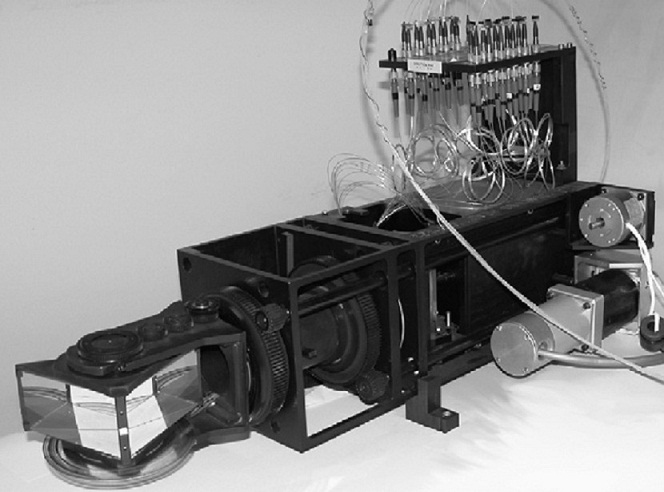
\includegraphics[width=0.5\textwidth]{FiguresSoA/IVVS}
%   \caption{Sonda IVVS}
%   \label{fig:IVVS} 
%\end{figure}
%
%En su último diseño, la sonda es de acero inoxidable AISI 304, pesa 22 Kg., tiene motores ultrasónicos y reductoras para mover el prisma. El marco del espejo es en aleación de titanio para reducir la fricción por las corrientes parásitas, ya que se supone que se mueva a 1 rps \cite{Izard2009}; Las reductoras también son de acero inoxidable AISI 304, con nitruro de titanio para su lubricación.

\subsection*{Brazo Articulado de Inspección AIA}		\label{robotAIA:sub}
El brazo articulado de Inspección AIA \cite{Gargiulo2008,Keller2009,Gargiulo2009, Houry2010}, que se muestra en la figura \ref{fig:AIA}, desarrollado en conjunto por CEA List y los laboratorios IRFM, es una demostración de cómo un brazo articulado de largo alcance puede ser un solución factible para la inspección en la cámara de vacío. Este robot ha sido diseñado para funcionar en ultra-vacío ($10^{-5}$ Pa) y a una temperatura de $120^{\circ}C$ (previamente coquizado a $200^{\circ}C$). Es un brazo de cinco módulos con una capacidad de carga de 10 Kg, con una longitud total de $7,4$ m y 160 mm de diámetro. Su peso total es de 130 Kg.

\begin{figure}[htbp]
   \centering
   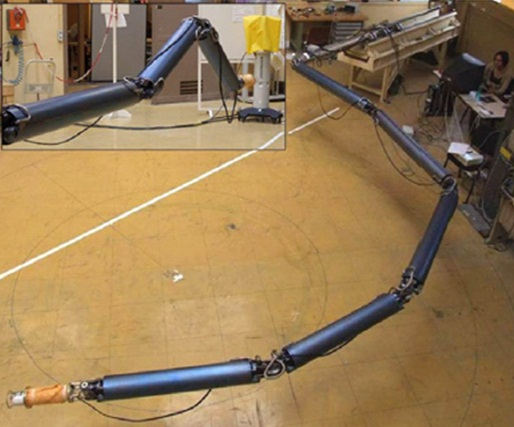
\includegraphics[width=0.6\textwidth]{FiguresSoA/AIA}
   \caption{Brazo Articulado de Inspección AIA}
   \label{fig:AIA} 
\end{figure}

La primera introducción del AIA en el reactor \textit{Tore Supra} en condiciones de operación tanto de ultra-vacío y temperatura se produjo en septiembre de 2008 \cite{Keller2009}.
Se equipó con una sonda de visión endurecida que le permitía observar la erosión de los casquetes limitadores y el funcionamiento de las persianas de diagnóstico.
Además cuenta con una amplia gama de efectores finales desde un láser para la eliminación de tritio hasta tareas ligeras de contacto y calibración de diagnóstico con herramientas de sujeción.
La operación del plasma se reanudó 15 horas después de retirar el robot que es el tiempo necesario para alimentar las bobinas superconductoras \cite{Gargiulo2009}.

La información se transfiere a los módulos gracias a los sistemas de multiplexación.
Cada módulo está equipado con una electrónica de multiplexación \textit{Neurobot} endurecida para las altas temperaturas. También está equipado con un sistema de amplificación para los motores.
Los componentes que no son compatibles con el ultra-vacío están encerrados en cajas anti-fugas de acero inoxidable.

\subsection*{Robot PAC}
\label{robotPAC:sub}
El robot PAC (\textit{The Porteur Articulé en Cellule}) \cite{Perrot2004} mostrado en la figura~\ref{fig:PAC}, es un brazo articulado de 6 metros de largo con una capacidad de carga de 1 Kg y un diámetro exterior de 100 mm.
Se ha desarrollado para aplicaciones de AREVA-NC por CEA LIST y ha sido diseñado para realizar tareas de inspección en celdas calientes. Dichas celdas se encuentran bajo condiciones atmosféricas y de temperatura normales, pero los niveles de radiación son altos, por lo tanto, el robot tiene que resistir una dosis total de 10 kGy.

\begin{figure}[htbp] 
   \centering
   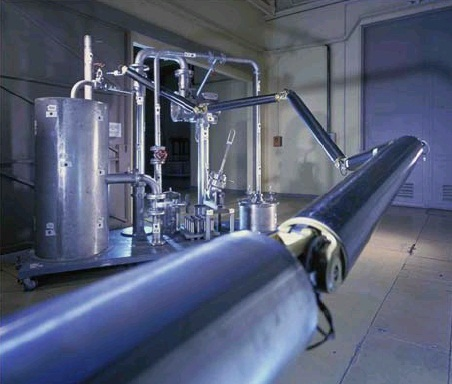
\includegraphics[width=0.6\textwidth]{FiguresSoA/PAC}
   \caption{Robot PAC en una celda caliente de AREVA.}
   \label{fig:PAC} 
\end{figure}

La principal característica demandada a este robot es la movilidad, ya que la celda caliente tiene tuberías complejas.
Es por eso que el robot tiene la misma arquitectura modular con el mecanismo paralelogramo vertical como el AIA en el cual se inspira. La diferencia es que en este caso el mecanismo de paralelogramo compensa la gravedad con un resorte de fibra de vidrio.

\subsection*{Manipulador WHMAN}
El manipulador WHMAN (\textit{Water Hydraulic MANipulator}) \cite{Nieminen2009} es un robot teleoperado con reflexión de fuerzas. Se caracteriza porque es hidráulico y como fluido utiliza agua. El brazo esta equipado con siete articulaciones actuadas que le permiten contar con seis grados de libertad. El diseño actual pesa 185 kg y sus materiales base son aleaciones de aluminio y acero inoxidable. Funciona con una presión de linea de 210 bar y requiere un caudal de 10 lpm. Además requiere una linea neumática a 6 bar y una conexión eléctrica.

\begin{figure}[htbp] 
   \centering
   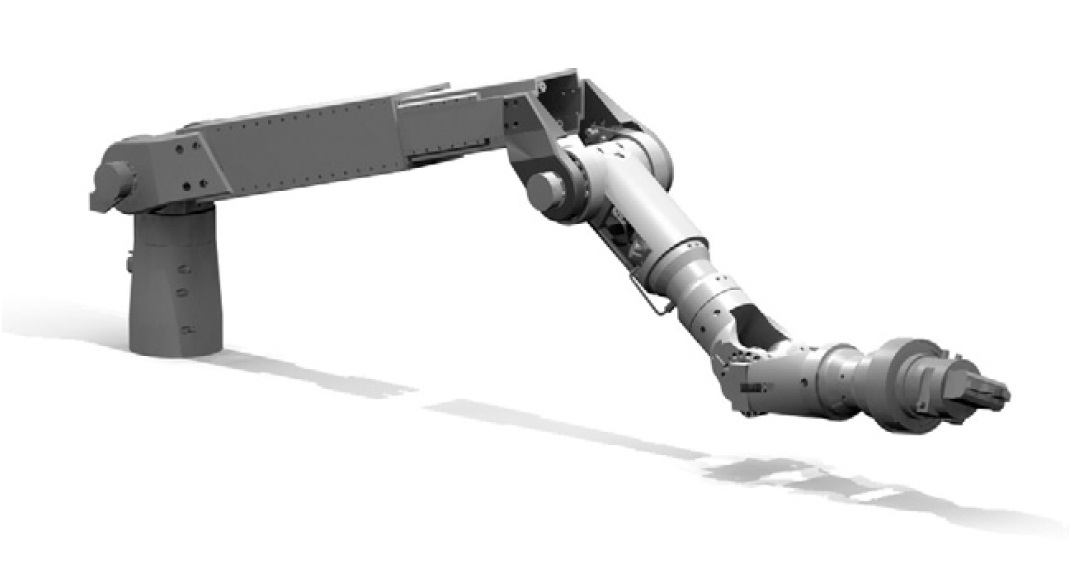
\includegraphics[width=0.7\textwidth]{FiguresSoA/WHMAN}
   \caption{Robot WHMAN de 6GDL.}
   \label{fig:WHMAN} 
\end{figure}

Tiene una capacidad de carga de 100 kg cuando esta totalmente extendido, en cuyo caso alcanza una distancia de 2.5 m medidos desde la articulación de la base. En la figura~\ref{fig:WHMAN} se muestra el diseño actual \cite{Nieminen2009}.
El WHMAN ha sido diseñado desde sus primeras fases para utilizar la potencia hidráulica del agua de acuerdo a los requisitos de ITER. Este manipulador es resistente a la radiación. Se estima que soporta una dosis de radiación de 300 Gy/h con una dosis acumulada de 1MGy. Debido a la elevada radiación, no utiliza electrónica digital, con lo cual, todos sus transductores est\'an basados en tecnología analógica.

%\subsection*{Robots MRI}
%Cabe mencionar que el reducida cantidad de máquinas superconductoras dará lugar a graves problemas logísticos cuando se quiera probar un robot completo bajo tales limitaciones.
%
%En pocas áreas, los robots se utilizan para posicionar objetos con precisión bajo la influencia de un alto campo magnético. Demuestra ser de interés para algunas intervenciones quirúrgicas. Es ahí donde aparecen los robots MRI. Un robot MRI es un robot médico capaz de operar dentro de una imagen de resonancia magnética (MRI), con el fin de realizar o ayudar en las intervenciones guiadas por imágenes (GII) \cite{Chinzei2001}.
%
%Hay pocos diseños para robots MRI, la mayoría de ellos trabajan lejos del campo magnético a fin de no sólo evitar la perturbación del dispositivo, sino también evitar la distorsión de la imagen como tal.
%En estos robots, tal como se presenta en \cite{Chinzei2001}, sólo las varillas largas pasivas de aleación de titanio o de material compuesto van en el campo magnético (\textless 0.5T).
%
%\begin{figure}[htbp]
%   \centering
%   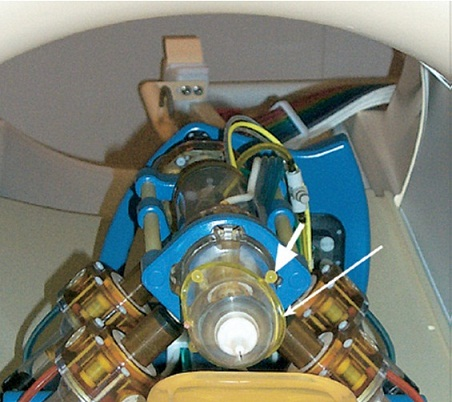
\includegraphics[width=0.5\textwidth]{FiguresSoA/MRI}
%   \caption{Robot MRI de al Universidad John Hopkins}
%   \label{fig:MIR} 
%\end{figure}
%
%Sin embargo, un equipo de la universidad John Hopkins ha sido diseñado un robot para funcionar con equipos de resonancias magnéticas \cite {Muntener2006}.
%Se dice que es el primer robot totalmente compatible con MRI y que cuenta con pruebas de compatibilidad de hasta 7T \cite{Muntener2006}.
%Dicho robot ha sido fabricado completamente con materiales paramagnéticos que evitan la distorsión del campo.
%Se basa en motores especiales, neumáticos, paso a paso y encoders ópticos con el fin de realizar movimientos precisos. Esto le permite manejar valores de precisión del orden de la fracción de milímetro. Es importante tener en cuenta que lo único que se le exige es ser compatible con resonancias magnéticas.



%\section{Telerobotica}
%Telepresence refers to a set of technologies which allow a person to feel as if they were present, to give the appearance of being present, or to have an effect, via telerobotics, at a place other than their true location.

%Telepresence requires that the users' senses be provided with such stimuli as to give the feeling of being in that other location. Additionally, users may be given the ability to affect the remote location. In this case, the user's position, movements, actions, voice, etc. may be sensed, transmitted and duplicated in the remote location to bring about this effect. Therefore information may be traveling in both directions between the user and the remote location.

%A popular application is found in telepresence videoconferencing, the highest possible level of videotelephony. Telepresence via video deploys greater technical sophistication and improved fidelity of both sight and sound than in traditional videoconferencing. Technical advancements in mobile collaboration have also extended the capabilities of videoconferencing beyond the boardroom for use with hand-held mobile devices, enabling collaboration independent of location.

%In a pioneering paper, Marvin Minsky attributed the development of the idea of telepresence to science fiction author Robert A. Heinlein: "My first vision of a remote-controlled economy came from Robert A. Heinlein's prophetic 1948 [sic] novel, Waldo," wrote Minsky. In his science fiction short story "Waldo" (1942), Heinlein first proposed a primitive telepresence master-slave manipulator system.

%The Brother Assassin, written by Fred Saberhagen in 1969, introduced the complete concept for a telepresence master-slave humanoid system. In the novel, the concept is described as follows: "And a moment later it seemed to all his senses that he had been transported from the master down into the body of the slave-unit standing beneath it on the floor. As the control of its movements passed over to him, the slave started gradually to lean to one side, and he moved its foot to maintain balance as naturally as he moved his own. Tilting back his head, he could look up through the slave's eyes to see the master-unit, with himself inside, maintaining the same attitude on its complex suspension."

%The term telepresence was coined in a 1980 article by the U.S. cognitive scientist Marvin Minsky, who outlined his vision for an adapted version of the older concept of teleoperation that focused on giving a remote participant a feeling of actually being present at a different location.[1]

%The first commercially successful telepresence company, Teleport (which was later renamed TeleSuite), was founded in 1993 by David Allen and Herold Williams.[2] Before TeleSuite, they ran a resort business from which the original concept emerged, because they often found businesspeople would have to cut their stays short to participate in important meetings. Their idea was to develop a technology that would allow businesspeople to attend their meetings without leaving the resorts so that they could lengthen their hotel stays.
%A Tandberg E20 high resolution videoconferencing phone meant to replace conventional desktop phones

%Hilton Hotels had originally licensed to install them in their hotels throughout the United States and other countries, but use was low. The idea lost momentum, with Hilton eventually backing out. TeleSuite later began to focus less on the hospitality industry and more on business-oriented telepresence systems. Shareholders eventually held enough stock to replace the company's original leadership, which ultimately led to its collapse.[citation needed] David Allen purchased all of the assets of TeleSuite and appointed Scott Allen as president, and Brian Kinne as EVP of the new company called Destiny Conferencing.

%Destiny Conferencing licensed its patent portfolio to HP which became the first large company to join the telepresence industry, soon followed by others such as Cisco and Polycom.[3] After forming a distribution agreement with Pleasanton-based Polycom, Destiny Conferencing sold on January 5, 2007 to Polycom for \$60 million.

%An important research project in telepresence began in 1990. Located at the University of Toronto, the Ontario Telepresence Project (OTP) was an interdisciplinary effort involving social sciences and engineering. Its final report stated that it "...was a three year, \$4.8 million pre-competitive research project whose mandate was to design and field trial advanced media space systems in a variety of workplaces in order to gain insights into key sociological and engineering issues. The OTP, which ended in December 1994, was part of the International Telepresence Project which linked Ontario researchers to their counterparts in four European nations. The Project’s major sponsor was the Province of Ontario, through two of its Centres of Excellence—the Information Technology Research Centre (ITRC) and the Telecommunications Research Institute of Ontario (TRIO)." [4]







\chapter{Plataforma Abierta de Teleoperación}
\begin{flushright}
\begin{minipage}{0,7\textwidth}
En este cap\'itulo se presenta el diseño de una arquitectura de control en tiempo real para una plataforma abierta de teleoperación compuesta por un brazo robótico de tipo antropomórfico. Este robot es actúa a través de dispositivos hidráulicos, operando en un entorno remoto y realimentando a un dispositivo maestro cinemáticamente idéntico, cerrando los bucles de control en fuerza. Son analizados los requerimientos de control para dispositivos hápticos. Se propone una arquitectura hardware/software. La arquitectura software propuesta se basa en técnicas de computación distribuida, la información acerca de ambos manipuladores se comparte por medio de una red local de internet.
\end{minipage}
\end{flushright}




\newpage
\section{Arquitectura General}

Como se muestra en la figura \ref{fig:arquitectura} el sistema robótico de teleoperación que se utilizar\'a en este trabajo se compone de las siguientes partes:\\

\begin{itemize}
\item Un manipulador hidráulico de seis grados de libertad (GDL) de la firma Kraft Telerobotics\textregistered
\item Un Efector final de tipo pinza
\item Dos controladores de tiempo real NI PXIe-1078
\item Un dispositivo maestro de seis grados de libertad
\end{itemize}

La arquitectura de control ha sido diseñada para compartir toda la información entre los sistemas maestro y el esclavo a través de Internet. En esta plataforma de teleoperación la información entre el maestro y el esclavo es compartida a través de una red local(LAN).\\


\begin{figure}[hbt!]
\caption{Arquitectura de la Plataforma de Teleoperacion}
\label{fig:arquitectura}
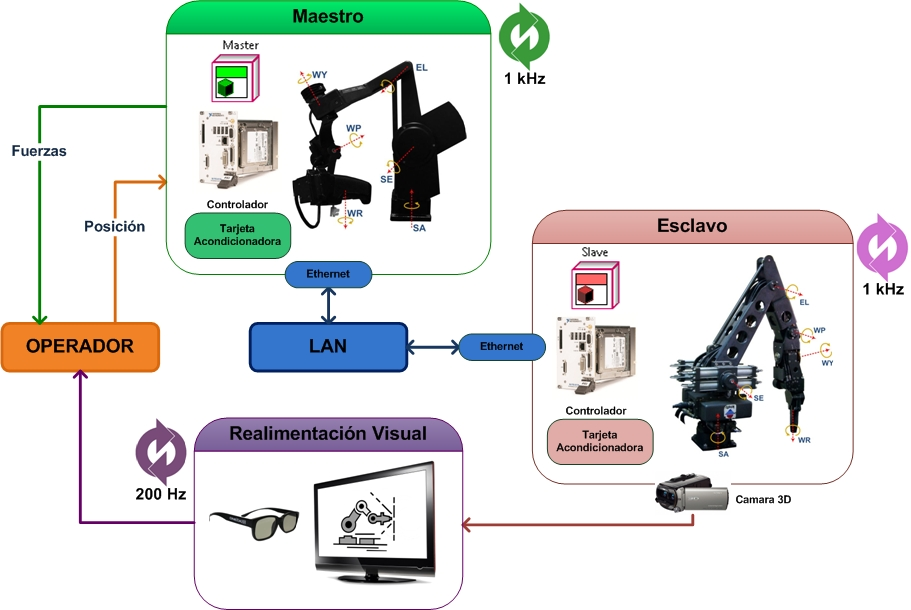
\includegraphics[scale=0.7]{FiguresP/ManufacturerArquitecture}
\end{figure}




El controlador de tiempo real del sistema maestro recibe mediciones de la posición y de la presión en los actuadores hidráulicos y la envía al controlador de tiempo real del dispositivo maestro que la procesa. El dispositivo maestro brinda una reflexión  de fuerzas al usuario basado en la información del esclavo, lee la posición actual de las articulaciones y calcula la posición y orientación del manipulador esclavo deseadas. El  dispositivo esclavo  usa esta información para  cerrar los bucles control (PI) de posición en cada articulación.\\

El protocolo de red utilizado para este sistema de teleoperación fue UDP (User Datagram Protocol). El protocolo UDP usa  un modelo de transmisión simple con un mecanismo mínimo\cite{zhao2006contrast} .

%Una de las ventajas del protocolo UDP
%La frecuencia ideal para los sistemas de teleoperación con reales de 1 KHz 


\section{Requerimientos del Sistema de Control}

En esta sección se describen las especificaciones de los componentes de la arquitectura de control para un sistema de teleoperación tipo maestro-esclavo 6 GDL. El sistema desarrollado debe contar con realimentación háptica  en los primeros tres  GDL, así como una realimentación visual y auditiva. La realimentación brindada al usuario es resultado de la interacción física con el entorno remoto.\\

Para lograr una transición suave en las gráficas o una realimentación visual aceptable es necesaria al menos una frecuencia de actualización de imágenes de al menos 50 Hz. en caso de requerirse una visión estereoscópica la frecuencia deberá aumentar por lo menos a 100 Hz. Uno de los requisitos de un sistema de teleoperaci\'on h\'aptico es que la frecuencia de realimentaci\'on visual sea suficiente para que el usuario tenga una experiencia similar a la que tendr\'ia si lo estuviera manipulando directamente. Es decir el usuario experimenta de forma coherente la información de forma visual y táctil. As\'i mismo la realimentación de fuerza también  requiere de una alta velocidad de actualización no solo para proporcionar una sensación realista sino también para asegurar la estabilidad. Se considera que es necesaria una frecuencia de actualización en tiempo real de al menos 1 KHz para alcanzar una sensación h\'aptica aceptable. Por otra parte los retardos en la transmisión de fuerzas pueden producir inestabilidades en el sistema h\'aptico al no ser consideradas en la fase de diseño.\\


 para sistemas de teleoperación sin realimentación háptica, las velocidades de actualización en tiempo real no son necesarias, debido a que la información visual es realimentada al usuario de forma unidireccional, dado que no afecta el comportamiento de los controladores del robot. 


El realismo de la interacción es denominado \textsc{transparencia}. La transparencia del sistema teleoperado es determinada por el algoritmo de control bilateral. Un requisito fundamental de un sistema de telemanipulaci\'on funcional es garantizar la estabilidad del sistema para todas las circunstancias que puedan ser encontradas durante la operación.\\


Para satisfacer estos requerimientos, se propone una arquitectura de red que procese las señales y realice los cálculos necesarios para el control del sistema en tiempo real. Esta arquitectura de control permite la conexión simult\'anea de los sistemas a través de Internet, lo cual es ideal para permitir una arquitectura abierta que permita a los desarrolladores programar y probar  sus aplicaciones  o estrategias de control.


%The realism of this reflected interaction is called the transparency of the system [1]. The obtainable transparency is amongst others
%determined by the implemented bilateral control algorithm. A fundamental requirement for a useful telemanipulation system is that it is guaranteed to be stable given all possible circumstances that can be encountered during operation.


\newpage
\section{Descripción detallada de la plataforma de teleoperaci\'on}

A continuación se describen algunos aspectos fundamentales a cerca de la plataforma experimental de teleoperación en la cual está basado el presente trabajo \cite{Galiana2012}. La intenci\'on es mejorar algunos aspectos físicos de la misma con la finalidad de conseguir un mejor rendimiento en cuanto a percepción del operador y con ello conseguir un menor tiempo en la ejecución de distintas tareas aplicando distintos algoritmos de control bilateral.\\

Se ha partido de dispositivos existentes en el grupo de investigación, dado que la realización de una plataforma de teleoperación supone un elevado coste y una gran inversión de tiempo. Se propone que sea totalmente abierta, con el propósito de que no solamente permita comprobar experimentalmente los algoritmos presentados, sino que adem\'as permita realizar cualquier otro tipo de pruebas, experimentos o investigaciones en el área de teleoperación.\\

Los movimientos ejercidos en el brazo maestro son reproducidos en el robot esclavo. Se caracteriza porque utiliza la arquitectura de control Fuerza - Posición, con lo cual el sistema mediante el maestro refleja fuerzas (alrededor del 10\%) al operador para que pueda tener una mejor percepción de la interacción del esclavo con el entorno. La reflexión de fuerzas es posible gracias a que el maestro cuenta con motores eléctricos en sus primeras cinco (5) articulaciones. Gracias a la reflexión de fuerzas el operador es capaz de realizar operaciones más complejas \cite{Ming1989,Hannaford1991}.\\


Se parte  del telemanipulador comercial GRIPS de Kraft Telerobotics Inc. del tipo maestro-esclavo, cuyas características se muestran en la tabla \ref{tab:espgrips}. Est\'a diseñado para operar en condiciones hostiles, bajo el agua e incluso en ambientes con radiación electromagnética y  nuclear bajo ciertas condiciones gracias a que elsistema esclavo es accionado hidráulicamente por válvulas reguladoras de caudal que al ser actuadas por medio de solenoides no son afectadas por dichas condiciones. En la tabla  \ref{tab:Plat:valves} se muestran las especificaciones de las mismas.


\begin{table}
  \centering
\caption{Espeficicaciones del robot esclavo GRIPS}
\label{tab:espgrips}
\begin{tabular}{c c}
\hline
Alcance horizontal & 1289 mm\\
Alcance vertical & 1566 mm\\
Altura de almacenamiento & 877 mm\\
Capacidad de carga & 82 kg\\
Capacidad de carga totalmente extendido & 45 kg\\
Grados de libertad & 6 + pinza\\
Torque de rotación en la muñeca & 20 Nm \\
Efector final & Gripper paralelo\\
Apertura & 100mm\\
Fuerza de agarre & 0-890 N\\
\textbf{Rango de las articulaciones} \\
SA-Shoulder Azimut & $180 \deg$\\
SE-Shoulder Elevation & $120 \deg$\\
EL-Elbow Pivot & $110 \deg$\\
WP-Wrist Pitch & $100 \deg$\\
WY-Wrist Yaw & $105 \deg$\\
WR-Wrist Rotation: \\
modo 1 & $180 \deg$\\
modo 2 & 0-40 rpm\\
\textbf{Peso}\\
En aire & 59 kg\\
En agua de mar & 41 kg\\
\textbf{Requisitos hidráulicos}\\
Presión nominal & 104-207 bar\\
Caudal nominal & 11 lpm\\
filtración absoluta & 25 micrones\\
Linea de presión & No.  6 JIC\\
Linea de retorno & No.  8 JIC\\
\hline
\end{tabular}
\end{table}




\begin{table}[htbp]
  \centering
  \caption{Características de las servoválvulas del manipulador esclavo}
    \begin{tabular}{ccc}
    \hline
    \textbf{Descripción} & \textbf{Valor} & \textbf{Unidades}\\
    \hline
    Caudal Nominal		& $1.5$		& gpm \\
    $\Delta P$			& $1000$	& psi \\
    Presión Nominal		& $1500$	& psi \\
    Impedancia Bobina	& $125$		& $ \Omega $ \\
    Corriente Bobina	& $20$		& mA \\
    \hline
    \end{tabular}%
  \label{tab:Plat:valves}%
\end{table}%


%En la figura \ref{fig:maestroesclavo} puede apreciarse el esquema de control de la plataforma el cual tiene una frecuencia de refresco de 1 Khz, para mantener la estabilidad del sistema control.


%\begin{figure}
%\centering
%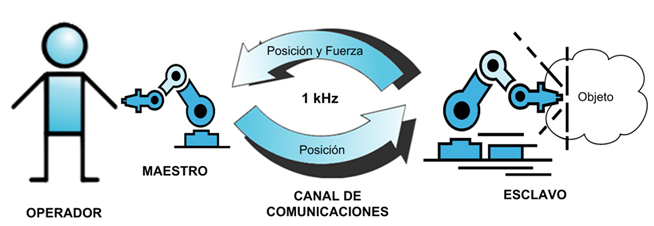
\includegraphics[scale=0.4]{FiguresP/MaestroEsclavo}
%\caption{Esquema de Control Maestro Esclavo}
%\label{fig:maestroesclavo}
%\end{figure}

%En la figura \ref{fig:maestro} se aprecia el dispositivo maestro del sistema de teleoperación, se muestran los ejes de movimiento.







\section{Sistema Esclavo}

Como sistema esclavo se tiene un brazo rob\'otico de seis grados de libertad con una pinza como efector final (ver figura \ref{Esclavo}), operado a base de actuadores hidr\'aulicos, sensores de presi\'on y posición.


\subsection{Sensores y Actuadores}

\begin{figure}
\centering
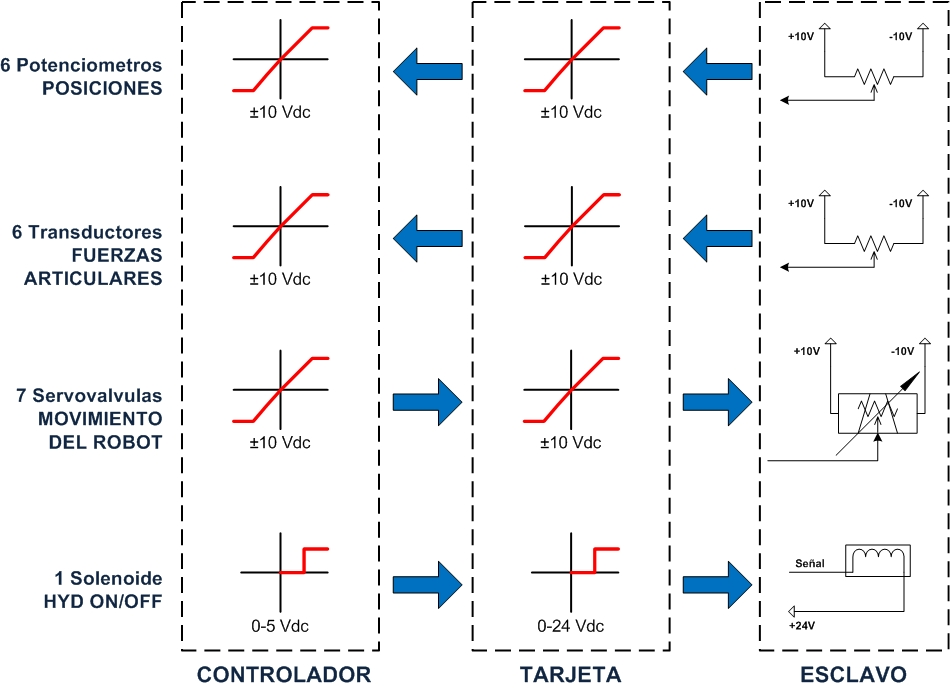
\includegraphics[scale=1]{FiguresP/EsquemaTarjetaEsclavo}
\caption{Esquema de la tarjeta de acondicionamiento de señales del dispositivo maestro}
\label{fig:EsquemaTarjetaEsclavo}
\end{figure}

\subsection*{Sensores}
La posición del robot se puede determinar gracias a los seis potenciómetros acoplados a cada grado de libertad. La fuerza ejercida por cada articulación y la pinza, con excepción de \textsc{Wrist Rotate} WR, es estimada por seis transductores de presión localizados en el colector de las válvulas. Las medidas obtenidas con estos transductores tienen suficiente precisión como para cerrar lazos de control \cite{Ferre2007a}. Las mediciones se realizan a través de un modulo de adquisición de datos conectado al bus del controlador de tiempo real, pasando primero por una etapa de acondicionamiento de señal (ver figura \ref{fig:TarjetaEsclavo})




\begin{figure}[htb]
\centering
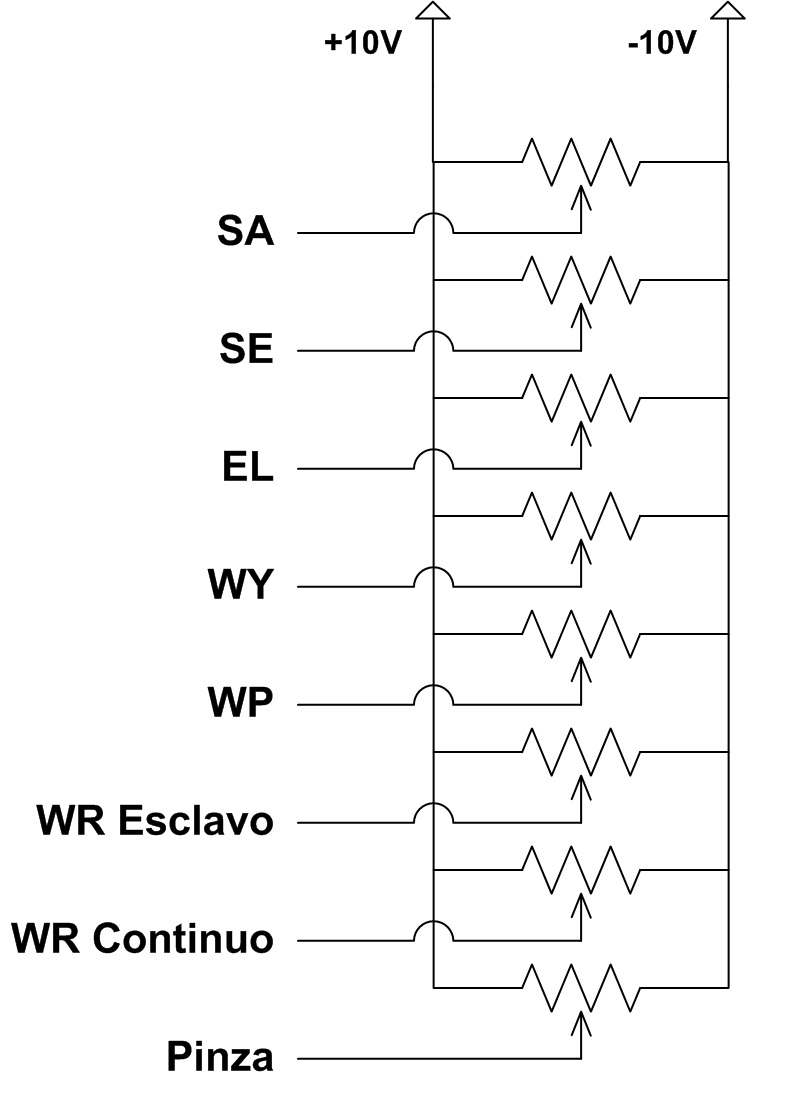
\includegraphics[scale=0.4]{FiguresP/Potenciometros}
\caption{Potenci\'ometros para medir la posición angular de cada una de las articulaciones}
\label{fig:potenciometros}
\end{figure}


\begin{figure}[htb!]
\centering
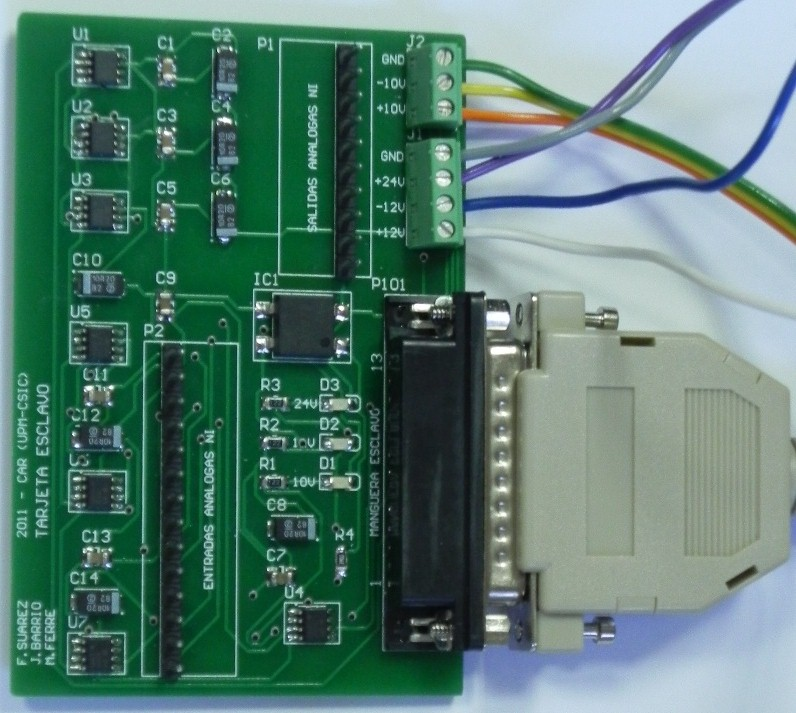
\includegraphics[scale=0.9]{FiguresP/TarjetaEsclavo}
\caption{Tarjeta del de acondicionamiento de señal del dispositivo Esclavo}
\label{fig:TarjetaEsclavo}
\end{figure}



\subsection*{Actuadores}
Cuenta con un conjunto de cilindros hidráulicos gobernados por  siete servoválvulas reguladoras de caudal que permiten regular el movimiento, además de una electroválvula que suministra la presión hidráulica al manipulador. La distribución de los actuadores permiten tres movimientos de brazo, tres movimientos de muñeca y la función de agarre de la pinza. Todos los movimientos, con excepción de WR y el cierre de la pinza, son trasmitidos utilizando actuadores tipo piñón - cremallera. El actuador de WR esta compuesto por un pistón tipo motor junto a una reductora con lo cual es posible realizar la rotación continua. Un pistón es utilizado para abrir y cerrar la pinza. 






\subsection{Cinemática Directa}

Es un manipulador del tipo antropomórfico de seis grados de libertad con una muñeca esférica con los siguientes parámetros de Denavit-Hartenberg

\begin{figure}[htb!]
\centering
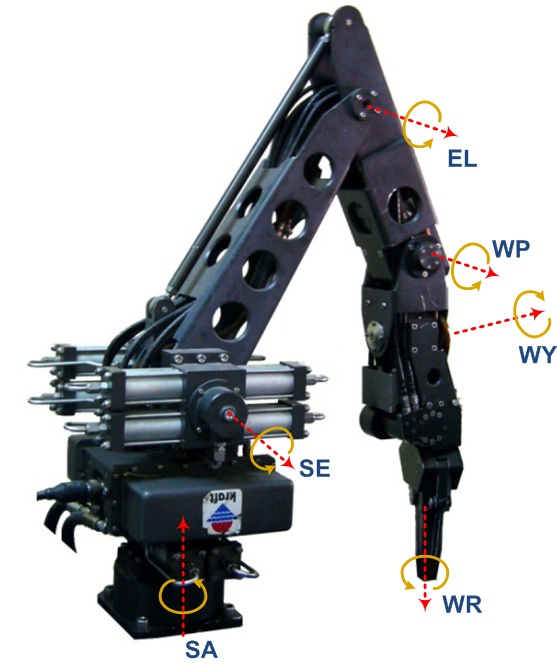
\includegraphics[scale=0.45]{FiguresP/EsclavoKraft}
\caption{Robot Esclavo }
\label{Esclavo}
\end{figure}



\begin{table}[htb!]
\caption{Parámetros de Denavit-Hartenberg para el robot esclavo GRIPS}
\centering
\label{tab:dhslave}
\begin{tabular}{ c c c c c }
 \hline
 Articulación & $a_i$ & $\alpha_i$ & $d_i$ & $\theta_i$ \\
 \hline
 1-SA 			& 0      & $-\frac{\pi}{2}$  & $l_1$     & $q_1$\\
 2-SE 			& $l_2$	 & 0                 & 0     & $q_2$\\
 3-EL 			& $l_3$	 & 0				    & 0     & $q_3$\\
 4-WP 			& $l_4$  & $\frac{\pi}{2}$   & 0     & $q_4$\\
 5-WY 			& 0      & $\frac{\pi}{2}$   & 0     & $q_5+\frac{\pi}{2}$\\
 6-WR 			& 0		 & 0                 & $l_6$     & $q_6$\\
 \hline
\end{tabular}
\end{table}



A partir de los parámetros de la tabla \ref{tab:dhslave} se obtiene una matriz de transformación sustituyendo  en la matriz de la ecuación \ref{dh}. Adicionalmente la figura \ref{fig:diaGrips} muestra un esquema con dichos parámetros.

\begin{equation}
^{i}A_{i-1}=\begin{pmatrix}
c\theta_i & -c\alpha_i s\theta_i & s\alpha_i s\theta_i & a_ic\theta_i\\
s\theta_i & c\alpha_i c\theta_i & -s\alpha_i c\theta_i & a_is\theta_i\\
0 & s\alpha_i & c\alpha_i & d_i\\
0 & 0 & 0 & 1
\end{pmatrix}
\label{dh}
\end{equation}


La posición y orientación del efector final con respecto al sistema fijo de la base se puede obtener multiplicando las matrices como se puede ver en la ecuación 

\begin{equation}
^{i}T_{0}=^{1}A_{0} \cdot ^{2}A_{1} \cdot  ^{3}A_{2} \cdot \cdots \cdot ^{6}A_{5} 
\end{equation}


A partir de estos parámetros se pueden obtener las matrices de rotación y de traslación para posteriormente calcular la cinemática directa e inversa del manipulador A partir de las matrices de transformación homogénea se obtiene la cinemática directa del robot antropomórfico de seis GDL. Existen distintos métodos para determinar la cinemática inversa, uno de ellos es multiplicando las matrices de rotación de cada eslabón si es revoluta o la matriz de traslación si es prismático. Otra opción para robots más complejos es el procedimiento de Denavit- Hartenberg, a continuación se muestra el procedimiento para el cálculo a través de las matrices de rotación y traslación.





\begin{figure}[htb!]
\centering
\subfigure{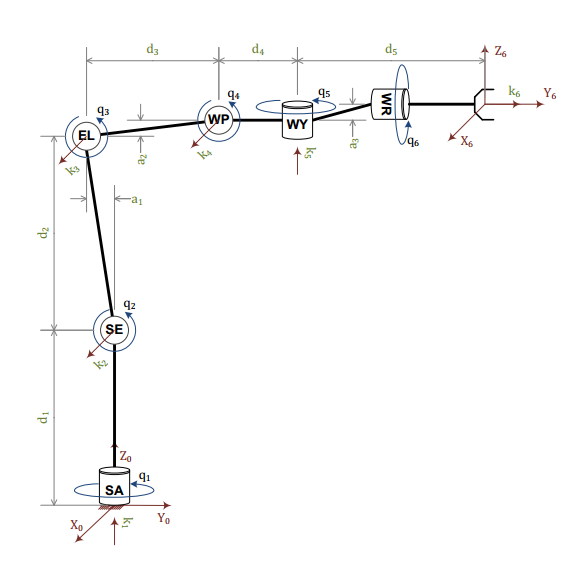
\includegraphics[scale=0.8]{FiguresP/DiagramaGrips}}
\subfigure{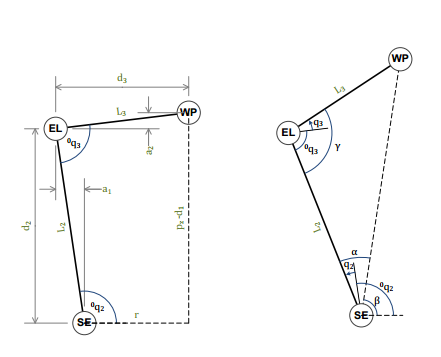
\includegraphics[scale=0.8]{FiguresP/DiagramaGrips2}}
\caption{Diagrama del Robot Grips}
\label{fig:diaGrips}
\end{figure}







%Given the special kinematic configuration of the MasterFinger 3, the use of the Denavit- Hartenberg convention [? ] would require dummy links to overcome the constraints that have to be met between coordinate frames. Specically, it would require a total of 14 joints for each finger when they only have 7.

%As an alternative, the displacement matrices approach proposed in [? ] can be used. This method can deal with any robot configuration without adding dummy links because it requires knowing the transformation (position and orientation) T0 of the robot end- efector at its home position (qi = 0 ∀ i), identifying the direction vector ki of the joint axis and selecting any point pi over the axis for all i.


También se presenta el método de matrices de desplazamiento \cite{barrientos2012modelado} como alternativa al método de Denavit y Hartenberg que puede trabajar sin la necesidad de añadir eslabones ficticios. Solo requiere conocer la transformación de la posición (posición y orientación) de $T_0$ del efector final del robot y su posición inicial, ($q_i=0 \forall i$), identificando la dirección del vector $\vec{k_i}$ del eje del eslabón y seleccionando algún punto $\vec{P_i}$ sobre el eje para todo $i$. Siendo $T_0$ la matriz de transformación, $q_i$ el i-\'esimo grado de libertad del robot y $\vec{k_i}$ el eje z del i-\'esimo eslabón. En el cuadro \ref{tab:dhslave} y en la figura 



%De manera similar al método de Denavit-Hartenberg \cite{hartenberg1964kinematic}, el método de matrices de desplazamiento
A continuación se presenta el algoritmo para encontrar el modelo cinemático directo usando matrices de desplazamiento.

\subsection{Modelo Cinemático Directo mediante Matrices de Desplazamiento}
\begin{itemize}
\item[D-1] Situando al robot en la posición cero ($q_i=0, \forall i$) encontrar la expresión de la matriz de transformación homogénea $T_0$ que localiza al extremo del robot referido al sistema de la base.

\item[D-2]
Para la misma posición del robot y para cada grado de libertad $q_i$ obtener la matriz de desplazamiento $D_i$, para ello:

\item[D-2.1]
    Identificar el vector unitario $\vec{k_i}$ del eje de la articulación expresado en las coordenadas del sistema de la base.

    

     \item[D-2.2] Seleccionar cualquier punto $\vec{P_i}$ del eje de la articulación

    \item[D-2.3] La matriz de desplazamiento asociada a ese grado de libertad, vendrá dada por\\
$$
D_i=\begin{pmatrix}
I & \vec{k_i}q_i\\
0 & 1
\end{pmatrix} 
$$
si el GDL es de traslación. O por\\
$$
D_i=\begin{pmatrix}
R_i & (I-R_i)\vec{p_i}\\
0 & 1
\end{pmatrix} 
$$
si el GDL es de rotación.\\

Siendo $I$ matriz identidad de dimensión 3 y la matriz $R_i$\\
\begin{center}


$R_i=I\cos{q_i}+\vec{k_i}\vec{k_i}^{T}(1-\cos{q_i})+skew(\vec{k_i})\sin{q_i}$\\
\end{center}
El operador \textbf{$skew$} es el que a cada vector $\vec{k}=(k_x,k_y,k_z)$ asocia la matriz antisimétrica.

$$skew(\vec{k})=\begin{pmatrix}
0 & -k_z & k_y\\
k_z & 0 & -k_x\\
-k_y & k_x & 0\\ 
\end{pmatrix}
$$
    
\item[D-3] El modelo cinemático directo \textsc{MCD} se tiene como el producto
$$
T_n=(\prod_{i=1}^n\mathbf{D_i})\mathbf{T_0}
$$

\end{itemize}

%\begin{algorithm}[H]  
% \KwData{situando al robot en la posición cero %($q_i=0, \forall i$) encontrar la expresión de la %matriz de transformación homogenea $T_0$ que se %localiza en el extremo del robot referido al sistema %de la base}
% \KwResult{how to write algorithm with \LaTeX2e }
% initialization\;
% \While{not at end of this document}{
%  read current\;
%  \eIf{understand}{
%   go to next section\;
%   current section becomes this one\;
%   }{
%   go back to the beginning of current section\;
%  }
% }
% \caption{Algoritmo para la obtención del modelo %cinemático del Robot mediante las Matrices de %Desplazamiento}
%\end{algorithm}


A continuación se presenta el código en Matlab que implementa lo anteriormente explicado.
\begin{lstlisting}
function T=MCD_MD (kk, pp, TO,tipo,n)
% kk(3,n) coordenadas del vector director del eje de la articulacion expresadas en {SO}, 
con el robot situado en qi=0
% pp(3,n) coordenadas de un punto del eje de la articulacion expresadas en {SO}, 
con el robot situado en qi=0
% TO (4,4) MTH del sistema de coordenadas del extremo {Sn} expresado en {SO},
 con el robot situado en cero qi = 0
% tipo(l,n) vale 0 si el gdl es de rotacion y 1 si es de traslacion
% n: numero de gdl
syms ql q2 q3 q4 q5 q6 real;
qq=sym([ql, q2, q3, q4, q5, q6]);
I=T0;
I=eye(3);
for i=n:-1:1
	k=kk (i,:)'; 	p=pp (i, :) ';q	=qq (i);
	if tipo(i)==0
		K=[0 -k(3) k(2);k(3) 0 -k(l);-k(2) ..
		k(l) 0];
		R=I*cos(q)+k*k'*(1-cos(q))+K*sin(q);
		D=[R, (I-R) *p; [0 0 0 1] ]
	else
		D=[eye (3) ,w*q; [0 0 0 1] ;
	end
I=simple(D*T);
end
end
 \end{lstlisting}  







\begin{table}[htb!]
\centering
\caption{Parámetros del método de matrices de desplazamiento para el robot GRIPS}
\label{tab:desplazamientoGrips}
\begin{tabular}{c c c}
\hline \\
Eje & Vector director $\vec{k_i}$ & Punto cualquiera en el eje de $\vec{P_i}$ \\
1				& $[0,0,1] $ &  $[0,0,0]$\\
2				& $[1,0,0] $ &  $[0,0,d_1]$\\
3				& $[1,0,0] $ &  $[0,-a_1,d_1+d_2]$\\
4				& $[1,0,0] $ &  $[0,-a_1+d_3,d_1+d_2+a_2]$\\
5				& $[0,0,1] $ &  $[0,-a_1+d_3+d_4,d_1+d_2+a_2]$\\
6				& $[0,1,0] $ &  $[-a_4,-a_1+d_3+d_4+d_5,d_1+d_2+a_2+d_3]$\\
\hline
\end{tabular}
\end{table}






En la ecuación \ref{eq:fkgrips} puede verse la matriz de desplazamiento para la cinemática directa del manipulador GRIPS y en la tabla \ref{tab:desplazamientoGrips} los valores a los que se hace referencia.
\begin{equation}
\label{eq:fkgrips}
T_0=\begin{pmatrix}
1 & 0 & 0 & -a_4\\
0 & 1 & 0 & -a_1+d_3+d_4+d_5\\
0 & 0 & 1 & d_1 +d_2+a_2+a_3\\
0 & 0 & 0 & 1  
\end{pmatrix}
\end{equation}

%Similar to the Denavit-Hartenberg  convention [? ], the displacement matrices method can be systematically implemented, see Algorithm 3.1. Placing the robot at its home position (qi = 0 ∀ i), and the homogeneous transformation T0 that locates the robot's end-efector reference frame relative to the base frame. In the same position and for each DoF qi obtain the displacement matrix Di : ˆ Identify the joint axis direction vector ki relative to the base frame. ˆ Select any point pi over the joint axis.



También puede utilizarse el método de matrices de desplazamiento en la obtención de la cinemática inversa, haciendo algunas simplificaciones para mantener expresiones mas claras:

$$
S_\theta=\sin\theta
$$

$$
C_\theta=\cos\theta
$$

$\mathbf{^{0}FK_{3}}$ La matriz de cinemática directa de los primeros tres GDL.

\begin{equation}
T_0=\begin{pmatrix}
1 & 0 & 0 & 0\\
0 & 1 & 0 & -a_1+d_3\\
0 & 0 & 1 & d_1+d_2+a_2\\
0 & 0 & 0 & 1  
\end{pmatrix}
\end{equation}


cuyos parametros pueden verse en la tabla \ref{tab:f3gdl}

\begin{table}[htb!]
\centering
\label{tab:f3gdl}
\caption{Parámetros del método de matrices de desplazamiento para los primeros tres GDL del robot GRIPS}
\begin{tabular}{c c c}
\hline \\
Eje & Vector director $\vec{k_i}$ & Punto cualquiera en el eje de $\vec{P_i}$ \\
1				& $[0,0,1] $ &  $[0,0,0]$\\
2				& $[1,0,0] $ &  $[0,0,d_1]$\\
3				& $[1,0,0] $ &  $[0,-a_1,d_1+d_2]$\\
\hline
\end{tabular}
\end{table}


obteniendo la siguiente matriz de transformación

%\begin{equation}
%^{0}T_3=\begin{pmatrix}
%c_1 & -c_{2+3} s_1  & s_{2+3}S_1   &  s_1(−d_3 c_{2+3} + a_2 s_{2+3} + a_1 c_2 + d_2 s_2 )\\
%s_1 &  c_{2+3} c_1  & -s_{2+3}C_1  & -c_1(-d_3 c_{2+3} + a_2 s_{2+3} + a_1 c_2 + d_2 s_2 )\\
%0   &  s_{2+3}      & c_{2+3}      & d_1 + a_2 c_{2+3} + d_3 s_{2+3} + d_2 c_2 + -a_1 s_2 \\
%0   &       0       &     0        &   1        
%\end{pmatrix}
%\end{equation}


Para los tre ultimos GDL (muñeca esferica) se tiene la matriz en la ecuación \ref{ec:fkwrist} $\mathbf{^{3}FK_6}$




\begin{equation}
\mathbf{T_0}=\begin{pmatrix}
1 & 0 & 0 & -a_4\\
0 & 1 & 0 & d_4+d_5\\
0 & 0 & 1 & a_3\\
0 & 0 & 0 & 1

\end{pmatrix}
\end{equation}



\begin{table}[htb!]
\centering
\label{tab:l3gdl}
\caption{Parámetros del método de matrices de desplazamiento para los últimos tres GDL del robot GRIPS}
\begin{tabular}{c c c}
\hline \\
Eje & Vector director $\vec{k_i}$ & Punto cualquiera en el eje de $\vec{P_i}$ \\
4				& $[1,0,0] $ &  $[0,0,0]$\\
5				& $[0,0,1] $ &  $[0,d_4,0]$\\
6				& $[0,1,0] $ &  $[-a_4,0,a_3]$\\
\hline
\end{tabular}
\end{table}


\begin{equation}
\label{ec:fkwrist}
\mathbf{^{6}T_3}=\begin{pmatrix}
n_x & o_x & a_x & p_x\\
n_y & o_y & a_y & p_y\\
n_z & o_z & a_z & p_z\\
0   & 0   & 0 & 1
\end{pmatrix}
\end{equation}




\begin{minipage}{0.9\textwidth}
\begin{tabular}{l l}


$n_x=C_5 C_6$ 				& \hspace{2cm} $a_x=C_5 S_6$\\
$n_y=S_4 S_5 +  C_4 C_6 S_5$	& \hspace{2cm} $a_y=-C_6 S_4 + C_4 S_5 S_6$\\
$n_z=-C_4 S_6 + C_6 S_4 S_5$ & \hspace{2cm} $a_z=C_4 C_6 + S_4 S_5 S_6$\\
$o_x=-S_5$ 					& \hspace{2cm} $p_x=-a_4 C_5 -d_5 S_5$\\
$o_y=C_4 C_5$ 				& \hspace{2cm} $p_y=d_4 C_4 -a_3 S_4 + d_5 C_4 C_5 -a_4 C_4 S_5$\\
$o_z=C_5 S_4$ 				& \hspace{2cm} $p_z=a_3 C_4 d_4 S_4  + d_5 C_5 S_4 -a_4 S_4 S_5$\\
\end{tabular}
\end{minipage}








%%A continuación se muestran las matrices de rotación y traslación que corresponden al robot planar de dos grados de libertad. Para obtener las coordenadas cartesianas hay que multiplicar las matrices de trasformación homogénea y evaluarlas en los puntos de las coordenadas articulares.\\
%
%
%\begin{eqnarray}
%R_{0}^{1}=\begin{pmatrix}
%\cos q_1 &  -\sin q_1 & 0 & 0\\
%\sin q_1 &   \cos q_1 & 0 & 0\\
%0        & 0          & 1 & 0\\
%0        & 0          & 0 & 1
%\end{pmatrix} \\ 
%T_{0}^{1}=\begin{pmatrix}
%1 & 0 & 0 & l1\cos(q1)\\
%0 & 1 & 0 & l1\sin(q1)\\
%0 & 0 & 1 & 0\\
%0 & 0 & 0 & 1
%\end{pmatrix} \\
%R_{1}^{2}=\begin{pmatrix}
%\cos q_2 &  -\sin q_2 & 0 & 0\\
%\sin q_2 &   \cos q_2 & 0 & 0\\
%0        & 0          & 1 & 0\\
%0        & 0          & 0 & 1
%\end{pmatrix} \\ 
%T_{1}^{2}=\begin{pmatrix}
%1 & 0 & 0 & l2\cos(q2)\\
%0 & 1 & 0 & l2\sin(q2)\\
%0 & 0 & 1 & 0\\
%0 & 0 & 0 & 1
%\end{pmatrix} \\
%A_0^{2}=R_0^{1} T_0^{1} R_1^{2} T_1^{2} 
%\end{eqnarray}
%
%Para  calcular la cinemática directa se introducen en un \textbf{Script de MATALB} las matrices de traslación y rotación del mecanismo, y se proponen valores para $q_1,l_1 $ y $q_2,l_2 $ , como se puede ver a continuación:
%\begin{verbatim}
%q1=30;
%q2=45;
%l1=1;
%l2=1;
%t1=[[1 0 0 l1*cosd(q1)]
%    [0 1 0 l1*sind(q1)]
%    [0 0 1 0]
%    [0 0 0 1]]
%
%t2=[[cosd(q1) -sind(q1) 0 0]
%    [sind(q1) cosd(q1)  0 0]
%    [0 0 1 0]
%    [0 0 0 1]]
%
%
%t3=[[1 0 0 l2*cosd(q2)]
%    [0 1 0 l2*sind(q2)]
%    [0 0 1 0]
%    [0 0 0 1]]
%
%
%t4=[[cosd(q2) -sind(q2) 0 0]
%    [sind(q2) cosd(q2)  0 0]
%    [0 0 1 0]
%    [0 0 0 1]]
%\end{verbatim}
%Después podemos resolver el problema mediante el método de Denavit Hartenberg solo para comprobar nuestro resultado:
%
%\begin{tabular}{|c|c|c|c|c|}
%
%\hline 
%Articulación & $\theta$ & d & a & $\alpha$ \\ 
%\hline 
%1 & $q_1$ & 0 & $l_1$ & 0 \\ 
%\hline 
%2 & $q_2$ & 0 & $l_2$ & 0 \\ 
%\hline 
%\end{tabular} 


%
%
%\begin{verbatim}
%a01=[[cosd(q1) -sind(q1) 0 l1*cosd(q1)]
%    [sind(q1) cosd(q1) 0 l1*sind(q1)]
%    [0 0 1 0]
%    [0 0 0 1]]
%
%
%a12=[[cosd(q2) -sind(q2) 0 l2*cosd(q2)]
%    [sind(q2) cosd(q2) 0 l2*sind(q2)]
%    [0 0 1 0]
%    [0 0 0 1]]
%    
%T=t1*t2*t3*t4
%dh=a01*a12
%\end{verbatim}
%
%
%Como resultado tenemos:
%\begin{verbatim}
%T = 0.2588   -0.9659         0    1.1248
%    0.9659    0.2588         0    1.4659
%         0         0    1.0000         0
%         0         0         0    1.0000
%
%
%dh =0.2588   -0.9659         0    1.1248
%    0.9659    0.2588         0    1.4659
%         0         0    1.0000         0
%         0         0         0    1.0000
%
%\end{verbatim}
%Podemos observar el mismo resultado con lo que se concluye que se ha efectuado el procedimiento de  manera correcta. Se muestra también una representación gráfica del mecanismo en la figura


\subsection{Cinemática inversa}
Se tiene el siguiente conjunto de ecuaciones obtenidas del la figura \ref{fig:diaGrips} , las cuales describen las coordenadas articulares del robot, a partir de un punto dado en el espacio mediante relaciones geométricas simples para los tres primeros grados de libertad.

\begin{eqnarray}
 q_1=\arctan{\frac{P_y}{P_x}} \\ 
 r^{2}=P_x^{2}+P_y^{2}\\ 
 r^{2}=+P_2^{2}=l_2^{2}+l_3^{2}+l_2l_3\cos{q_3}\\ 
 \cos{q_3}=\frac{P_x^{2}+P_y^{2}+P_2^{2}-l_2^{2}-l_3^{2}}{2l_2l_3}\\ 
 \sin{q_3}=\sqrt{1-\cos^{2}{q_3}}\\ 
 q_3=\arctan{\frac{\sqrt{1-\cos^{2}{q_2}}}{\cos{q_3}}}\\ 
 q_2=\beta -\alpha\\ 
 \beta=\arctan{\frac{P_z}{r}}=\arctan{\frac{P_z}{\sqrt{P_x^{2}+P_y^{2}}}}\\ 
 \alpha=\arctan{\frac{l_2\sin{q_3}}{l_2+l_3 \cos{q_3}}}\\ 
 q_2=\arctan{\frac{P_z}{\sqrt{P_z^{2}}+P_y^{2}}}-\arctan{\frac{l_3\sin{q_3}}{l_2+l_3\cos{q_3}}}
\end{eqnarray}
Se observa que en la cinemática inversa pueden existir soluciones alternas. Debido a esto usamos la función \textbf{atan2} la cual nos arroja solo una de las posibles soluciones.\\
 
 
Para el caso de la orientación del efector final se tienen las siguientes ecuaciones obtenidas a partir de la ecuación \ref{ec:fkwrist} 




%La siguiente función en MATLAB recibe como entrada las coordenadas cartesianas del efector final del robot y devuelve las coordenadas articulares.
%\subsection{Desplazamiento lineal}
%Se creo la siguiente función en MatLab para el robot de dos grados de libertad
%\begin{verbatim}
%function Y=dosgdl(l2, l3, py, px)
%Cq3=(px^2+py^2-l2^2-l3^2)/(2*l2*l3)
%Sq3= sqrt(1-((Cq3)^2))
%q3= atand(Sq3/Cq3)
%Betha = atand(py/px)
%Alfa = atand((l3*sind(q3))/(l2+(l3*Cq3)))
%q2=Betha-Alfa
%%x2=[0 l2*cosd(q2)]
%%y2=[0.5 l2*sind(q2)]
%x3=[0 l2*cosd(q2) l3*cosd(q3+q2)+l2*cosd(q2)]
%y3=[0 l2*sind(q2) l3*sind(q3+q2)+l2*sind(q2)]
%Y=[x3;y3]
%%line(x2, y2);
%line(x3, y3);
%axis([0 5 0 5]); 
%\end{verbatim}
%
%
%
%
%Posteriormente se varía la trayectoria a seguir por el robot usando un ciclo for
%\begin{verbatim}
%clc, clear, close all
%l2=2;
%l3=1;
%xt=[];
%yt=[];
%px= []
%py= 2;
%for px=1:0.1:2.2
%
%Y= dosgdl(l2, l3, py, px);
%xt= Y(1);
%yt= Y(2);
%drawnow;
%pause(0.1);
%clf;
%end
%\end{verbatim}
%



















%\newpage
%\subsection{Ecuaciones dinámicas}
%Podemos modelar este sistema como un péndulo doble ver figura  en general el péndulo doble es un sistema compuesto por dos péndulos, con el segundo extremo colgando del primero, asumimos que se trata de dos péndulos simples, este sistema físico posee dos grados de libertad. su movimiento está gobernado por dos ecuaciones diferenciales ordinarias acopladas. Cabe mencionar que por encima de cierta energía el sistema es caótico. Para el modelado del sistema usamos el método de \textbf{Euler-Lagrange}, como se muestra a continuación.

%\subsection{Energía}
%
%La energía cinética puede expresarse como:
%\begin{eqnarray}
%T=\frac{1}{2}m_1(\dot{x}_1^{2}+\dot{y}_1^{2})+\frac{1}{2}m_2(\dot{x}_2^{2}+\dot{y}_2^{2})\\
%=\frac{1}{2}m_1 l_1^{2}\dot{\theta}_1^{2}+\frac{1}{2}m_2(l_1^{2}\dot{\theta}_1^{2}+l_2^{2}\dot{\theta}_2^{2} + 2l_1^{2} l_2^{2}\dot{\theta}_1^{2} \dot{\theta}_2^{2} \cos{(\theta_1-\theta_2)})
%\end{eqnarray}
%
%La energía potencial:
%\begin{eqnarray}
%V=m_1 g y_1 + m_2 g y_2\\
%=-(m_1 + m_2)gl_1 \cos\theta_1 -m_2gl_2 \cos\theta_2
%\end{eqnarray}
%Tenemos que la siguiente ecuación  según \textbf{Lagrange} es:
%\begin{equation}
%L=T-V
%\end{equation}
%Sustituyendo la energía cinética y potencial en la ecuación de \textbf{Lagrange} tenemos:
%\begin{equation}
%L=\frac{1}{2}m_1 l_1^{2}\dot{\theta}_1^{2}+\\
% \frac{1}{2}m_2(l_1^{2}\dot{\theta}_1^{2}+l_2^{2}\dot{\theta}_2^{2} + 2l_1^{2} l_2^{2}\dot{\theta}_1^{2} \dot{\theta}_2^{2} \cos{(\theta_1-\theta_2)})+(m_1 + m_2)gl_1 \cos\theta_1 +m_2gl_2 \cos\theta_2
%\label{lagrangiano}
%\end{equation}
%
%A partir de la ecuación \ref{lagrangiano} podemos obtener la ecuación del movimiento a partir de las ecuaciones \ref{l1} y \ref{l2}:
%
%\begin{eqnarray}
%\frac{d}{dt}(\frac{\partial L}{\partial \dot{\theta}_1})-\frac{\partial L}{\partial \theta_1 } \label{l1}\\ 
%\frac{d}{dt}(\frac{\partial L}{\partial \dot{\theta}_2})-\frac{\partial L}{\partial \theta_2 } \label{l2}
%\end{eqnarray}
%
%\begin{flushleft}
%{ \fboxsep 12pt
%
%\begin{minipage}[t]{18cm}
%
%Haciendo las correspondientes derivadas parciales y ordinarias llegamos a las ecuaciones de movimiento:
%
%\begin{align}
%(m_1+m_2)l_1^{2} \ddot{\theta}_1+ m_2\ddot{\theta}_2 l_1 l_2 \cos{(\theta_1-\theta_2)}-m_2\dot{\theta}_2 l_1 l_2(\theta_1 - \theta_2)\sin{(\theta_1-\theta_2)} +m_2\dot{\theta}_1 \dot{\theta}_2 l_1 l_2 \sin{(\theta_1 -\theta_2)}+ (m_1 + m_2) gl_1\sin{\theta_1} =0\\
%m_2l_2^{2}\ddot{\theta}_2 + m_2\ddot{\theta}_1 l_1 l_2 \cos{(\theta_1 - \theta_2)} -m_2 \dot{\theta}_1 l_1 l_2(\dot{\theta}_1-\dot{\theta}_2)\sin{(\theta_1-\theta_2)} -m_2\dot{\theta}_1\dot{\theta}_2 l_1 l_2 \sin{(\theta_1- \theta_2)}+m_2gl_2\sin \theta_2= 0
%\end{align}
%\end{minipage}
% }
%\end{flushleft}




\newpage
\subsection{Espacio de Trabajo}

En la figura \ref{fig:gripsworkspace} se muestra el espacio de trabajo del manipulador esclavo GRIPS


\begin{figure}[htb!]
\subfigure[\'Area de trabajo en el plano XZ del robot esclavo]{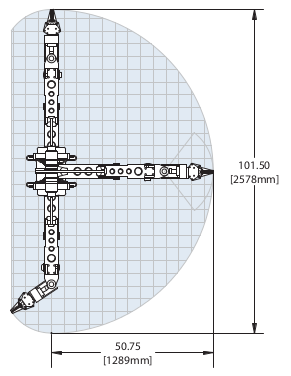
\includegraphics[scale=0.5]{FiguresP/grips6}}
\subfigure[\'Area de trabajo en el plano XY del robot esclavo]{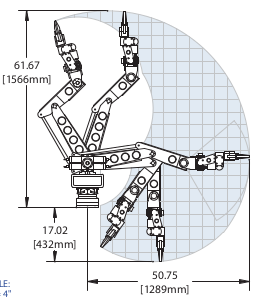
\includegraphics[scale=0.6]{FiguresP/grips5}}
\subfigure[Robot esclavo GRIPS]{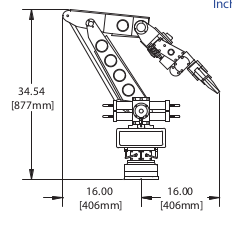
\includegraphics[scale=0.6]{FiguresP/grips1}}
\caption{Espacio de trabajo del robot esclavo Grips}
\label{fig:gripsworkspace}
\label{RobotGrips}
\end{figure}


\section{Señales del Robot Esclavo}
En la tabla \ref{tab:signalsSlave} se describen las señales del manipulador esclavo.
\begin{sidewaystable}[htbp]
  \centering
  \caption{Listado de señales del robot esclavo}
    \begin{tabular}{lllccccc}
    \toprule
    \multicolumn{1}{c}{\multirow{2}{*}{\textbf{TAG}}} & \multicolumn{1}{c}{\multirow{2}{*}{\textbf{ORIGEN}}} & \multicolumn{1}{c}{\multirow{2}{*}{\textbf{DESCRIPCIÓN}}} & \multicolumn{1}{c}{\multirow{2}{*}{\textbf{TIPO SEÑAL}}} & \multicolumn{4}{c}{\textbf{SEÑAL}} \\  
  &  &  & & \textbf{DI} & \textbf{DO} & \textbf{AI} & \textbf{AO} \\
    \midrule
  	SLA-VSA & Esclavo, Servo-Valvula SA & Salida Analógica, $\pm$10V, 200mA & Comando &       &       &       & 1 \\
    SLA-VSE & Esclavo, Servo-Valvula SE & Salida Analógica, $\pm$10V, 200mA & Comando &       &       &       & 1 \\
    SLA-VEL & Esclavo, Servo-Valvula EL & Salida Analógica, $\pm$10V, 200mA & Comando &       &       &       & 1 \\
    SLA-VWY & Esclavo, Servo-Valvula WY & Salida Analógica, $\pm$10V, 200mA & Comando &       &       &       & 1 \\
    SLA-VWP & Esclavo, Servo-Valvula WP & Salida Analógica, $\pm$10V, 200mA & Comando &       &       &       & 1 \\
    SLA-VWR & Esclavo, Servo-Valvula WR & Salida Analógica, $\pm$10V, 200mA & Comando &       &       &       & 1 \\
    SLA-VGRIP & Esclavo, Servo-Valvula Gripper & Salida Analógica, $\pm$10V, 200mA & Comando &       &       &       & 1 \\
    SLA-PSA & Esclavo, Potenciómetro SA & Valor de Voltaje $\pm$10V & Medida &       &       & 1     &  \\
    SLA-PSE & Esclavo, Potenciómetro SE & Valor de Voltaje $\pm$10V & Medida &       &       & 1     &  \\
    SLA-PEL & Esclavo, Potenciómetro EL & Valor de Voltaje $\pm$10V & Medida &       &       & 1     &  \\
    SLA-PWP & Esclavo, Potenciómetro WP & Valor de Voltaje $\pm$10V & Medida &       &       & 1     &  \\
    SLA-PWY & Esclavo, Potenciómetro WY & Valor de Voltaje $\pm$10V & Medida &       &       & 1     &  \\
    SLA-PWR & Esclavo, Potenciómetro WR & Valor de Voltaje $\pm$10V & Medida &       &       & 1     &  \\
    SLA-TSA & Esclavo, Transductor SA & Valor de Voltaje $\pm$10V & Medida &       &       & 1     &  \\
    SLA-TSE & Esclavo, Transductor SE & Valor de Voltaje $\pm$10V & Medida &       &       & 1     &  \\
    SLA-TEL & Esclavo, Transductor EL & Valor de Voltaje $\pm$10V & Medida &       &       & 1     &  \\
    SLA-TWP & Esclavo, Transductor WP & Valor de Voltaje $\pm$10V & Medida &       &       & 1     &  \\
    SLA-TWY & Esclavo, Transductor WY & Valor de Voltaje $\pm$10V & Medida &       &       & 1     &  \\
    SLA-TGR & Esclavo, Transductor GR & Valor de Voltaje $\pm$10V & Medida &       &       & 1     &  \\
    SLA-HYD & Esclavo, Solenoide Principal & Electroválvula, +24V, 1A & Comando &       & 1     &       &  \\
    \midrule
    \multicolumn{4}{r}{\textbf{TOTAL}} & 0 & 1 & 12 & 7 \\
    \bottomrule
    \end{tabular}%
  \label{tab:signalsSlave}%
\end{sidewaystable}%








































\newpage
\section{Sistema Maestro}

\begin{figure}[htb!]
\centering
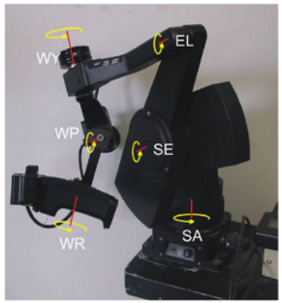
\includegraphics[scale=0.95]{FiguresP/Maestro}
\caption{Manipulador Maestro }
\label{fig:maestro}
\end{figure}

El robot maestro (ver figura \ref{fig:maestro}) es cinemáticamente similar al robot esclavo. Tiene tres grados de libertad para determinar la posición de la muñeca y tres m\'as para determinar su orientación. Como sensores de posición angular el sistema maestro cuenta con potenci\'ometros en cada una de las seis articulaciones. Las cinco primeras son actuadas eléctricamente para reflejar las fuerzas ejercidas en el robot esclavo. La pinza puede controlarse de manera proporcional pero sin realimentación por medio de un potenciometro. También cuenta con distintos botones para activar funciones como la rotación continua de la muñeca, bloqueo de la pinza y bloquear y continuar en la posición del esclavo y maestro.\\

Un botón ubicado en la base del maestro controla el encendido del sistema hidráulico, en el antebrazo  se encuentran tres LED que indican el estado de bloqueo de la pinza (\textit{Grip lock}), el modo de rotación de la muñeca (\textit{Cont wrist}), y el bloqueo de la posición del sistema (\textit{Halt}). Un LED ubicado al lado del botón para encender la hidráulica indica su estado (ver figura \ref{fig:leds}).



\begin{figure}[htb!]
\centering

\subfigure[Leds indicadores de estado]{
\includegraphics[scale=0.1]{FiguresP/leds}\label{fig:leds}}
\subfigure[Pulsador de hidráulica on/off]{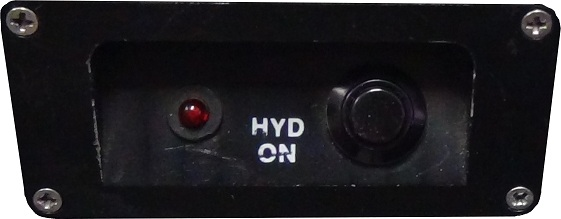
\includegraphics[scale=0.3]{FiguresP/PulsadorHyd}\label{fig:pulsadorhid}}
\subfigure[Detalle de la muñeca del dispositivo maestro]{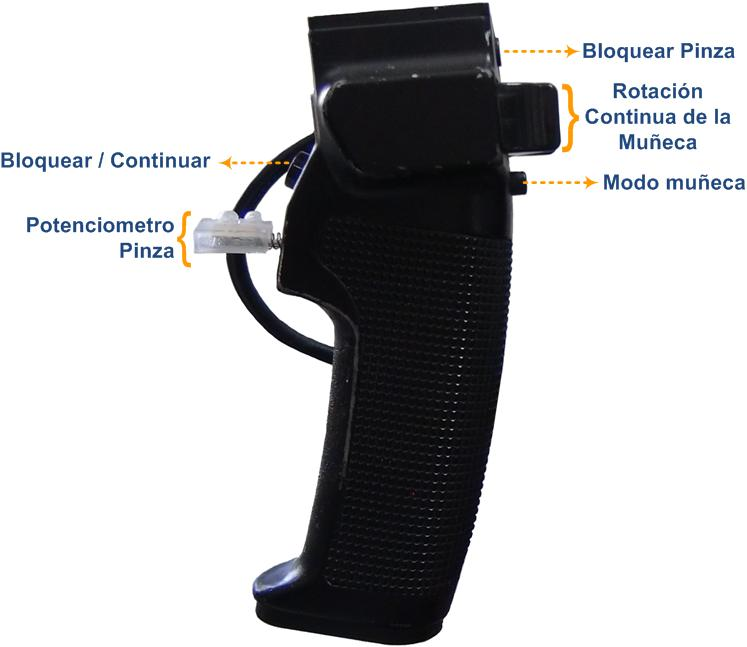
\includegraphics[scale=0.4]{FiguresP/Pulsadores}\label{fig:muñeca}}
\caption{Botones, LED y potenci\'ometros del maestro GRIPS}
\label{fig:leds}
\end{figure}








\newpage
\subsection{Sensores y Actuadores}

\begin{figure}[hbt!]
\centering
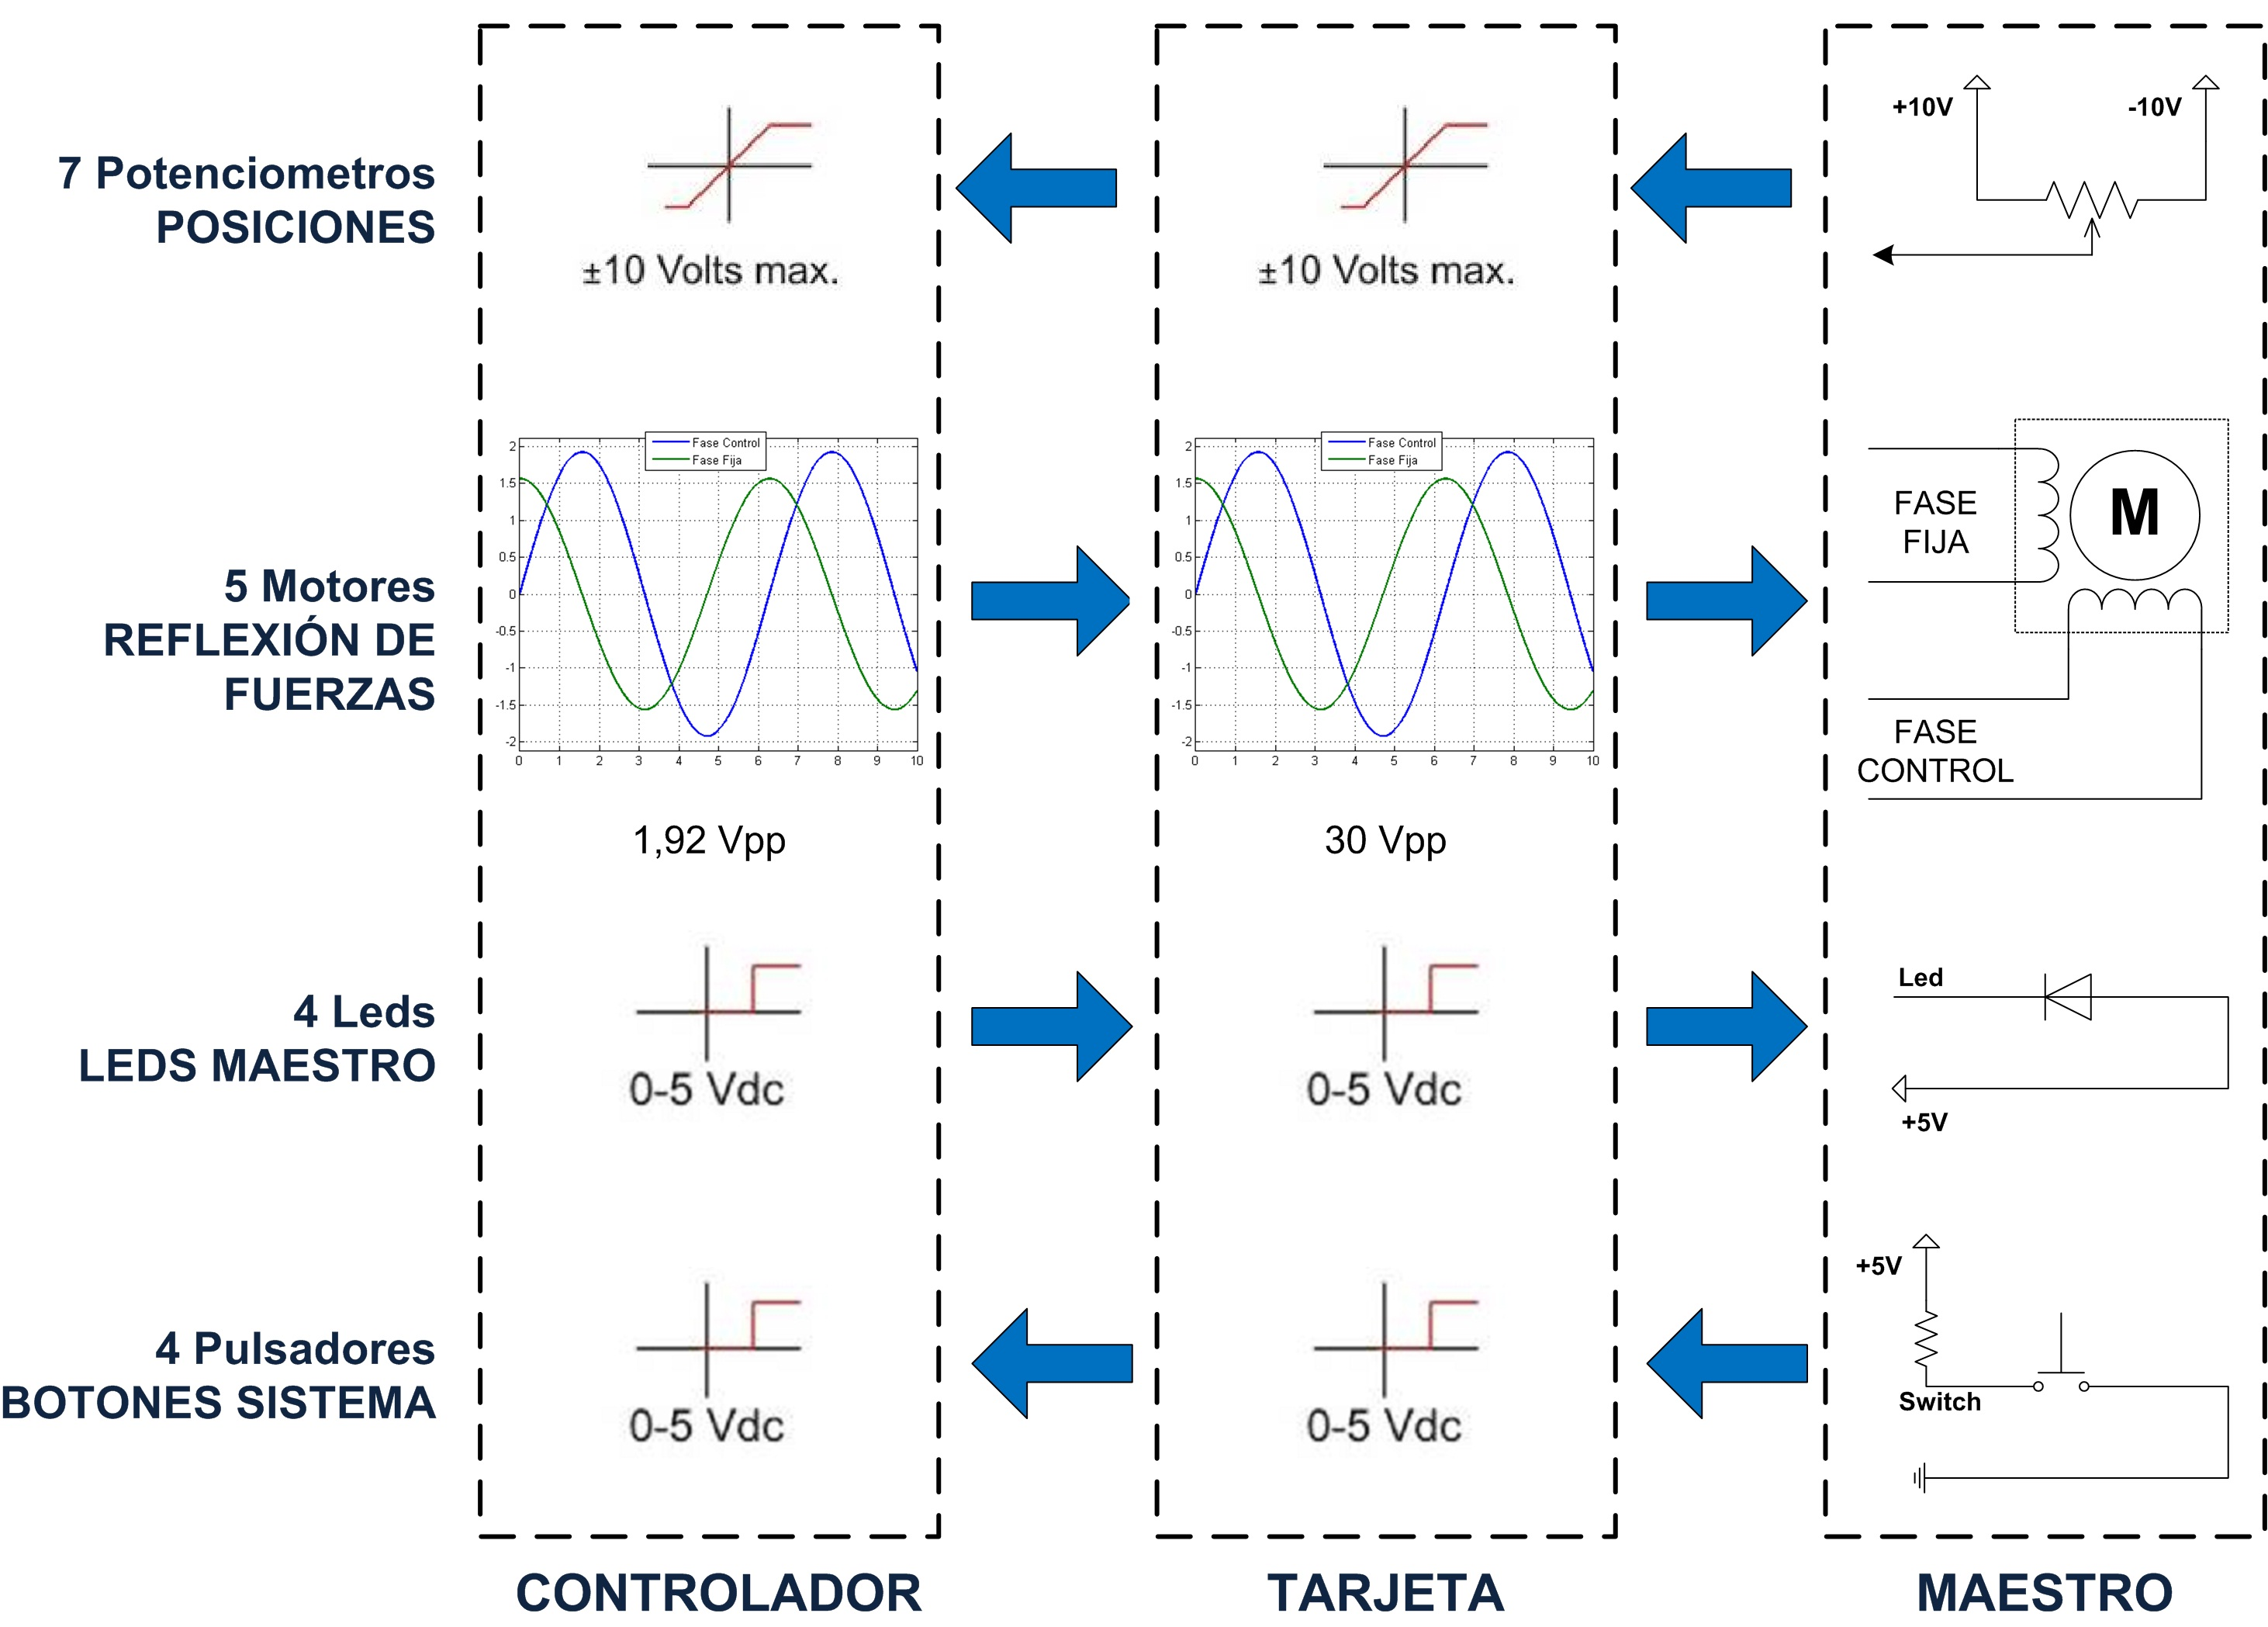
\includegraphics[scale=0.2]{FiguresP/EsquemaMaestroCard}
\caption{Tarjeta para Mediciones de Corriente}
\label{fig:TarjetaCorriente}
\end{figure}

\subsection*{Sensores}
El sistema maestro al igual que el sistema esclavo cuenta con poteni\'ometros para determianr las posiciones angulares de las articulaciones.




\subsection*{Actuadores}
Como puede observarse en la figura \ref{fig:motores}, el dispositivo maestro cuenta con cinco motores bif\'asicos de corriente alterna para realimentar la fuerza ejercida en el entorno remoto al operador. Para accionarlos son necesarias dos señales de corriente alterna(ver figura \ref{fig:señales}) que son generadas por el controlador de tiempo real y posteriormente amplificadas en una etapa de potenciab(ver figura \ref{fig:TarjetaMaestro}).  El sentido de rotación del motor depende de si la fase de control est\'a en adelanto o en atraso respecto a la fase fija. El par ejercido depende de la amplitud de ambas ondas.


\begin{figure}[htb!]
\centering
\subfigure[Señales de control para los motores del dispositivo maestro]{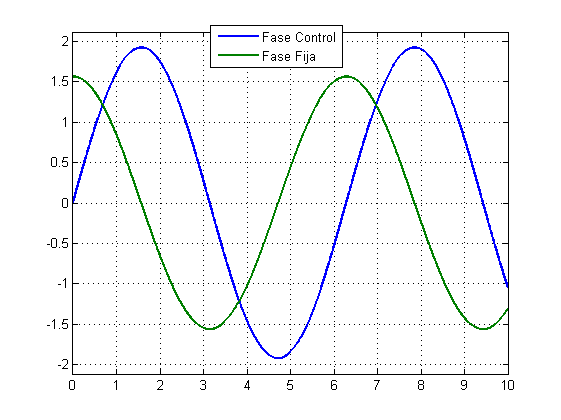
\includegraphics[scale=0.4]{FiguresP/entradaMotores}\label{fig:señales}}
\subfigure[Motores bifasicos utilizados para la realimentacion de fuerzas al operador]{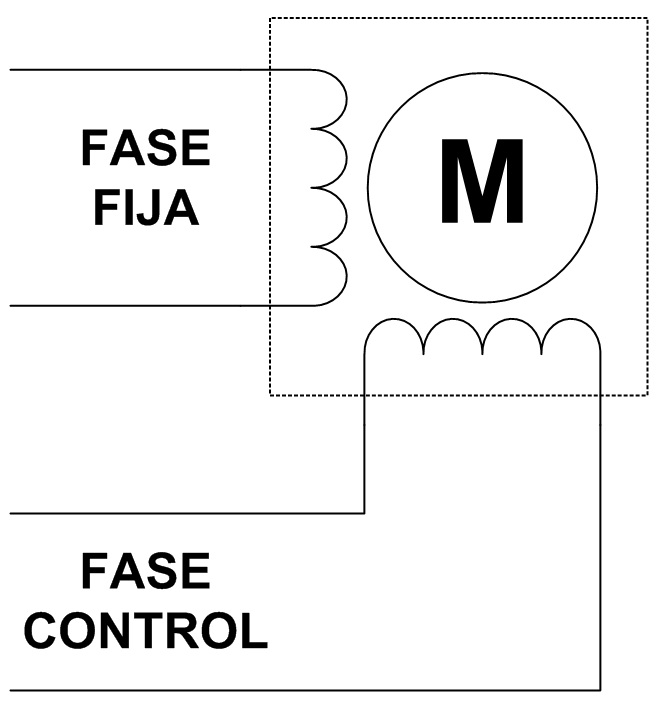
\includegraphics[scale=0.2]{FiguresP/MotorBifasico}\label{fig:motores}}
\caption{Esquema de los actuadores usados en el dispositivo maestro}
\end{figure}





\section*{Electrónica de Potencia}
Las señales de control son amplificadas en el circuito de la figura \ref{fig:etapaPotencia}.
\begin{figure}[htb!]
\centering
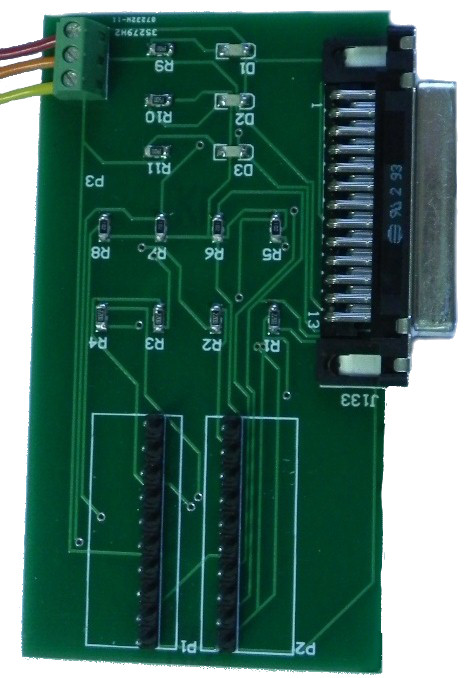
\includegraphics[scale=0.9]{FiguresP/TarjetaMaestro}
\caption{Tarjeta de entradas/salidas digitales y analógicas }
\label{fig:TarjetaMaestro}
\end{figure}


P

\begin{figure}[htb!]
\centering
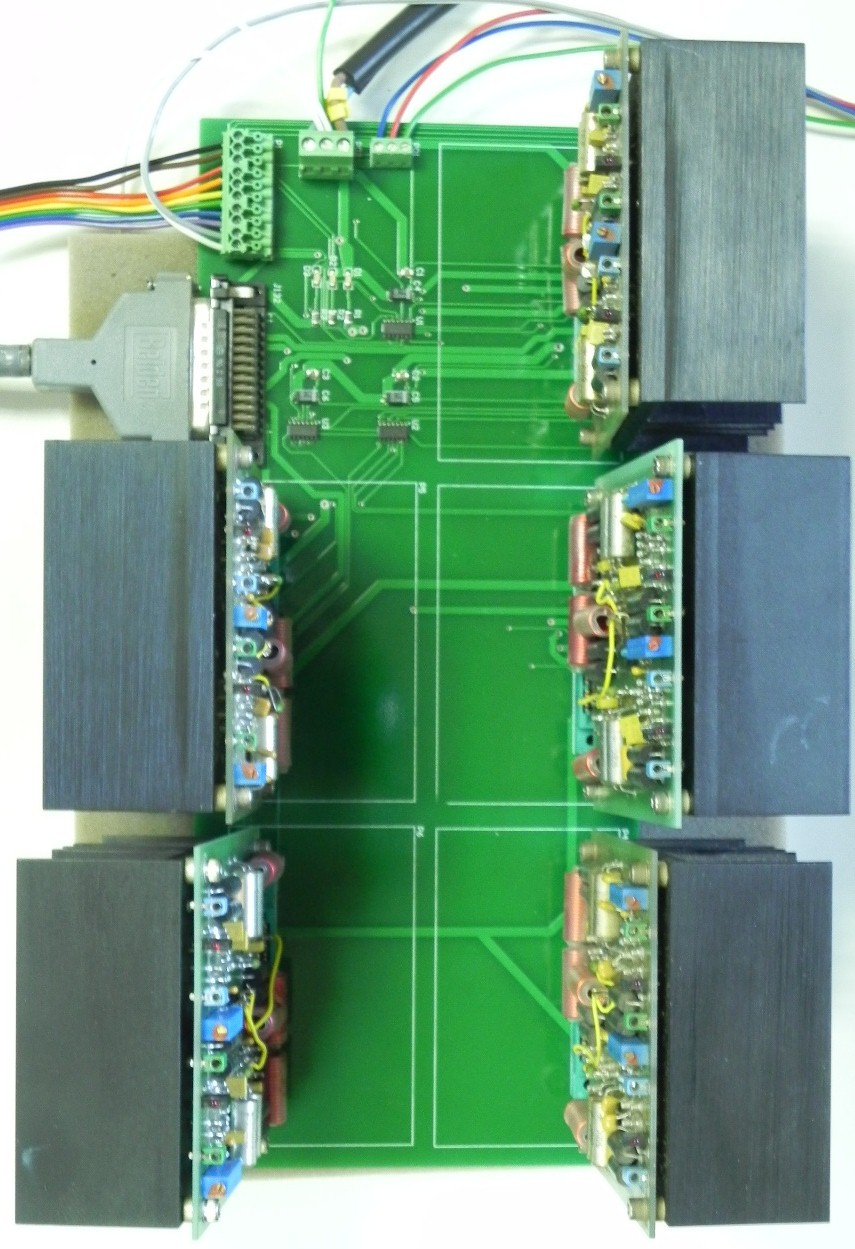
\includegraphics[scale=0.6]{FiguresP/TarjetaMotores}
\caption{Etapa de potencia de los motores}
\label{fig:etapaPotencia}
\end{figure}










%\subsection{Modelo Cinemático y Parámetros D-H}
%\begin{table}[]
%\centering
%\begin{tabular}{|c|c|c|c|c|}
% \hline
% \hline
% Articulación & $a_1$ & $\alpha_i$ & $d_i$ & $\theta_i$ \\
% \hline
% \hline
% 1 & 0      & $\frac{\pi}{2}$  & 0     & $\theta_1$\\
% 2 & $a_2$  & 0                & 0     & $\theta_1$\\
% 3 & 0      & $\frac{\pi}{2}$  & 0     & $\theta_1$\\
% 4 & 0      & $\frac{-\pi}{2}$ & $d_3$ & $\theta_1$\\
% 5 & 0      & $\frac{\pi}{2}$  & 0     & $\theta_1$\\
% 6 & 0      & 0                & $d_6$ & $\theta_1$\\
% \hline
% \hline
%\end{tabular}
%\caption{Parámetros D-H}
%\label{tab:MCD}
%\end{table}


%\subsection{Ecuaciones dinámicas}
%El Formalismo Lagrangiano presenta varias ventajas  en comparación con el método de Newton-Euler como lo son la fácil compresnión, ademas las matrices de inercia







%\subsection{Modelo Cinemático Inverso}



%\subsection{Espacio de Trabajo}





%Para el control LabView lenguaje gráfico de programación que permite 

%LabVIEW (acrónimo de Laboratory Virtual Instrumentation Engineering Workbench) es una plataforma y entorno de desarrollo para diseñar sistemas, con un lenguaje de programación visual gráfico. Recomendado para sistemas hardware y software de pruebas, control y diseño, simulado o real y embebido, pues acelera la productividad. El lenguaje que usa se llama lenguaje G, donde la G simboliza que es lenguaje Gráfico.

%Este programa fue creado por National Instruments (1976) para funcionar sobre máquinas MAC, salió al mercado por primera vez en 1986. Ahora está disponible para las plataformas Windows, UNIX, MAC y GNU/Linux. La última versión es la 2013, con la increíble demostración de poderse usar simultáneamente para el diseño del firmware de un instrumento RF de última generación, a la programación de alto nivel del mismo instrumento, todo ello con código abierto.

%Los programas desarrollados con LabVIEW se llaman Instrumentos Virtuales, o VIs, y su origen provenía del control de instrumentos, aunque hoy en día se ha expandido ampliamente no sólo al control de todo tipo de electrónica (Instrumentación electrónica) sino también a su programación embebida, comunicaciones, matemáticas, etc. Un lema tradicional de LabVIEW es: "La potencia está en el Software", que con la aparición de los sistemas multinúcleo se ha hecho aún más potente. Entre sus objetivos están el reducir el tiempo de desarrollo de aplicaciones de todo tipo (no sólo en ámbitos de Pruebas, Control y Diseño) y el permitir la entrada a la informática a profesionales de cualquier otro campo. LabVIEW consigue combinarse con todo tipo de software y hardware, tanto del propio fabricante -tarjetas de adquisición de datos, PAC, Visión, instrumentos y otro Hardware- como de otros fabricantes.









\section{Controlador en Tiempo Real }

La plataforma de teleoperación es gobernada mediante un controlador en tiempo real de National Instruments NI PXIe-1078 (figura \ref{fig:pxi_ebedded_controller}) con módulos de adquisición de datos que leen las señales provenientes de los sensores de posición y de fuerza.\\



El módulo NI PXIe-1078 consiste en un chásis de nueve ranuras, junto con una ranura para un controlador que puede ser embebido o remoto.\\


El chasis PXI incorpora un controlador de tiempo real NI PXIe-8182 de doble núcleo con una frecuencia de operación de 1.9 GHZ funcionando con VxWorks. Las fuerzas de interacción provienen del entorno remoto  a través de internet mediante el protocolo UDP.\\

El controlador es usado para realizar cálculos complejos (jacobiana, ecuaciones cinemáticas, ecuaciones de control, entre otras) que transforman la fuerza de interacción en los valores deseados en los actuadores y también para calcular la posición $(x,y,z)$ y la orientación \textsc{(Roll, Pitch, Yaw )}.


%\begin{figure}
%\centering
%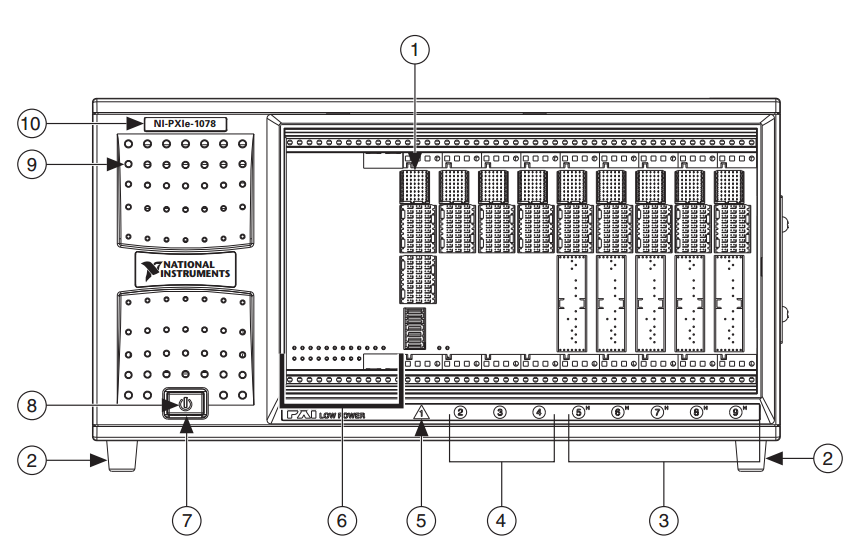
\includegraphics[scale=0.4]{FiguresP/pxi}
%\caption{NI PXIe-1078}
%\label{fig:pxi}
%\end{figure}


\begin{figure}[htb!]
\centering
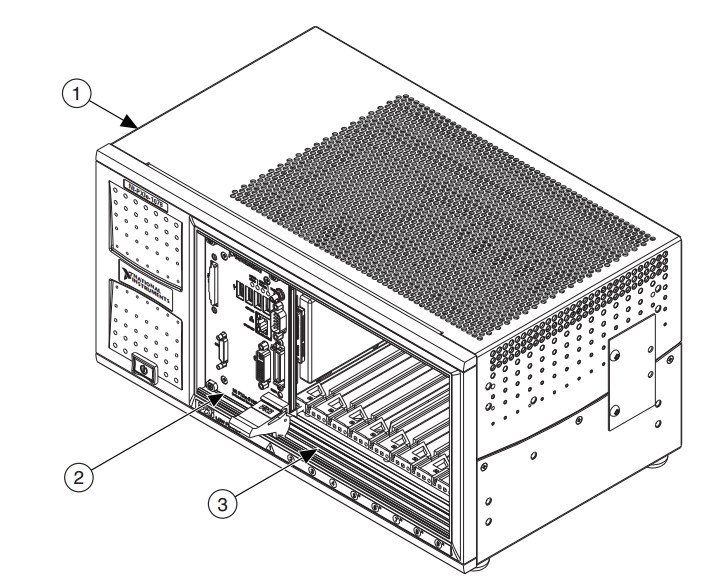
\includegraphics[scale=0.4]{FiguresP/pxi2}
\caption{NI PXIe-1078 con su controlador embebido}
\label{fig:pxi_ebedded_controller}
\end{figure}



El sistema NI PXIe-1078 con el que se está trabajando tiene las siguientes especificaciones:
\begin{itemize}
\item 5 ranuras híbridas, 3 ranuras PXI Express
\item 300 W de potencia total disponible desde 0 a 50 ºC
\item Rendimiento medio - Ancho de banda hasta250 MB/s por ranura y ancho de banda del sistema de 1 GB/s
\item Chasis de poca profundidad de 8.43 in. (214.2 mm) 
\item Compatibilidad con módulos PXI, PXI Express, CompactPCI y CompactPCI Express
\end{itemize}






%The NI PXIe-1078 chassis kits consist of a low-cost, 9-slot chassis featuring a 4-slot-wide system controller slot, which can accept either an embedded controller or remote controller, and eight peripheral slots. The NI PXIe-1078 offers the flexibility to populate each peripheral slot with a PXI Express module or populate up to five slots with PXI modules. In addition, it features compact, rugged packaging, and quiet operation, which make it ideal for portable, desktop, and industrial control applications






\subsection*{Módulo de adquisición de datos NI PXIe-6363 (figura \ref{fig:daq})}

\begin{itemize}
\item 32 entradas analógicas, 2 MS/s monocanal, 1.25 MS/s multicanal, resolución de 16 bits, $\pm$ 10 V
\item Cuatro salidas analógicas, 2.86 MS/s, resolución de16 bits, $\pm$ 10 V
\item 48 líneas de E/S digital (32 temporizadas por hardware hasta 10 MHz)
\item Cuatro contadores/temporizadores de 32 bits para PWM, codificador, contar eventos y más
\item Disparo analógico y digital y temporización 
\item Soporte para Windows 7/Vista/XP/2000
\end{itemize}



\begin{figure}[htb!]
\centering
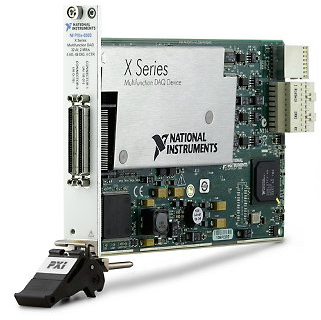
\includegraphics[scale=0.5]{FiguresP/pxi6363}
\caption{Módulo de adquisición de datos NI PXIe-6363}
\label{fig:daq}
\end{figure}


Para conectar los modulos de adquisicion de datos con las señales provenientes de los sensores se usa un m\'odulo de conexiones como el que se muestra en la figura \ref{fig:conexionPXI}.



\begin{figure}[htb!]
\centering
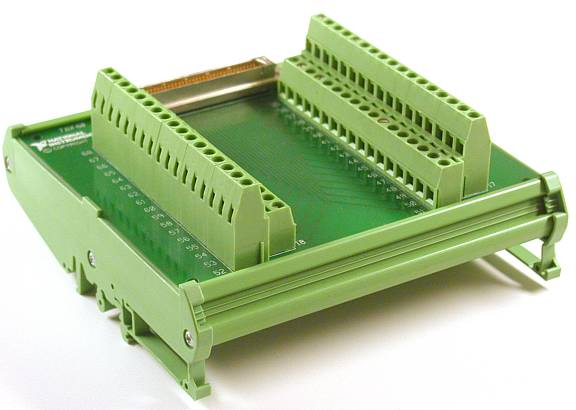
\includegraphics[scale=0.15]{FiguresP/NI-TBX-68}
\caption{Conector exterior para modulos de adquisicion PXI}
\label{fig:conexionPXI}
\end{figure}


En la tabla \ref{tab:signalsMaster} se muestra un listado de las señales digitales y analógicas del dispositivo maestro.

\newpage
\begin{sidewaystable}[htbp]
  \centering
  \caption{Listado de señales del robot maestro}
    \begin{tabular}{lllccccc}
    \toprule
    \multicolumn{8}{c}{\textbf{LISTADO DE SEÑALES ROBOT MAESTRO}} \\
    \hline
    \multicolumn{1}{c}{\multirow{2}{*}{\textbf{TAG}}} & \multicolumn{1}{c}{\multirow{2}{*}{\textbf{ORIGEN}}} & \multicolumn{1}{c}{\multirow{2}{*}{\textbf{DESCRIPCIÓN}}} & \multicolumn{1}{c}{\multirow{2}{*}{\textbf{TIPO SEÑAL}}} & \multicolumn{4}{c}{\textbf{SEÑAL}} \\  
  &  &  & & \textbf{DI} & \textbf{DO} & \textbf{AI} & \textbf{AO} \\
    \hline
   MAS-MSA & Maestro, Motor SA & Ref Motor, Salida Analógica, $\pm$10V & Comando &       &       &       & 1 \\
    MAS-MSE & Maestro, Motor SE & Ref Motor, Salida Analógica, $\pm$10V & Comando &       &       &       & 1 \\
    MAS-MEL & Maestro, Motor EL & Ref Motor, Salida Analógica, $\pm$10V & Comando &       &       &       & 1 \\
    MAS-MWY & Maestro, Motor WY & Ref Motor, Salida Analógica, $\pm$10V & Comando &       &       &       & 1 \\
    MAS-MWP & Maestro, Motor WP & Ref Motor, Salida Analógica, $\pm$10V & Comando &       &       &       & 1 \\
    MAS-RSA & Maestro, Motor SA & Ref Motor, Salida Analógica, $\pm$10V & Comando &       &       &       & 1 \\
    MAS-RSE & Maestro, Motor SE & Ref Motor, Salida Analógica, $\pm$10V & Comando &       &       &       & 1 \\
    MAS-REL & Maestro, Motor EL & Ref Motor, Salida Analógica, $\pm$10V & Comando &       &       &       & 1 \\
    MAS-RWY & Maestro, Motor WY & Ref Motor, Salida Analógica, $\pm$10V & Comando &       &       &       & 1 \\
    MAS-RWP & Maestro, Motor WP & Ref Motor, Salida Analógica, $\pm$10V & Comando &       &       &       & 1 \\
    MAS-PSA & Maestro, Potenciómetro SA & Potenciómetro Alimentado $\pm$10V & Medida &       &       & 1     &  \\
    MAS-PSE & Maestro, Potenciómetro SE & Potenciómetro Alimentado $\pm$10V & Medida &       &       & 1     &  \\
    MAS-PEL & Maestro, Potenciómetro EL & Potenciómetro Alimentado $\pm$10V & Medida &       &       & 1     &  \\
    MAS-PWY & Maestro, Potenciómetro WY & Potenciómetro Alimentado $\pm$10V & Medida &       &       & 1     &  \\
    MAS-PWP & Maestro, Potenciómetro WP & Potenciómetro Alimentado $\pm$10V & Medida &       &       & 1     &  \\
    MAS-PWR1 & Maestro, Potenciómetro WR1 & Potenciómetro Alimentado $\pm$10V & Medida &       &       & 1     &  \\
    MAS-PWR2 & Maestro, Potenciómetro WR2 & Potenciómetro Alimentado $\pm$10V & Medida &       &       & 1     &  \\
    MAS-PGRP & Maestro, Potenciómetro Gripper & Potenciómetro Alimentado $\pm$10V & Medida &       &       & 1     &  \\
    MAS-SHALT & Maestro, Pulsador Halt / Resume & Pulsador Sostenido & Pulsador & 1     &       &       &  \\
    MAS-SHYD & Maestro, Pulsador Hidráulica & Pulsador & Pulsador & 1     &       &       &  \\
    MAS-SWR & Maestro, Pulsador Wrist Mode & Pulsador & Pulsador & 1     &       &       &  \\
    MAS-SGRP & Maestro, Pulsador Gripper Lock & Pulsador & Pulsador & 1     &       &       &  \\
    MAS-LGRP & Maestro, Led Gripper Lock & Indicación, Led 5V, 15mA & Led   &       & 1     &       &  \\
    MAS-LWR & Maestro, Led Wrist Mode & Indicación, Led 5V, 15mA & Led   &       & 1     &       &  \\
    MAS-LHALT & Maestro, Led Halt / Resume & Indicación, Led 5V, 15mA & Led   &       & 1     &       &  \\
    MAS-LHYD & Maestro, Led Hidráulica & Indicación, Led 5V, 15mA & Led   &       & 1     &       &  \\
    \hline
    \multicolumn{4}{r}{\textbf{TOTAL}} & 4 & 4 & 8 & 10 \\
    \hline
    \end{tabular}%
  \label{tab:signalsMaster}%
\end{sidewaystable}%




\chapter{Reflexión de Fuerzas en el dispositivo maestro}
\begin{flushright}
\begin{minipage}{0,7\textwidth}

En este capitulo se presenta el diseño de una tarjeta de acondicionamiento de señal para convertir la corriente sinusoidal que fluye por los motores en una tensión de corriente continua para ser leído con mayor facilidad por el controlador de tiempo real. Posteriormente se presentan resultados experimentales realizados para estimar la relación entre la corriente consumida por los motores y la fuerza producida.

\end{minipage}
\end{flushright}



\newpage
En las últimas tres décadas la investigación en el control de fuerzas ha avanzado significativamente debido al gran interés de dotar a los sistemas robóticos de información y capacidades sensoriales. Los sensores de tacto, fuerza, distancia junto con la realimentación visual permiten la operación autónoma en entornos no estructurados.\\


Desde de las primeras investigaciones en el área de teleoperación el uso de la realimentación de fuerza fue concebido para ayudar al operador humano a manipular objetos en un entorno remoto con un manipulador esclavo. Recientemente se vienen utilizando sistemas robóticos cooperativos consistentes en dos o más manipuladores apoyándose entre s\'i para la realizaci\'on de las tareas.\\

El control de fuerza juega un papel muy importante en el comportamiento y versatilidad de los sistemas robóticos en entornos abiertos dotándoles de una respuesta inteligente en situaciones donde no hay visibilidad y permitiendo la interacción hombre-robot.\\



El control de la interacciones físicas entre el robot y su entorno es crucial para la ejecución de tareas donde el efector final del robot tiene que manipular objetos o realizar tareas en una superficie. Un ejemplo claro puede ser el pulido de una pieza recién pintada de un coche, donde la herramienta de pulido tiene siempre que estar en dirección normal a la superficie de trabajo. Otras aplicaciones donde se requiere el control de fuerza son operaciones de ensamblaje o mecanizado. Una clasificación completa de las tareas que requieren de un control de fuerza, incluyendo aplicaciones no industriales, es prácticamente imposible, debido a la gran cantidad de estas existentes, además de que no sería necesaria dicha clasificación para desarrollar una estrategia para controlar la interacción con el ambiente.\\


\section{Diseño de una tarjeta para medir la corriente en los motores del maestro }

La principal aportación de este trabajo fue la reflexión de fuerzas en el sistema maestro. Como se mencion\'o en el apartado de descripción de la plataforma de teleoperación, el sistema maestro es actuado por motores bifásicos de corriente alterna en cada uno de sus grados de libertad. Las señales de corriente alterna son generadas a través de una de las tarjetas de adquisición de datos del controlador de tiempo real (PXI) y posteriormente amplificadas en una etapa de potencia para suministrar la corriente necesaria a los motores.\\


Dado que el dispositivo maestro está equipado con motores bifásicos de CA que giran en un sentido o en otro dependiendo del desfase de las señales de entrada, el par ser\'a proporcional a la amplitud de la corriente.\\

\begin{figure}[ht!]
\centering
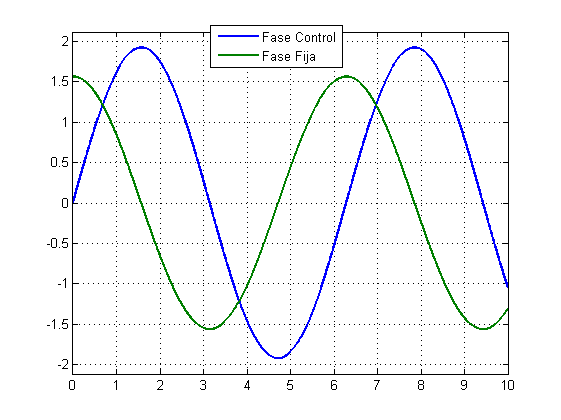
\includegraphics[scale=0.5]{FiguresP/entradaMotores}
\caption{Señales de entrada al motor}
\label{senalesmotor}
\end{figure}


El controlador del sistema esclavo toma mediciones de la fuerza aplicada en cada una de las articulaciones por medio de unos transductores de presión instalados en el interior de los actuadores hidráulicos. La información de los sensores de   presión se encuentra disponible en variables compartidas a través de Ethernet por medio del protocolo UDP.\\



Para reflejar y tener control sobre las fuerzas ejercidas en el dispositivo maestro la idea inicial fue medir la corriente directamente en cada una de las dos fases de cada motor. Un primer intento fue medir directamente el voltaje a través de los sensores de corriente (Sensores CS2.A03 ver figura \ref{fig:sensoresCorriente}) que entregan a su salida un voltaje proporcional a la corriente que circula por cada una de las dos fases. Para obtener una realimentación de la fuerza en cada uno de los cinco grados de libertad disponibles en el dispositivo fueron necesarios diez sensores de los antes mencionados.\\

\begin{figure}[!htb]
\centering
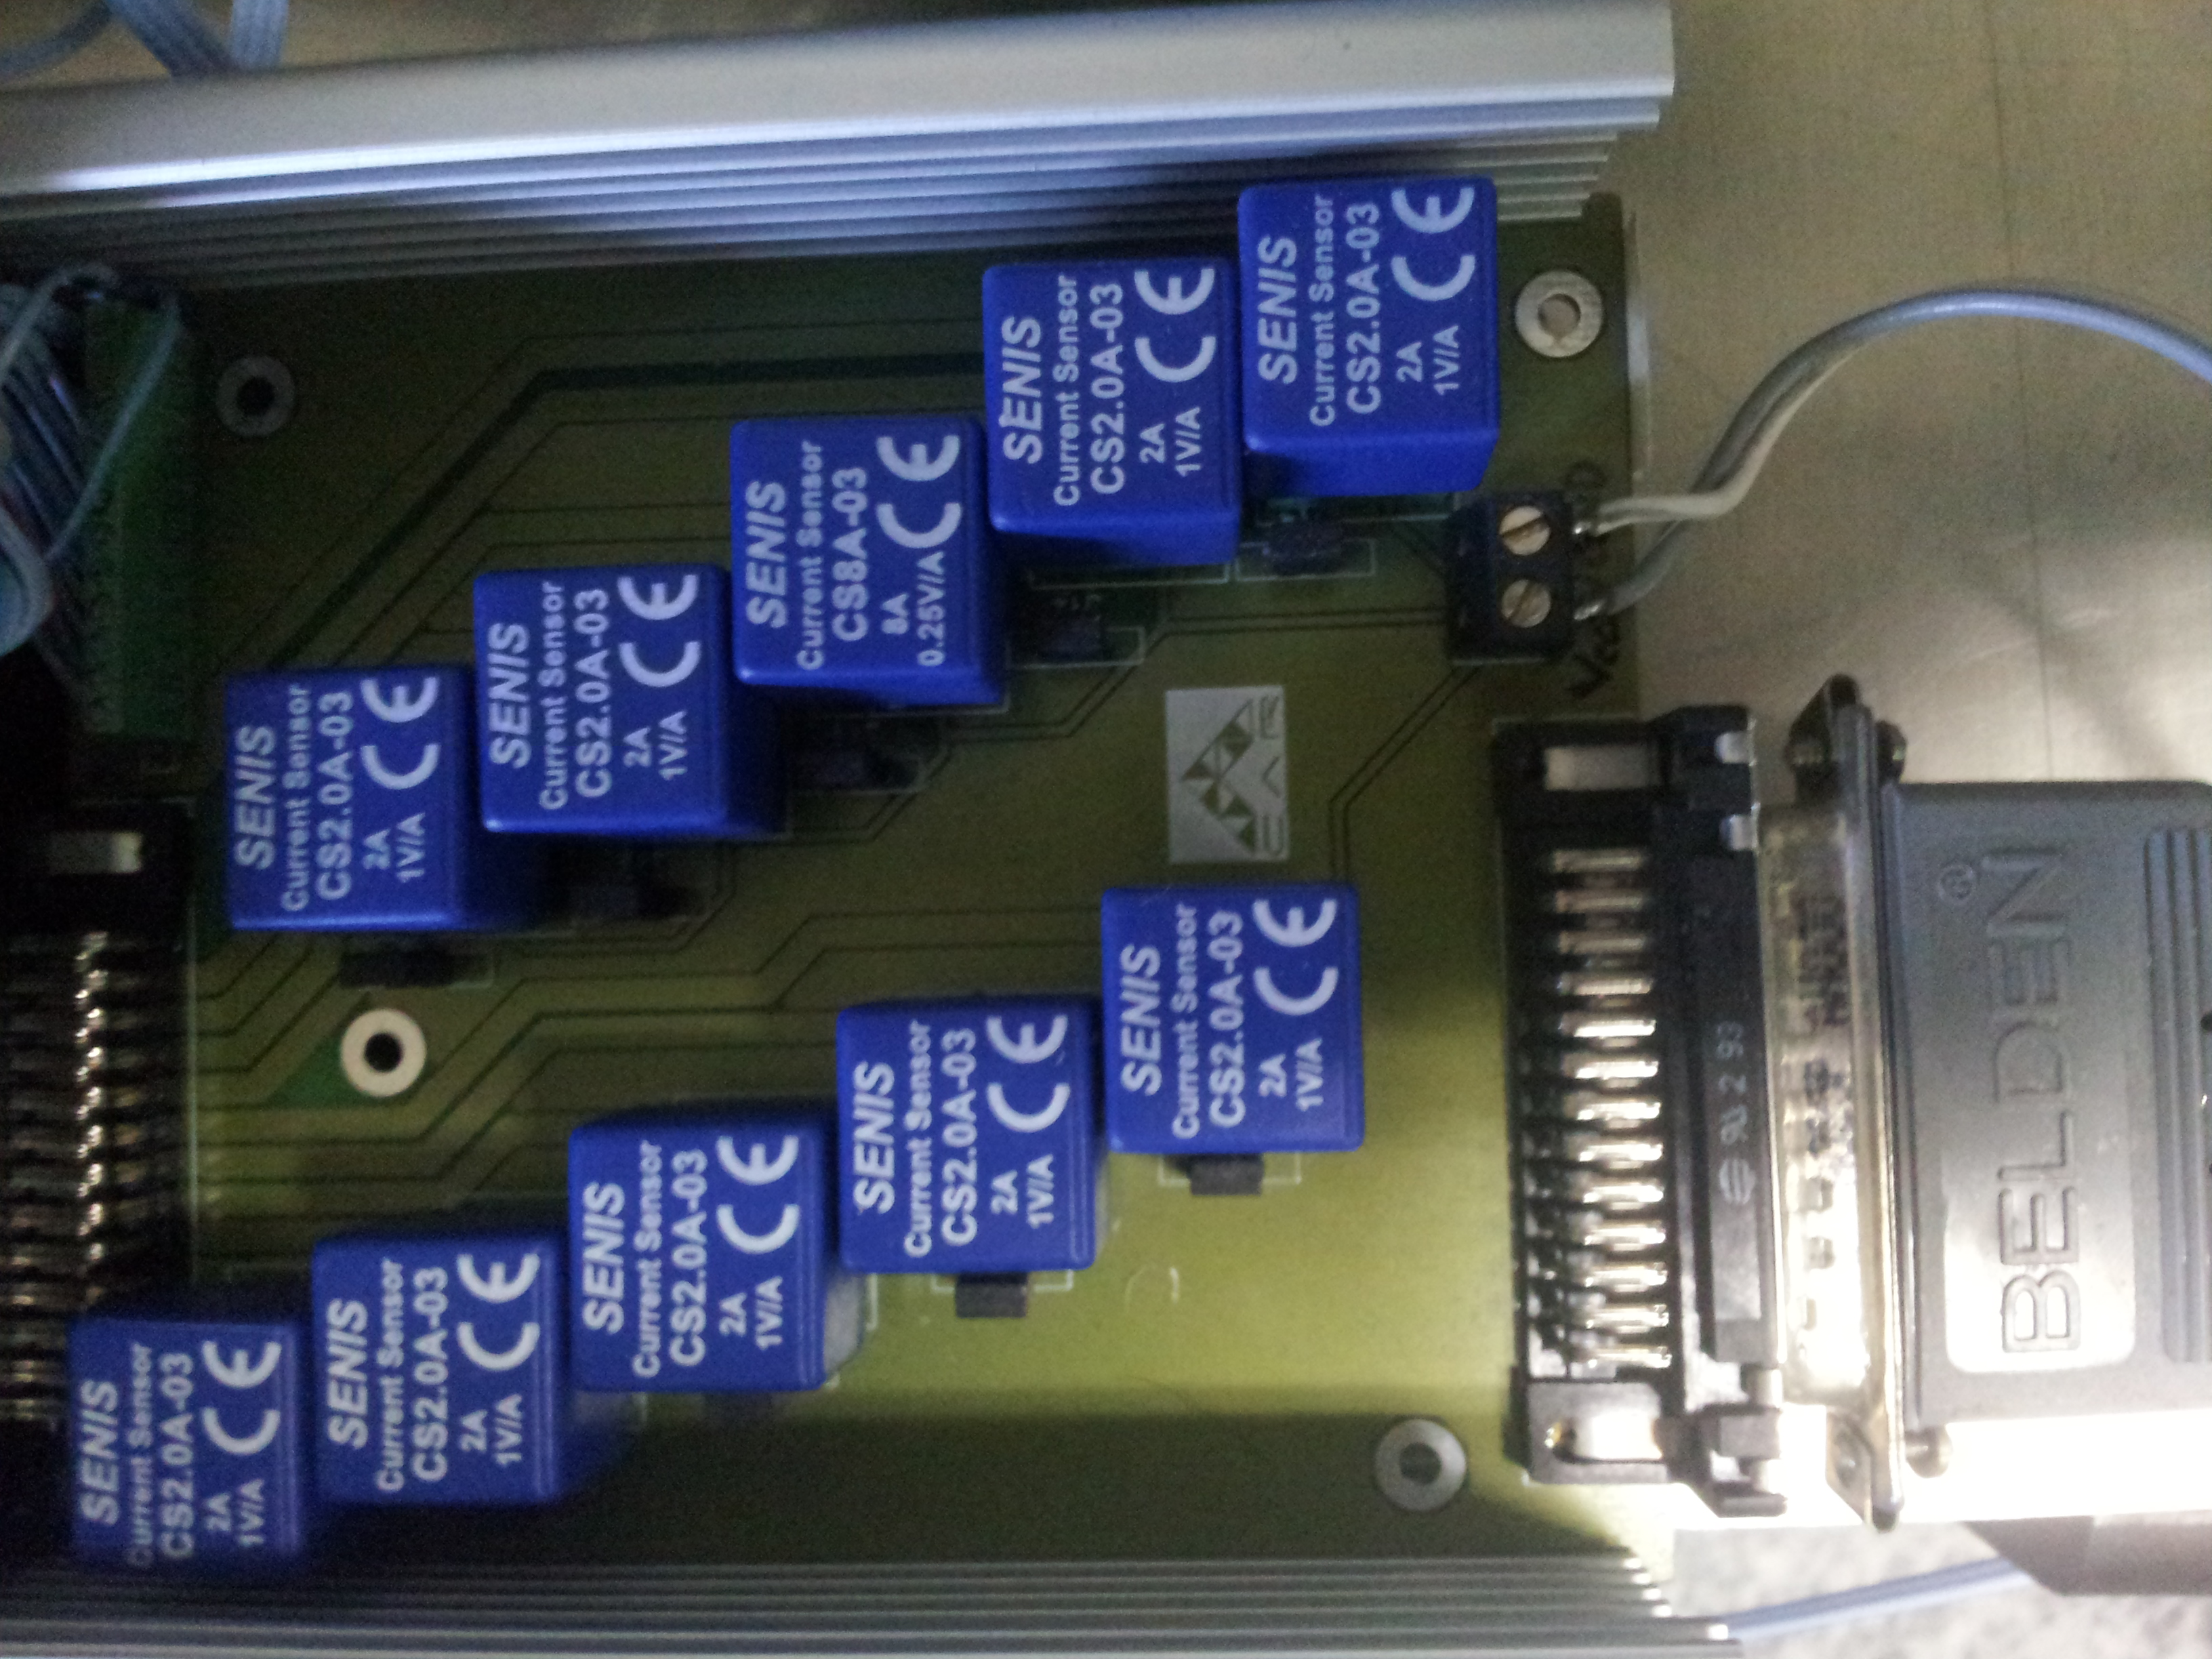
\includegraphics[scale=0.07]{FiguresP/CurrentSensors}
\caption{Tarjeta para leer la corriente a través de los motores del dispositivo maestro}
\label{fig:sensoresCorriente}
\end{figure}


El inconveniente de la propuesta inicial fue que había que tomar las lecturas de tensión en cada uno de los diez sensores. Después medir el desfase entre cada una con lo que ser\'ia necesario agregarle otro módulo de adquisición de entradas analógicas al controlador en tiempo real. Por otra parte había procesamiento excesivo por parte del controlador  para calcular el desfase de las señales de entrada y el valor eficaz vi\'endose afectadas partes críticas dedicadas a la comunicación y al control maestro-esclavo.\\


La solución propuesta fue diseñar un circuito de acondicionamiento capaz de convertir las diez señales sinusoidales provenientes de los sensores de corriente en cinco señales proporcionales al valor eficaz de la onda sinusoidal y con el signo dependiente del desfase de las señales de cada motor. \\

En el circuito de la figura \ref{fig:TarjetaCorriente} se puede observar la propuesta para el acondicionamiento de las señales de los sensores de corriente en los motores, el funcionamiento se describe a continuación:

\begin{description}
\item Un circuito integrado se encarga de calcular el valor eficaz de una de las formas de onda de los sensores de corriente, a la salida del circuito se entrega un valor de corriente directa proporcional al valor eficaz.

\item Por otro parte dos comparadores se encargan de detectar el cruce por cero de ambas señales sinusoidales, entregando un valor digital en cada cruce por cero

\item La salida de los detectores de cruce por cero es conectada a las entradas D y clk de un Flip-Flop tipo D con la finalidad de detectar el desfase de las señales, en caso de la fase de control este en adelanto con respecto a la fase fija la salida del Flip-Flop sera '1', en caso contrario sera '0'.

\item La señal de corriente directa proveniente del circuito que calcula el valor eficaz de una de las señales sinusoidales es multiplicada por un amplificador de instrumentación.

\item La salida Q del Flip-Flop tipo D se conecta al selector de un multiplexor analógico, que tiene como canales de entrada las salidas de ambos amplificadores de instrumentacion. Uno multiplica la señal de corriente continua por un valor positivo y el otro por un valor negativo. La salida del multiplexor es una señal de corriente continua cuya amplitud depende del valor eficaz de una de las ondas sinusoidales y cuyo signo depende del desfase entre ambas señales sinusoidales.


\end{description}



\begin{sidewaysfigure}
\centering
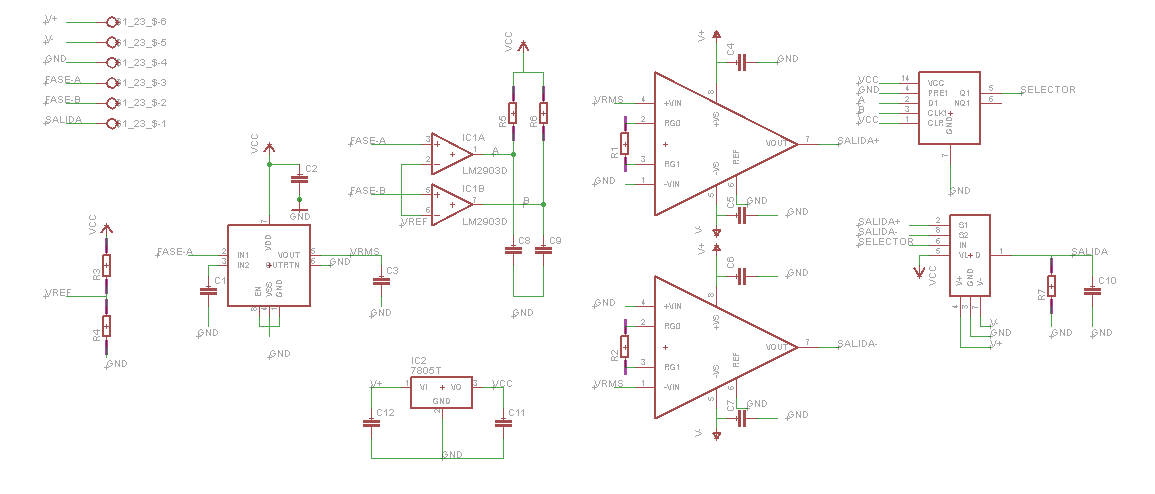
\includegraphics[scale=0.8]{FiguresP/EsquemaMotores}
\caption{Tarjeta para Mediciones de Corriente}
\label{fig:TarjetaCorriente}
\end{sidewaysfigure}



%
%Para realizar mediciones de la corriente que fluye a través de los motores se usaron sensores de corriente, los cuales producen un voltaje de salida pro proporcional a la corriente que fluye a través de ellos, con una sensibilidad de 1V/A, con lo cual en un principio se intento leer las señales de los sensores de corriente con uno de los módulos de adquisición de datos del controlador de tiempo real (ver figura \ref{fig:daq}), a través de un VI que detectara la diferencia de fase entre las dos señales de alimentación al motor(ver figura \ref{fig:señales}), y posteriormente medir el valor eficaz de una de las formas de onda. Al realizar pruebas se llego a la conclusión de que no era un método efectivo ya que era necesario emplear diez (10) entradas analógicas del modulo de adquisición de datos, es decir era necesario comprar otro modulo de entradas analógicas, y desperdiciar bastantes operaciones para encontrar un valor que fuese útil para la reflexión de fuerzas en el dispositivo maestro, con lo cual fue necesario diseñar un circuito electrónico para instrumentar dichas señales de control y pasar de tener  diez entradas analógicas a tener solo cinco, y en vez de tener formas de onda sinusoidales tener un voltaje de corriente directa proporcional (entre $\pm 4V$) a al valor eficaz de la forma de onda, con un signo positivo o negativo dependiendo del sentido de rotación del motor. 
% 









\begin{figure}
\centering
\includegraphics[scale=0.4]{FiguresP/CircuitoCorriente}
\caption{Tarjeta diseñada para el acondicionamiento de las señales de corriente en los motores}
\label{fig:TarjetaCorriente}
\end{figure}




%
%\begin{figure}
%\centering
%\includegraphics[scale=0.4]{FiguresP/Force}
%\caption{Tarjeta para Mediciones de Corriente}
%\label{fig:TarjetaCorriente}
%\end{figure}
%





\newpage
\section{Mediciones fuerza-corriente}
Para encontrar la relación entre la corriente que fluye por el motor y el par ejercido por el mismo se decidió montar un experimento y obtener mediciones (ver figura \ref{fig:montajeExperimento}). Para ello se utiliz\'o el sensor de fuerza ATI\textregistered SI-130 (ver figura \ref{fig:AtiForce2}), asignándose valores de corriente a través de lo motores a cada par y as\'i  encontrar una relación aproximada entre el par y la corriente consumida.


\begin{figure}[htb!]
\centering
\includegraphics[scale=0.7]{Figures/AtiConnection}
\caption{Sensor de fuerza y par en seis ejes ATI\textregistered con su módulo de conexiones}
\label{fig:AtiForce2}
\end{figure}

El sensor ATI \textregistered permite mediciones de par y fuerza en seis ejes gracias a su celda de carga multi-eje. El sensor cuenta con un sistema de adquisición de datos inteligente al que se puede acceder a través de una interfaz Ethernet/DeviceNet. Los rangos de medición así como las resoluciones máximas en cada uno de los ejes del sensor se muestran en la tabla \ref{tab:ati}\\

\begin{table}[htb!]
\begin{flushleft}
\begin{tabular}{ c c c c c c c c  }
& & Rango de Sensibilidad   &  &  &  &   Resolución  &\\
\hline
Calibración &	Fx,Fy &	Fz     &	Tx,Ty &	Tz	  & Fx,Fy  &	Fz	    &  Tx,Ty,Tz \\
\hline
SI-130-10	& 130 N   &	400 N  & 10 Nm  &	10 Nm  &	1/40 N &	1/20 N 	& 1/800 Nm  \\
\hline
\end{tabular}
\end{flushleft}
\caption{Calibración métrica  (SI)  del Sensor ATI}
\label{tab:ati}
\end{table}


Para realizar la adquisición de datos fue necesario crear una interfaz visual (del ingl\'es \textit{ Interfase} VI) en Labview para capturar de manera paralela las lecturas de los sensores de corriente y la información acerca de la fuerza en un eje del sensor ATI. El VI diseñado est\'a encargado de establecer una conexión ethernet entre ambos dispositivos y capturando los datos en un archivo \textbf{.mat} de Matlab, para posteriormente hacer el tratamiento de los mismo y hacer un ajuste de curva.\\


\begin{figure}[htb!]
%\subfigure[Montaje para la medición de fuerza del sensor $ATI^{\textregistered}$]{\includegraphics[scale=0.12]{FiguresP/setupTorque1}\label{fig:current}}

\includegraphics[scale=0.12]{FiguresP/setupTorque2}\label{fig:force}
\caption{Montaje del experimento para la medición de fuerza de la fuerza ejercida por el maestro usando el sensor $ATI^{\textregistered}$}
\label{fig:montajeExperimento}
\end{figure}

%\section{Mediciones de Par ejercido por los Motores con el sensor ATI\textregistered}

%\begin{figure}[htb!]
%\centering
%\includegraphics[scale=0.5]{Figures/AtiSensor}
%\caption{Sensor de Fuerza y Torque en seis ejes ATI\textregistered}
%\label{fig:AtiForce}
%\end{figure}


%\newpage
%\begin{figure}
%\subfigure[Corriente Medida a traves las tarjetas diseñadas]{\includegraphics[scale=0.4]{FiguresP/Current}\label{fig:current}}
%\subfigure[Medicion de fuerza del sensor $ATI^{\textregistered}$]{\includegraphics[scale=0.4]{FiguresP/Force}\label{fig:force}}
%\caption{Mediciones obtenidas del experimento para determinar la relacion entre la corriente y el par}
%\end{figure}


\newpage
\section{Modelo del motor Corriente VS Fuerza}
Con los datos obtenidos a partir de las mediciones del experimento se obtuvo un ajuste de curva usando Matlab. Los datos obtenidos de los sensores pueden verse en la figura \ref{fig:MedicionesFuerzaCorriente}. El eje de las \textbf{X} es el tiempo transcurrido durante el experimento mientras que el eje de las \textbf{Y} corresponde a los valores obtenidos de ambos sensores. Para el caso del sensor de fuerza la magnitud se dividió entre diez para una mayor comodidad a la hora de ver la gráfica.




\begin{figure}[htb!]
\centering
\includegraphics[scale=0.4]{FiguresP/ForceCurrent}
\caption{Tarjeta para mediciones de corriente}
\label{fig:MedicionesFuerzaCorriente}
\end{figure}


A partir de una aproximación por mínimos cuadrados se encontró la ecuación que relaciona la fuerza de los motores con la corriente:

\subsection*{Modelo lineal}

\begin{equation}
f(x) = p_1x + p_2
\end{equation}
     
coeficientes (con unos límites de confianza del 95\% ):
		$$       p_1 =       17.93  (17.51, 18.34)$$       
       $$       p_2 =      -15.65  (-16.73, -14.58) $$
  Calidad de la aproximación:\\
  SSE: 4.646e+004\\
  R-cuadrada: 0.8794\\
  R-cuadrada ajustada: 0.8792\\  
  RMSE: 6.903


\subsection*{Modelo cuadrático}
\begin{equation}
     f(x) = p_1 x^2 + p_2x + p_3
\end{equation}

Coeficientes (con unos límites de confianza del 95\% ):
$$     p_1 =      0.8509  (0.3606, 1.341)$$
$$       p_2 =       13.92  (11.57, 16.26)$$       
$$       p_3 =      -11.85  (-14.29, -9.41)$$

  Calidad de la aproximación:\\
  SSE: 4.592e+004\\
  R-cuadrada: 0.8808\\
  R-cuadrada ajustada: 0.8805\\
  RMSE: 6.866





\begin{figure}[htb!]
\centering
\includegraphics[scale=0.5]{FiguresP/ModeloFC}
\caption{Modelos hecho por aproximación de mínimos cuadrados}
\label{fig:curveFitting}
\end{figure}

Analizando la figura \ref{fig:curveFitting} se concluye que no existe mucha diferencia entre el modelo lineal y el modelo cuadrático, con lo cual es preferible usar el modelo lineal para simplificar las operaciones.

%\section{Caracterización del sistema Maestro}
%Posterior al diseño del circuito electrónico para la medición de corriente en los motores de cada una de las articulaciones del sistema maestro.


\section{Bucle de Control en Fuerza}

Para la reflexión de fuerzas en el maestro del manipulador grips se propone el uso de un regulador proporcional integral con las siguientes ganancias:

\begin{equation}
K=3.00 \qquad    T_i=0.001s \qquad   dt=0.001s
\end{equation}



\begin{figure}[htb!]
\centering
\caption{Esquema de control en corriente de los motores del dispositivo maestro}
\includegraphics[scale=0.5]{FiguresP/Controller}
\end{figure}






\graphicspath{{./FiguresA/}}
\chapter{Evaluación de Diferentes Arquitecturas de Control para Teleoperación}
\label{ch:arquitecturas}
El objetivo de este capítulo es comprobar de manera experimental los principales algoritmos de control bilateral así como sus ventajas e inconvenientes.

\begin{figure}[htbp]
\centering
	\includegraphics[scale=0.2]{setup.jpg}
	\caption{Fotografía de la plataforma experimental}
  	\label{fig:setup}
\end{figure}
Este trabajo se ha desarrollado en la plataforma experimental mostrada en la figura \ref{fig:setup}, donde la implementación de los algoritmos se realiza utilizando el entorno de desarrollo LABVIEW.\\
Los elementos principales de la plataforma experimental son:
\begin{itemize}
\item 2 x Motor Maxon, serie RE 25, reductor planetario GP 26 B (1:104), encoder MR.
\item 1 x Controlador compact RIO 9022 dotado de una FPGA.
\item 2 x NI 9505 Módulo de Drive Servo de DC de Escobillas con Puente H Completo.
\item 2 x NI 9205 Módulo de Entrada Analógica de 32 Canales.
\end{itemize}

El modelo de ambos motores, maestro y esclavo, que se ha utilizado es el siguiente:
\begin{eqnarray}
\dfrac{\theta(s)}{I(s)} &=& \dfrac{A}{(J s^2+B s)} = \dfrac{4.5552}{0.0118s^2 + 2.8607s} \\[0.5cm]
F \cdot 0.16 &=& R_T K_\tau I \nonumber
\label{eq:model}
\end{eqnarray}
Donde,
\begin{itemize}
\item $F$ es la fuerza aplicada al dispositivo.
\item $R_T$ es el factor de reducción de los motores e igual a 104.
\item $K_\tau$ es la constante de par de los motores e igual a $43.8\cdot 10^{-3} \frac{Nm}{A}$.
\item $I$ es la intensidad que fluye por los motores. Máximo 0.7 A.
\end{itemize}
\begin{figure}[htbp]
\centering
	\includegraphics[scale=0.5]{cascada}
	\caption{Diagrama de bloques del control implementado en cada motor} % labelInTOC
  	\label{fig:cascada} %% label for entire figure
\end{figure}
Otro aspecto a tener en cuenta es el tipo de control implementando en cada motor ya que con el objetivo de protegerlos se utiliza un esquema en cascada como se muestra en la figura \ref{fig:cascada}. Para los propósitos de este trabajo solo se ha considerado el regulador $R_1(s)$ ya que el lazo interno responde más rápido (hasta 10 veces más rápido) y se puede considerar únicamente su valor en régimen permanente, la unidad, ya que $R_2(s)$ es un regulador PI (error nulo en régimen permanente).
\begin{figure}[htbp]
\centering
	\includegraphics[scale=0.6]{fixedPointPID}
	\caption{Fixed Point PID VI} 
  	\label{fig:fixedPID}
\end{figure}
Con respecto a $R_1(s)$ cabe mencionar que se ha utilizado el VI mostrado en la figura \ref{fig:fixedPID}. Este PID permite gran flexibilidad ya que se pueden probar reguladores clásicos así como versiones mejoradas en las que se considera la velocidad o aceleración del motor. En la figura \ref{fig:pidloop} se muestra de manera gráfica como se relacionan los diferentes parámetros y ganancias con las que cuenta el VI en cuestión.
\begin{figure}[htbp]
\centering
	\includegraphics[scale=0.5]{pidloop} 
	\caption{NI SoftMotion Control Loop} 
  	\label{fig:pidloop} 
\end{figure}

\section{Control Posición - Posición}
\label{sec:pos-pos}
En esta sección se realiza en primer lugar un análisis teórico de la estabilidad y de la percepción por parte del operador en este tipo de algoritmo en sus casos extremos:
\begin{itemize}
\item Espacio libre: La impedancia del entorno es nula ($K_e = 0$), el esclavo se mueve libremente, y la única fuerza externa que actúa sobre el sistema es la del operador sobre el maestro.
\item Contacto con un objeto rígido: El esclavo esta en contacto con un entorno rígido ideal ($K_e = \infty$).
\end{itemize}
Posteriormente se presentaran algunos resultados obtenidos en la plataforma experimental.
\begin{figure}[htbp]
\centering
	\includegraphics[scale=0.5]{pos-pos}
	\caption{Arquitectura de control Posición - Posición} % labelInTOC
  	\label{fig:pos-pos} %% label for entire figure
\end{figure}

En la figura \ref{fig:pos-pos} se muestra la arquitectura en cuestión. Con el fin de analizar los casos extremos y como serán percibidos por el operador es necesario simplificar este diagrama de bloques reemplazando el valor de $K_e$.
\begin{figure}[htbp]
\centering
	\begin{subfigure}[h]
		\centering
		\includegraphics[scale=0.5]{pos-pos-operator}
		\caption{Esquema visto desde el maestro}
	\end{subfigure}
	\begin{subfigure}[h]
		\centering
		\includegraphics[height=4cm]{pos-pos-kvalues}
		\caption{Casos extremos}
    \end{subfigure}
	\caption{Diagrama de bloques para los casos extremos del control Posición - Posición}
  	\label{fig:pos-pos-casos}
\end{figure}

En la figura \ref{fig:pos-pos-casos} se muestran los diagramas simplificados así como las funciones de transferencia resultantes en los casos extremos.
\\
No es necesario entrar en el detalle de los modelos del maestro y esclavo para intuir la percepción por parte del operador:
\begin{itemize}
\item $K_e = 0$: $H(s)$ esta dada por $\frac{K_{pm}}{1+K_{ps}S(s)}$ con lo cual el operador percibirá cierta fuerza a pesar de que ninguna fuerza se esta ejerciendo sobre el esclavo.
\item $K_e = \infty$: $H(s)$ esta dada por $K_{pm}$ con lo cual la máxima impedancia que percibirá el operador esta determinada por el regulador (P, PD, etc.) del maestro ($K_{pm}$).
\end{itemize}

En lo que concierne a la estabilidad de este sistema se puede analizar también en los casos extremos. En aras de la sencillez se considerará el caso en que los dos reguladores $K_{pm}$ y $K_{ps}$ son proporcionales.
Retomando el modelo del sistema de la ecuación \eqref{eq:model} y aplicando la relación para expresarlo en función de la fuerza tenemos:
\begin{equation}
G(s) = \dfrac{\theta(s)}{F(s)} = \dfrac{4.5552}{0.0118s^2 + 2.8607s}\cdot \dfrac{0.16}{R_tK_t} = \dfrac{0.16}{0.0118 s^2 + 2.861 s}
\end{equation}
\begin{itemize}
\item $K_e = 0$:
\begin{equation}
G_r(s) = \dfrac{M(s)}{1 + M(s)\dfrac{K_{pm}}{1 + K_{ps}S(s)}} = \dfrac{0.16}{0.0118 s^2 + 2.861 s + 0.16(K_{pm} + K_{ps})}
\end{equation}
\begin{table}[htbp]
  \centering
  \caption{Tabla del criterio de Routh-Hurwitz para $K_e = 0$ (Posición - Posición)}
    \begin{tabular}{ccc}
    \toprule
    $s_2$	& $0.0118$		& $0.16(K_{pm} + K_{ps})$ \\
    $s_1$	& $2.861$		& 	\\
 	$s_0$	& $0.16(K_{pm} + K_{ps})$		& 	\\
    \bottomrule
    \end{tabular}
  \label{tab:routh-pos-pos0}
\end{table}
Donde $G_r(s)$ es la función de transferencia en lazo cerrado. Aplicando el criterio de estabilidad de Routh-Hurwitz (Tabla \ref{tab:routh-pos-pos0}), el cual establece que para que el sistema sea estable no deben presentarse cambios de signo en la primer columna, se comprueba que el sistema es estable para todos los valores \textbf{positivos} de $K_{pm}$ y $K_{ps}$.

\item $K_e = \infty$:
\begin{equation}
G_r(s) = \dfrac{M(s)}{1 + M(s)\dfrac{K_{pm}}{1 + K_{ps}S(s)}} = \dfrac{0.16}{0.0118 s^2 + 2.861 s + 0.16K_{pm}}
\end{equation}
\begin{table}[htbp]
  \centering
    \caption{Tabla del criterio de Routh-Hurwitz para $K_e = \infty$ (Posición - Posición)}
    \begin{tabular}{ccc}
    \toprule
    $s_2$	& $0.0118$		& $0.16K_{pm}$ \\
    $s_1$	& $2.861$		& 	\\
 	$s_0$	& $0.16K_{pm}$		& 	\\
    \bottomrule
    \end{tabular}%
  \label{tab:routh-pos-pos1}%
\end{table}%
Aplicando el criterio de estabilidad de Routh-Hurwitz (Tabla \ref{tab:routh-pos-pos1}) se comprueba que el sistema es estable para todos los valores \textbf{positivos} de $K_{pm}$.
\end{itemize}

\subsection{Simulación del Sistema}
\label{sub:pos-pos-sim}
Con el fin de comprobar el funcionamiento del sistema se ha diseñado un regulador PD para controlar tanto al maestro ($K_{pm}$) como el esclavo ($K_{ps}$). Se podría pensar que el regulador PID sería una mejor opción, pero la acción integral no es recomendable por varias razones, entre ellas las siguientes:
\begin{itemize}
\item La intención no es sólo que el regulador fuerce al sistema a ir a la posición deseada, sino que también refleje las fuerzas de la forma más clara y real posible. Con este fin, no tiene ningún sentido que ante un error de posición constante, la salida de nuestro controlador aumente y con ello aumenten las fuerzas que se representan en el maestro, tiene más sentido que estas sean constantes pues las fuerzas a las que esta sometido el esclavo en este caso particular son constantes.
\item Al ser un proceso con gran cantidad de no linealidades (p. ej. los choques del esclavo contra el entorno) habría que incluir un Wind-Up, ya que si no se controla la acción integral se perjudicaría mucho el sistema.
\end{itemize}
Para el diseño del regulador se ha considerado cada motor de manera independiente y dado que son idénticos se tiene:
\begin{equation}
M(s) = S(s) = \dfrac{\theta(s)}{F(s)} = \dfrac{0.16}{0.0118 s^2 + 2.861 s}
\label{eq:force-motor-model}
\end{equation}
Teniendo en cuenta que el tiempo de muestreo es $T = 1$ ms, la ecuación \eqref{eq:force-motor-model} se discretiza como:
\begin{equation}
M(z) = S(z) = \dfrac{\theta(z)}{F(z)} = \dfrac{6.2634\cdot 10^{-6}(z+0.9224)}{(z-1)(z-0.7847)}
\end{equation}
Utilizando la \mcode{rtool} de MATLAB y definiendo las siguientes especificaciones:
\begin{equation*}
M_p \leq 10\% \quad t_s \leq 50 \mbox{ms} \quad e_p = 0
\end{equation*}
Se ha diseñado un regulador PD que permitirá controlar en posición cada motor. En la figura \ref{fig:pos-pos-reg} se muestra el lugar de las raíces resultante así como la respuesta del sistema en lazo cerrado ante entrada escalón unitario.
\begin{figure}[htbp]
\centering
	\begin{subfigure}[h]
		\centering
		\includegraphics[height=5.25cm]{pos-pos-rlocus}
		\caption{Lugar de las raíces}
	\end{subfigure}
	\begin{subfigure}[h]
		\centering
		\includegraphics[height=5.25cm]{pos-pos-step}
		\caption{Respuesta ante entrada escalón unitario}
    \end{subfigure}
	\caption{Respuesta del PD diseñado para control en posición de cada motor}
  	\label{fig:pos-pos-reg}
\end{figure}

La función de transferencia de dicho regulador es:
\begin{equation}
R(z) = \dfrac{K(z-c_d)}{z} = \dfrac{1100(z-0.2)}{z}
\label{eq:regulador}
\end{equation}
Se ha comprobado el funcionamiento del sistema en su conjunto en el modelo de SIMULINK que se muestra en la figura \ref{fig:pos-pos-esq}.
\begin{figure}[htbp]
\centering
	\includegraphics[width=10cm]{pos-pos-esq}
	\caption{Esquema de control Posición - Posición en Simulink}
  	\label{fig:pos-pos-esq}
\end{figure}
En la figura \ref{fig:pos-pos-sim} se muestran los resultados obtenidos para los casos extremos que se han planteado.
\begin{figure}[htbp]
\centering
	\begin{subfigure}[h]
		\centering
		\includegraphics[height=5.25cm]{pos-pos-libre}
		\caption{$K_e = 0$, entrada sinusoidal}
	\end{subfigure}
	\begin{subfigure}[h]
		\centering
		\includegraphics[height=5.25cm]{pos-pos-env}
		\caption{Respuesta ante entrada escalón unitario}
    \end{subfigure}
	\caption{Simulación del control Posición - Posición}
  	\label{fig:pos-pos-sim}
\end{figure}

\subsection{Experimentos}
\label{sub:pos-pos-exp}
\begin{figure}[htbp]
\centering
	\begin{subfigure}[h]
		\centering
		\includegraphics[height=5.25cm]{pos-pos-exp-libre}
		\caption{Movimiento libre}
		\label{fig:pos-pos-exp-libre}
	\end{subfigure}
	\hspace{0.1cm}
	\begin{subfigure}[h]
		\centering
		\includegraphics[height=5.25cm]{pos-pos-exp-env}
		\caption{Colisión contra objeto rígido (t $\simeq$ 4-8 s.)}
		\label{fig:pos-pos-exp-env}
    \end{subfigure}
	\caption{Resultados experimentales del control Posición - Posición}
  	\label{fig:pos-pos-exp}
\end{figure}

Con el regulador diseñado se han realizado experimentos para comprobar el funcionamiento del sistema.
\begin{itemize}
\item Movimiento libre: En la figura \ref{fig:pos-pos-exp-libre} se muestra como en el movimiento libre el maestro y el esclavo tienen la misma posición con error prácticamente nulo. Respecto a la fuerza percibida por el operador se aprecia que a pesar de estar en movimiento libre es necesario realizar hasta 3N para modificar la posición del sistema.
\item Colisión: En la figura \ref{fig:pos-pos-exp-env} se puede observar como durante el periodo de tiempo comprendido entre 4 y 8 segundos hay un error significativo en la posición. Además por la lectura de fuerza se puede ver que el pico de fuerza realizado por el operador alcanza los -19 Newtons.
\end{itemize}

\section{Control Fuerza - Posición}
\label{sec:force-position}
En esta sección se realiza en primer lugar un análisis teórico de la estabilidad y de la percepción por parte del operador en este tipo de algoritmo en sus casos extremos:
\begin{itemize}
\item Espacio libre: La impedancia del entorno es nula ($K_e = 0$), el esclavo se mueve libremente, y la única fuerza externa que actúa sobre el sistema es la del operador sobre el maestro.
\item Contacto con un objeto rígido: El esclavo esta en contacto con un entorno rígido ideal ($K_e = \infty$).
\end{itemize}
Posteriormente se presentaran algunos resultados obtenidos en la plataforma experimental.
\begin{figure}[htbp]
\centering
	\includegraphics[height=8cm]{force-pos}
	\caption{Arquitectura de control Fuerza - Posición}
  	\label{fig:force-pos} 
\end{figure}
En la figura \ref{fig:force-pos} se muestra la arquitectura en cuestión. Con el fin de analizar los casos extremos y como serán percibidos por el operador es necesario simplificar este diagrama de bloques reemplazando el valor de $K_e$.
\begin{figure}[htbp]
\centering
	\begin{subfigure}[h]
		\centering
		\includegraphics[height=4cm]{force-pos-operator}
		\caption{Esquema visto desde el maestro}
	\end{subfigure}
	\begin{subfigure}[h]
		\centering
		\includegraphics[height=4cm]{force-pos-kvalues}
		\caption{Casos extremos}
    \end{subfigure}
	\caption{Diagrama de bloques para los casos extremos del control Fuerza - Posición}
  	\label{fig:force-pos-casos}
\end{figure}

En la figura \ref{fig:force-pos-casos} se muestran los diagramas simplificados así como las funciones de transferencia resultantes en los casos extremos.
\\
No es necesario entrar en el detalle de los modelos del maestro y esclavo para intuir la percepción por parte del operador:
\begin{itemize}
\item $K_e = 0$: No hay $H(s)$. Con lo cual el operador no percibirá ninguna fuerza por la interacción con el entorno sino solamente las inherentes a la masa e inercia del maestro (dinámica del maestro $M(s)$).
\item $K_e = \infty$: $H(s)$ esta dada por $K_{f}K_{ps}$ con lo cual la máxima impedancia que percibirá el operador esta determinada por el regulador (P, PD, etc.) del esclavo ($K_{ps}$) y el factor con el que se refleja la fuerza $K_{f}$.
\end{itemize}

En lo que concierne a la estabilidad de este sistema se puede analizar también en los casos extremos. En aras de la sencillez se considerará el caso en que el regulador $K_{ps}$ y el factor $K_{f}$ son proporcionales.
Retomando el modelo del sistema de la ecuación \eqref{eq:model} y aplicando la relación para expresarlo en función de la fuerza tenemos:
\begin{equation}
G(s) = \dfrac{\theta(s)}{F(s)} = \dfrac{4.5552}{0.0118s^2 + 2.8607s}\cdot \dfrac{0.16}{R_tK_t} = \dfrac{0.16}{0.0118 s^2 + 2.861 s}
\end{equation}
\begin{itemize}
\item $K_e = 0$: Tenemos un lazo abierto de un sistema que es estable, y por lo tanto tendremos una salida acotada.

\item $K_e = \infty$: La ecuación en del sistema realimentado será:
\begin{equation}
G_r(s) = \dfrac{M(s)}{1 - M(s)K_{ps}K_f} = \dfrac{0.16}{0.0118 s^2 + 2.861 s + 0.16(K_f+K_{ps})}
\end{equation}
\begin{table}[htbp]
  \caption{Tabla del criterio de Routh-Hurwitz para $K_e = \infty$ (Fuerza - Posición)}
  \centering
    \begin{tabular}{ccc}
    \toprule
    $s_2$	& $0.0118$		& $0.16(K_f+K_{ps})$ \\
    $s_1$	& $2.861$		& 	\\
 	$s_0$	& $0.16(K_f+K_{ps})$		& 	\\
    \bottomrule
    \end{tabular}
  \label{tab:force-pos-routh}
\end{table}
Aplicando el criterio de estabilidad de Routh-Hurwitz (Tabla \ref{tab:force-pos-routh}) se comprueba que el sistema es estable para todos los valores \textbf{positivos} de $K_{f}$ y $K_{ps}$.
\end{itemize}

\subsection{Simulación del Sistema}
\label{sub:force-pos-sim}
En esta sección se utilizará el regulador obtenido en el numeral \ref{sub:pos-pos-sim}, correspondiente a la ecuación \eqref{eq:regulador}.
\\
Se ha comprobado el funcionamiento del sistema en su conjunto en el modelo de SIMULINK que se muestra en la figura \ref{fig:force-pos-esq}.
\begin{figure}[htbp]
\centering
	\includegraphics[width=10cm]{force-pos-esq}
	\caption{Esquema de control Fuerza - Posición en Simulink}
  	\label{fig:force-pos-esq}
\end{figure}
En la figura \ref{fig:force-pos-sim} se muestran los resultados obtenidos para los casos extremos que se han planteado.
\begin{figure}[htbp]
\centering
	\begin{subfigure}[h]
		\centering
		\includegraphics[height=5.25cm]{force-pos-libre}
		\caption{$K_e = 0$, entrada sinusoidal}
	\end{subfigure}
	\begin{subfigure}[h]
		\centering
		\includegraphics[height=5.25cm]{force-pos-env}
		\caption{$K_e = 100$, entrada escalón unitario}
	\end{subfigure}
	\caption{Simulación del control Fuerza - Posición}
  	\label{fig:force-pos-sim}
\end{figure}

\subsection{Experimentos}
\label{sub:force-pos-exp}
\begin{figure}[htbp]
\centering
	\begin{subfigure}[h]
		\centering
		\includegraphics[height=5.25cm]{force-pos-exp-libre}
		\caption{Movimiento libre}
		\label{fig:force-pos-exp-libre}
	\end{subfigure}
	\begin{subfigure}[h]
		\centering
		\includegraphics[height=5.25cm]{force-pos-exp-env}
		\caption{Colisión contra objeto rígido (t $\simeq$ 4-7 s. )}
		\label{fig:force-pos-exp-env}
	\end{subfigure}
	\caption{Resultados experimentales del control Fuerza - Posición}
  	\label{fig:force-pos-exp}
\end{figure}

Con el regulador diseñado se han realizado experimentos para comprobar el funcionamiento del sistema.
\begin{itemize}
\item Movimiento libre: En la figura \ref{fig:force-pos-exp-libre} se muestra como en el movimiento libre el maestro y el esclavo tienen la misma posición con error prácticamente nulo. Respecto a la fuerza percibida por el operador se aprecia que a pesar de estar en movimiento libre es necesario realizar hasta 3N para modificar la posición del sistema, aunque si se compara con el caso del control Posición - Posición (Numeral \ref{sub:pos-pos-exp}) el rango de posiciones alcanzadas es mayor.
\item Colisión: En la figura \ref{fig:force-pos-exp-env} se puede observar como durante el periodo de tiempo comprendido entre 4 y 7 segundos hay un error significativo en la posición. Además por la lectura de fuerza se puede ver que el pico de fuerza realizado por el operador alcanza los 17N y por otro lado la fuerza realizada por el esclavo en el entorno no supera los 8N.
\end{itemize}

\section{Arquitectura de Cuatro Canales}
\label{sec:4canales}
\begin{figure}[htbp]
\centering
	\includegraphics[width=\textwidth]{four}
	\caption{Arquitectura de control de 4 Canales} % labelInTOC
  	\label{fig:four} %% label for entire figure
\end{figure}
En esta sección se presentan los resultados obtenidos al utilizar la arquitectura de cuatro canales (figura \ref{fig:four}) en la plataforma experimental de la figura \ref{fig:setup}.
\begin{figure}[htbp]
\centering
	\begin{subfigure}[h]
		\centering
		\includegraphics[height=5.25cm]{four-exp-libre}
		\caption{Movimiento  libre}
		\label{fig:four-exp-libre}
	\end{subfigure}
	\begin{subfigure}[h]
		\centering
		\includegraphics[height=5.25cm]{four-exp-env}
		\caption{Colisiones en $t\simeq 0-1.5$ s. y $t\simeq 5-10$ s.}
		\label{fig:four-exp-env}
	\end{subfigure}		
	\caption{Resultados experimentales de la Arquitectura de Cuatro Canales}
  	\label{fig:four-exp}
\end{figure}

Se han realizado experimentos en los casos extremos que se han mencionado anteriormente:
\begin{itemize}
\item Movimiento libre ($Z_e = 0$): En la figura \ref{fig:four-exp-libre} se muestra como en el movimiento libre el maestro y el esclavo tienen la misma posición con error prácticamente nulo. Respecto a la fuerza que el operador debe realizar para modificar la posición del sistema, se aprecia que tan solo es necesario aplicar fuerza cuando se cambia la dirección del movimiento y aún así la fuerza requerida es del orden de 1N. Si se comparan estos resultados con aquellos obtenidos con Posición - Posición (Fig. \ref{fig:pos-pos-exp-libre}) y con Fuerza - Posición (Fig. \ref{fig:force-pos-exp-libre}) salta a la vista que la arquitectura de cuatro canales permite una mejor percepción del entorno.

\item Colisión ($Z_e = \infty$): En la figura \ref{fig:four-exp-env} se muestran los resultados de dos colisiones con un entorno rígido. En $t\simeq 0-1.5$ seg. se puede advertir que la colisión se ha realizado a una velocidad elevada, con lo cual el sistema permite un error de posición elevado y a la hora de corregir se presenta una oscilación. Por otra parte, en $t\simeq 5-10$ seg., se observa una colisión a baja velocidad y en la que el operador realiza un fuerza sostenida sobre el maestro. Es interesante observar como la fuerza que realiza el esclavo sobre el entorno es trasmitida de manera casi exacta al operador, con lo cual se puede afirmar que para este caso extremo la arquitectura de cuatro canales también ofrece un mejor percepción del entorno en comparación con Posición - Posición (Fig. \ref{fig:pos-pos-exp-env}) y con Fuerza - Posición (Fig. \ref{fig:force-pos-exp-env}).
\end{itemize}

\section{Control por Convergencia de Estados}
\label{sec:convergencia}
\begin{figure}[htbp]
\centering
	\includegraphics[height=8cm]{converge}
	\caption{Control por Convergencia de Estados}
  	\label{fig:converge}
\end{figure}
En esta sección se presentan los resultados obtenidos al utilizar el control por convergencia de estados (figura \ref{fig:converge}) en la plataforma experimental de la figura \ref{fig:setup}.
\begin{figure}[htbp]
\centering
	\begin{subfigure}[h]
		\centering
		\includegraphics[width=\textwidth]{converge-exp-libre}
		\caption{Movimiento libre}
		\label{fig:converge-exp-libre}
	\end{subfigure}
	\begin{subfigure}[h]
		\centering
		\includegraphics[width=\textwidth]{converge-exp-env}
		\caption{Colisiones contra objeto rígido}
		\label{fig:converge-exp-env}
	\end{subfigure}		
	\caption{Resultados experimentales del control por Convergencia de Estados}
  	\label{fig:converge-exp}
\end{figure}

Se han realizado experimentos en los casos extremos que se han mencionado anteriormente:
\begin{itemize}
\item Movimiento libre ($Z_e = 0$): En la figura \ref{fig:converge-exp-libre} se muestra como en el movimiento libre el maestro y el esclavo tienen la misma posición con error prácticamente nulo. Respecto a la fuerza que el operador debe realizar para modificar la posición del sistema, se aprecia que tan solo es necesario aplicar fuerza cuando se cambia la dirección del movimiento y aún así la fuerza requerida es del orden de 1N. Si se comparan estos resultados con aquellos obtenidos con la arquitectura de cuatro canales (Fig. \ref{fig:four-exp-libre}) salta a la vista que la percepción del entorno es similar pero debido a que tanto el maestro como el esclavo están constantemente corrigiendo el error el sistema es muy sensible al ruido en la medida de la fuerza.

\item Colisión ($Z_e = \infty$): En la figura \ref{fig:converge-exp-env} se muestran los resultados de varias colisiones con un entorno rígido. Todas las colisiones son a alta velocidad y la percepción del entorno es buena por parte del operador tal como lo demuestran las medidas de fuerza. Con respecto a los resultados obtenidos con la arquitectura de cuatro canales (Fig. \ref{fig:four-exp-env}) se puede decir que se el control por convergencia de estados se comporta mejor en colisiones en velocidad pero aún así el ruido que inducen los sensores de fuerza en la arquitectura hacen que la estabilidad del sistema se vea afectada.
\end{itemize}
\include{7AlgoritmosDeCotrol}
%\chapter{Pruebas y Resultados pendientes }

\begin{center}
\begin{minipage}{0,6\textwidth}
En este capitulo se presenta los resultados de una serie de pruebas para evaluar el desempeño de la arquitectura de control en tiempo real diseñada para una plataforma abierta de teleoperación.

\end{minipage}
\end{center}








\newpage
%\section{Medición del Ancho de Banda Mecánico del Dispositivo Maestro}
%En la literatura pueden encontrarse varias definiciones de transparencia, la más común es: Un sistema es considerado transparente si las respuestas de posición y fuerza del maestro y del esclavo son idénticas respectivamente, sin importar la dinámica del objeto[]. ii) Un sistema transparente, 
%
%
%
%Para alcanzar una transparencia  aceptable, los dispositivos hápticos cumplir con caracteristicas de baja inercia y no fricción, así como un ancho de banda infinito. Desafortunadamente estas caracteristcas son difíciles de alcanzar y estan relacionadas entre sí, por tanto si se modifica una la otra también se ve a fectada.\\
%
%
%
%
%Al hacer mediciones de corriente en los motores del dispositivo maestro fue necesario implementar una etapa de filtrado ya que como era de esperarse las mediciones de corriente no eran limpias, en algunas ocasiones se encontraban grandes picos en las mediciones.
%
%con la finalidad de no afectar algunas mediciones que parecieran atípicas o de no atenuarlas fue necesario hacer un experimento para encontrar el ancho de banda mecánico del dispositivo, 
%
%
%
%La gráfica del ancho de banda de la articulación del hombro es algo parecido a la siguiente gráfica
%
%As can be seen, the resulting frequency (for -3 dB) is approximately 8 Hz. The current bandwidth is limited by the selected actuator planetary gear. 
%
%\begin{figure}[h!]
%\centering
%\includegraphics{Figures/MechanichalBandWidth}
%\caption{ALGO ASÍ DEBERÍA RESULTAR DEL ANÁLISIS DEL ANCHO DE BANDA MECÁNICO DEL DISPOSITIVO MAESTRO}
%\label{fig:BandWidth}
%\end{figure}
%








 	
 	

%\section{Estabilidad del Controlador en Corriente}
%El control de corriente fue implementado mediante un bloque PID de LabView, dejando en 0 la ganancia derivativa y usando solo la parte proporcional y la parte integral para corregir el error en estado estacionario
%


%la figura muestra la respuesta del controlador en corriente ante la entrada escalón.
%
%\begin{figure}[htb!]
%\includegraphics[scale=0.7]{FiguresP/pos-posArq}
%\caption{Diagrama de control fuerza-posición}
%\end{figure}


 	





\newpage
\section{Resultados del Algoritmo Posición-Posición}


\begin{figure}[htb!]
\includegraphics[scale=0.7]{FiguresP/pos-posArq}
\caption{Diagrama de control fuerza-posición}
\end{figure}





\newpage
\section{Resultados del Algoritmo Fuerza-Posición}

\begin{figure}[htb!]
\includegraphics[scale=0.5]{FiguresP/force-pos}
\caption{Diagrama de control fuerza-posición}
\end{figure}


\begin{figure}[htb!]
\includegraphics[scale=0.5]{FiguresP/force-pos-operator}
\caption{Diagrama de control fuerza-posición para el  operador}
\end{figure}

Como resultado del algoritmo fuerza posición se espera una menor fuerza ejercida por el esclavo y un menor tiempo de ejecución de una tarea determinada






%\section{Resultados del Algoritmo Híbrido Posición-Fuerza} 	

\section{Resultados ante retardos temporales en el canal de comunicaciones}
con el fin de realizar una prueba para evaluar el comportamiento del sistema ante retardos en el canal de comunicaciones, se introducirá un retardo en la parte del programa de labview que esta encargada de la transmisión y recepción de datos, aumentando gradualmente y evaluando el comportamiento del sistema.







\newpage
\section{Resultados del Tiempo de Ejecución de una Tarea}
Con el fin de evaluar los distintos algoritmos de control se ha diseñado una tarea a realizar por el operador, la tarea consiste en realizar un ensamble de un perno en un orificio, evaluando el tiempo requerido para el ensamble, y las fuerzas ejercidas en el sistema esclavo (ver figura \ref{fig:task}).

%The goal of this task is to push the peg into the hole while avoiding wedging and jamming. The peg has two degrees of motion freedom, hence the dimension of the velocity-controlled subspace is 6 − m = 2, while the dimension of the force-controlled subspace is m = 4. The task frame can be chosen as shown in Fig. 7.3 and the


\begin{figure}
\centering
\label{fig:task}
\includegraphics[scale=0.5]{FiguresP/task}
\caption{Tarea propuesta para evaluar la realimentacion de fuerza hacia el operador}
\end{figure}

La tarea de la figura \ref{fig:task} debe ser completada con las siguientes especificaciones de fuerzas y torques. 

\begin{itemize}

\item Fuerzas nulas a lo largo de los ejes $\mathbf{X_t}$ e $\mathbf{Y_t}$

\item Torques nulos alrededor de los ejes $\mathbf{X_t}$ e $\mathbf{Y_t}$

\end{itemize}


Las velocidades obtenidas deben ser:

\begin{itemize}
\item Una velocidad angular diferente de cero a lo largo del eje $\mathbf{Y_t}$

\item una velocidad angular arbitraria alrededor del eje $\mathbf{Z_t}$

\end{itemize}




\begin{figure}
\centering
\label{fig:task2}
\includegraphics[scale=0.5]{FiguresP/task2}
\caption{Tarea propuesta para evaluar la reflexión de fuerza hacia el operador}
\end{figure}


La tarea de la figura \ref{fig:task2} debe ser completada con las siguientes especificaciones de fuerzas y torques. 


\begin{itemize}

\item Fuerzas nulas a lo largo de los ejes $\mathbf{X_t}$ e $\mathbf{Z_t}$

\item Torques nulos alrededor de los ejes $\mathbf{X_t}$ e $\mathbf{Y_t}$

\end{itemize}


Las velocidades obtenidas deben ser:

\begin{itemize}
\item Una velocidad angular diferente de cero a lo largo del eje $\mathbf{Y_t}$

\item una velocidad angular arbitraria alrededor del eje $\mathbf{Z_t}$

\end{itemize}



comparando los resultados de ambas arquitecturas de control se puede observar los resultados de ambas en tiempo de ejecución de la tarea de prueba y en las fuerzas de contacto ejercidas por el sistema esclavo.\footnote{Al final de las pruebas tenemos que llegar a un resultado parecido al de la figura }



\begin{figure}[htb!]
\centering
\includegraphics[scale=0.80]{Figures/comparativaAlgoritmos}
\caption{Resultados comparando la implementación de un algoritmo fuerza posición y un algoritmo híbrido fuerza-fuerza, posición-posición}
\label{fig:resultados}
\end{figure}



\chapter{Planificación Temporal y Presupuesto}




\section{Metodología de trabajo}

Para la realización de este trabajo es necesario el diseño de un circuito de acondicionamiento de señal, así como un:



\begin{enumerate} 
 \item Realizar búsqueda bibliográfica e investigación sobre arquitecturas de control para sistema de teleoperación y controles aplicados en interfaces hápticas, ya sean de patentes o de artículos de investigación. Dichos artículos pueden ser encontrados en bases de datos de asociaciones tales como \textbf{IEEE}, \textbf{ASME}, \textbf{Springer}, entre otras. En esta etapa se tratará de elegir los controladores, sensores, y métodos para el control más adecuados para el proyecto, considerando las variables: complejidad para la instrumentación de sensores y su precisión, complejidad para implementar algoritmos de control, precisión y respuesta en tiempo real de controladores. La investigación contendrá, además, información acerca de circuitos acondicionamiento de señales y arquitecturas de control.
  
% \item Una vez seleccionados los mecanismos, elementos de máquina (\textbf{Engranes, tipo de tornillería, rodamientos, entre otros}), sensores, circuitos y algoritmos de control (de forma cualitativa), es necesario realizar el análisis para adecuarlos a las necesidades requeridas y, además verificar las condiciones necesarias para su operación.
  
 
 %\item Sintetizados los mecanismos, se procederá a trabajar en un diseño virtual \textbf{CAD}, usando como herramienta de diseño el paquete de cómputo  \textbf{SolidWorks\textregistered}, para posteriormente realizar simulaciones de interferencias, colisiones, movimientos, cálculos del centro de gravedad de cada eslabón del robot y del ensamble. Esta parte es un proceso iterativo y se realizará como complemento del punto anterior. Esto permitirá realizar correcciones en el diseño y dimensiones del prototipo. Se pretenden contemplar las dimensiones resultantes de las tarjetas de circuito impreso y sensores necesarios.    
 
   
 
 %\item Una vez concluido el análisis del prototipo se elegirá el mejor diseño virtual para su posterior fabricación. Es necesario realizar un análisis de resistencia de materiales con ayuda de algunos paquetes de cómputo (\textbf{por ejemplo Ansys\textregistered, SolidWorks Simulation\textregistered}), aunque dicho estudio podría realizarse a mano es preferible un cálculo con ayuda de estos paquetes, ya que éstos toman en cuenta consideraciones geométricas para las concentraciones de esfuerzos, y estos resultados pueden impactar en cuanto a decisiones sobre la forma de algunas piezas. Además el análisis por computadora nos provee de información un poco más detallada y apegada a la realidad, a diferencia de los cálculos teóricos que pudieran realizarse de forma manual, que arrojan resultados un poco más conservadores. También es importante realizar una preselección de componentes (\textbf{por ejemplo motores, tipos de transmisiones y dispositivos electrónicos disponibles en el mercado}) tomando en cuenta los resultados de este análisis.   
  
 

\item A la par de la etapa de investigación sobre las arquitecturas de control, es posible proceder con el diseño de circuitos para el acondicionamiento de los sensores, diseño de un controlador que sea capaz de ofrecer una buena estabilidad del sistema, así como una rápida respuesta. También es necesario el diseño de un sistema electrónico tanto de potencia como de control y una o varias tarjetas de circuito impreso (\textbf{PCB}) que se adapten a los requerimientos del proyecto. 

\item Habiendo validado el diseño electrónico de la tarjeta de instrumentación de los sensores de corriente, se procederá a detallar una lista de componentes para realizar las compras correspondientes.  

\item Después se procederá a realizar el montaje de los componentes de las tarjetas de instrumentación, una vez terminadas debe verificarse el correcto funcionamiento de las mismas


%\item Se realizar



%la fabricación de piezas, ya sea en instalaciones de UPIIZ o en algún otro lugar, según se requiera. Deben verificarse los procesos de manufactura disponibles al momento para la fabricación de las piezas, así como los materiales y herramientas necesarias. Por el momento se considera la situación actual, en la cual se tiene disponibilidad de maquinados con fresadora, torno y taladro, soldadura por arco eléctrico con electrodo y disponibilidad de herramienta manual en general.  El proceso de manufactura de la etapa electrónica  para controlar el mecanismo puede comenzarse a la par con la construcción del mecanismo.  


 
% \item  El acabado, los ajustes y las tolerancias deberán verificarse para realizar correcciones en los tiempos adecuados, por lo que a la par con el maquinado, se verificará el ensamble de las piezas.
  
 %\item Una vez completada la parte mecánica del prototipo, debe verificarse que se mueva con respecto a lo concebido al momento del diseño del mismo. 
  
  
 \item Se procederá a integrar de las distintas partes del proyecto para su posterior implementación y pruebas operativas. 
  
 \item  La redacción y las revisiones de los avances se realizará de forma periódica conforme se vaya avanzando en el proyecto, por lo que aquí no se detalla un punto en particular para esta actividad.
 \end{enumerate}





\section{Productos o resultados esperados}

\begin{itemize}
 \item Diseño  la arquitectura de control
 \begin{itemize}
  \item Análisis (especificaciones necesarias)
  \item Diseño de reguladores 
  \item Realimentación de fuerzas del dispositivo esclavo hacia el maestro

 \end{itemize}
 \item Diseño electrónico
 \begin{itemize}
  \item Lista de componentes
  \item Diagramas de circuitos
  \item Tarjetas de circuito impreso(\textbf{PCB})
  \item Código de dispositivos programables 
  \item Circuitos de acondicionamiento de señal para sensores
 \end{itemize}
 \item Redacción del proyecto
 \item Presentación del proyecto
 \item Integración de partes e implementación del prototipo
 \item Prototipo de Interfaz háptica funcional

\end{itemize}


\section{Viabilidad del Proyecto}
A continuación se presenta una breve descripción de los recursos  económicos y humanos que se tienen contemplados para la realización de este proyecto, así como los espacios o instalaciones necesarias, indicando su disponibilidad y costo aproximado respectivamente. 
\subsection{Recursos humanos}

\begin{flushleft}


\begin{tabular}{|c|c|}

\hline 
Alumno: & Alfredo Rivas Cataneo \\ 
\hline 
Email: & alfredorivascataneo@gmail.com \\ 
\hline 
Asesores:& Manuel Ferre Perez, Fernando Olivera Domingo\\ 
\hline 
Otros: & Personal de laboratorios del departamento de automática \\ 
\hline 
\end{tabular} 
  
\end{flushleft}  
  
\subsection{Equipo e instalaciones necesarias}
\begin{flushleft}
\begin{tabular}{l c}
\hline
\hline
Equipo-Instalaciones & Estado\\
\hline
Laboratorios de automática de ETSII & Disponible \\
\hline
  Laboratorios de electrónica de ETSII  & Disponible\\
  \hline
Tarjetas de adquisición de datos, controladores de tiempo real,\\ Sistema robótico maestro-esclavo.  & Disponible\\
  \hline
  Instalaciones de ETSII para realizar trabajo teórico:\\ aula, centro de cómputo y biblioteca.  & Disponible\\
  \hline
  Artículos o publicaciones y patentes disponibles en línea\\ a través de bases de datos de asociaciones como \textsl{ASME, SAE, IEEE}.  & Disponible\\
  \hline
  Consumibles:  componentes electrónicos como\\ resistencias, capacitores, entre otros .  & Disponible\\
  \hline
  Papelería en general: hojas, plumas, calculadora,\\ ordenador, entre otros.& Disponible\\
  \hline
  \hline


\end{tabular}
\end{flushleft}
  

\subsection{Costo estimado}
El financiamiento del proyecto es por parte de grupo de Robots y Máquinas Inteligentes (\textsc{ROMIN}) de la División de Ingeniería en Sistemas y Automática (\textsc{DISAM}), de la Escuela Técnica Superior de Ingenieros Industriales de la Universidad Politécnica de Madrid (\textsc{UPM}). Es importante resaltar que ya se contaba con la mayoría de los dispositivos para la realización del proyecto, con lo cual la mayor parte del presupuesto se encuentra cubierta.




\begin{sidewaystable}[htbp!]
  \centering
  \caption{Presupuesto del Proyecto}
  \begin{tabular}{l l r c r}
 \hline
 \hline
Conf      & Descripción    							& Precio Unitario & Cantidad & Precio  \\
 \hline
 \hline
 1        & PXI-103x and PXIe-107x Slide handle         		 & 53.07 		    &  1         & 53.07 Eur\\
 2        & NI PXI Slot Blocker, set of 5               		 & 53.07	            &  1         & 53.07 Eur\\
 3        & NI PXIe-1078, 9 Slot 3U PXI Express Chassis 		 & 1,889.64         &  1         & 1,899.64 Eur\\
 4        & Power cord, 240 v, 10 A Right Angle         		 & 7.83             &  1         & 7.83 Eur\\
 5        & NI PXIe-8108 Core 2 Duo 2.53 GHz controller Win7   & 4,501.00         & 1          & 4,501.00 Eur\\
 6        & LabView Real-Time Deployment License for NI PXI    & 120.56           &  1        & 120.56 Eur\\
 7        & 4 GB DDR2 RAM for PXI(e)-8101/02/08 and PXI-8110   & 539.00              &  1       & 539 Eur\\
 8        & NI PXIe-6733 with 8 16-bits waveform Analog Outputs & 2,121.00        & 1         & 2,121.00 Eur\\
 9       & NI PXIe-6363, x series multifunction DAQ            & 1,810.00       &  1         & 1,810.00 Eur\\
 10       & SCB-68 Noise Rejecting, Shielded I/O Connector     & 299.00         & 4          & 1,040.00 Eur\\
 11       & Cable, type SH68-68 EP Shielded Cable              & 123.00  			&	2     & 214.02 Eur\\
 12       & SCH68-68-EPM Shielded Cable,68-D Type to 68 VHDCI  & 134.00  			&	2     & 233.02 Eur\\
 13       & NI-9052 32 ch $\pm$ 10V 250 kS/s 16 bits analog input module  & 672.00 &   2      & 672.16  Eur\\
 14       & NI-9933 37 pin Connector. Includes enclosed screw terminal    & 144.00 &   1     & 144.00 Eur\\
 \hline
 \hline
    &        &                  &       & total          \\      
    &        &                  &       & 16.615,64 Eur          \\      
 \hline
 \hline
\end{tabular}
\end{sidewaystable}


    

\section{Plan de trabajo}   
\subsection{Cronograma de actividades}



\begin{sidewaysfigure}[ht!]
\includegraphics[scale=0.7]{FiguresP/Gant}
\end{sidewaysfigure}


%\begin{flushleft}
%\begin{frame}{Presupuesto Controlador de tiempo Real }
%
%\begin{tabular}{|c|c|c|c|c|}
% \hline
% \hline
%Conf      & Descripción    & Precio Unitario & Cantidad & Precio  \\
% \hline
% \hline
% 1  & 1      & PXI-103x and PXIe-107x Slide handle   & 0     & $\theta_1$\\
% 
% 2  & 1      & 0                                                      & 0     & 53.07 Eur\\
% 3  & 1      & 0                                                     & 0     & 53.07 Eur\\
% 4  & 1      & 0                                                     & $d_3$ & 53.07 Eur\\
% 5  & 1      & 0                                                     & 0     & 53.07 Eur\\
% 6  & 1      & 0                                                    & $d_6$ & 53.07 Eur\\
% 7  & 1      & 0                                                    & $d_6$ & 53.07 Eur\\
% 8  & 1      & 0                                            & $d_6$ & 53.07 Eur\\
% 9  & 2      & 0                                            & $d_6$ & 53.07 Eur\\
% 10 & 1      & 0                                                & $d_6$ & 53.07 Eur\\
% 11 & 4      & 0                                                & $d_6$ & 53.07 Eur\\
% 12 & 2      & 0                                                & $d_6$ & 53.07 Eur\\
% 13 & 2      & 0                                        & $d_6$ & 53.07 Eur\\
% 14 & 1      & 0                                        & $d_6$ & 53.07 Eur\\
% 15 & 1      & 0                                                & $d_6$ & 53.07 Eur\\
% \hline
% \hline
%    &        &                  &       & total          \\      
%    &        &                  &       & 16.615,64 Eur          \\      
% \hline
% \hline
%\end{tabular}
%\end{frame}
%\end{flushleft}











\include{4Introduccion}
\chapter[Herramientas de control y simulación empleadas]{Herramientas de control y simulación empleadas en el trabajo}

A lo largo de este capítulo se efectuará una breve introducción a los distintos aspectos importantes empleados a lo largo del desarrollo del presente trabajo, sin los cuales la comprensión del mismo podría resultar compleja. \par 

Se comenzará efectuando una introducción a distintos aspectos de la teleoperación (una breve evolución histórica, sus elementos constitutivos y distintos sistemas de control en estos entornos). Se continuará con una descripción de distintas herramientas empleadas en el desarrollo de aplicaciones en robótica como pueden ser distintos \emph{Entornos de Desarrollo para Robots}, o \acrshort{rde}s (del inglés, \emph{Robot Development Environment}), o simuladores como \emph{Gazebo}. Posteriormente se realizará una definición de ciertos conceptos relacionados con \emph{modelos en el espacio de estado} (ecuaciones del modelo de estado, observabilidad y observadores del estado) y se finalizará con el cambio en los algoritmos de control que supuso la inclusión de distintos procesos estocásticos en el modelado de sistemas. \par 

\newpage
\section{Introducción a la teleoperación.}

A continuación se mostrará un desarrollo de distintos puntos de la telerrobótica, desde su historia hasta elementos constituyentes de la misma. Para un desarrollo más amplio acerca de la teleoperación y telerrobótica consúltese \cite{barrientos2007fundamentos}. \par 

\subsection{Introducción histórica a la teleoperación.}

Los primeros dispositivos que pueden ser encuadrados dentro de la teleoperación surgieron por la necesidad, a mediados del sigo XX, de manipular elementos radioactivos de manera segura. En estas situaciones el contacto directo entre los materiales manipulados y el operario humano habían de ser evitadas. \par 

Ante esta situación se desarrollaron dispositivos maestro-esclavo, en el que un manipulador esclavo imita los movimientos efectuados por un dispositivo maestro, siendo éste controlado por un operador humano. \par 

En los inicios de la teleoperación, la unión entre maestro y esclavo se efectuaba mecánicamente (un ejemplo de este mecanismo puede apreciarse en la figura \ref{fig:M1-manipulador}), y posteriormente fueron incluyéndose elementos servocotrolados que permitieron una separación física entre maestro y esclavo. \par 

\begin{figure}[h!]
\centering
\includegraphics[scale=0.65]{Figuras/M1-manipulador}
\caption[Sistema teleoperado maestro-esclavo M1]{Sistema teleoperado maestro-esclavo M1, desarrollado por \emph{Argonne National Laboratory}. Se trata de uno de los primeros sistemas teleoperados, empleado para manipulación de elementos radioactivos.}
\label{fig:M1-manipulador}
\end{figure}

En estos sistemas servocontrolados suele realizarse un control bilateral, en el que si el maestro realiza una trayectoria, el esclavo la reproduce fielmente y viceversa, o si el esclavo se topa con un obstáculo que le impide el movimiento, este esfuerzo es transmitido al maestro. Este tipo de control pretende simular la unión mecánica existente entre maestro y esclavo de los primeros dispositivos teleoperados creados, en los que el operador era capaz de sentir las fuerzas resultantes de la interacción del esclavo con el entorno. \par 

Esta introducción de dispositivos servocotrolados supuso un gran avance en los sistemas teleoperados debido a la posibilidad de separación física del esclavo y el maestro y así aumentar la distancia existente entre ambos, a la posibilidad de adecuar las fuerzas reflejadas en cada dispositivo y a la gran versatilidad que supone poder modificar el tamaño de los dispositivos maestro y esclavo. Por otro lado, esto supuso un aumento en la complejidad del sistema de control necesario para efectuar el control bilateral, puesto que éste se realiza mediante electrónica analógica en un comienzo, y digital posteriormente y en la actualidad. \par 

A continuación se mostrarán otra serie de principios y elementos propios de la teleoperación, como son los elementos constitutivos de un sistema teleoperado, o los sistemas de control típicamente empleados en estos sistemas. \par 

\subsection{Elementos de un sistema de teleoperación.}

Para que un sistema teleoperado pueda funcionar correctamente, éste debe disponer de una serie de elementos constitutivos principales. El sistema de teleoperación más general, debe constar de los siguientes elementos, según se muestra en \cite{barrientos2007fundamentos}:

\begin{itemize}

\item \emph{Operador humano}: persona encargada de realizar el control a distancia del dispositivo remoto. \par 

\item \emph{Dispositivo teleoperado}: manipulador que realiza las acciones indicadas por el operador humano en el entorno remoto. \par 

\item \emph{Dispositivos de control}: elementos encargados de generar el nexo entre el operador y el entorno remoto. \par 

\item \emph{Dispositivos de realimentación}: elementos encargados de realimentar al operador cierta información del entorno remoto. \par 
 
\item \emph{Control y canales de comunicación}: dispositivos que controlan la comunicación existente entre el entorno local y el remoto. \par 

\item \emph{Sensores}: elementos capaces de medir información necesaria para conocer en cierta medida el entorno remoto y que así puedan ser empleados para realimentación o control. \par 

\end{itemize}

Estos elementos descritos responden al sistema general típico de teleoperación, pudiendo existir otras alternativas con elementos distintos, pero con funcionalidad similar. \par 

\subsection{Control en sistemas teleoperados.}

Una vez descritos los elementos constituyentes de un sistema de teleoperación, es preciso ahora entrar en la descripción de las distintas alternativas de control existentes en estos sistemas. \par 

A lo largo de la historia de la teleoperación se han desarrollado distintos métodos de control para estos sistemas. Todos ellos pueden estar clasificados en dos grupos: \emph{control unilateral} y \emph{control bilateral}. Estos grupos se diferencian en la información que se transmite del entorno local al remoto y viceversa. \par 

\subsubsection{Control unilateral.}

En este tipo de sistemas de control, la información solamente fluye de maestro a esclavo, sin existir realimentación alguna del esclavo al maestro, por esto también recibe el nombre de \emph{control en bucle abierto}. \par 

El manipulador o dispositivo maestro envía instrucciones de posición o velocidad al sistema remoto, y en éste es el sistema de control cinemático el que se encarga de efectuar estos movimientos. \par 

El dispositivo de control maestro, debido a que no se recircula información hacia el maestro no precisa estar actuado, es decir, se trata de un dispositivo pasivo con \emph{encoders} o sensores de posición y/o velocidad. \par 

Debido a su mayor sencillez, es el que fue instalado en los primeros sistemas servocontrolados. \par 

\subsubsection{Control bilateral.}

Por otro lado, en un sistema de \emph{control bilateral} la información fluye en ambos sentidos, desde el maestro hasta el esclavo y al contrario, siendo este tipo más completo que el anterior. \par

La información transmitida desde el maestro hasta el manipulador esclavo, al igual que en el \emph{control unilateral}, consiste generalmente en señales de control de posición y/o velocidad. \par 

La inclusión de una reflexión de fuerzas desde el sistema esclavo al maestro hace que el lazo de control se cierre y exista flujo de información en ambos sentidos. Esta reflexión de fuerzas puede efectuarse de diversas maneras, siendo la reflexión háptica o cinestésica de las mismas la más frecuente, debido a la mayor naturalidad y efectividad que supone el uso del sentido del tacto para una correcta teleoperación. Otras alternativas pueden ser la reflexión visual o sonora de las fuerzas. \par 

Además o en vez de efectuar la reflexión de fuerzas, la información que llega al maestro puede ser de posición y/o velocidad. \par 

En este caso el maestro sí se encuentra motorizado debido a los esfuerzos que debe reflejar al operador, por lo que es un dispositivo activo o actuado. \par 

Dentro del amplio grupo que supone el \emph{control bilateral}, existen distintas alternativas, como se puede apreciar de lo descrito con anterioridad. Estas alternativas se diferencian en el tipo de señales intercambiadas entre el sistema maestro y el esclavo, y son: 

\begin{itemize}

\item \emph{Control bilateral posición-posición}: El control del esclavo se realiza mediante un bucle de posición con referencia de posición y/o velocidad del maestro y al revés, el control del maestro se realiza con un bucle de posición con referencia de posición y/o velocidad del esclavo. Esta variante fue la instaurada en los primeros sistemas de control bilateral. \par 

\item \emph{Control bilateral fuerza-posición}: El control del esclavo se efectúa mediante un bucle de posición con referencia de posición y/o velocidad del maestro, y en cambio, el control del maestro se realiza mediante la realimentación de las fuerzas sentidas por el esclavo. \par 

En este grupo también se incluye aquellos sistemas de control servo de fuerza-posición, en los que se incluye en la realimentación un bucle de control de fuerza del maestro, con la finalidad de anular las componentes de inercia o rozamiento que puedan aparecer en el maestro. \par 

\end{itemize}

\section{Entornos de desarrollo para robots (RDEs).}

El desarrollo de aplicaciones robóticas supone un arduo trabajo de elevada complejidad. En ellas se combinan elementos de diversos ámbitos como puede ser la mecánica, la electrónica, la hidráulica, o ciencia de computadores. \par 

Ante esta heterogénea mezcla de elementos, y con el fin de facilitar el desarrollo de \emph{software} para aplicaciones robóticas surgieron los denominados \acrshort{rde}s (del inglés \emph{Robot Development Environments}). \par 

La gran complejidad y diversidad existente en el desarrollo de aplicaciones robóticas supone una de las grandes dificultades existentes para las mismas. Cada sistema robótico es diferente y distinto al resto, por lo que cada fragmento de \emph{software} tiende a ser específico para cada combinación de \emph{hardware} empleada, debido a la necesidad de interactuar a bajo nivel con los dispositivos y controladores de los mismos. Esta situación hace que la reutilización de \emph{software} entre distintos sistemas y aplicaciones robóticas sea compleja y complicada. Además, esta estrecha relación del \emph{software} y \emph{hardware} hace complicada la separación entre aquellos aspectos a bajo nivel de los de alto nivel. \par 

Estas dificultades y otras consideradas por distintos desarrolladores son las que han levado a la creación de los diversos \acrshort{rde}s desarrollados en la historia, pudiéndose observar una amplia lista de \acrshort{rde}s en \cite{kramer2007development}, afrontando cada uno una serie de dificultades distintas. \par 

Uno de los entornos que más apoyo recibe de distintos desarrolladores y uno de los más activos es \acrshort{ros} (del inglés \emph{Robot Operating System},o \emph{Sistema Operativo para Robots}). Este entorno surge con el objetivo de integrar las distintas soluciones planteadas en la robótica para hacerlo versátil y reutilizable por un amplio grupo de desarrolladores. \par 

A continuación se realizará una breve descripción del entorno \acrshort{ros}, y del simulador robótico \emph{Gazebo}, el cual es empleado también para la prueba y verificación de las distintas aplicaciones desarrolladas en \acrshort{ros}. \par 

\subsection{ROS.}

El \emph{Sistema Operativo para Robots} fue creado en la Universidad de Stanford (E.E.U.U.), en el Laboratorio de Inteligencia Artificial de dicha universidad como parte del proyecto \acrshort{stair} (del inglés \emph{STanford Artificial Intelligence Robot}) para el desarrollo de un robot de servicio con el mismo nombre. \par 

No se trata de un sistema operativo como tal, sino que forma una capa de herramientas, útiles para el desarrollo de aplicaciones robóticas, que se sitúa generalmente sobre un sistema operativo del tipo GNU/Linux, estando más concretamente desarrollado para Ubuntu, aunque puede ser usada, en mayor o menor medida, en otras distribuciones GNU/Linux. \par 

Las bases en las que se creó este entorno pueden consultarse en \cite{quigley2009ros}, y a continuación se muestran resumidos los objetivos bajo los cuales se desarrollo este \emph{framework}, debido a la importancia que supone en la arquitectura final adoptada para \acrshort{ros}:

\begin{itemize}

\item Red \emph{peer-to-peer} (\acrshort{p2p}): estructura descentralizada en la que cada dispositivo de la red funciona como un nodo del mismo nivel que los demás, y atiende y solicita servicios al resto de elementos de la red. Este tipo de red se sitúa en contraposición a la estructura cliente-servidor, en la que es el servidor el que centraliza los procesos y son los clientes los que solicitan servicios al mismo. \par 

\item Multilingüe: Debido a la ambición existente de extender el uso de ROS para el desarrollo de aplicaciones robóticas, \acrshort{ros} fue diseñado para ser compatible con distintos lenguajes de programación, como C++ o Python, y así facilitar su uso a distintos desarrolladores con distintas preferencias. \par 

\item Micronúcleo: El núcleo del entorno se basa en un conjunto heterogéneo de pequeñas herramientas o módulos, cada uno con una funcionalidad específica, para llevar a cabo las actividades necesarias para una aplicación robótica y facilitar su desarrollo. \par 

\item Reutilizable: Para conseguir la reutilización de código, el desarrollo de las aplicaciones se realiza reduciendo las dependencias con las herramientas de \acrshort{ros}, haciendo que éstos sean independientes unos de otros. Situando prácticamente toda la complejidad en las librerías, se pretende conseguir la necesidad de desarrollar únicamente pequeños fragmentos de código para cada aplicación, y que por tanto pueda ser reutilizable para otras. \par 

\item Gratuito y de Código Abierto: \acrshort{ros} es publicado bajo licencia BSD, lo que permite copiar, modificar y redistribuir libremente el código existente en el mismo, lo que facilita la contribución de millones de personas para mejorar este entorno. \par 

\end{itemize}

La implantación de cualquier aplicación basada en \acrshort{ros} precisa el uso de una nomenclatura concreta, que refleja la estructura bajo la cual se organiza un proyecto desarrollado en este entorno:

\begin{itemize}

\item Cada código ejecutable constituye un \emph{nodo}, que presenta una funcionalidad concreta. Son procesos que ejecutan un algoritmo computacional determinado. \par 

\item Los distintos \emph{nodos} se comunican entre sí mediante el uso de \emph{mensajes}, cuya estructura y tipología se encuentra estrictamente definida. Están formados por conjuntos ordenados de los distintos tipos básicos de datos (números enteros, booleanos, cadenas de caracteres, números en coma flotante, etc.). \par 

\item Los \emph{nodos} envían los \emph{mensajes} publicándolos en los denominados \emph{topics}, que conforman la vía de comunicación del \emph{mensaje}. Para recibir la información de estos \emph{mensajes}, los \emph{nodos} deben suscribirse a uno o varios \emph{topics}. Pueden existir múltiples nodos publicando y suscribiéndose al mismo \emph{topic} simultáneamente. \par 

\end{itemize}

Esta estructura refleja la elevada descentralización existente entre los distintos procesos de la red \acrlong{p2p}.

\subsection{\textit{Gazebo}.}

Gazebo es considerado como uno de los simuladores robóticos de código abierto más completos, y éste, en sus orígenes, se encontraba íntimamente ligado a \acrshort{ros}. Al igual que éste, se encuentra estructurado en módulos que forman una red de topología \acrlong{p2p}. \par 

\emph{Gazebo} surge con el objetivo de crear un simulador en 3D multi-robot dinámico de código abierto. Todas las herramientas empleadas para el desarrollo de \emph{Gazebo} son, por tanto, de código abierto, como puede ser el motor físico empleado por defecto denominado \acrshort{ode} (del inglés \emph{Open Dynamics Engine}), o la librería para crear los entornos en 3D openGL, entre otros. \par 

Un desarrollo más extenso de la estructura y arquitectura de Gazebo en sus inicios puede encontrarse en \cite{koenig2004design}, o puede consultarse su dirección web \cite{website:gazebo} para obtener información reciente. A continuación se muestran los elementos principales que constituyen los modelos de robots para ser empleados por Gazebo:

\begin{itemize}

\item Los modelos de robots están formados por distintos elementos denominados \emph{links}, unidos mediante \emph{joints} o uniones. Para cada elemento es preciso determinar una geometría (mediante un modelo \acrshort{cad} del elemento) y una masa e inercia, necesarias para el motor físico, y para las uniones es preciso determinar el tipo de enlace existente entre los distintos elementos, pudiendo ser un par de rotación, cilíndrico, prismático, etc. \par 

\item El conocimiento del entorno se realiza mediante \emph{sensores}, elementos abstractos que carecen de representación física y son los encargados de medir determinadas magnitudes del entorno. Estos \emph{sensores} pretenden imitar el comportamiento real de los mismos, pudiendo incluirse ruido y errores en sus medidas. \par 

\item El movimiento efectuado por el robot se realiza mediante \emph{actuadores}, encargados de interactuar con el motor físico de Gazebo para producir un movimiento determinado, como puede ser aplicar un momento al eje motriz de las ruedas de un robot móvil. \par 

\end{itemize}

Estos \emph{sensores} y \emph{actuadores} pueden ser englobados en los denominados \emph{plugins}, encargados de dotar de funcionalidad las simulaciones de \emph{Gazebo}. 

Para interactuar entre \acrshort{ros} y \emph{Gazebo} existen ciertos paquetes que emplean la \acrshort{api} de \emph{Gazebo} y los denominados \textit{plugins}, lo que permite intercambiar información entre distintos módulos de ambos entornos. Un esquema general de estos paquetes se puede ver en la figura \ref{fig:gazebo-ros}.\par 

\begin{figure}[h!]
\centering
\includegraphics[scale=0.7]{Figuras/Gazebo_ros_api}
\caption[Esquema general de la interacción entre Gazebo y ROS]{Esquema general de la interacción entre Gazebo y ROS. Se muestra el conjunto de paquetes de \emph{software} existente para la interacción del entorno ROS con el simulador \emph{Gazebo}.}
\label{fig:gazebo-ros}
\end{figure}

En el anterior esquema se puede apreciar que alrededor de la aplicación \emph{Gazebo} se han desarrollado una serie de herramientas que permiten el intercambio de información entre las distintas aplicaciones desarrolladas con \acrshort{ros} y \emph{Gazebo}. \par 

Mediante el uso de estas herramientas se puede acceder a la información manejada por el simulador y, de esta manera, poder efectuar una simulación más cercana a la realidad del sistema a verificar y analizar. \par  

\section{Variables de estado.}

Debido a la enorme importancia del estudio de sistemas mediante la formulación en variables de estado en la teoría de control moderna y en las recientes aplicaciones efectuadas a la robótica es preciso mostrar una breve introducción al nuevo paradigma de control que supuso el uso de Variables de Estado con respecto a la teoría de control clásica. Para mayor información puede consultarse \cite{dominguez2000control} o \cite{katsuhiko2010modern}. \par 

El \emph{método del espacio de estado} surgió para el estudio de sistemas dinámicos, el cual busca el conocimiento del comportamiento interno del sistema estudiado, mostrado o reflejado por las denominadas \emph{variables de estado}. Este paradigma busca conocer la máxima información posible del sistema, con el fin de poder controlarlo con mayor precisión. El uso de este modelo de estudio de los sistemas supone un avance para el modelado de sistemas complejos, multivariables y/o no lineales. \par 

Se ha empleado el concepto de \emph{estado de un sistema}, el cual es preciso definir, como se muestra en \cite{dominguez2000control}:

\newtheorem{defin1}{Definición}

\begin{defin1} \textbf{Estado de un sistema}: la mínima cantidad de información necesaria en un instante para que, conociendo la entrada a partir de ese instante, se pueda determinar la salida en cualquier instante posterior.
\end{defin1} 

El estado del sistema viene representado por una serie de variables denominadas variables de estado, que en su conjunto forman el \emph{vector de estado}. Estas variables de estado son las encargadas de representar la situación del sistema en cada instante y para los momentos anteriores, es decir, la \emph{historia} del sistema. \par 

El \emph{vector de estado} constituye una base del espacio vectorial que supone el \emph{espacio de estado}, en el cual el \emph{vector de estado} toma valores. \par 

La representación más común para definir el comportamiento de un sistema dinámico diferencial, incluyendo estados, $\boldsymbol{x}(t)$, entradas, $\boldsymbol{u}(t)$, y salidas, $\boldsymbol{y}(t)$, consta de dos ecuaciones: \emph{ecuación de estado} y \emph{ecuación de salida}. La primera de ellas relaciona la evolución a lo largo del tiempo del estado del sistema, y la segunda relaciona el estado y las entradas con las salidas. Esta representación toma la forma:

\begin{subequations}
\begin{align}
	\boldsymbol{\dot{x}}(t) &= f(t,\boldsymbol{x}(t),\boldsymbol{u}(t)) \\
	\boldsymbol{y}(t) &= h(t,\boldsymbol{x}(t),\boldsymbol{u}(t))
\end{align}
\label{eq:lineal}
\end{subequations}

Estas expresiones son válidas para sistemas físicos, en los que sus variables y estados son continuos. \par 

En contraposición, el extendido empleo del computador para análisis y control de sistemas, lleva a la formulación de las anteriores expresiones para sistemas discretos: 

\begin{subequations}
\begin{align}
	\boldsymbol{x}_{k+1} &= f(k,\boldsymbol{x}_k,\boldsymbol{u}_k) \\
	\boldsymbol{y}_k &= h(k,\boldsymbol{x}_k,\boldsymbol{u}_k)
\end{align}
\end{subequations}

La principal diferencia entre ambas es la aparición de secuencias en todas aquellas variables del sistema, en vez de magnitudes continuas, como sucede en el caso de sistemas continuos. \par 

Puede apreciarse que las expresiones anteriores expresan de forma genérica, mediante unas funciones $f$ y $h$ las relaciones existentes entre las distintas variables. Esta relación puede ser lineal (\emph{sistemas lineales}), siendo éste el caso más estudiado debido a su mayor sencillez, o no lineal (\emph{sistemas no lineales}). \par 

Las distintas ramas de la teoría moderna de control se basan en la representación de la dinámica del sistema en \emph{variables de estado} utilizando cada una unas técnicas distintas. Esta representación ha facilitado el desarrollo de los distintos paradigmas de la teoría de control hacia soluciones más sofisticadas y completas. \par 

Se detallarán seguidamente los conceptos de observabilidad de sistemas y ciertos aspectos de importancia acerca de los denominados observadores del estado.

\subsection{Observabilidad y observadores del estado.}

La observabilidad de un sistema puede entenderse como la posibilidad de conocer la evolución del estado del sistema a partir del conocimiento del valor de las entradas y salidas. Definiciones más rigurosas de observabilidad pueden encontrarse en \cite{dominguez2000control}, las cuales se muestran a continuación:

\newtheorem{defin}{Definición}

\begin{defin} \textbf{Observabilidad}.
Se dice que un punto $\boldsymbol{x}_0$ del espacio de estado es observable en $[t_0,t_1]$ si siendo éste el estado inicial en el instante $t_0$, $\boldsymbol{x}_0 = \boldsymbol{x}(t_0)$, el conocimiento de la entrada $\boldsymbol{u}(t)$ en el intervalo $[t_0,t_1]$ y de la salida $\boldsymbol{y}(t)$ en el mismo intervalo permite determinar que el estado inicial del sistema en el instante $t_0$ es $\boldsymbol{x}_0$.
\end{defin}

\begin{defin} \textbf{Observabilidad para cualquier instante}.
Se dice que un punto $\boldsymbol{x}_0$ del espacio de estado es observable si siendo éste el estado inicial para un instante inicial $t_0$ cualquiera, existe in intervalo de tiempo finito en $[t_0,t_1]$ tal que el conocimiento de la entrada $\boldsymbol{u}(t)$ en el intervalo $[t_0,t_1]$ y de la salida $\boldsymbol{y}(t)$ en el mismo intervalo permite determinar que el estado inicial del sistema es $\boldsymbol{x}_0$.
\end{defin}

\begin{defin} \textbf{Observabilidad de un sistema para un intervalo $[t_0,t_1]$}.
Se dice que un sistema es observable en $[t_0,t_1]$ si todos los puntos del espacio de estado son observables en $[t_0,t_1]$.
\end{defin}

\begin{defin} \textbf{Observabilidad de un sistema}.
Se dice que un sistema es observable si todos los puntos del espacio de estado son observables.
\end{defin}

La observabilidad indica, por tanto, la posibilidad, o no, de poder conocer el estado del sistema en todo momento a partir de la información de las entradas y salidas, por lo que es fundamental su determinación para garantizar el funcionamiento de un \emph{Observador del Estado}. \par 

El Observador del Estado es el encargado de efectuar las estimaciones acerca del estado del sistema $\hat{x}$, a partir de la información entrante y saliente del sistema. Para que un sistema sea observador de un sistema como el definido por las ecuaciones (\ref{eq:lineal}), ha de cumplir una serie de requisitos, tal y como se expresa en \cite{dominguez2000control} y a continuación:

\begin{enumerate}

\item Si los estados de ambos sistemas coinciden en un instante $t_0$, $\hat{x}(t_0) = x(t_0)$, entonces los estados coinciden para todo instante posterior para cualquier entrada $u(t)$ aplicada sobre el sistema. \par 

\item $\hat{x}(t)$ debe tender asintóticamente al estado $x(t)$ para cualquier entrada $u(t)$ y para cualesquiera estados iniciales $\hat{x}(t_0)$ y $x(t_0)$. \par 

\end{enumerate}

Ante estas restricciones, puede deducirse que el sistema observador no puede presentar cualquier morfología ni comportamiento. Existen numerosas alternativas para la formulación de sistemas observadores, y en este texto, se efectuará una implantación de un observador basado en un Filtro de Kalman, explicado en el próximo capítulo. \par 

\section{Procesos estocásticos en sistemas de control.}

Cada vez con mayor asiduidad se busca extender el uso sistemas robóticos o robotizados más allá de entornos industriales, en los que el entorno es en gran medida conocido y estructurado. Esta poca estructuración del entorno origina la necesidad de adaptar aquellos algoritmos de control en los que se requiere un conocimiento exacto del entorno por otros que consideran indeterminaciones en su funcionamiento. \par 

Por este motivo, en las últimas décadas se ha extendido el uso de un enfoque estadístico para hacer frente a estas indeterminaciones inherentes al trabajo en entornos poco estructurados o, al menos, menos estructurados que los existentes en líneas de montaje industriales. \par 

El uso de sensores y actuadores, que en la práctica es imposible que sean completamente exactos, modelos aproximados y entornos desestructurados hace indispensable considerar un cambio en los paradigmas de la robótica: pasar de certezas a probabilidades. \par 

La aplicación de la visión estocástica a la robótica se ha ayudado en gran medida del uso de \emph{modelos del espacio de estado} descritos brevemente con anterioridad, permitiendo igualmente una manera natural de aunar información proveniente de distintas fuentes o sensores (fusión sensorial). \par 

Múltiples aplicaciones han surgido a lo largo de la historia para llevar a cabo este enfoque, como puede ser el \emph{Filtro de Bayes}, el \emph{Filtro de Kalman} o el \emph{Filtro de Partículas}. Una detallada descripción de estos métodos puede encontrarse en \cite{thrun2005probabilistic}. Gran parte de estos métodos basan su funcionamiento en la fusión sensorial, con el fin de poder presentar una descripción más completa y robusta del entorno. Una descripción de distintos métodos de fusión sensorial puede encontrarse en \cite{siciliano2008springer}. \par 

Los distintos métodos mencionados basan su funcionamiento en la denominada \emph{Regla de Bayes}, con la cual se pretende extraer información y relacionar las observaciones efectuadas (medidas de los sensores) con el estado del sistema. \par 

\subsection{Regla de Bayes}

\noindent
Consideraciones previas a realizar:

\begin{itemize}

\item Las medidas de los sensores no son exactas, por lo tanto, lo que se obtiene es una probabilidad de los valores medidos, $y$. \par 

\item El estado del sistema describe la situación actual del sistema, $x$. En la gran mayoría de los casos no puede conocerse directamente, por lo que se suele expresar mediante una distribución de probabilidad. \par 

\item El control del estado se efectúa mediante entradas o acciones, $u$. La evolución suele representarse mediante un \emph{modelo en el espacio de estado}. \par 

\end{itemize}

Siguiendo la notación típicamente empleada para la probabilidad, la relación entre estados $x$ y observaciones $y$, más concretamente, la probabilidad de que los valores de los estados y observaciones sean simultáneamente $x$ e $y$, puede representarse de la forma: 

\[ P(x \cap y) = P(x | y)P(y) = P(y | x)P(x) \]

Esta expresión representa la base de la Regla de Bayes, la cual se expresa despejando la probabilidad de $x$ condicionada por la observación $y$, es decir $P(x | y)$. La Regla de Bayes queda de la forma: 

\begin{equation}
	P(x | y) = \frac{P(y | x)P(x)}{P(y)}
\end{equation} \\
\noindent
la cual expresa cuál es la probabilidad de que el el estado del sistema presente un valor determinado, condicionado por la observación $P(x | y)$, en función de las observaciones realizadas $P(y)$, las estimaciones previas del estado $P(x)$ y la estimación de las observaciones para ese estado $P(y | x)$. \par 

Si se dispone de varias observaciones obtenidas en distintos instantes de tiempo $y_1,y_2 \ldots y_n$, la probabilidad acumulada por todas ellas puede expresarse como:

\[
\begin{split}
	P(y_1,y_2 \ldots y_n |x) &= P(y_1 | x)P(y_2 | x)\ldots P(y_n | x) = \prod_{i=1}^n P(y_i | x) \\
	P(x | Y^n) &= C P(x) \prod_{i=1}^n P(y_i | x)
\end{split}	
\]  \\ 
\noindent
donde C es una matriz de constantes empleada para normalizar los valores obtenidos. \par 

Puesto que en la mayoría de las aplicaciones, las observaciones se efectúan a tiempo real, con el fin de evitar recalcular la expresión completa, puede formularse de forma recursiva:

\begin{equation}
	P(x | Y^k) = \frac{P(y_k | x)P(x | Y^{k-1})}{P(y_k | Y^{k-1})}
\end{equation} 

Esta es la formulación empleada por los distintos métodos desarrollados como pueden ser \emph{Filtro de Bayes}, el \emph{Filtro de Kalman} o el \emph{Filtro de Partículas}. Todos ellos pueden considerarse casos particulares del primero, por ejemplo, el Filtro de Kalman es empleado para sistemas lineales y ruido gaussiano, el cual será descrito en mayor profundidad en próximos capítulos del texto debido a su gran importancia en el trabajo realizado. \par 

\noindent
El algoritmo general empleado por todos estos métodos se basa en unos simples pasos:

\begin{itemize}

\item Predicción del estado próximo en función del estado actual y la acción realizada. \par 

\item Actualización de la estimación producida del estado a partir de las observaciones obtenidas del entorno mediante los sensores. \par 

\end{itemize}

En el próximo capítulo se desarrollará en profundidad el denominado \emph{Filtro de Kalman}, o \acrshort{kf} (del inglés \emph{Kalman FIlter}) y otro algoritmo desarrollado a partir de éste: el \emph{Filtro de Kalman Extendido} o \acrshort{ekf} (del inglés \emph{Extended Kalman Filter}). Se va a mostrar el desarrollo a seguir hasta la formulación de estos dos algoritmos debido a la importancia que presenta en las cualidades y requisitos de estos métodos. \par 
\chapter{Introducción al Filtro de Kalman}

Debido a la gran importancia que presenta el \emph{Filtro de Kalman} en el desarrollo del presente trabajo, se ha visto conveniente efectuar un desarrollo matemático de este algoritmo ideado por Rudolph E. Kalman. Se comenzará con la formulación de estimaciones de mínimos cuadrados, aspecto en el que se basa este algoritmo. Posteriormente se analizará la propagación de distintos fenómenos estadísticos a lo largo del tiempo en función de las ecuaciones del sistema en el \emph{modelo en el espacio de estado} y se finalizará con la formulación del \emph{Filtro de Kalman} y el algoritmo derivado del mismo, para sistemas no lineales, el \emph{Filtro de Kalman Extendido}. \par 

Aquellos conocedores de dichos algoritmos pueden continuar la lectura del trabajo por el próximo capítulo, en el que se describe el sistema empleado para ensayar y probar la aplicación del algoritmo propuesto. \par 

\newpage
\section{Estimación de mínimos cuadrados.}

Se realizará, para mayor claridad, un desarrollo desde lo más simple a lo más complejo, como se ha efectuado en \cite{simon2006optimal}, puesto que de esta manera puede entenderse en mayor medida el fundamento teórico de la minimización de errores propia del \emph{Filtro de Kalman} o \acrshort{kf}. \par 

\subsection{Estimación de un vector de constantes.}
\noindent
En primer lugar supongamos un sistema como el que se muestra a continuación:

\begin{equation}
\begin{split}
	\begin{pmatrix}	y_1 \\ \vdots \\ y_k \end{pmatrix} &=
	\begin{pmatrix}	H_{1,1} & \ldots & H_{1,n} \\ 
					\vdots &  & \vdots \\ 
					H_{k,1} & \ldots & H_{k,n}
	\end{pmatrix} \begin{pmatrix}	x_1 \\ \vdots \\ x_n \end{pmatrix} 
	+ \begin{pmatrix}	v_1 \\ \vdots \\ v_k \end{pmatrix}\\
	\boldsymbol{y} &= H\boldsymbol{x} + \boldsymbol{v} \\
\end{split}
\label{eq:sist1}
\end{equation}

\noindent
donde $ \boldsymbol{x} $ representa un vector de constantes del que se desea obtener su valor, $ \boldsymbol{y} $ las medidas de un sensor cuyo valor es combinación lineal de los valores de las constantes a medir, y $ \boldsymbol{v} $ el ruido inherente a las medidas del sensor. \par 

Se define ahora la función error $ \boldsymbol{\epsilon}_y $, la cual se define como el error entre las medidas ruidosas del sensor y el vector $ H\boldsymbol{\hat{x}} $, donde $\boldsymbol{\hat{x}}$ representa la estimación de los valores del vector $\boldsymbol{x}$:

\[ \boldsymbol{\epsilon}_y = \boldsymbol{y} - H\boldsymbol{\hat{x}} \]

El valor más probable del vector $ \boldsymbol{x} $ es aquel que minimiza la suma de los cuadrados de la función error definida anteriormente. Por lo que se tratará de minimizar la función de coste $ J $ definida como:

\[ J = \epsilon_{y,1}^2 + \epsilon_{y,2}^2 + \ldots + \epsilon_{y,k}^2 = \boldsymbol{\epsilon}_y^T \boldsymbol{\epsilon}_y\]

Sustituyendo en esta última expresión el valor de $ \boldsymbol{\epsilon}_y $ se tiene:

\begin{equation}
\begin{split}
	J &= (\boldsymbol{y} - H\boldsymbol{\hat{x}})^T (\boldsymbol{y} - H\boldsymbol{\hat{x}}) = \\
	&= \boldsymbol{y}^T \boldsymbol{y} - \boldsymbol{\hat{x}}^T H^T \boldsymbol{y} - \boldsymbol{y}^T H\boldsymbol{\hat{x}} + \boldsymbol{\hat{x}}^T H^T H\boldsymbol{\hat{x}}
\end{split}
\end{equation}

Para minimizar esta expresión es preciso derivar con respecto a $ \boldsymbol{\hat{x}} $ e igualar a cero, y tras despejar puede obtenerse así la estimación óptima de $ \boldsymbol{x} $:

\begin{equation}
\begin{split}
	\frac{\partial J}{\partial \boldsymbol{\hat{x}}} &= -2 \boldsymbol{y}^T H + 2 \boldsymbol{\hat{x}}^T H^T H = 0 \\
	H^T\boldsymbol{y} &= H^T H \boldsymbol{\hat{x}} \\
	\boldsymbol{\hat{x}} &= (H^T H)^{-1}H^T\boldsymbol{y} \\
	\boldsymbol{\hat{x}} &= H^{+}\boldsymbol{y}
\end{split}
\end{equation}

\noindent
donde $ H^{+} $ es la matriz pseudoinversa de $ H $, en el caso más común en el que la matriz $H$ no sea cuadrada. \par 

\subsection{Estimación de mínimos cuadrados ponderada}

Supóngase ahora la presencia de distintos tipos de sensores, entre los cuales existen algunos con mayor precisión que otros, por lo que la estimación producida por dicho sensor ha de ser más correcta, o cercana al valor real que el del resto. \par 

Ante esta situación se modifica la estimación enunciada en el apartado anterior, incluyendo una ponderación de los valores estimados por cada sensor. Considérese el mismo sistema de la expresión (\ref{eq:sist1}), incluyéndose la covarianza de las medidas de cada sensor:

\[
	E[v v^T] = R = \begin{pmatrix}
		\sigma_1^2 & \ldots & 0 \\
		\vdots &  & \vdots \\
		0 & \ldots & \sigma_k^2
	\end{pmatrix} 
\]
\noindent
suponiendo la media del ruido nula. Se modifica la función de coste $J$ de la siguiente manera:

\begin{equation}
J = \frac{\epsilon_{y,1}^2}{\sigma_1^2} + \frac{\epsilon_{y,2}^2}{\sigma_2^2} + \ldots + \frac{\epsilon_{y,k}^2}{\sigma_k^2} = \boldsymbol{\epsilon}_y^T R^{-1} \boldsymbol{\epsilon}_y
\label{eq:ponderacion}
\end{equation}

\noindent
Efectuando las mismas operaciones que en el anterior apartado se obtiene: 

\begin{equation}
\begin{split}
	J &= (\boldsymbol{y} - H\boldsymbol{\hat{x}})^T R^{-1} (\boldsymbol{y} - H\boldsymbol{\hat{x}}) = \\
	&= \boldsymbol{y}^T R^{-1} \boldsymbol{y} - \boldsymbol{\hat{x}}^T H^T R^{-1} \boldsymbol{y} - \boldsymbol{y}^T R^{-1} H\boldsymbol{\hat{x}} + \boldsymbol{\hat{x}}^T H^T R^{-1} H\boldsymbol{\hat{x}}
\end{split}
\end{equation}

\noindent
Calculando el mínimo de la expresión anterior se tiene:

\begin{equation}
\begin{split}
	\frac{\partial J}{\partial \boldsymbol{\hat{x}}} &= -2 \boldsymbol{y}^T R^{-1} H + 2 \boldsymbol{\hat{x}}^T H^T R^{-1} H = 0 \\
	H^T R^{-1} \boldsymbol{y} &= H^T R^{-1} H \boldsymbol{\hat{x}} \\
	\boldsymbol{\hat{x}} &= (H^T R^{-1} H)^{-1} H^T R^{-1} \boldsymbol{y}
\end{split}
\label{eq:estponderado}
\end{equation}

Obsérvese que para poder computar esta última expresión es preciso que la matriz de covarianzas $R$ sea no singular, es decir, que todas las medidas presenten cierto ruido, de esta manera sí sería invertible. \par 

Estas situaciones descritas suponen poseer todas las medidas del sensor en el momento de operación, lo cual es inviable para sistemas de control en tiempo real. Para ello se presenta a continuación la aplicación recursiva de dicha estimación óptima. \par 

\subsection{Estimación de mínimos cuadrados recursiva}

En casos en los que se efectúa un control en tiempo real, cada cierto periodo de tiempo nuevas medidas de los sensores son obtenidas, lo que supondría incluir la nueva medida en la expresión (\ref{eq:sist1}), y calcular de nuevo la estimación óptima. \par 

Este procedimiento, a medida que aumentan el número de medidas se vuelve imposible de implantar a tiempo real debido al aumento del orden a cada periodo de muestreo. Por esta razón se propone un modelo recursivo para la obtención de las estimaciones que no precise recalcular completamente la ecuación (\ref{eq:estponderado}). Un estimador lineal recursivo puede formularse de la forma: 

\begin{equation}
\begin{split}
	\boldsymbol{y}_k &= H_k\boldsymbol{x} + \boldsymbol{v}_k \\
	\boldsymbol{\hat{x}}_k &= \boldsymbol{\hat{x}}_{k-1} + K_k(\boldsymbol{y}_k - H_k\boldsymbol{\hat{x}}_{k-1})
\end{split}
\label{eq:sist2}
\end{equation}

De esta manera se puede calcular la nueva estimación $\boldsymbol{\hat{x}}_k$ en función de la estimación previamente efectuada en el instante anterior $\boldsymbol{\hat{x}}_{k-1}$ y la nueva medición de los sensores $\boldsymbol{y}_k$, donde $k = 1,2 \ldots$ representa el instante de tiempo de manera que $t = kT_s$ (con periodo de muestreo $T_s$), $K_k$ es la denominada matriz de ganancias del estimador. \par 

Idealmente, la estimación efectuada debe ser lo más cercana al valor real como sea posible, para ello se ha de analizar la media del error producido: 

\[
\begin{split}
	E[\boldsymbol{\epsilon}_{x,k}] 
	&= E[\boldsymbol{x} - \boldsymbol{\hat{x}}_k] = \\
	&= E[\boldsymbol{x} - \boldsymbol{\hat{x}}_{k-1} - K_k(\boldsymbol{y}_k - H_k\boldsymbol{\hat{x}}_{k-1})] = \\
	&= E[\boldsymbol{\epsilon}_{x,k-1} - K_k(H_k\boldsymbol{x} + \boldsymbol{v}_k - H_k\boldsymbol{\hat{x}}_{k-1})] = \\
	&= E[\boldsymbol{\epsilon}_{x,k-1} - K_kH_k\boldsymbol{\epsilon}_{x,k-1} + K_k\boldsymbol{v}_k] = \\
	&= (I - K_kH_k)E[\boldsymbol{\epsilon}_{x,k-1}] - K_kE[\boldsymbol{v}_k]
\end{split}
\] \\
\noindent
de esta manera, si el ruido presenta media nula, y la estimación previa es igual al valor real, la nueva estimación tendrá igualmente como esperanza el valor real a estimar, por tanto, si la estimación inicial para $k=1$ es correcta, todas las estimaciones posteriores presentarán como media el valor real a estimar, independiente de la matriz de ganancias $K_k$ escogida. \par

Es preciso ahora efectuar la elección de la matriz de ganancias del estimador óptima. Como criterio establecido para afirmar que el estimador es óptimo, se toma la minimización del error producido en las estimaciones, representado mediante la función de coste $J_k$ para el instante $k$: 

\begin{equation}
\begin{split}
	J_k &= E[(x_1 - \hat{x}_{1,k})^2] + \ldots + E[(x_n - \hat{x}_{n,k})^2] = \\
	&= E[\epsilon_{1,k}^2 + \ldots + \epsilon_{n,k}^2] = \\
	&= E[\boldsymbol{\epsilon}_{x,k}^T \boldsymbol{\epsilon}_{x,k}] = \\
	&= E[Tr(\boldsymbol{\epsilon}_{x,k} \boldsymbol{\epsilon}_{x,k}^T)] = \\
	&= Tr(P_k)
\end{split}
\label{eq:funcioncoste}
\end{equation} \\
\noindent
donde $P_k$ es la matriz de covarianzas del error en las estimaciones, $P_k = E[\boldsymbol{\epsilon}_{x,k} \boldsymbol{\epsilon}_{x,k}^T]$. Siguiendo un procedimiento similar al efectuado para calcular el error en la estimación se obtiene:

\[
\begin{split}
	P_k &= E[\boldsymbol{\epsilon}_{x,k} \boldsymbol{\epsilon}_{x,k}^T] = \\
	&= E\{[(I - K_kH_k)\boldsymbol{\epsilon}_{x,k-1} - K_k\boldsymbol{v}_k] [(I - K_kH_k)\boldsymbol{\epsilon}_{x,k-1} - K_k\boldsymbol{v}_k]^T\} = \\
	&= (I - K_kH_k)E[\boldsymbol{\epsilon}_{x,k-1} \boldsymbol{\epsilon}_{x,k-1}^T](I - K_kH_k)^T - \\
	&- K_kE[\boldsymbol{v}_k\boldsymbol{\epsilon}_{x,k-1}^T](I - K_kH_k)^T - (I - K_kH_k)E[\boldsymbol{\epsilon}_{x,k-1} \boldsymbol{v}_k^T]K_k^T + \\
	&+ K_kE[\boldsymbol{v}_k\boldsymbol{v}_k^T] K_k^T
\end{split}
\]

Siendo independientes el error en la estimación en el instante anterior, $\boldsymbol{\epsilon}_{x,k-1}$, y el ruido en la medida actual $\boldsymbol{v}_k$, $E[\boldsymbol{v}_k\boldsymbol{\epsilon}_{x,k-1}^T] = 0$, debido a que el valor esperado de ambas variables es nulo, por lo que la expresión anterior puede reducirse de la forma:

\begin{equation}
	P_k = (I - K_kH_k)P_{k-1}(I - K_kH_k)^T + K_k R_k K_k^T
\label{eq:ecuacionP}
\end{equation}

Resta únicamente el cálculo de la matriz $K_k$ que haga mínimo el valor de la expresión (\ref{eq:funcioncoste}). Para ello se realizan las siguientes operaciones:

\begin{equation}
\begin{split}
	\frac{\partial J_k}{\partial K_k} &= -2(I - K_kH_k)P_{k-1}H_k^T + 2K_kR_k = 0 \\
	K_kR_k &= (I - K_kH_k)P_{k-1}H_k^T \\
	K_k(H_kP_{k-1}H_k^T + R_k) &= P_{k-1}H_k^T \\
	K_k &= P_{k-1}H_k^T(H_kP_{k-1}H_k^T + R_k)^{-1}
\end{split}
\label{eq:ecuacionK}
\end{equation}

Para poder implementar este procedimiento, es preciso efectuar una estimación inicial, tanto del valor del estado, como de la matriz de covarianzas del error en las estimaciones: 

\[
\begin{split}
	\boldsymbol{\hat{x}}_0 &= E[\boldsymbol{x}] \\
	P_0 &= E[(\boldsymbol{x}-\boldsymbol{\hat{x}}_0) (\boldsymbol{x}-\boldsymbol{\hat{x}}_0)^T]
\end{split}
\]

De esta manera se dispone de todos los elementos para poder implementar la estimación de mínimos cuadrados recursiva. \par 

\section{Evolución de estados y covarianzas}

Puesto que en la mayoría de las aplicaciones, los valores a estimar no son constantes, sino que siguen una serie de ecuaciones físicas, es preciso analizar cómo afecta esta evolución temporal a las expresiones anteriormente calculadas, haciendo uso del ya mencionado \emph{modelo del espacio de estado}. \par 

En la práctica, los sistemas analizados pueden clasificarse en 3 tipos, según su naturaleza: sistemas discretos, sistemas muestreados y sistemas continuos. Se mostrará a continuación cómo afecta en cada caso la presencia de una dinámica en el sistema.

\subsubsection{Sistemas discretos}
\noindent
Supóngase el siguiente sistema discreto lineal:

\begin{equation}
	\boldsymbol{x}_k = F_{k-1}\boldsymbol{x}_{k-1} + B_{k-1}\boldsymbol{u}_{k-1} + \boldsymbol{w}_{k-1}
\end{equation} \\
\noindent
donde $\boldsymbol{u}_k$ es una entrada del sistema conocida, y $\boldsymbol{w}_k$ es ruido gaussiano de media nula y covarianza $Q_k$. La esperanza del vector de estado $\boldsymbol{x}$ evoluciona a lo largo del tiempo siguiendo la expresión: 

\begin{equation}
\begin{split}
	\boldsymbol{\bar{x}}_k &= E[\boldsymbol{x}_k] = \\
	&= F_{k-1}\boldsymbol{\bar{x}}_{k-1} + B_{k-1}\boldsymbol{\bar{u}}_{k-1}
\end{split}
\end{equation} \\
\noindent
y la covarianza del vector de estado evoluciona de la forma:

\begin{equation}
\begin{split}
	(\boldsymbol{x}_k - \boldsymbol{\bar{x}}_k)(\boldsymbol{x}_k - \boldsymbol{\bar{x}}_k)^T &= [F_{k-1}(\boldsymbol{x}_{k-1} - \boldsymbol{\bar{x}}_{k-1}) + \boldsymbol{w}_{k-1}] [F_{k-1}(\boldsymbol{x}_{k-1} - \boldsymbol{\bar{x}}_{k-1}) + \boldsymbol{w}_{k-1}]^T = \\
	&= F_{k-1}(\boldsymbol{x}_{k-1} - \boldsymbol{\bar{x}}_{k-1})(\boldsymbol{x}_{k-1} - \boldsymbol{\bar{x}}_{k-1})^TF_{k-1}^T + \boldsymbol{w}_{k-1}\boldsymbol{w}_{k-1}^T + \\
	&+ F_{k-1}(\boldsymbol{x}_{k-1} - \boldsymbol{\bar{x}}_{k-1})\boldsymbol{w}_{k-1}^T + \boldsymbol{w}_{k-1}(\boldsymbol{x}_{k-1} - \boldsymbol{\bar{x}}_{k-1})^TF_{k-1}^T
\end{split}
\end{equation} \\
\noindent
cuya esperanza, debido a la independencia entre $(\boldsymbol{x}_k - \boldsymbol{\bar{x}}_k)$ y $\boldsymbol{w}_{k-1}$, resulta:

\begin{equation}
\begin{split}
	P_k &= E[(\boldsymbol{x}_k - \boldsymbol{\bar{x}}_k)(\boldsymbol{x}_k - \boldsymbol{\bar{x}}_k)^T] = \\
	&= F_{k-1}P_{k-1}F_{k-1}^T + Q_{k-1}
\end{split}
\end{equation}

De esta manera puede conocerse la propagación de covarianzas y estados en una evolución temporal del sistema, aspecto de vital importancia, como se verá más tarde, en la implantación de un Filtro de Kalman. \par 

\subsection{Sistemas muestreados}

En la mayor parte de los casos prácticos de ingeniería, la evolución dinámica del sistema se encuentra modelada por ecuaciones físicas diferenciales, y por tanto continuas, empleándose para su control y medición elementos electrónicos para su muestreo, lo que supone que únicamente se conoce su estado en instantes discretos del tiempo. \par 

\noindent
Supóngase el siguiente sistema continuo lineal e invariante:

\begin{equation}
	\boldsymbol{\dot{x}}(t) = A\boldsymbol{x}(t) + B\boldsymbol{u}(t) + \boldsymbol{w}(t)
\label{eq:eqcontinuo}
\end{equation} \\
\noindent
donde $\boldsymbol{u}(t)$ es una entrada conocida y $\boldsymbol{w}(t)$ una variable aleatoria que representa ruido blanco de covarianza 

\[ E[\boldsymbol{w}(t)\boldsymbol{w}(\tau)^T] = Q_c\delta(t-\tau) \]

Siguiendo el procedimiento realizado para sistemas discretos, el cual puede consultarse en \cite{simon2006optimal} si se desea el desarrollo completo, se calcula la evolución temporal del valor esperado del vector de estado:

\begin{equation}
	\boldsymbol{\bar{x}}_k = F_{k-1}\boldsymbol{\bar{x}}_{k-1} + G_{k-1}\boldsymbol{u}_{k-1}
\end{equation}
\noindent
y su covarianza:

\begin{equation}
	P_k = F_{k-1}P_{k-1}F_{k-1}^T + Q_{k-1}
\end{equation} \\
\noindent
donde se han efectuado las siguientes definiciones: 

\begin{equation}
\begin{split}
	F_k &= e^{A\delta t)} \\
	G_k &= \int_{t_k}^{t_{k+1}} e^{A(t_{k+1} - \tau)}B(\tau)d\tau 
\end{split}
\end{equation}

\subsection{Sistemas continuos}

Para sistemas continuos se presenta el mismo sistema mostrado en el caso anterior, cuya evolución se encuentra representada por el modelo de la expresión (\ref{eq:eqcontinuo}). Siguiendo el procedimiento marcado en los anteriores apartados, se obtienen las ecuaciones que rigen la evolución temporal de la esperanza del vector de estado del sistema:

\begin{equation}
	\boldsymbol{\dot{\bar{x}}}(t) = A\boldsymbol{\bar{x}}(t) + B\boldsymbol{u}(t)
\end{equation} \\
\noindent
y de la covarianza del vector de estado: 

\begin{equation}
	\dot{P}(t) = AP(t) + P(t)A^T + Q_c
\end{equation}

Habiendo descrito cómo evoluciona a lo largo del tiempo un sistema y su estimación, puede procederse a la formulación del denominado \emph{Filtro de Kalman}. \par 

\section{Filtro de Kalman}

EL \emph{Filtro de Kalman} consigue aunar los conceptos descritos en los recientes apartados (evolución temporal de covarianzas y medias, así como la estimación óptima del estado del sistema) lo que lo convierte en un estimador óptimo del estado, debiéndose cumplir ciertas condiciones que se mostrarán a continuación. \par 

Es preciso efectuar una serie de definiciones acerca de la nomenclatura empleada en el \emph{Filtro de Kalman} y en los capítulos centrales en los que se desarrolla el algoritmo estimador propuesto en este texto. \par 

Como se ha realizado con anterioridad, el uso del subíndice $k$ denota el instante de tiempo al que hace referencia la variable a la que acompaña, en general $t_k = k T_s$, siendo $T_s$ el periodo de muestreo empleado. \par 

Es preciso diferenciar, como se verá a continuación, entre aquellas estimaciones efectuadas \emph{a priori} (antes de conocer las medidas de los sensores), denotadas con el superíndice $^-$, y las efectuadas \emph{a posteriori} (tras conocer las medidas de los sensores), indicadas con el superíndice $^+$. \par 

A continuación se muestra el algoritmo del \emph{Filtro de Kalman} particularizado para los distintos tipos de sistemas mostrados anteriormente. Para evitar excesivos desarrollos que alejarían la atención acerca del objetivo principal del apartado, la exposición del \emph{Filtro de Kalman}, se ahorrarán demostraciones efectuadas para deducir las expresiones mostradas. Si se desea consultar estos desarrollos puede hacerse en \cite{simon2006optimal}. \par 

\subsection{Filtro de Kalman discreto}

En este modelo se considera un sistema discreto lineal e invariante. El algoritmo del \emph{Filtro de Kalman discreto} se muestra a continuación:

\begin{enumerate}

\item El sistema se encuentra representado, tanto su dinámica como la salida de sus sensores, mediante las expresiones:

\begin{equation}
\begin{split}
	\boldsymbol{x}_k &= F_{k-1}\boldsymbol{x}_{k-1} + G_{k-1}\boldsymbol{u}_{k-1} + \boldsymbol{w}_{k-1} \\
	\boldsymbol{y}_k &= H_k\boldsymbol{x}_k + L_k\boldsymbol{u}_k + \boldsymbol{v}_k \\
	E[\boldsymbol{w}_k\boldsymbol{w}_j^T] &= Q_k \delta_{k-j} \quad E[\boldsymbol{w}_k] = 0 \\
	E[\boldsymbol{v}_k\boldsymbol{v}_j^T] &= R_k \delta_{k-j} \quad E[\boldsymbol{v}_k] = 0 \\
	E[\boldsymbol{w}_k\boldsymbol{v}_j^T] &= 0
\end{split}
\end{equation}

\item Inicialización del \emph{Filtro de Kalman}:

\begin{equation}
\begin{split}
	\boldsymbol{\hat{x}}_0^{+} &= E[\boldsymbol{x}_0] \\
	P_0^{+} &= E[(\boldsymbol{x}_0 - \boldsymbol{\hat{x}}_0^{+}) (\boldsymbol{x}_0 - \boldsymbol{\hat{x}}_0^{+})^T]
\end{split}
\end{equation}

\item Estimación \emph{a priori} del estado y de la matriz de covarianzas, para $k = 1,2, \ldots$ : 

\begin{equation}
\begin{split}
	P_k^{-} &= F_{k-1}P_{k-1}^{+}F_{k-1}^T + Q_{k-1} \\
	\boldsymbol{\hat{x}}_k^{-} &= F_{k-1}\boldsymbol{\hat{x}}_{k-1}^{+} + G_{k-1}\boldsymbol{u}_{k-1}
\end{split}
\end{equation}

\item Cálculo de la matriz de ganancias del \emph{Filtro de Kalman}:

\begin{equation}
	K_k = P_k^{-}H_k^T(H_kP_k^{-}H_k^T + R_k)^{-1}
\end{equation}

\item Actualización y estimación \emph{a posteriori} del estado del sistema y de la matriz de covarianzas:

\begin{equation}
\begin{split}
	\boldsymbol{\hat{x}}_k^{+} &= \boldsymbol{\hat{x}}_k^{-} + K_k(\boldsymbol{y}_k - _k\boldsymbol{\hat{x}}_k^{-} - L_k\boldsymbol{u}_k) \\
	P_k^{+} &= (I + K_kH_k)P_k^{-}(I + K_kH_k)^T + K_kR_kK_k^T
\end{split}
\end{equation}

\end{enumerate}

Se ejecutan cíclicamente los pasos 3-5 para cada instante de tiempo $t_k$. \par 

\subsection{Filtro de Kalman continuo}

Para sistemas continuos, debido a la naturaleza del sistema, es preciso reformular el algoritmo implementado y mostrado en el apartado anterior, para poder ser aplicado a este tipo de sistemas. A continuación se muestra el algoritmo del \emph{Filtro de Kalman continuo}:

\begin{enumerate}

\item El sistema continuo se encuentra representado, tanto su dinámica como la salida de sus sensores mediante las expresiones:

\begin{equation}
\begin{split}
	\boldsymbol{\dot{x}}(t) &= A\boldsymbol{x}(t) + B\boldsymbol{u}(t) + \boldsymbol{w}(t) \\
	\boldsymbol{y}(t) &= C\boldsymbol{x}(t) + D\boldsymbol{u}(t) + \boldsymbol{v}(t) \\
	E[\boldsymbol{w}(t)\boldsymbol{w}(\tau)^T] &= Q_c \delta(t-\tau) \quad E[\boldsymbol{w}(t)] = 0 \\
	E[\boldsymbol{v}(t)\boldsymbol{v}(\tau)^T] &= R_c \delta(t-\tau) \quad E[\boldsymbol{v}(t)] = 0 \\
	E[\boldsymbol{w}(t)\boldsymbol{v}(\tau)^T] &= 0
\end{split}
\end{equation}

\item Inicialización del \emph{Filtro de Kalman}:

\begin{equation}
\begin{split}
	\boldsymbol{\hat{x}}(0) &= E[\boldsymbol{x}(0)] \\
	P(0) &= E[(\boldsymbol{x}(0) - \boldsymbol{\hat{x}}(0)) (\boldsymbol{x}(0) - \boldsymbol{\hat{x}}(0))^T]
\end{split}
\end{equation}

\item Evolución temporal de las estimaciones del \emph{Filtro de Kalman} y sus covarianzas: 

\begin{equation}
\begin{split}
	K(t) &= P(t)C^T R_c^{-1} \\
	\boldsymbol{\dot{\hat{x}}}(t) &= A\boldsymbol{\hat{x}}(t) + B\boldsymbol{u}(t) + K(t)(\boldsymbol{y}(t) - C\boldsymbol{\hat{x}}(t) - D\boldsymbol{u}(t)) \\
	\dot{P}(t) &= AP(t) + P(t)A^T - P(t)C^TR_c^{-1}CP + Q_c
\end{split}
\end{equation}

\end{enumerate}

\subsection{Filtro de Kalman muestreado}

Para sistemas muestreados, se distingue entre la dinámica del sistema definida por ecuaciones continuas, y el estudio del sistema que se efectúa en instantes discretos de tiempo. A continuación se muestra el algoritmo del \emph{Filtro de Kalman} para sistemas muestreados:

\begin{enumerate}

\item El sistema muestreado se encuentra representado, tanto su dinámica como la salida de sus sensores mediante las expresiones:

\begin{equation}
\begin{split}
	\boldsymbol{\dot{x}}(t) &= A\boldsymbol{x}(t) + B\boldsymbol{u}(t) + \boldsymbol{w}(t) \\
	\boldsymbol{y}_k &= H_k\boldsymbol{x}_k + D\boldsymbol{u}_k + \boldsymbol{v}_k \\
	E[\boldsymbol{w}(t)\boldsymbol{w}(\tau)^T] &= Q_c \delta(t-\tau) \quad E[\boldsymbol{w}(t)] = 0 \\
	E[\boldsymbol{v}_k\boldsymbol{v}_j^T] &= R_c \delta_{k-j} \quad E[\boldsymbol{v}_k] = 0 \\
	E[\boldsymbol{w}(t)\boldsymbol{v}(\tau)^T] &= 0
\end{split}
\end{equation}

\item Inicialización del \emph{Filtro de Kalman}:

\begin{equation}
\begin{split}
	\boldsymbol{\hat{x}}_0^{+} &= E[\boldsymbol{x}_0] \\
	P_0^{+}  &= E[(\boldsymbol{x}_0 - \boldsymbol{\hat{x}}_0^{+}) (\boldsymbol{x}_0 - \boldsymbol{\hat{x}}_0^{+})^T]
\end{split}
\end{equation}

\item Estimación \emph{a priori} del estado y de la matriz de covarianzas, para $k = 1,2, \ldots$, mediante integración numérica de las expresiones: 

\begin{equation}
\begin{split}
	\boldsymbol{\dot{\hat{x}}} &= A\boldsymbol{\hat{x}} + B\boldsymbol{u} \\
	\dot{P} &= AP + PA^T + Q
\end{split}
\end{equation} \\
\noindent
estableciendo como límites de integración los instantes $t_k^{-}$ y $t_{k-1}^{+}$, obteniéndose de esta manera los valores $\boldsymbol{\hat{x}}_k^{-}$ y $P_k^{-}$. \par 

\item Cálculo de la matriz de ganancias del \emph{Filtro de Kalman}:

\begin{equation}
	K_k = P_k^{-}H_k^T(H_kP_k^{-}H_k^T + R_k)^{-1}
\end{equation}

\item Actualización y estimación \emph{a posteriori} del estado del sistema y de la matriz de covarianzas:

\begin{equation}
\begin{split}
	\boldsymbol{\hat{x}}_k^{+} &= \boldsymbol{\hat{x}}_k^{-} + K_k(\boldsymbol{y}_k - _k\boldsymbol{\hat{x}}_k^{-} - L_k\boldsymbol{u}_k) \\
	P_k^{+} &= (I + K_kH_k)P_k^{-}(I + K_kH_k)^T + K_kR_kK_k^T
\end{split}
\end{equation}

\end{enumerate}

\subsection[Propiedades y características]{Propiedades y características del Filtro de Kalman}

Es preciso remarcar aquellos aspectos importantes que el \emph{Filtro de Kalman} impone para el correcto funcionamiento y qué puede esperarse tras su implantación. \par 

El \emph{Filtro de Kalman} propone una solución óptima, bajo ciertas condiciones, a un problema de minimización. La variable a minimizar consiste en el error existente entre la media del estado del sistema (supuestamente el valor real del mismo sin incluir ruido), y las estimaciones efectuadas del mismo. Este proceso puede representarse como:

\[ min \; E[\tilde{x}_k^T S_k \tilde{x}_k] \]
\noindent
donde $\tilde{x}_k$ representa el error en la estimación $\tilde{x}_k = x_k - \hat{x}_k$, y $S_k$ una matriz diagonal de ponderación, definida como en la expresión (\ref{eq:ponderacion}). Las dos principales propiedades que han de cumplirse son: \par 

\begin{itemize}

\item El sistema al que se aplica debe ser lineal. Para sistemas no lineales se presentará a continuación una variante del \emph{Filtro de Kalman} para este tipo de sistemas. \par 

\item Los procesos estocásticos de ruido $v_k$ y $w_k$ deben ser independientes, de media nula, y distribución normal (gaussiana) para que el \emph{Filtro de Kalman} produzca la óptima solución al problema mencionado. \par 

\item La obtención de la solución óptima al problema de minimización del error requiere un modelado muy preciso del proceso estocástico que supone el ruido en el sistema. Un error en parámetros como la covarianza puede provocar la divergencia del observador. \par 

\end{itemize}

\section[Filtro de Kalman Extendido]{Generalización del Filtro de Kalman: el Filtro de Kalman Extendido}

El uso y efectividad del \emph{Filtro de Kalman} se basa en el cumplimiento de ciertos requisitos por parte del sistema, que en la gran mayoría de sistemas reales no se cumplen. \par 

Entre estos requisitos, el que presenta mayor importancia es la necesidad de que el sistema a estimar sea lineal. Para el uso del \emph{Filtro de Kalman} en otro tipo de sistemas (no lineales) se requiere una generalización del algoritmo y proceso descrito con anterioridad, si bien, esta generalización supone una pérdida en cuanto a lo óptimo de las estimaciones producidas se refiere. \par 

Al igual que como se realiza en diversos sistemas de control, una alternativa supone linealizar el sistema en torno a un punto de funcionamiento, lo cual sería válido para sistemas en los que las desviaciones del estado con respecto a este punto de funcionamiento son pequeñas, y por tanto, no pudiendo ser generalizable a muchos sistemas reales. \par 

A continuación se va a detallar el algoritmo escogido para la puesta en práctica del estimador de fuerzas externas propuesto en este texto, basado en el denominado \emph{Filtro de Kalman Extendido}, o \acrshort{ekf}. \par 

Esta variante del \emph{Filtro de Kalman} basa su funcionamiento en linealizar el sistema alrededor de las estimaciones del propio observador, considerándolas como punto de funcionamiento, de esta manera se obtiene un sistema lineal alrededor del punto estimado en cada instante. \par 

En el \emph{Filtro de Kalman Extendido} se efectúa una aproximación de primer orden del sistema, truncando el desarrollo de Taylor en el primer término, por lo que únicamente se emplean primeras derivadas de las funciones $f$ y $h$, que modelan la evolución temporal del sistema (su dinámica) y la medida de los sensores, respectivamente. \par 

Al igual que en el caso del Filtro de Kalman original, existen distintas versiones particularizadas para los distintos tipos de sistemas empleados, y a continuación pueden observarse los algoritmos de cada uno. \par 

\subsection{Filtro de Kalman Extendido discreto}

\begin{enumerate}

\item El sistema se encuentra representado, tanto su dinámica como la salida de sus sensores mediante las expresiones:

\begin{equation}
\begin{split}
	\boldsymbol{x}_k &= f_{k-1}(\boldsymbol{x}_{k-1},\boldsymbol{u}_{k-1},\boldsymbol{w}_{k-1}) \\
	\boldsymbol{y}(t) &= h_k(\boldsymbol{x}_k,\boldsymbol{u}_k,\boldsymbol{v}_k) \\
	E[\boldsymbol{w}_k\boldsymbol{w}_j^T] &= Q_c \delta_{k-j} \quad E[\boldsymbol{w}_k] = 0 \\
	E[\boldsymbol{v}_k\boldsymbol{v}_j^T] &= R_c \delta_{k-j} \quad E[\boldsymbol{v}_k] = 0 \\
	E[\boldsymbol{w}_k\boldsymbol{v}_j^T] &= 0
\end{split}
\end{equation}

\item Inicialización del \emph{Filtro de Kalman}:

\begin{equation}
\begin{split}
	\boldsymbol{\hat{x}}_0^{+} &= E[\boldsymbol{x}_0] \\
	P_0^{+} &= E[(\boldsymbol{x}_0 - \boldsymbol{\hat{x}}_0^{+}) (\boldsymbol{x}_0 - \boldsymbol{\hat{x}}_0^{+})^T]
\end{split}
\end{equation}

\item Linealización de la ecuación de estado y de salida del sistema:

\begin{equation}
	F_{k-1} = \left.\frac{\partial f}{\partial\boldsymbol{x}} \right|_{\boldsymbol{x} = \boldsymbol{\hat{x}}_{k-1}^{+}}
\end{equation}

\item Estimación \emph{a priori} del estado y de la matriz de covarianzas, para $k = 1,2, \ldots$ : 

\begin{equation}
\begin{split}
	P_k^{-} &= F_{k-1}P_{k-1}^{+}F_{k-1}^T + Q_{k-1} \\
	\boldsymbol{\hat{x}}_k^{-} &= f_{k-1}(\boldsymbol{\hat{x}}_{k-1}^{+},\boldsymbol{u}_{k-1})
\end{split}
\end{equation} 

\item Linealización de la ecuación de salida del sistema:

\begin{equation}
	H_k = \left.\frac{\partial h}{\partial\boldsymbol{x}} \right|_{\boldsymbol{x} = \boldsymbol{\hat{x}}_k^{-}}
\end{equation}

\item Cálculo de la matriz de ganancias del \emph{Filtro de Kalman}:

\begin{equation}
	K_k = P_k^{-}H_k^T(H_kP_k^{-}H_k^T + R_k)^{-1}
\end{equation}

\item Actualización y estimación \emph{a posteriori} del estado del sistema y de la matriz de covarianzas:

\begin{equation}
\begin{split}
	\boldsymbol{\hat{x}}_k^{+} &= \boldsymbol{\hat{x}}_k^{-} + K_k(\boldsymbol{y}_k - h_{k}(\boldsymbol{\hat{x}}_{k}^{-},\boldsymbol{u}_{k})) \\
	P_k^{+} &= (I + K_kH_k)P_k^{-}(I + K_kH_k)^T + K_kR_kK_k^T
\end{split}
\end{equation}

\end{enumerate}

\subsection{Filtro de Kalman Extendido continuo}
\noindent
Para sistemas continuos, se expone el algoritmo del \acrshort{ekf}:

\begin{enumerate}

\item Un sistema no lineal continuo puede representarse mediante la expresión general:

\begin{equation}
\begin{split}
	\boldsymbol{\dot{x}}(t) &= f(\boldsymbol{x}(t),\boldsymbol{u}(t),\boldsymbol{w}(t),t) \\
	\boldsymbol{y}(t) &= h(\boldsymbol{x}(t),\boldsymbol{u}(t),\boldsymbol{v}(t),t) \\
	E[\boldsymbol{w}(t)\boldsymbol{w}(\tau)^T] &= Q_c \delta(t-\tau) \quad E[\boldsymbol{w}(t)] = 0 \\
	E[\boldsymbol{v}(t)\boldsymbol{v}(\tau)^T] &= R_c \delta(t-\tau) \quad E[\boldsymbol{v}(t)] = 0 \\
	E[\boldsymbol{w}(t)\boldsymbol{v}(\tau)^T] &= 0
\end{split}
\end{equation}

\item Inicialización de la estimación y de la covarianza del sistema: 

\begin{equation}
\begin{split}
	\boldsymbol{\hat{x}}(0) &= E[\boldsymbol{x}(0)] \\
	P(0) &= E[(\boldsymbol{x}(0) - \boldsymbol{\hat{x}}(0)) (\boldsymbol{x}(0) - \boldsymbol{\hat{x}}(0))^T]
\end{split}
\end{equation}

\item Linealización del sistema para cada estimación:

\begin{equation}
	A(t) = \left.\frac{\partial f}{\partial\boldsymbol{x}} \right|_{\boldsymbol{x} = \boldsymbol{\hat{x}}(t)} \quad
	C(t) = \left.\frac{\partial h}{\partial\boldsymbol{x}} \right|_{\boldsymbol{x} = \boldsymbol{\hat{x}}(t)}
\end{equation}

\item Evolución temporal de las estimaciones del \emph{Filtro de Kalman} y sus covarianzas: 

\begin{equation}
\begin{split}
	K(t) &= P(t)C^T R_c^{-1} \\
	\boldsymbol{\dot{\hat{x}}}(t) &= f(\boldsymbol{\hat{x}}(t),\boldsymbol{u}(t),t) + K(t)(\boldsymbol{y}(t) - h(\boldsymbol{\hat{x}}(t),\boldsymbol{u}(t),t)) \\
	\dot{P}(t) &= AP(t) + P(t)A^T - P(t)C^TR_c^{-1}CP + Q_c
\end{split}
\end{equation}

\end{enumerate}


\subsection{Filtro de Kalman Extendido muestreado}

\begin{enumerate}

\item El sistema muestreado se encuentra representado, tanto su dinámica como la salida de sus sensores mediante las expresiones:

\begin{equation}
\begin{split}
	\boldsymbol{\dot{x}}(t) &= f(\boldsymbol{x}(t),\boldsymbol{u}(t),\boldsymbol{w}(t),t) \\
	\boldsymbol{y}(t) &= h_k(\boldsymbol{x}_k,\boldsymbol{u}_k,\boldsymbol{v}_k) \\
	E[\boldsymbol{w}(t)\boldsymbol{w}(\tau)^T] &= Q_c \delta(t-\tau) \quad E[\boldsymbol{w}(t)] = 0 \\
	E[\boldsymbol{v}_k\boldsymbol{v}_j^T] &= R_c \delta_{k-j} \quad E[\boldsymbol{v}_k] = 0 \\
	E[\boldsymbol{w}(t)\boldsymbol{v}_j^T] &= 0
\end{split}
\end{equation}

\item Inicialización del \emph{Filtro de Kalman}:

\begin{equation}
\begin{split}
	\boldsymbol{\hat{x}}_0^{+} &= E[\boldsymbol{x}_0] \\
	P_0^{+}  &= E[(\boldsymbol{x}_0 - \boldsymbol{\hat{x}}_0^{+}) (\boldsymbol{x}_0 - \boldsymbol{\hat{x}}_0^{+})^T]
\end{split}
\end{equation}

\item Linealización de la ecuación de estado del sistema:

\begin{equation}
	F_{k-1} = \left.\frac{\partial f}{\partial\boldsymbol{x}} \right|_{\boldsymbol{x} = \boldsymbol{\hat{x}}_{k-1}^{+}} \quad 
\end{equation}

\item Estimación \emph{a priori} del estado y de la matriz de covarianzas, para $k = 1,2, \ldots$, mediante integración numérica de las expresiones: 

\begin{equation}
\begin{split}
	\boldsymbol{\dot{\hat{x}}}(t) &= f(\boldsymbol{\hat{x}},\boldsymbol{u},0,t) \\
	\dot{P} &= FP + PF^T + Q
\end{split}
\end{equation} \\
\noindent
estableciendo como límites de integración los instantes $t_k^{-}$ y $t_{k-1}^{+}$, obteniéndose de esta manera los valores $\boldsymbol{\hat{x}}_k^{-}$ y $P_k^{-}$.  \par 

\item Linealización de la ecuación de salida del sistema:

\begin{equation}
	H_k = \left.\frac{\partial h}{\partial\boldsymbol{x}} \right|_{\boldsymbol{x} = \boldsymbol{\hat{x}}_k^{-}}
\end{equation}

\item Cálculo de la matriz de ganancias del \emph{Filtro de Kalman}:

\begin{equation}
	K_k = P_k^{-}H_k^T(H_kP_k^{-}H_k^T + R_k)^{-1}
\end{equation}

\item Actualización y estimación \emph{a posteriori} del estado del sistema y de la matriz de covarianzas:

\begin{equation}
\begin{split}
	\boldsymbol{\hat{x}}_k^{+} &= \boldsymbol{\hat{x}}_k^{-} + K_k(\boldsymbol{y}_k - h_k(\boldsymbol{\hat{x}}_k^{-},\boldsymbol{u}_k)) \\
	P_k^{+} &= (I + K_kH_k)P_k^{-}(I + K_kH_k)^T + K_kR_kK_k^T
\end{split}
\end{equation}

\end{enumerate}

\subsection[Propiedades y características]{Propiedades y características del Filtro de Kalman Extendido}

El \emph{Filtro de Kalman Extendido} supone una generalización del \emph{Filtro de Kalman} original, con el objetivo de poder ser aplicado a sistemas no lineales. La aproximación efectuada supone linealizar el sistema para cada estimación efectuada por el filtro. \par 

Esta situación supone que las características expuestas para el \emph{Filtro de Kalman} sean locales para el \emph{Filtro de Kalman Extendido}, es decir, si se cumplen las propiedades mencionadas para el sistema linealizado, el \acrshort{ekf} obtendrá una solución local al problema de minimización expuesto en el anterior apartado. \par 

Nótese que la carga computacional requerida para implementar un \emph{Filtro de Kalman Extendido} en un sistema en tiempo real es superior a la necesaria para la ejecución de un \emph{Filtro de Kalman}, debido a la necesidad de efectuar esas derivadas parciales de las funciones. \par 

Una vez detallado el algoritmo en el que se basa el estimador propuesto, es preciso comenzar en el próximo capítulo, con la descripción de los sistemas (real y simulado) en los que se implementará el algoritmo en la realización de los ensayos posteriores. \par 
\include{7SetupTrabajo}
\chapter[Diseño del observador del estado para estimación de fuerzas]{Diseño del observador del estado para estimación de fuerzas externas.}
\label{chap:disenoObservador}

A lo largo del presente capítulo se describe el algoritmo de estimación propuesto, partiendo del modelo del sistema real, cuyos resultados pueden consultarse en el próximo capítulo. Posteriormente se mostrarán diversos aspectos que es necesario mencionar acerca de la puesta en práctica del algoritmo desarrollado para efectuar la estimación de fuerzas externas así como para el acondicionamiento de datos y la verificación de la observabilidad. \par 

El algoritmo presentado y el procedimiento seguido se ha basado en el desarrollado en \cite{garcia2008sensor}, pero introduciendo ciertas modificaciones para el cumplimiento de las leyes físicas que rigen el comportamiento del sistema. \par 

\newpage
\section{Introducción}

Como se ha explicado en el presente texto, para la estimación de la fuerza externa aplicada a la herramienta del robot se dispone de la información proveniente de dos sensores, a saber: sensor fuerza-par situado en la muñeca, y un sensor inercial (\acrshort{imu}). Combinando la información proveniente de dichos sensores, se presenta a continuación un método para efectuar esta estimación.\par

En la fuerza y momento medidos por el sensor fuerza par, se incluyen distintas componentes, debidas a la gravedad, a la inercia del extremo del robot y a la interacción del robot con el entorno. Un modelo en el que se consideren todas ellas es, por tanto, fundamental para una correcta estimación de las fuerzas externas, y cancelación de las demás.\par

El desarrollo del algoritmo propuesto se ha basado en el uso de un Filtro de Kalman Extendido para efectuar la fusión sensorial necesaria para combinar la información proveniente de las distintas fuentes de las que se dispone, como son el sensor fuerza-par situado en la muñeca del brazo robótico y el sensor inercial.\par

Es preciso en primer lugar modelar el sistema representado por el extremo del robot, considerando únicamente la herramienta Robotiq, el sensor fuerza-par de ATI Industrial, situado en la muñeca, y el sensor inercial. Para ello se ha de partir del comportamiento dinámico del sistema en cuestión, descrito mediante las ecuaciones de Newton-Euler. \par

\section{Consideraciones previas}

Un visión esquemática del sistema real puede verse en la siguiente figura \ref{fig:esquemasistema}. Los sistemas de referencia asociados a cada elemento se especifican a continuación:

\begin{itemize}
  \item $\{S_P\}$, sistema de referencia asociado al centro de masas, cuyos ejes $X_P$, $Y_P$, $Z_P$, coinciden con los ejes principales de inercia de la herramienta.
  \item $\{S_S\}$, sistema de referencia asociado al sensor fuerza-par.
  \item $\{S_I\}$, sistema de referencia asociado al sensor inercial.
  \item $\{S_W\}$, sistema de referencia fijo, asociado a la base del robot.
  \item $\{S_E\}$, sistema de referencia ligado al punto de aplicación de la fuerza externa.
\end{itemize}

\begin{figure}[h!]
\centering
\includegraphics[scale=0.6]{Figuras/EsquemaSistema}
\caption[Visión esquemática del sistema considerado, con fuerzas y sistemas de referencia]{Visión esquemática del sistema considerado, en el que se incluyen las distintas fuerzas aplicables al mismo, así como ciertos sistemas de referencia considerados.}
\label{fig:esquemasistema}
\end{figure}

Para expresar las fuerzas y momentos, a lo largo del capítulo se empleará una notación compacta, que facilitará el tratamiento de esta información. Mediante esta notación, las fuerzas y momentos se agrupan en un mismo vector, de manera que:

\[
	\boldsymbol{U} = 
	\begin{pmatrix} 
		\boldsymbol{F} \\ \boldsymbol{N} 
	\end{pmatrix}
\] \par

Para realizar un cambio de sistema de referencia, de una fuerza medida en $A$ a la misma expresada en $B$, siguiendo la notación definida en \cite{sciavicco2000modelling}, se empleará la siguiente expresión, en la que $\boldsymbol{^Br_A}$ representa el vector posición desde $B$ hasta $A$ expresado en la base de $B$, ${^BR_A}$ es la matriz de cambio de base del sistema $A$ al $B$:

\begin{equation}
	\boldsymbol{U_B} = 
	\begin{pmatrix} 
		\boldsymbol{F_B} \\ \boldsymbol{N_B} 
	\end{pmatrix} = 
	\begin{pmatrix}
		{^BR_A} & 0_{3\times3} \\ S(\boldsymbol{^Br_A}){^BR_A} & {^BR_A}
	\end{pmatrix}
	\begin{pmatrix} 
		\boldsymbol{F_A} \\ \boldsymbol{N_A} 
	\end{pmatrix} =
	{^BT_A} \boldsymbol{U_A}
\label{eq:cambiowrench}
\end{equation} 

En esta última expresión (\ref{eq:cambiowrench}), se ha hecho uso del operador $S(.)$, el cual representa un producto vectorial en forma matricial, por ejemplo, siendo $r$ y $q$ dos vectores cualesquiera, se define el operador $S(.)$ como se muestra a continuación:

\[ 
 	\boldsymbol{r} \times \boldsymbol{q} = S(\boldsymbol{r})\boldsymbol{q} = 
  	\begin{pmatrix}
		0 & -r_3 & r_2 \\ r_3 & 0 & -r_1 \\ -r_2 & r_1 & 0
	\end{pmatrix}
	\begin{pmatrix}
		q_1 \\ q_2 \\ q_3
	\end{pmatrix}
\]

\section{Modelado del sistema real}

Considérese un sólido rígido, de masa $m$, con matriz de inercia $\boldsymbol{I}_{cm}$, expresada con respecto al sistema de referencia $\{S_P\}$ ligado a su centro de masas, el sistema queda modelado mediante las siguientes ecuaciones, donde $1_{3\times3}$ representa la matriz identidad de orden 3:

\begin{equation}
	\begin{pmatrix}
		\boldsymbol{F} \\ \boldsymbol{N}
	\end{pmatrix}
	=
	\begin{pmatrix}
		m1_{3\times3} & 0_{3\times3} \\ 0_{3\times3} & \boldsymbol{I}_{cm}
	\end{pmatrix}
	\begin{pmatrix}
		\boldsymbol{a}_p \\ \boldsymbol{\alpha}
	\end{pmatrix} +
	\begin{pmatrix}
		0_{3\times3} \\ \boldsymbol{\omega} \times \boldsymbol{I}\boldsymbol{\omega}
	\end{pmatrix}
\label{eq:newtoneuler}	
\end{equation}

Se ha propuesto un modelo del sistema en variables de estado, puesto que permite la estimación de la evolución temporal del estado del sistema, así como de las medidas de los sensores en cuestión. \par 

En el caso más general, como ya se ha mencionado con anterioridad, los sistemas dinámicos diferenciales pueden ser representados por un modelo de estado compuesto por dos expresiones:

\begin{subequations}
\begin{align}
	\boldsymbol{\dot{x}}(t) = f(\boldsymbol{x}(t),\boldsymbol{u}(t),t)
	\label{eq:ecestado} \\
	\boldsymbol{y}(t) = h(\boldsymbol{x}(t),\boldsymbol{u}(t),t)
	\label{eq:ecsalida}
\end{align}
\end{subequations} \\
\noindent
de las cuales (\ref{eq:ecestado}) recibe el nombre de \emph{ecuación de estado} y define la evolución temporal del estado del sistema, y (\ref{eq:ecsalida}) es denominada como \emph{ecuación de salida} y relaciona el estado del sistema con los datos de los sensores. \par

La formulación del modelo de estado del sistema se basa en la ecuación de Newton-Euler descrita en (\ref{eq:newtoneuler}), para ello es preciso definir el vector de estado $\boldsymbol{x}$, el vector de salida $\boldsymbol{y}$, y entradas $\boldsymbol{U}_S$, $\boldsymbol{U}_E$ y $\boldsymbol{U}_G$, tal y como se muestra a continuación:

\begin{equation}
\begin{split}
	[\boldsymbol{x}] &= [\boldsymbol{p}^T,\boldsymbol{q}^T,\boldsymbol{v}_p^T,\boldsymbol{\omega}^T]^T \in \Re^{13} \\
	[\boldsymbol{y}] &= [\boldsymbol{p}^T,\boldsymbol{q}^T,\boldsymbol{F_S}^T,\boldsymbol{N_S}^T,\boldsymbol{\omega}^T,\boldsymbol{a}_p^T,\dot{\boldsymbol{\omega}}^T]^T \in \Re^{22} \\
	[\boldsymbol{U}_S] &= [\boldsymbol{F}_S^T, \boldsymbol{N}_S^T]^T \in \Re^{6} \\
	[\boldsymbol{U}_E] &= [\boldsymbol{F}_E^T, \boldsymbol{N}_E^T]^T \in \Re^{6} \\
	[\boldsymbol{U}_G] &= [\boldsymbol{g}] \in \Re^{3} \\
\label{eq:vectores}
\end{split}
\end{equation}

Como variables de estado se han escogido la posición ($\boldsymbol{p}$), la orientación ($\boldsymbol{q}$), la velocidad lineal del centro de masas ($\boldsymbol{v}_p$), y la velocidad angular del sólido ($\boldsymbol{\omega}$), siendo $\boldsymbol{q}$ el cuaternio que define una rotación de ángulo $\theta$ alrededor del eje definido por el vector unitario $\boldsymbol{k}$ de manera que:

	\[ [\boldsymbol{q}] = [\cos(\theta/2),k_x\sin(\theta/2),k_y\sin(\theta/2),k_z\sin(\theta/2)] \]

Por otro lado, en el vector de variables de salida se han incluido aquellos datos que son proporcionados por sensores, o pueden ser conocidos a partir de ellos: posición ($\boldsymbol{p}$), orientación ($\boldsymbol{q}$) fuerza y par medidas por el sensor ATI ($\boldsymbol{F_S}$ y $\boldsymbol{N_S}$ respectivamente), velocidad lineal medida por la \acrshort{imu} ($\boldsymbol{v_I}$), velocidad angular del sólido ($\boldsymbol{\omega}$), aceleración medida por la \acrshort{imu} ($\boldsymbol{a_I}$) y aceleración angular ($\boldsymbol{\dot{\omega}}$). \par

Cada variable de las mencionadas será obtenida directamente de los sensores mencionados o a partir de ellos. La tabla \ref{tab:fuentevariables} muestra la fuente de obtención de cada variable y el sistema de referencia en el que se encuentra expresado. \par

\begin{table}
\centering
\begin{tabular}[c]{ c p{7.5cm} c }
\hline
\multicolumn{3}{c}{Variables del Sistema} \\
\hline
Variable & Fuente de obtención & Sistema de referencia \\
\hline
$\boldsymbol{p}$ & Encoders y cinemática directa del robot, u odometría\footnotemark[1]. & $\{S_W\}$ \\
$\boldsymbol{q}$ & Encoders y cinemática directa del robot, u odometría\footnotemark[1]. & $\{S_W\}$ \\
$\boldsymbol{v}_P$ & Obtención a partir de $\boldsymbol{v}_I$. & $\{S_P\}$ \\
$\boldsymbol{v}_I$ & Integración de la aceleración medida por los acelerómetros. & $\{S_I\}$ \\
$\boldsymbol{\omega}$ & Medida directa del sensor inercial. & $\{S_I\}$ \\
$\boldsymbol{F_S}$ & Medida directa del sensor fuerza-par. & $\{S_S\}$ \\
$\boldsymbol{N_S}$ & Medida directa del sensor fuerza-par. & $\{S_S\}$ \\
$\boldsymbol{a}_I$ & Medida directa del sensor inercia. & $\{S_I\}$ \\
$\boldsymbol{\dot{\omega}}$ & Derivación de la velocidad angular. & $\{S_I\}$ \\
\hline
\end{tabular}
\caption{Variables empleadas en el modelo del sistema}
\label{tab:fuentevariables}
\end{table}

\footnotetext[1]{En los ensayos realizados en el presente texto se ha escogido la alternativa de la odometría, es decir, la integración de las medidas de aceleración y velocidad angular del sensor inercial para obtener de esta manera la posición y orientación del extremo del robot.}

En la expresión (\ref{eq:newtoneuler}) puede apreciarse que todas las magnitudes están expresadas con respecto al sistema de referencia centro de masas, por lo que es preciso realizar las transformaciones pertinentes de los datos obtenidos con cada sensor. Puede formularse, por tanto, la ecuación de Newton-Euler de manera que se consideren estos sistemas de referencia y las distintas fuerzas que actúan sobre el sistema, haciendo uso de las expresiones enunciadas en el anterior apartado:

\begin{equation}
\begin{split}
	\begin{pmatrix}
		{^PR_S} & 0_{3\times3} \\ S(\boldsymbol{^Pr_S}){^PR_S} & {^PR_S}
	\end{pmatrix}
	\begin{pmatrix}
		\boldsymbol{F_S} \\ \boldsymbol{N_S}
	\end{pmatrix} +
	\begin{pmatrix}
		{^PR_E} & 0_{3\times3} \\ S(\boldsymbol{^Pr_E}){^PR_E} & {^PR_E}
	\end{pmatrix}
	\begin{pmatrix}
		\boldsymbol{F_E} \\ \boldsymbol{N_E}
	\end{pmatrix} +
	\begin{pmatrix}
		m\boldsymbol{g} \\ 0_{3\times3}
	\end{pmatrix}
	= \\ =
	\begin{pmatrix}
		m1_{3\times3} & 0_{3\times3} \\ 0_{3\times3} & \boldsymbol{I} {^PR_I}
	\end{pmatrix}
	\begin{pmatrix}
		\boldsymbol{a}_P \\ \boldsymbol{\dot{\omega}}
	\end{pmatrix} +
	\begin{pmatrix}
		0_{3\times3} \\ S({^PR_I}\boldsymbol{\omega}) \boldsymbol{I} {^PR_I} \boldsymbol{\omega}
	\end{pmatrix}
\end{split}
\label{eq:newtoneuler2}	
\end{equation} \par

Puesto que es preciso expresar todas las magnitudes sobre el centro de masas del sistema, es preciso realizar una transformación de la velocidad y aceleración lineal medida por el sensor inercial al sistema centro de masas. Para ello, puesto que el extremo del robot es considerado un sólido rígido, la relación entre velocidades y aceleraciones de dos puntos distintos del mismo viene definida por:

\begin{subequations}
\begin{align}
	\boldsymbol{v}_P &= \boldsymbol{v}_I +\boldsymbol{\omega}\times\boldsymbol{^Ir_P} \label{eq:convVel}\\
	\boldsymbol{a}_P &= \boldsymbol{a}_I + \boldsymbol{\dot{\omega}}\times(\boldsymbol{^Ir_P}) +
	\boldsymbol{\omega}\times(\boldsymbol{\omega}\times\boldsymbol{^Ir_P})
	\label{eq:convAcc}
\end{align}
\end{subequations}

Por último, antes de mostrar el modelo final del sistema es preciso expresar la relación existente entre la velocidad angular del sólido y la derivada del cuaternio empleado para representar la orientación del extremo, cuya demostración será desarrollada en el Apéndice \ref{app:demoA1}:

\begin{equation}
	\boldsymbol{\dot{q}} = \frac{\mathrm{d}\boldsymbol{q}}{\mathrm{dt}} = 
	\begin{pmatrix}
	\dot{q}_0 \\ \dot{q}_1 \\ \dot{q}_2 \\ \dot{q}_3
	\end{pmatrix} = 
	\frac{1}{2}
	\begin{pmatrix}
	-q_1 & -q_2 & -q_3 \\ q_0 & q_3 & -q_2 \\ -q_3 & q_0 & q_1 \\ q_2 & -q_1 & q_0
	\end{pmatrix}
	\begin{pmatrix}
	\omega_x \\ \omega_y \\ \omega_z
	\end{pmatrix} = 
	A_1 \boldsymbol{\omega}
\end{equation}

Una vez desarrollados todos estos aspectos, la formulación del modelo de estado es inmediata, mostrándose desarrollado a continuación:

\begin{equation}
	\begin{pmatrix}	
	\boldsymbol{\dot{p}} \\ \boldsymbol{\dot{q}} \\ \boldsymbol{\ddot{p}} \\ 					\boldsymbol{\dot{\omega}}
	\end{pmatrix} = 
	\begin{pmatrix}	
	f_1(\boldsymbol{x}(t),\boldsymbol{u}(t),t) \\
	f_2(\boldsymbol{x}(t),\boldsymbol{u}(t),t) \\
	f_3(\boldsymbol{x}(t),\boldsymbol{u}(t),t) \\
	f_4(\boldsymbol{x}(t),\boldsymbol{u}(t),t)
	\end{pmatrix}
\end{equation}

\begin{subequations}
\begin{align}
	f_1(\boldsymbol{x}(t),\boldsymbol{u}(t),t) &= \boldsymbol{v}_P ; \\
	f_2(\boldsymbol{x}(t),\boldsymbol{u}(t),t) &= A_1\boldsymbol{\omega}; \\
	f_3(\boldsymbol{x}(t),\boldsymbol{u}(t),t) &= (m{^PR_I})^{-1}
		({^PR_S}\boldsymbol{F_S} + {^PR_E}\boldsymbol{F_E} + m\boldsymbol{g}); \\
	f_4(\boldsymbol{x}(t),\boldsymbol{u}(t),t) &= (I {^PR_I})^{-1}
		(S(\boldsymbol{^Pr_S}){^PR_S}\boldsymbol{F_S}+ {^PR_S}\boldsymbol{N_S} +
		\nonumber\\
		 &+ S(\boldsymbol{^Pr_E}){^PR_E}\boldsymbol{F_E} + {^PR_S}\boldsymbol{N_E})
\end{align}
\end{subequations}

\begin{equation}
	\begin{pmatrix}	
	\boldsymbol{p} \\ \boldsymbol{q} \\ \boldsymbol{F}_S \\ 					\boldsymbol{N}_S \\ \boldsymbol{\omega} \\ \boldsymbol{a}_I \\ \boldsymbol{\dot{\omega}}
	\end{pmatrix} = 
	\begin{pmatrix}	
	h_1(\boldsymbol{x}(t),\boldsymbol{u}(t),t) \\
	h_2(\boldsymbol{x}(t),\boldsymbol{u}(t),t) \\
	h_3(\boldsymbol{x}(t),\boldsymbol{u}(t),t) \\
	h_4(\boldsymbol{x}(t),\boldsymbol{u}(t),t) \\
	h_5(\boldsymbol{x}(t),\boldsymbol{u}(t),t) \\
	h_6(\boldsymbol{x}(t),\boldsymbol{u}(t),t) \\
	h_7(\boldsymbol{x}(t),\boldsymbol{u}(t),t)
	\end{pmatrix}
\end{equation}

\begin{subequations}
\begin{align}
	h_1(\boldsymbol{x}(t),\boldsymbol{u}(t),t) &= \boldsymbol{p} \\
	h_2(\boldsymbol{x}(t),\boldsymbol{u}(t),t) &= \boldsymbol{q} \\
	h_3(\boldsymbol{x}(t),\boldsymbol{u}(t),t) &= \boldsymbol{F}_S \\
	h_4(\boldsymbol{x}(t),\boldsymbol{u}(t),t) &= \boldsymbol{N}_S \\
	h_5(\boldsymbol{x}(t),\boldsymbol{u}(t),t) &= \boldsymbol{\omega} \\
	h_6(\boldsymbol{x}(t),\boldsymbol{u}(t),t) &= 
		\boldsymbol{a}_P -
		\boldsymbol{\dot{\omega}}\times(\boldsymbol{^Ir_P}) -
		\boldsymbol{\omega}\times(\boldsymbol{\omega}\times\boldsymbol{^Ir_P}) =
		\nonumber \\ &=
		f_3(\boldsymbol{x}(t),\boldsymbol{u}(t),t) - 
		S(\boldsymbol{\dot{\omega}})\boldsymbol{^Ir_P} -
		S(\boldsymbol{\omega})S(\boldsymbol{\omega})\boldsymbol{^Ir_P} 
		\nonumber \\ &=
		(m{^PR_I})^{-1}
		({^PR_S}\boldsymbol{F_S} + {^PR_E}\boldsymbol{F_E} + m\boldsymbol{g}) -
		\nonumber \\ &+
		S(\boldsymbol{^Ir_P})\boldsymbol{\dot{\omega}} -
		S(\boldsymbol{\omega})S(\boldsymbol{\omega})\boldsymbol{^Ir_P}
		\nonumber \\ &=
		(m{^PR_I})^{-1}
		({^PR_S}\boldsymbol{F_S} + {^PR_E}\boldsymbol{F_E} + m\boldsymbol{g}) -
		\nonumber \\ &+
		S(\boldsymbol{^Ir_P})f_4(\boldsymbol{x}(t),\boldsymbol{u}(t),t) -
		S(\boldsymbol{\omega})S(\boldsymbol{\omega})\boldsymbol{^Ir_P} \\
	h_7(\boldsymbol{x}(t),\boldsymbol{u}(t),t) &= f_4(\boldsymbol{x}(t),
		\boldsymbol{u}(t),t) = \nonumber \\ &=
		(I {^PR_I})^{-1}
		(S(\boldsymbol{^Pr_S}){^PR_S}\boldsymbol{F_S}+ {^PR_S}\boldsymbol{N_S} +
		\nonumber\\
		 &+ S(\boldsymbol{^Pr_E}){^PR_E}\boldsymbol{F_E} + {^PR_E}\boldsymbol{N_E})
\end{align}
\end{subequations}

En las ecuaciones anteriormente mostradas puede apreciarse una dependencia lineal con respecto a las entradas, por lo que pueden definirse las matrices siguientes, obtenidas efectuando la jacobiana de $f(\boldsymbol{x}(t),\boldsymbol{u}(t),t)$ con respecto a $U_S$, $U_E$ y $U_G$ para obtener $B_S$, $B_E$ y $B_G$, respectivamente, e igualmente con $h(\boldsymbol{x}(t),\boldsymbol{u}(t),t)$ para calcular $D_S$, $D_E$ y $D_G$:

\begin{subequations}
\begin{align}
	B_S &= \begin{pmatrix} 
			0_{7\times6} \\ A^{-1} {^PT_S}
		  \end{pmatrix} \in \Re^{13\times6} \\
	B_E &= \begin{pmatrix} 
			0_{7\times6} \\ A^{-1} {^PT_E}
		  \end{pmatrix} \in \Re^{13\times6} \\
	B_G &= \begin{pmatrix} 
			0_{7\times6} \\ 1_{3\times3} \\ 0_{3\times3}
		  \end{pmatrix} \in \Re^{13\times3} \\
	D_S &= \begin{pmatrix} 
			0_{7\times6} \\ 1_{6\times6} \\ (1_{3\times3} + C_1)A^{-1} {^PT_S}
		  \end{pmatrix} \in \Re^{22\times6} \\
	D_E &= \begin{pmatrix} 
			0_{16\times6} \\ (1_{3\times3} + C_1)A^{-1} {^PT_E}
		  \end{pmatrix} \in \Re^{22\times6} \\
	D_G &= \begin{pmatrix} 
			0_{16\times6} \\ 1_{3\times3} \\ 0_{3\times3}
		  \end{pmatrix} \in \Re^{22\times3} 
\end{align}
\end{subequations}

\noindent
donde se ha considerado: \\

\[
\begin{split}
	A = \begin{pmatrix}
		m1_{3\times3} & 0_{3\times3} \\ 0_{3\times3} & I {^PR_I}
	\end{pmatrix} \in \Re^{6\times6} \quad 
	C_1 = \begin{pmatrix}
		0_{3\times3} & S(\boldsymbol{^Ir_P}) \\ 0_{3\times3} & 0_{3\times3}
	\end{pmatrix} \in \Re^{6\times6} \\
	^PT_S = \begin{pmatrix}
		^PR_S & 0_{3\times3} \\ S(\boldsymbol{^Pr_S}){^PR_S} & ^PR_S
	\end{pmatrix} \in \Re^{6\times6} \quad
	^PT_E = \begin{pmatrix}
		^PR_E & 0_{3\times3} \\ S(\boldsymbol{^Pr_E}){^PR_E} & ^PR_E
	\end{pmatrix} \in \Re^{6\times6}
\end{split}
\]

Eliminando las componentes de las entradas en las funciones $f(\boldsymbol{x}(t),\boldsymbol{u}(t),t)$ y $h(\boldsymbol{x}(t),\boldsymbol{u}(t),t)$ se obtienen $f_x(\boldsymbol{x}(t),t)$ y $h_x(\boldsymbol{x}(t),t)$ respectivamente. Las ecuaciones del modelo del sistema resultan finalmente:

\begin{equation}
\begin{split}
	\boldsymbol{\dot{x}}(t) &= f_x(\boldsymbol{x}(t),t) + B_S\boldsymbol{U_S} + B_E\boldsymbol{U_E} + B_G\boldsymbol{U_G} + \boldsymbol{v_x} \\
	\boldsymbol{y}(t) &= h_x(\boldsymbol{x}(t),t) + D_S\boldsymbol{U_S} + D_E\boldsymbol{U_E} + D_G\boldsymbol{U_G} + \boldsymbol{v_y}
	\label{eq:ecmodelo}
\end{split}
\end{equation}

Apréciese la inclusión de las variables aleatorias $\boldsymbol{v_x}$ y $\boldsymbol{v_y}$ que representan ruido blanco gaussiano inherente en el sistema. La afirmación realizada acerca de la naturaleza del ruido no puede predecirse a priori, pero como bien se mostrará en el próximo capítulo, los resultados obtenidos con esta suposición son suficientemente correctos como para tomarla como válida.

\section{Observabilidad del sistema}

El espacio de estado, un espacio vectorial de dimensión 13, definido por el vector de estado del sistema debe poder representar la totalidad de los posibles estados reales del sistema y, a su vez, poder distinguirlos.

Para poder implementar un observador del sistema, es preciso verificar en primer lugar si es posible conocer la evolución del estado del sistema a partir del conocimiento del valor de las entradas y salidas, es decir, si el sistema es observable, cuyo concepto fue definido con mayor rigor en anteriores capítulos. \par 

\noindent
Dado un sistema lineal e invariante de dimensión $n$ definido mediante las ecuaciones:

\begin{equation}
\begin{split}
	\boldsymbol{\dot{x}}(t) = A \boldsymbol{x}(t) + B \boldsymbol{u}(t) \\
	\boldsymbol{y}(t) = C \boldsymbol{x}(t) + D \boldsymbol{u}(t)
\end{split}
\label{eq:sistlineal}
\end{equation}

\noindent
la verificación de la observabilidad del sistema se puede realizar mediante la denominada \emph{matriz de observabilidad} $O$, definida por:

\[
	O = \begin{pmatrix}
		C \\ CA \\ CA^{2} \\ \ldots \\ CA^{n-1}
	\end{pmatrix}
\]

El sistema será observable si y sólo si la \emph{matriz de observabilidad} es de rango $n$. Una demostración más extensa acerca de la obtención de esta \emph{matriz de observabilidad} para sistemas lineales puede encontrarse en \cite{dominguez2000control}. \par 

Para sistemas no lineales es preciso efectuar una generalización de la expresión anterior, efectuando una aproximación local de la misma, para la cual es necesario realizar una serie de definiciones relacionadas con el álgebra de Lie: \\ \\
\noindent
Sea f: $\Re^{n} \to \Re^{n}$, una función vectorial, es decir, $\boldsymbol{f}(\boldsymbol{x}) \in \Re^{n}$, con  $\boldsymbol{x} \in \Re^{n}$ \\
Sea h: $\Re^{n} \to \Re$, una función escalar, $h(\boldsymbol{x}) \in \Re$

\begin{itemize}
\item Se define la derivada de Lie de h con respecto a f como el producto escalar entre el gradiente de $h(\boldsymbol{x})$ con respecto a $\boldsymbol{x}$ y $f(\boldsymbol{x})$:
  
\[
	L_f(h) = \nabla h \bullet \boldsymbol{f} = 
	\begin{bmatrix}
		\frac{\partial h}{\partial x_1} &  \dots & \frac{\partial h}{\partial x_n}
	\end{bmatrix}
	\begin{bmatrix}
		f_1(\boldsymbol{x}) \\ f_2(\boldsymbol{x}) \\ \dots \\ f_n(\boldsymbol{x})
	\end{bmatrix} = 
	\sum_{i=1}^{n} \frac{\partial h}{\partial x_i} f_i(\boldsymbol{x})
\]  
  
\item Por convenio, la derivada de Lie de orden 0 de la función $h$ con respecto a $f$ se define como la propia función $h$:

\[ 	L_f^{0}(h) = h \]  

\item Derivadas de Lie de orden superior de $h$ con respecto a $f$ se definen como:

\[
	L_f^{k}(h) = \nabla L_f^{k-1}(h) \bullet \boldsymbol{f} = 
	\sum_{i=1}^{n} \frac{\partial L_f^{k-1}(h)}{\partial x_i} f_i(\boldsymbol{x})
\]

\end{itemize}

\noindent
Obsérvese que dada la expresión $\boldsymbol{\dot{x}} = \boldsymbol{f}(\boldsymbol{x})$ se cumple que:

\[
\dot{h} = \frac{\partial h}{\partial \boldsymbol{x}} \frac{\partial \boldsymbol{x}}{\partial t} = 
	\nabla h \bullet \boldsymbol{f} = L_f^{1}(h)
\]

La \emph{matriz de observabilidad} para sistemas lineales, puede reformularse empleando la notación del álgebra de Lie. Volviendo al sistema definido en la ecuación (\ref{eq:sistlineal}), siendo $\boldsymbol{f}(\boldsymbol{x},\boldsymbol{u}) = A\boldsymbol{x} + B\boldsymbol{u}$ y $\boldsymbol{h}(\boldsymbol{x},\boldsymbol{u}) = C\boldsymbol{x} + D\boldsymbol{u}$, se tiene, considerando las entradas constantes en el tiempo y partiendo de una posición inicial $\boldsymbol{x}_0$:

\begin{align*}
	\boldsymbol{y} = C\boldsymbol{x} &= \begin{bmatrix} \nabla L_f^{0}(h_1) \\ \dots \\ \nabla L_f^{0}(h_m) \end{bmatrix}  \boldsymbol{x} \notag \\
	\boldsymbol{\dot{y}} = C\boldsymbol{\dot{x}} = CA\boldsymbol{x} &= \begin{bmatrix} \nabla L_f^{1}(h_1) \\ \dots \\ \nabla L_f^{1}(h_m) \end{bmatrix} \boldsymbol{x} \\
	\boldsymbol{\ddot{y}} = C\boldsymbol{\ddot{x}} = CA^{2}\boldsymbol{x} &= \begin{bmatrix} \nabla L_f^{2}(h_1) \\ \dots \\ \nabla L_f^{2}(h_m) \end{bmatrix} \boldsymbol{x}
	\\ &\vdots \\
	\boldsymbol{y}^{(n-1)} = C\boldsymbol{x}^{(n-1)} = CA^{n-1}\boldsymbol{x} &= \begin{bmatrix} \nabla L_f^{n-1}(h_1) \\ \dots \\ \nabla L_f^{n-1}(h_m) \end{bmatrix} \boldsymbol{x} 
\end{align*}
\noindent
Por lo que la \emph{matriz de observabilidad, O}, puede formularse de la siguiente manera:

\begin{equation}
	O(\boldsymbol{x}_0,\boldsymbol{u}_0) = \begin{pmatrix} \nabla L_f^{0}(h_1) \\ \dots \\ \nabla L_f^{0}(h_m) \end{pmatrix} =
	\begin{pmatrix}
		\left.\frac{\partial L_f^{0}(h_1)}{\partial x_1}\right|_{\boldsymbol{x}=\boldsymbol{x}_0} & \dots & \left.\frac{\partial L_f^{0}(h_1)}{\partial x_n}\right|_{\boldsymbol{x}=\boldsymbol{x}_0} \\ \vdots & \dots & \vdots \\
		\left.\frac{\partial L_f^{0}(h_m)}{\partial x_1}\right|_{\boldsymbol{x}=\boldsymbol{x}_0} & \dots & \left.\frac{\partial L_f^{0}(h_m)}{\partial x_n}\right|_{\boldsymbol{x}=\boldsymbol{x}_0} \\
		\left.\frac{\partial L_f^{1}(h_1)}{\partial x_1}\right|_{\boldsymbol{x}=\boldsymbol{x}_0} & \dots & \left.\frac{\partial L_f^{1}(h_1)}{\partial x_n}\right|_{\boldsymbol{x}=\boldsymbol{x}_0} \\ \vdots & \dots & \vdots \\
		\left.\frac{\partial L_f^{1}(h_m)}{\partial x_1}\right|_{\boldsymbol{x}=\boldsymbol{x}_0} & \dots & \left.\frac{\partial L_f^{1}(h_m)}{\partial x_n}\right|_{\boldsymbol{x}=\boldsymbol{x}_0} \\
		\left.\frac{\partial L_f^{n-1}(h_1)}{\partial x_1}\right|_{\boldsymbol{x}=\boldsymbol{x}_0} & \dots & \left.\frac{\partial L_f^{n-1}(h_1)}{\partial x_n}\right|_{\boldsymbol{x}=\boldsymbol{x}_0} \\ \vdots & \dots & \vdots \\
		\left.\frac{\partial L_f^{n-1}(h_m)}{\partial x_1}\right|_{\boldsymbol{x}=\boldsymbol{x}_0} & \dots & \left.\frac{\partial L_f^{n-1}(h_m)}{\partial x_n}\right|_{\boldsymbol{x}=\boldsymbol{x}_0} \\
	\end{pmatrix}
\label{eq:matrizObservabilidad}
\end{equation}

De esta forma, si la \emph{matriz de observabilidad, O} presenta rango n, siendo n la dimensión del espacio de estado del sistema, entonces se dice que éste es localmente observable para un estado inicial $\boldsymbol{x}_0$ y entrada $\boldsymbol{u}_0$ constante. \par

Una vez definida esta condición de observabilidad local, se requiere demostrar la observabilidad para el sistema en cuestión, para lo cual se ha implementado un algoritmo en MATLAB para efectuar la verificación. \par

Al final del presente capítulo se mostrarán más detalles acerca de esta implantación en MATLAB del algoritmo de verificación de observabilidad local, pudiéndose adelantar la obtención de resultados positivos al respecto, por lo que puede continuarse el desarrollo del modelo del observador del estado. \par

Un análisis más riguroso acerca de la observabilidad y controlabilidad en sistemas no lineales puede encontrarse en \cite{hermann1977nonlinear}. \par 

\section{Modelado del observador}

Una vez definida la observabilidad local del sistema, es preciso definir ahora el observador propuesto para estimar las fuerzas externas aplicadas al extremo del robot. Este observador debe ser capaz de eliminar las componentes de la gravedad e inercia de las medidas del sensor fuerza-par ATI.

Para ello se propone un observador en el que no se considere en su modelo la fuerza externa aplicada. El modelo del observador resultaría, de forma general:

\begin{subequations}
\begin{align}
	\boldsymbol{\dot{\hat{x}}}(t) &= f_x(\boldsymbol{\hat{x}}(t),t) + 							B_S\boldsymbol{U_S} + B_G\boldsymbol{U_G} + K(\boldsymbol{y}(t) - 						\boldsymbol{\hat{y}}(t)) \\
	\boldsymbol{\hat{y}}(t) &= h_x(\boldsymbol{\hat{x}}(t),t) + D_S\boldsymbol{U_S} + D_G\boldsymbol{U_G}
\end{align}
\label{eq:ecObservador}
\end{subequations}

\noindent
donde K es la matriz de ganancias del observador.

\begin{equation}
	K =
	 \begin{pmatrix}
	  k_{1,1} & k_{1,2} & \cdots & k_{1,22} \\
	  k_{2,1} & k_{2,2} & \cdots & k_{2,22} \\
	  \vdots  & \vdots  & \ddots & \vdots  \\
	  k_{13,1} & k_{13,2} & \cdots & k_{13,22}
	 \end{pmatrix}
\end{equation}

Definiendo las funciones error cometidas por el observador, tanto para el estado del sistema $\boldsymbol{\varepsilon_x}(t) = \boldsymbol{x}(t) - \boldsymbol{\hat{x}}(t)$, como para la salida $\boldsymbol{\varepsilon_y}(t) = \boldsymbol{y}(t) - \boldsymbol{\hat{y}}(t)$,

\begin{subequations}
\begin{align}
	\boldsymbol{\dot{\varepsilon_x}}(t) &= \boldsymbol{\dot{x}}(t) - \boldsymbol{\dot{\hat{x}}}(t) = f_x(\boldsymbol{x}(t),t) - f_x(\boldsymbol{\hat{x}}(t),t) + B_E\boldsymbol{U_E} - K\boldsymbol{\varepsilon_y}(t) + \boldsymbol{v_x} \nonumber \\
	\boldsymbol{\varepsilon_y}(t) &= h_x(\boldsymbol{x}(t),t) -h_x(\boldsymbol{\hat{x}}(t),t) + D_E\boldsymbol{U_E} + \boldsymbol{v_y}
\end{align}
\label{eq:errorObservador}
\end{subequations}

A partir de la última ecuación, despejando la componente de $\boldsymbol{U_E}$ se obtiene la expresión propuesta para el estimador:

\begin{equation}
	\boldsymbol{\hat{U}_E} = D_E^{+}(\boldsymbol{\varepsilon_y}(t) + h_x(\boldsymbol{\hat{x}}(t),t) - h_x(\boldsymbol{x}(t),t))
\label{eq:estimador}
\end{equation}

\noindent
donde $D_E^{+}$ representa la matriz pseudoinversa de Moore-Penrose de $D_E$, por lo que $D_E^{+}D_E = 1_{6\times6}$. La estimación de la fuerza externa será tanto mejor cuanto menor sea el ruido existente en los sensores:

\begin{equation}
\begin{split}
	\boldsymbol{\hat{U}_E} &= D_E^{+}(h_x(\boldsymbol{x}(t),t) - h_x(\boldsymbol{\hat{x}}(t),t) + D_E\boldsymbol{U_E} + h_x(\boldsymbol{\hat{x}}(t),t) - h_x(\boldsymbol{x}(t),t) + \boldsymbol{v_y}) = \\
	&= \boldsymbol{U_E} + D_E^{+}\boldsymbol{v_y}
\end{split}
\label{eq:estimador-ruido}
\end{equation}

Una vez propuesto el estimador a emplear, resta especificar la elección de la matriz de ganancias del observador. Debido a la naturaleza ruidosa de los sensores en sus medidas parece inmediata la decisión de emplear un \emph{Filtro de Kalman} para minimizar los errores producidos por este ruido, puesto que éste es un estimador lineal óptimo que minimiza la norma del error en ciertas condiciones. \par

El primer problema aparece con la no linealidad del modelo del sistema, lo que implica que para emplear un \emph{Filtro de Kalman} sería necesario linealizar el modelo alrededor de un punto de trabajo, lo cual puede ser aceptable si las variaciones en el estado del sistema no son importantes, no siendo éste el caso. \par

La alternativa adoptada ha sido la elección de una de sus variantes: el \emph{Filtro de Kalman Extendido} o \acrshort{ekf}, cuyo fundamento ya ha sido detallado. Este estimador, al igual que todas las variantes del Filtro de Kalman, requiere que el ruido que afecta al sistema y a los sensores sean dos procesos aleatorios con distribución gaussiana e independiente el uno del otro, lo cual no es estrictamente cierto en la mayoría de los casos, pero como se verá en el siguiente capítulo, las estimaciones efectuadas mediante este observador son lo suficientemente acertadas para la aplicación requerida. \par 

La efectividad del \acrshort{ekf} se basa en un modelado lo adecuado del ruido, el cual, bajo las premisas mencionadas ha de ser como sigue:

\begin{equation}
\begin{split}
	v_x(t) &\sim (0,Q) \\
	v_y(t) &\sim (0,R) \\
	E[v_x(t)v_x^T(t)] &= Q(t)\delta(t-\tau) \quad E[v_x(t)] = 0 \\
	E[v_y(t)v_y^T(t)] &= R(t)\delta(t-\tau) \quad E[v_y(t)] = 0 \\
	E[v_x(t)v_y^T(t)] &= 0
\end{split}
\end{equation}

\noindent
siendo $Q\in\Re^{13\times13}$ y $R\in\Re^{22\times22}$ las matrices de covarianza de las variables aleatorias $v_x$ y $v_y$ respectivamente. \par 

Como se ha descrito con anterioridad, el \emph{Filtro de Kalman Extendido} basa su funcionamiento en linealizar el sistema no lineal alrededor de un punto de funcionamiento obtenido de una estimación de la trayectoria del estado del sistema, que en este caso se ha considerado como la propia estimación del observador basado en el \acrshort{ekf}. \par

Para poder realizar el cálculo de la matriz de ganancias del \emph{Filtro de Kalman} es preciso linealizar el modelo del sistema, para lo cual se definen las matrices $F$ y $H$, obtenidas calculando la matriz jacobiana de las funciones vectoriales $f_x(\boldsymbol{x}(t),t)$ y $h_x(\boldsymbol{x}(t),t)$ respectivamente:

\begin{equation}
	F(t) = \left.\frac{\partial f_x(\boldsymbol{x},t)}{\partial\boldsymbol{x}} \right|_{\boldsymbol{x} = \boldsymbol{\hat{x}}(t)} \quad
	H(t) = \left.\frac{\partial h_x(\boldsymbol{x},t)}{\partial\boldsymbol{x}} \right|_{\boldsymbol{x} = \boldsymbol{\hat{x}}(t)}
\end{equation}

La matriz de ganancias se calcula mediante la expresión:

\begin{equation}
	K(t) = P(t)H^T(t)R^{-1}(t)
\end{equation}
\noindent
obteniéndose la matriz $P(t)$ como la solución de la ecuación diferencial de Riccati, la cual adopta para sistemas continuos la forma:

\begin{equation}
	\dot{P}(t) = F(t)P(t) + P(t)F^T(t) - P(t)H^T(t)R^{-1}(t)H(t)P(t) + Q(t)
\label{eq:ecRiccati}
\end{equation}

Es preciso remarcar que las medidas obtenidas por los sensores no son señales continuas, sino que son señales discretas, obtenidas del muestreo del proceso continuo descrito mediante las ecuaciones físicas del sistema, por tanto es preciso modificar ligeramente las expresiones anteriormente mostradas. \par

El sistema en cuestión debe considerarse un sistema híbrido, en el que se combinan procesos continuos que determinan la dinámica del sistema y procesos de muestreo y ejecución de algoritmos mediante un ordenador (proceso discreto), por lo que es preciso tener en cuenta esta realidad a la hora de implementar el algoritmo propio del observador. \par 

Debido a este aspecto acerca del muestreo de distintas señales, cuyo resultado es la información proporcionada por los sensores, la ecuación (\ref{eq:ecRiccati}) debe modificarse, puesto que entre periodos de muestreo no se obtiene dato alguno acerca de las señales, por lo que la matriz de covarianza de éstas ($R$), entre instantes de muestreo presenta una covarianza $\infty$, por lo que resultaría

\begin{equation}
	\dot{P}(t) = F(t)P(t) + P(t)F^T(t) + Q(t)
\label{eq:ecRiccati2}
\end{equation}

Mediante la integración numérica de la anterior expresión, se obtiene la matriz $P_k^{-}$, estimación a priori, y para completar incluyendo la información proveniente de los sensores, para el instante $k = kT$, siendo T el periodo de muestreo, es preciso computar las siguientes expresiones, provenientes del \emph{Filtro de Kalman Extendido Discreto} explicado ya con anterioridad:

\begin{equation}
\begin{split}
	K_k &= P_k^{-}H_k^T (H_k P_k^{-}H_k^T + R_k)^{-1} \\
	\boldsymbol{x}_k^{+} &= \boldsymbol{x}_k^{-} + K_k( \boldsymbol{y}_k - \boldsymbol{\hat{y}}_k) \\
	P_k^{+} &= (1_{13\times13} - K_kH_k)P_k^{-}(1_{13\times13} - K_kH_k)^T + K_kR_kK_k^T
\end{split}
\end{equation}

\section{Algoritmo desarrollado}
\label{sec:AlgoritObservador}

El algoritmo a implementar, para el cálculo de las estimaciones de fuerzas externas, siguiendo la notación ya empleada a lo largo del presente texto, se puede resumir en los siguientes pasos, de los cuales, a excepción de las estimaciones iniciales se repetirán cíclicamente a lo largo del tiempo:

\begin{enumerate}
\item Estimación del estado inicial $\boldsymbol{\hat{x}}_0^{+}$ e inicialización de $P_0^{+}$: 
  
\begin{equation}
\begin{split}
	\boldsymbol{\hat{x}}_0^{+} &= E[\boldsymbol{x}_0] \\
	P_0^{+} &= E[(\boldsymbol{x}_0 - \boldsymbol{\hat{x}}_0^{+})(\boldsymbol{x}_0 - \boldsymbol{\hat{x}}_0^{+})^T]
\end{split}
\end{equation}

\item Para k = 1,2,3\ldots, predicción \emph{a priori} del estado del sistema\footnotemark[2] mediante integración numérica de las expresiones:

\begin{equation}
\begin{split}
	\boldsymbol{\dot{\hat{x}}}(t) &= f_x(\boldsymbol{\hat{x}}(t),t) + B_S\boldsymbol{U_S} + B_G\boldsymbol{U_G} \\
	\dot{P}(t) &= F(t)P(t) + P(t)F^T(t) + Q(t)
\end{split}
\end{equation}

donde se establecen como límites de integración $\boldsymbol{\hat{x}}_{k-1}^{+}$ y $\boldsymbol{\hat{x}}_k^{-}$ para la primera y $P_{k-1}^{+}$ y $P_k^{+}$ para la segunda.

\item Estimación del vector de salida a partir de la estimación del estado anteriormente obtenida:

\begin{equation}
	\boldsymbol{\hat{y}}_k = h_x(\boldsymbol{\hat{x}}_k^{-}) + D_S\boldsymbol{U_S} + D_G\boldsymbol{U_G}
\end{equation}

\item Actualización de la matriz de ganancias del observador y de la matriz de incertidumbre $P$ y estimación \emph{a posteriori} del estado del sistema\footnotemark[2]:

\begin{equation}
\begin{split}
	K_k &= P_k^{-}H_k^T (H_k P_k^{-}H_k^T + R_k)^{-1} \\
	\boldsymbol{\hat{x}}_k^{+} &= \boldsymbol{\hat{x}}_k^{-} + K_k( \boldsymbol{y}_k - \boldsymbol{\hat{y}}_k) = \boldsymbol{\hat{x}}_k^{-} + K_k\boldsymbol{\varepsilon}_{y,k} \\
	P_k^{+} &= (1_{13\times13} - K_kH_k)P_k^{-}(1_{13\times13} - K_kH_k)^T + K_kR_kK_k^T
\end{split}
\end{equation}

\item Estimación de la fuerza externa aplicada en el extremo del robot:

\begin{equation}
	\boldsymbol{\hat{U}_E} = D_E^{+}(\boldsymbol{\varepsilon_y}_{y,k} + h_x(\boldsymbol{\hat{x}}_k^{+}) - h_x(\boldsymbol{x}_k))
\end{equation}

\end{enumerate}

En la próxima sección se detallarán ciertos detalles acerca del desarrollo del código en MATLAB realizado del algoritmo observador y en el capítulo posterior los resultados obtenidos para el sistema simulado en la plataforma \emph{Gazebo}.

\footnotetext[2]{En todas aquellas estimaciones del estado del sistema es preciso efectuar una normalización del cuaternio estimado para garantizar que su valor represente una rotación.}

\section[Cuestiones prácticas acerca del algoritmo]{Cuestiones prácticas acerca del algoritmo estimador de fuerzas externas}

\subsection[Verificación de observabilidad]{Verificación de observabilidad}

Como se expuso con anterioridad, la verificación de observabilidad local del sistema pasa por comprobar que el rango de la \emph{matriz de observabilidad, O}, es igual a la dimensión del espacio de estado del sistema, en este caso 13. Considerando un estado inicial $\boldsymbol{x}_0$ y entrada constante $\boldsymbol{u}_0$. esta matriz presenta la forma expuesta en la expresión (\ref{eq:matrizObservabilidad}). \par 

Para ello se observa que es preciso el cálculo de gradientes, rangos y productos escalares, y puesto que no existen funciones embebidas en MATLAB para el cálculo de derivadas de Lie, ha sido preciso desarrollar este algoritmo empleando la \emph{toolbox} simbólica de MATLAB. \par 

La dependencia del modelo del sistema con respecto a las entradas, $U_S$, $U_E$ y $U_G$, es lineal, lo que permitía separar las componentes dependientes de éstas de las dependientes del estado del sistema, resultando las ecuaciones del mismo como:

\begin{subequations}
\begin{align}
	\boldsymbol{\dot{x}}(t) &= f_x(\boldsymbol{x}(t),t) + B_S\boldsymbol{U_S} + B_E\boldsymbol{U_E} + B_G\boldsymbol{U_G} + \boldsymbol{v_x}
	\label{eq:ecestado2} \\
	\boldsymbol{y}(t) &= h_x(\boldsymbol{x}(t),t) + D_S\boldsymbol{U_S} + D_E\boldsymbol{U_E} + D_G\boldsymbol{U_G} + \boldsymbol{v_y}
	\label{eq:ecsalida2}
\end{align}
\end{subequations}

Para la obtención de la \emph{matriz de observabilidad} se consideran todas las entradas $U_S$, $U_E$ y $U_G$ constantes, y a priori se observa que estos términos no afectan a la observabilidad del sistema tras el cálculo de las derivadas de Lie de $f(\boldsymbol{x}(t),\boldsymbol{u}(t),t)$ y de $h(\boldsymbol{x}(t),\boldsymbol{u}(t),t)$, por lo que pueden despreciarse. \par 

En cuanto a la posición inicial del sistema se ha considerado aquella en la que debería posicionarse el extremo del robot a la hora de iniciar el algoritmo. Se ha escogido como posición inicial del robot la existente al iniciar la simulación de Gazebo, cuya disposición puede apreciarse en la figura \ref{fig:posinicial}.

\begin{figure}[h!]
\centering
\includegraphics[scale=0.7]{Figuras/kraft-gazebo}
\caption{Representación del sistema simulado en la posición inicial de todas las simulaciones efectuadas.}
\label{fig:posinicial}
\end{figure}

La posición inicial del sistema consta de las coordenadas de la posición, $p$, de la orientación, $q$, de la velocidad lineal, $v_p$, y angular, $\omega$, del centro de masas del extremo del robot con respecto al sistema de referencia fijo, situado en la base del robot, tal y como se describió en capítulos anteriores. \par 

Las unidades en las que se miden estas magnitudes son expresadas por el Sistema Internacional de Unidades (\acrshort{si}), a saber: $m$, para posición; $m/s$, para velocidad lineal; $rad/s$, para velocidad angular y adimensional para cuaternios. \par 

Los valores concretos de la posición inicial, $\boldsymbol{x}_0$ se encuentran en la expresión (\ref{eq:posini}). El desarrollo llevado a cabo para la verificación de la observabilidad puede encontrarse en el Apéndice \ref{app:implemObservabilidad}. \par 

Para la posición inicial mostrada en la expresión (\ref{eq:posini}), se obtiene una \emph{matriz de observabilidad}, \emph{O}, de rango 13, por lo que el sistema puede ser considerado localmente observable.

\begin{equation}
	\boldsymbol{x}_0 = 
	\begin{pmatrix}
		p_x\\p_y\\p_z \\ q_0\\q_1\\q_2\\q_3 \\ v_x\\v_y\\v_z \\ \omega_x \\ \omega_y \\ \omega_z
	\end{pmatrix} =
	\begin{pmatrix}
		0\\0.5758\\0.9301 \\ 1\\0\\0\\0 \\ 0\\0\\0 \\ 0\\0\\0
	\end{pmatrix}
\label{eq:posini}
\end{equation}

\subsection{Desarrollo del observador}

Como ya se ha mencionado con anterioridad, el desarrollo del algoritmo detallado en el apartado \ref{sec:AlgoritObservador} se ha realizado en MATLAB, debido a la mayor comodidad que esto supone para el tratamiento de los datos obtenidos por los sensores, para el análisis de los resultados y por la gran cantidad de herramientas que dota este entorno. \par

Se mencionarán ciertos aspectos que es preciso remarcar acerca del desarrollo práctico del algoritmo observador y estimador de fuerzas externas descrito previamente. \par 

\subsubsection{Obtención de las propiedades físicas}

Para el correcto funcionamiento del observador, es preciso definir correctamente una serie de propiedades físicas inherentes al sistema como son la matriz de inercia, masa y vectores posición entre los distintos sistemas de referencia adoptados, expuestos en el anterior capítulo. \par 

Debido al uso del simulador \emph{Gazebo}, la obtención de estas propiedades es inmediata, puesto que es el propio sistema el que efectúa todas las operaciones necesarias para obtener esta información. \par 

Para la obtención de estos datos, es preciso llevar a cabo una doble conversión entre formatos de descripción del robot. Ésta ha sido llevada a cabo mediante el lenguaje que permite el uso de macros llamado \acrshort{xacro}, por otro lado, \acrshort{ros} emplea el formato \acrshort{urdf}, mientras que \emph{Gazebo} solamente entiende \acrshort{sdf}, por lo que es preciso realizar las siguientes conversiones:

\begin{itemize}
\item Conversión de \acrshort{xacro} a \acrshort{urdf}. De esta manera puede analizarse la descripción del robot que emplea \acrshort{ros}.
\item Conversión de \acrshort{urdf} a \acrshort{sdf}, pudiéndose ver el resultado final empleado por \emph{Gazebo} para el tratamiento del robot.
\end{itemize}

Este proceso de conversión es llevado a cabo cada vez que se lanza el simulador mediante el comando \emph{roslaunch}, pero no produce ningún fichero como resultado, por eso es preciso utilizar las instrucciones propios de \acrshort{ros} y \emph{Gazebo} para llevar a cabo estas operaciones y así poder guardar el documento resultante. \par 

Los valores de estas constantes, obtenidos directamente del fichero \acrshort{sdf} se muestran a continuación:

\[
\begin{split}
	m = 1.9603 \; [kg] \; ; \quad 
	^p\boldsymbol{r}_s = \begin{pmatrix}
		0.0125382 \\ -0.135238 \\ -0.00297882
	\end{pmatrix} \; [m] \; ; \quad 
	^p\boldsymbol{r}_E = \begin{pmatrix}
		0 \\ 0 \\ 0
	\end{pmatrix} \; [m] \\
	I_p = \begin{pmatrix}
		0.0883996 & 0.00542158 & -9.23495e^{-6} \\ 0.00542158 & 0.0575916 & -5.03661e^{-5} \\ -9.23495e^{-6} & -5.03661e^{-5} & 0.0386523
	\end{pmatrix} [kg \: m^2]
\end{split}
\]

Como ya se explicó durante la descripción del sistema simulado, el punto en el que se aplica la fuerza externa es el propio centro de masas debido a que así lo realiza el \emph{plugin} de \emph{Gazebo} desarrollado para ello, y por esta razón $^p\boldsymbol{r}_E$ es un vector nulo. \par 

Por otro lado, el valor de la estimación inicial de la posición es el mismo que el expresado en (\ref{eq:posini}).

\subsubsection{Modelado del ruido}

Uno de los aspectos más importantes a la hora de implementar un \emph{Filtro de Kalman}, o cualquiera de sus derivados, consiste en el correcto modelado del ruido existente en los sensores, incluidos en el modelo del sistema mediante las variables aleatorias $v_x$ y $v_y$, como puede apreciarse en la expresión (\ref{eq:ecObservador}). \par

Puesto que el sistema empleado para verificar la validez y efectividad del observador ha sido el simulado con \emph{Gazebo}, el ruido existente en los sensores puede ser concretado en la especificación del robot por medio de los \emph{plugins}, por lo que esta dificultad ha sido suavizada por esta situación. En el caso del sistema real hubiese sido mucho más complejo el afino del modelo del ruido. \par 

Tras diversos experimentos se ha verificado, debido a la naturaleza del \emph{Filtro de Kalman}, que al especificar ruido nulo en todos los sensores, el algoritmo no puede ejecutarse debido a la singularidad de las matrices de covarianza, lo que impide que sean invertibles, por lo que el algoritmo no es aplicable. Si se especifica una pequeña covarianza los resultados son igualmente insatisfactorios, por lo que es preciso que exista cierto orden de ruido para que el algoritmo pueda ejecutarse. \par 

La matriz de covarianzas, por mayor sencillez, se ha considerado diagonal, y con los valores de la diagonal idénticos a los especificados en la descripción del robot a la hora de definir los \emph{plugins} de los sensores. \par 

Debido a que la obtención de la aceleración angular se ha realizado derivando numéricamente la velocidad angular medida por el sensor inercial, existe una notable amplificación del ruido propia de cualquier proceso de derivación, por lo que se ha llegado a la conclusión, experimentalmente, de considerar la covarianza del ruido propio de esta variable diez veces superior al especificada para la \acrshort{imu}. \par 

\subsubsection{Acondicionamiento de datos}

Puesto que los datos obtenidos de los sensores no son directamente utilizables en el algoritmo, es preciso efectuar un proceso de modificación y acondicionamiento de los datos. Este proceso será descrito en mayor detenimiento en este apartado. \par

Como ya se explicó en este capítulo, las variables empleadas en la implantación del observador se obtienen directamente de los sensores fuerza par e inercial, como se muestra en la tabla \ref{tab:fuentevariables}. \par  

Para automatizar el proceso de acondicionamiento de los datos obtenidos se ha desarrollado un \emph{script} en MATLAB, el cual es mostrado en el apéndice \ref{app:acondicionamientoDatos}. El único dato que puede emplearse directamente sin necesidad de efectuar un procesamiento del mismo es el de la velocidad angular medida por el sensor inercial (\acrshort{imu}). \par 

A esta lista sería necesario incluir, solamente para el caso de emplear el simulador Gazebo, la obtención de la posición y orientación, puesto que es obtenida directamente del \emph{plugin} encargado de efectuar la integración de la aceleración lineal y velocidad angular (odometría). En el sistema real esta integración debe incluirse en el código del acondicionamiento de datos. \par 

A continuación se detalla las modificaciones que es necesario efectuar para la obtención de cada variable mostrada en la tabla \ref{tab:fuentevariables} que no es directamente obtenible de los sensores:

\begin{itemize}
\item $\boldsymbol{U}_S$: El sensor fuerza par mide las fuerzas y momentos que el elemento terminal ejerce sobre el sensor, $\boldsymbol{U}_S^S$, pero para emplear estos datos es necesario disponer, para que se cumplan las ecuaciones de Newton-Euler, de la fuerza que ejerce el sensor sobre el elemento terminal, $\boldsymbol{U}_S^P$. Para ello simplemente se emplea el opuesto de las fuerzas y momentos medidas por el sensor:

\[ \boldsymbol{U}_S^P = -\boldsymbol{U}_S^S \]

\item $\boldsymbol{v}_P$: El sensor inercial mide directamente aceleraciones $\boldsymbol{a}_I$, por lo que es preciso integrar numéricamente para obtener una estimación de la velocidad del sistema del acelerómetro $\boldsymbol{v}_I$:

\[ \boldsymbol{v}_{I,k} = \boldsymbol{v}_{I,k-1} + T_S \boldsymbol{a}_{I,k} \]

\noindent
siendo $T_S$ el tiempo de muestreo. Además, como se mencionó en el capítulo anterior, es preciso referir la velocidad al centro de masas mediante la expresión (\ref{eq:convVel}):

\[ \boldsymbol{v}_P = \boldsymbol{v}_I +\boldsymbol{\omega} \times \boldsymbol{^Ir_P} \]

\item $\boldsymbol{\dot{\omega}}$: El sensor inercial es capaz de medir velocidades angulares, $\boldsymbol{\omega}$, por lo que es preciso efectuar una derivación numérica para obtener la aceleración angular requerida para la implantación del observador:

\[ \boldsymbol{\dot{\omega}}_k = \frac{\boldsymbol{\omega}_k - \boldsymbol{\omega}_{k-1}}{T_S} \]

Esta derivación numérica conlleva dificultades prácticas debido al ruido del sensor, el cual es amplificado mediante el operador derivada, por lo que para un correcto funcionamiento del algoritmo es indispensable que el ruido presente en las medidas del sensor inercial no sea demasiado elevado.

\item $\boldsymbol{U}_G$: puesto que el sensor inercial empleado no es capaz de medir directamente la aceleración de la gravedad, es preciso estimarla a partir de la orientación del extremo del robot. Para ello se efectúa un cambio de base del eje z desde sistema fijo, el cual representa la dirección de la aceleración de la gravedad, al sistema móvil del centro de masas, realizando una transformación directa de cuaternio a matriz de rotación o de cambio de base del sistema fijo al móvil:

\[
	R(\boldsymbol{q}) = 
	2 \begin{pmatrix}
		q_0^2 + q_1^2 - \frac{1}{2} & q_1q_2 + q_3q_0 & q_1q_3 - q_2q_0 \\
		q_1q_2 - q_3q_0 & q_0^2 + q_2^2 - \frac{1}{2} & q_2q_3 + q_1q_0 \\
		q_1q_3 + q_2q_0 & q_2q_3 - q_1q_0 & q_0^2 + q_3^2 - \frac{1}{2}
	\end{pmatrix}
\]

cuyo desarrollo puede consultarse en \cite{beggs1983kinematics} y resultado en \cite{barrientos2007fundamentos}. Puede apreciarse que la matriz mostrada es la traspuesta de la indicada en \cite{barrientos2007fundamentos}, debido a que el cuaternio empleado representa la rotación desde sistema fijo al móvil y no al contrario. \par 

Para obtener el vector de la aceleración de la gravedad se requiere, únicamente, multiplicar dicha matriz por el vector de dirección el eje z del sistema fijo y módulo $9.8 \; m/s^2$:

\[
	\boldsymbol{U}_G = R(\boldsymbol{q}) 
		\begin{pmatrix}	0 \\ 0 \\ -9.8 \end{pmatrix}
\]

\item $\boldsymbol{a}_I$: La aceleración medida por el sensor inercial, $\boldsymbol{a}_{I,total}$, incluye la componente causada por la gravedad, por lo que es preciso anularla empleando el valor obtenido en el punto anterior:

\[ \boldsymbol{a}_I = \boldsymbol{a}_{I,total} - \boldsymbol{U}_G \]

\end{itemize}
\chapter{Resultados obtenidos en los experimentos}

El presente capítulo tiene como objetivo exponer los resultados obtenidos en las simulaciones y ciertas consideraciones descubiertas durante la implantación de los algoritmos. Para todo ello se han empleado funciones y \emph{scripts} desarrollados con \emph{MATLAB}.\par

La estructuración de los resultados se ha efectuado de tal manera que en primer lugar se analizará la estimación del observador del estado del sistema a lo largo del tiempo ante distintas situaciones, y posteriormente se mostrará el comportamiento del estimador de la fuerza externa aplicada al elemento terminal. \par 

Es preciso destacar en primer lugar, ciertos aspectos que se han descubierto a lo largo de la realización de los ensayos y que es indispensable mencionar. \par 

\newpage
\section{Aspectos a destacar de las simulaciones}
\label{sec:dificultades}

Durante la realización de las simulaciones del sistema, se han descubierto ciertos comportamientos de los \emph{plugins} desarrollados, más concretamente del sensor fuerza par codificado en \emph{C++}, los cuales proporcionan valores anómalos en los datos, por lo que se han considerado como errores a corregir por parte de los desarrolladores del motor físico de \emph{Gazebo} o fallos en el código desarrollado para la realización de los \emph{plugins}. \par 

Las distintas situaciones en las que se han encontrado sucesos extraños serán descritas y acompañadas por gráficas obtenidas con \emph{MATLAB}, las cuales simplemente representan en el eje de ordenadas el valor en $N$ o $Nm$ de las fuerzas y momentos, respectivamente, medidas por el sensor, y en el eje de abscisas el tiempo en $s$ o $ms$. \par 

\noindent
Dichos comportamientos se muestran a continuación:

\begin{itemize}
\item Tras lanzar la simulación, estando estático el manipulador, el sensor fuerza par mide una fuerza en dirección del eje x (paralelo al plano horizontal y perpendicular al eje de rotación del último grado de libertad) de alrededor de 1N en ciertas ocasiones (color azul en figura \ref{fig:errorFTsensor1}), y alrededor de 10N en otras, debiendo ser esta componente nula.

\begin{figure}[h!]
\centering
\includegraphics[scale=0.6]{Figuras/FTerror1}
\caption{Medida del sensor fuerza par simulado a 500 Hz sin movimiento ni fuerza externa. Se puede observar una fuerza residual de 1N de amplitud en dirección del eje $x$ (color azul).}
\label{fig:errorFTsensor1}
\end{figure}

\item Esta fuerza en dirección del eje x aparece únicamente en la posición inicial del manipulador. Si se efectúa un pequeño desplazamiento, en este caso de 0.1 rad alrededor del primer grado de libertad, \acrshort{gdl}, (eje perpendicular al plano horizontal), esta componente desaparece, tal y como se aprecia en la figura \ref{fig:errorFTsensor2}.

\begin{figure}[h!]
\centering
\includegraphics[scale=0.5]{Figuras/FTerror2}
\caption{Medida del sensor fuerza par simulado a 500Hz al efectuar un giro de 0.1 rad alrededor del primer GDL.}
\label{fig:errorFTsensor2}
\end{figure}

Pueden apreciarse también las oscilaciones que aparecen tras el paso de ciertos milisegundos una vez parado el manipulador. Este comportamiento podría ser resultado del controlador empleado, pero dichas oscilaciones no aparecen reflejadas en el sensor inercial, lo que produce una estimación errónea de las fuerzas externas. \par 

\item Si en cambio, en vez de efectuar un movimiento se aplica una fuerza externa durante cierto tiempo, y se deja de aplicar al cabo de ciertos segundos, se obtiene la gráfica mostrada en la figura \ref{fig:errorFTsensor3}. Se puede apreciar que la fuerza medida a lo largo del eje x es de 10N, la aplicada al extremo, por lo que esta fuerza analizada sólo aparece en reposo. \par 

Por otro lado, se observa que al cabo de ciertos milisegundos de dejar de aplicar la fuerza externa, la fuerza de 1N vuelve a aparecer. La única manera de hacerla desaparecer es efectuando un pequeño movimiento. \par 

\begin{figure}[h!]
\centering
\includegraphics[scale=0.5]{Figuras/FTerror3}
\caption{Medida del sensor fuerza par simulado a 250Hz al aplicar una fuerza de manera intermitente y sin movimiento.}
\label{fig:errorFTsensor3}
\end{figure}

\item Al realizar cualquier movimiento el manipulador, el sensor fuerza par muestra ciertos 'picos' que no se encuentran reflejados en las medidas de los acelerómetros, como se muestra en la figura \ref{fig:errorFTsensor4}, la cual muestra dos gráficas obtenidas durante la misma simulación a 1KHz. Ambas deberían mostrar respuestas proporcionales, para cumplir las leyes de Newton, puesto que no se ha ejercido ninguna fuerza externa. \par 

\begin{figure}[h!]
\centering
\includegraphics[scale=0.325]{Figuras/FTerror4}
\caption{A la izquierda: aceleración medida por la IMU. A la derecha: fuerza medida por el sensor fuerza par.}
\label{fig:errorFTsensor4}
\end{figure}

Se ha podido apreciar durante diversas simulaciones, que la magnitud de estos picos en la fuerza se agranda a medida que se aumenta la frecuencia de adquisición de datos del sensor, por lo que se ha determinado en los distintos ensayos una frecuencia de 500 Hz. \par 

\item Al emplear frecuencias de adquisición de datos de 1 kHz, la ideal para implementar el algoritmo en tiempo real, se obtienen medidas en los sensores que muestran elevadas oscilaciones, como se muestra en la figura \ref{fig:errorFTsensor5} para el sensor fuerza par, en la cual se ha especificado ruido nulo en los sensores. \par 

\begin{figure}[h!]
\centering
\includegraphics[scale=0.35]{Figuras/FTerror5}
\caption{Fuerza medida por el sensor fuerza par simulado, a 1kHz, sin movimiento ni fuerza externa.}
\label{fig:errorFTsensor5}
\end{figure}

El principal problema surge al calcular numéricamente la derivada de la velocidad angular para obtener una estimación de la aceleración angular, necesaria para poder implementar el algoritmo del observador, lo cual produce una amplificación de las oscilaciones, obteniéndose valores ilógicos de aceleraciones. Por esta razón y por la mencionada en el punto anterior, la frecuencia empleada es de 500 Hz. \par 

\item Al ejercer una fuerza en dirección del eje x o y (en un eje exclusivamente), se aprecia la aparición de una fuerza en el eje restante de un orden de magnitud inferior al de la fuerza externa especificada (figura \ref{fig:errorFTsensor6}). \par 

\begin{figure}[h!]
\centering
\includegraphics[scale=0.45]{Figuras/FTerror6}
\caption{Fuerza medida por el sensor fuerza par simulado, a 0.5kHz, aplicando 10N en el eje $x$.}
\label{fig:errorFTsensor6}
\end{figure}

Se puede apreciar que la fuerza medida no puede ser debida a una rotación del sistema de referencia en el que se aplica la fuerza, puesto que la fuerza total resultante presenta un módulo mayor que el de la fuerza especificada a aplicar, por lo que la causa debe ser distinta. \par  

En el caso de que se ejerza una fuerza con componentes en ambos ejes $x$ e $y$, la amplitud de la fuerza medida por el sensor no coincide con la aplicada, como se muestra en la figura \ref{fig:errorFTsensor7}, en la cual se ha ejercido una fuerza de 10N en sentido positivo del eje $x$ y otra idéntica en sentido positivo del eje $y$. \par 

\begin{figure}[h!]
\centering
\includegraphics[scale=0.4]{Figuras/FTerror7}
\caption{Fuerza medida por el sensor fuerza par simulado, a 0.5kHz, aplicando 10N en el eje $x$ y 10N en $y$.}
\label{fig:errorFTsensor7}
\end{figure}

Puede apreciarse de nuevo en la figura \ref{fig:errorFTsensor7} que el módulo de la fuerza resultante medida por el sensor es superior al de la fuerza especificada. Esta situación se compensará ejerciendo una fuerza 10 veces inferior en el eje $y$ a la aplicada en el eje $x$, de esta manera, por ejemplo, si se ejercen 10 N en sentido positivo del eje $x$ y 1 N en sentido positivo del eje $y$, el sensor fuerza par únicamente mide una fuerza de 10N en el eje $x$. \par 

Esta situación no sucede si la fuerza es aplicada en dirección del eje $z$, es decir, perpendicular al plano horizontal. \par 

\item Si se aplica un momento de amplitud cualquiera en dirección del eje $y$, el cual coincide con el eje de rotación del último grado de libertad,  el sensor fuerza par no mide ninguna variación del momento medido alrededor del eje $y$, tal y como se muestra en la figura \ref{fig:errorFTsensor8}, debiendo ser en este caso medido un momento torsor de 10 Nm. \par 

\begin{figure}[h!]
\centering
\includegraphics[scale=0.6]{Figuras/FTerror8}
\caption{Fuerza medida por el sensor fuerza par simulado, a 0.5kHz, aplicando 10Nm alrededor del eje $y$ .}
\label{fig:errorFTsensor8}
\end{figure}

Este aspecto es de gran importancia puesto que conlleva una incapacidad por parte del sistema de identificar este tipo de esfuerzos, hecho independiente del algoritmo empleado para la identificación de fuerzas externas, por lo que se tratará de evitar esta situación para analizar el comportamiento del observador. \par 

\end{itemize}

\section{Resultados de las simulaciones}

Salvando las dificultades mostradas en el apartado \ref{sec:dificultades}, se dispone a mostrar los resultados obtenidos en los distintos ensayos realizados. \par 

El código desarrollado puede consultarse en el Apéndice \ref{app:implemObservador}. En la presente sección se mostrarán los resultados obtenidos tras ejecutar el algoritmo del observador mostrado en el apartado \ref{sec:AlgoritObservador}. Se compararán además distintas situaciones simuladas con el fin de poder analizar más en profundidad las virtudes y defectos del algoritmo propuesto en el presente texto. \par 

Los ensayos que van a exponerse tendrán como objetivo intentar abarcar la mayor parte de las posibles situaciones existentes en la realidad, entre las cuales se van a considerar las siguientes:

\begin{enumerate}
\item Sin movimiento y sin fuerza externa.
\item Sin movimiento y aplicando fuerza externa.
\item Con movimiento y sin fuerza externa.
\item Combinando movimiento con fuerza externa.
\end{enumerate}

Ante todas estas posibilidades se estudiará la respuesta del observador tanto ante cargas estáticas como ante cargas variables en el tiempo. En todos los casos, si el sistema formado por el observador es estable, debería tender la estimación al estado real del sistema, puesto que la naturaleza recursiva del \emph{Filtro de Kalman} hace que converja hacia éste al aumentar el número de iteraciones del algoritmo. \par 

En primer lugar se analizará la estimación efectuada por el observador del estado del sistema en las cuatro situaciones enumeradas con anterioridad, y posteriormente se analizará la estimación de la fuerza externa aplicada. \par 

\subsection{Análisis de las estimaciones del estado}

En todos los casos se mostrará en las figuras una comparación entre el estado medido por los sensores $\boldsymbol{X}$ y el estimado por el observador $\boldsymbol{\hat{X}}$. Como se apreciará a continuación, las estimaciones efectuadas por el observador son muy cercanas a las reales en todos los casos en los que existe cierto nivel de ruido, no siendo así en aquellos en los que éste no exista. \par 

Para todos los casos posteriores, a excepción de aquellos en los que se especifique lo contrario, la frecuencia de adquisición de datos es de 500 Hz, y el ruido especificado para los sensores es de 0.1 de desviación típica para el sensor fuerza par, y de 0.01 para el resto (sensor inercial y odometría). \par 

Es preciso remarcar que el estado mostrado en las gráficas es el resultante tras efectuar un giro de 0.1 radianes alrededor del primer \acrshort{gdl}, \acrshort{sa}, con el fin de salvar el comportamiento extraño detectado en la posición inicial del sistema descrito en el apartado \ref{sec:dificultades}. \par 

Todos los ensayos mostrados presentan la dificultad inherente de la integración de las medidas de aceleración y velocidad, puesto que al aplicar la fuerza se produce un mínimo desplazamiento, el cual puede llegar a desviar la estimación a causa de la acumulación de errores en la integración. \par 

En la tabla \ref{tab:ensayos} pueden consultarse el número de ensayos realizados así como las características de dicho ensayo. \par 

\begin{table}
\centering
\begin{tabular}[c]{ c c c p{4.75cm} c }
\hline
\multicolumn{5}{c}{Ensayos efectuados} \\
\hline
Nº de Ensayo & Movimiento & Fuerza & Otras características & Figuras asociadas \\
\hline
1 & No & No &   & \ref{fig:smsf-X}, \ref{fig:smsf-Ue}\\
2 & No & Sí & 10 N en sentido positivo del eje $x$\footnotemark[1]. & \ref{fig:smcf-X}, \ref{fig:compfiltros}, \ref{fig:smcf-Fx} \\
3 & No & Sí & Rampa hasta 20 N en sentido positivo del eje $y$\footnotemark[1]. & \ref{fig:smcf-Fy} \\
4 & No & Sí & Escalones de 15 N en sentido negativo del eje $z$\footnotemark[1]. & \ref{fig:smcf-X-Fz}, \ref{fig:smcf-Fz} \\
5 & No & Sí & 5 Nm en sentido positivo del eje $x$\footnotemark[1]. & \ref{fig:smcf-Nx} \\
6 & No & Sí & 10 N en sentido negativo del eje $y$\footnotemark[1]. & \ref{fig:errorFTsensor8} \\
7 & No & Sí & Carga oscilante de 10Nm a -10Nm cada 500ms aplicadas alrededor del eje $z$\footnotemark[1]. & \ref{fig:smcf-X-Nz}, \ref{fig:smcf-X-Nz2}, \ref{fig:smcf-Nz} \\
8 & Sí & No & Movimiento alrededor de la articulación SA. & \ref{fig:cmsf-X-SA}, \ref{fig:cmsf-SA}, \ref{fig:cmsf-Y-SA} \\
9 & Sí & No & Movimiento alrededor de la articulación WR y SA. & \ref{fig:cmsf-X-WRSA}, \ref{fig:cmsf-X-WRSA2}, \ref{fig:cmsf-WRSA} \\
10 & Sí & No & Movimiento alrededor de la articulación SA sin controlador. & \ref{fig:cmsf-SAsc} \\
11 & Sí & No & Movimiento alrededor de la articulación SA con controlador a menor velocidad. & \ref{fig:cmsf-SAlento} \\
12 & Sí & No & Movimiento alrededor de la articulación WR y SA con controlador a menor velocidad. & \ref{fig:cmsf-WRSAlento} \\
13 & Sí & Sí & Movimiento alrededor de la articulación SA ejerciéndose una fuerza de -20 N a lo largo del eje $z$\footnotemark[1]. & \ref{fig:cmcf-X}, \ref{fig:cmcf-SA-Fz} \\
14 & Sí & Sí & Movimiento alrededor de la articulación SA ejerciéndose un momento de 7 Nm y -7 Nm alrededor del eje $z$\footnotemark[1]. & \ref{fig:cmcf-X}, \ref{fig:cmcf-SA-Nz} \\
15 & Sí & Sí & Movimiento alrededor de la articulación SA, sin controlador, ejerciéndose una fuerza de -20 N a lo largo del eje $z$\footnotemark[1]. & \ref{fig:cmcf-Xsc}, \ref{fig:cmcf-SAsc-Fz} \\
16 & Sí & Sí & Movimiento alrededor de la articulación SA, sin controlador, ejerciéndose un momento de 7 Nm y -7 Nm alrededor del eje $z$\footnotemark[1]. & \ref{fig:cmcf-Xsc}, \ref{fig:cmcf-SAsc-Nz} \\
\hline
\end{tabular}
\caption{Ensayos efectuados}
\label{tab:ensayos}
\end{table}

\footnotetext[1]{En todos los ensayos la fuerza es aplicada bajo el sistema de referencia móvil ligado al centro de masas del elemento terminal.}

\subsubsection{Sin movimiento y sin fuerza externa}

Tras lanzar la simulación, se observa que una vez fijo el extremo del robot, la estimación producida del estado del sistema es prácticamente idéntica al estado real del sistema, como bien puede apreciarse en la figura \ref{fig:smsf-X}. \par 

\begin{figure}[h!]
\centering
\includegraphics[scale=0.4]{Figuras/smsf-X}
\caption[Ensayo 1. Estimación del estado sin movimiento y sin fuerza]{Ensayo 1. Estimación del estado sin movimiento y sin fuerza. A la izquierda: estado medido por los sensores. A la derecha: estimación del estado.}
\label{fig:smsf-X}
\end{figure}

\subsubsection{Sin movimiento y con fuerza externa}

Con el fin de efectuar un análisis más detallado del comportamiento del observador, se aplicarán distintas fuerzas y momentos en distintas direcciones. \par 

\begin{figure}[h!]
\centering
\includegraphics[scale=0.4]{Figuras/smcf-X}
\caption[Ensayo 2. Estimación del estado sin movimiento y con fuerza]{Ensayo 2. Estimación del estado sin movimiento y con fuerza: aplicando 10 N en sentido positivo del eje $x$. A la izquierda: estado medido por los sensores. A la derecha: estimación del estado.}
\label{fig:smcf-X}
\end{figure}

En la figura \ref{fig:smcf-X} puede apreciarse el resultado obtenido al aplicar una fuerza de 10 N en sentido positivo del eje $x$. Estos resultados son aplicables a todos los demás experimentos realizados, puesto que la ausencia de movimiento hace que todas las gráficas sean similares, exceptuando los casos descritos a continuación. \par 

\begin{itemize}

\item \textbf{\emph{Ensayo 4}}: Escalones intermitentes de -15 N de amplitud en dirección del eje $z$ móvil.

\begin{figure}[h!]
\centering
\includegraphics[scale=0.4]{Figuras/smcf-X-Fz}
\caption[Ensayo 4. Estimación del estado sin movimiento y con fuerza]{Ensayo 4. Estimación del estado sin movimiento y con fuerza: se ejercen escalones de 15 N en sentido negativo del eje $z$. A la izquierda: estado medido por los sensores. A la derecha: estimación del estado.}
\label{fig:smcf-X-Fz}
\end{figure}

En este caso, como muestra la figura \ref{fig:smcf-X-Fz}, la estimación se desvía del estado medido por los sensores debido a la fuerza externa aplicada al sistema, lo cual no quiere decir que la estimación no sea aceptable, sino que al no estar incluida la fuerza externa en el modelo, esta situación es indispensable para una correcta estimación de la misma. \par 

\item \textbf{\emph{Ensayo 7}}: Sin movimiento se aplica un momento de 10 Nm alrededor del eje $z$ durante 500 ms y de -10 Nm durante los 500 ms siguientes, siendo periódica esta secuencia a lo largo del tiempo. \par 

\begin{figure}[h!]
\centering
\includegraphics[scale=0.4]{Figuras/smcf-X-Nz}
\caption[Ensayo 7. Estimación del estado sin movimiento y con fuerza]{Ensayo 7. Estimación del estado sin movimiento y con fuerza: se ejerce una carga oscilante de 10Nm a -10Nm cada 500ms aplicadas alrededor del eje $z$. A la izquierda: estado medido por los sensores. A la derecha: estimación del estado.}
\label{fig:smcf-X-Nz}
\end{figure}

En vistas a estos resultados y los obtenidos en el ensayo 9 (ver figura \ref{fig:cmsf-X-WRSA}), se propone aumentar un orden de magnitud la desviación típica especificada en el algoritmo para los valores de $\boldsymbol{\dot{\omega}}$ (hasta ahora se habían establecido en 1) hasta 100. \par 

Una vez modificados estos parámetros se obtiene una estimación como la mostrada en la figura \ref{fig:smcf-X-Nz2}, en la cual se aprecia la notoria mejoría con respecto a la obtenida en la figura \ref{fig:smcf-X-Nz}. \par 

\begin{figure}[h!]
\centering
\includegraphics[scale=0.4]{Figuras/smcf-X-Nz2}
\caption[Ensayo 7. Estimación del estado corregida, sin movimiento y con fuerza]{Ensayo 7. Estimación del estado corregida, sin movimiento y con fuerza: se ejerce una carga oscilante de 10Nm a -10Nm cada 500ms aplicadas alrededor del eje $z$. A la izquierda: estado medido por los sensores. A la derecha: estimación del estado.}
\label{fig:smcf-X-Nz2}
\end{figure}

\end{itemize}

\subsubsection{Con movimiento y sin fuerza externa}

Los movimientos que se van a efectuar en este apartado intentarán abarcar todos los ejes posibles de rotación y desplazamientos en los tres ejes primarios, con el fin de probar la efectividad del observador en todos ellos. \par 

\begin{itemize}

\item \textbf{\emph{Ensayo 8}}: Movimiento de 0.5 radianes alrededor de la articulación \acrshort{sa}, es decir, alrededor del primer \acrshort{gdl} (figura \ref{fig:cmsf-X-SA}).

\begin{figure}[h!]
\centering
\includegraphics[scale=0.4]{Figuras/cmsf-X-SA}
\caption[Ensayo 8. Estimación del estado con movimiento y sin fuerza]{Ensayo 8. Estimación del estado con movimiento y sin fuerza: se efectúa un movimiento alrededor de la articulación \acrshort{sa}. A la izquierda: estado medido por los sensores. A la derecha: estimación del estado.}
\label{fig:cmsf-X-SA}
\end{figure}

En la figura \ref{fig:cmsf-X-SA} pueden apreciarse claramente los instantes en los que se produce el movimiento. En las medidas del sensor puede observarse en ciertos instantes valores anormales, variaciones excesivamente bruscas en la velocidad lineal medida ($v_x$ y $v_y$). En cambio en la estimación no aparecen estos valores alejados al de la realidad. \par 

Una vez finalizado el movimiento ambas gráficas muestran los mismos valores para todas sus variables, por lo que las estimaciones son idénticas en régimen permanente. En régimen transitorio, para este caso concreto, también son acertadas las estimaciones del estado efectuadas por el observador. \par 

\item \textbf{\emph{Ensayo 9}}: Movimiento, en primer lugar, de 1 radian alrededor de la articulación \acrshort{wr}, el sexto \acrshort{gdl} del manipulador, y posteriormente de 0.5 radianes alrededor de \acrshort{sa}. \par 

\begin{figure}[h!]
\centering
\includegraphics[scale=0.4]{Figuras/cmsf-X-WRSA}
\caption[Ensayo 9. Estimación del estado con movimiento y sin fuerza]{Ensayo 9. Estimación del estado con movimiento y sin fuerza: se efectúa un movimiento alrededor de la articulación \acrshort{wr} y \acrshort{sa}. A la izquierda: estado medido por los sensores. A la derecha: estimación del estado.}
\label{fig:cmsf-X-WRSA}
\end{figure}

En la figura \ref{fig:cmsf-X-WRSA} puede apreciarse una notoria desviación de la estimación del estado al iniciarse el primer movimiento para valores de la velocidad angular ($\omega_x$ y $\omega_z$). En cambio la estimación producida en el segundo movimiento es prácticamente idéntica a la real. \par 

\begin{figure}[h!]
\centering
\includegraphics[scale=0.4]{Figuras/cmsf-X-WRSA2}
\caption[Ensayo 9. Estimación del estado corregida, con movimiento y sin fuerza]{Ensayo 9. Estimación del estado corregida, con movimiento y sin fuerza: se efectúa un movimiento alrededor de la articulación \acrshort{wr} y \acrshort{sa}. A la izquierda: estado medido por los sensores. A la derecha: estimación del estado.}
\label{fig:cmsf-X-WRSA2}
\end{figure}

Una vez efectuada la modificación especificada en el ensayo 7, se obtiene una estimación mucho más cercana a la real medida por los sensores, como muestra la figura \ref{fig:cmsf-X-WRSA2}, por lo que esta última es la considerada al efectuar las evaluaciones del algoritmo observador y estimador de fuerzas externas. \par 

\end{itemize}

\subsubsection{Con movimiento y con fuerza externa}

Esta situación es la más compleja a la que puede enfrentarse el algoritmo estimador de fuerzas externas, puesto que es en el que interviene un mayor número de factores simultáneamente. \par 

\begin{itemize}

\item \textbf{\emph{Ensayos 13 y 14}}: Movimiento alrededor del primer grado de libertad (articulación \acrshort{sa}) mientras el cual se aplica una fuerza de -20 N en $z$ (ensayo 13) o un momento de 7 Nm y -7 Nm alrededor del eje $z$ (ensayo 15). En ambos ensayos el movimiento es efectuado con el controlador del manipulador (figura \ref{fig:cmcf-X}).

\begin{figure}[h!]
\centering
\includegraphics[scale=0.4]{Figuras/cmcf-X}
\caption[Ensayos 13 y 14. Estimación del estado con movimiento y con fuerza]{Ensayos 13 y 14. Estimación del estado con movimiento y con fuerza. A la izquierda: estado medido por los sensores. A la derecha: estimación del estado.}
\label{fig:cmcf-X}
\end{figure}

\item \textbf{\emph{Ensayos 15 y 16}}: Movimiento alrededor del primer grado de libertad (articulación \acrshort{sa}) mientras el cual se aplica una fuerza de -20 N en $z$ (ensayo 13) o un momento de 7 Nm y -7 Nm alrededor del eje $z$ (ensayo 15). En ambos ensayos el movimiento es efectuado sin uso del controlador del manipulador (figura \ref{fig:cmcf-Xsc}).

\begin{figure}[h!]
\centering
\includegraphics[scale=0.4]{Figuras/cmcf-Xsc}
\caption[Ensayo 15 y 16. Estimación del estado con movimiento con fuerza]{Ensayos 15 y 16. Estimación del estado con movimiento con fuerza. A la izquierda: estado medido por los sensores. A la derecha: estimación del estado.}
\label{fig:cmcf-Xsc}
\end{figure}

\end{itemize}

\subsection{Análisis de las estimaciones de la fuerza externa}

Debido a que la fuerza estimada por el algoritmo detallado en el anterior capítulo presenta una componente debida al ruido, como se muestra en la expresión \ref{eq:estimador-ruido}, es preciso efectuar un filtrado de estos resultados. \par 

Considerando constantes las desviaciones típicas del ruido de los sensores, el ruido en las estimaciones también será constante, puesto que la matriz $D_E$ también lo es. Por tanto se propone el uso de un filtro de paso bajo o \acrshort{lpf} (del inglés \emph{Low Pass Filter}), el cual filtrará en gran medida todas aquellas componentes de frecuencia superior a la de corte. \par 

\noindent
El algoritmo empleado para implementar el filtro de paso bajo en tiempo real es el siguiente:

\begin{equation}
	OUT_k = OUT_{k-1} + \alpha(IN_k - OUT_{k-1})
\end{equation} \\
\noindent
donde $\alpha$ es un parámetro constante que determina la frecuencia de corte del filtro, $OUT$ representa el valor de salida del filtro (estimación filtrada), e $IN$ el valor de entrada (estimación sin filtrar). \par 

Es preciso en primer lugar, establecer la frecuencia de corte correcta para obtener unos resultados suficientemente cercanos a la realidad pero libres de ruido. Una disminución de la frecuencia de corte supone un filtrado de un mayor rango de frecuencias en la señal, pero presenta la contrapartida de que hace más lenta la respuesta, por lo que es preciso alcanzar un compromiso entre un filtrado de un mayor rango de frecuencias en la señal y la rapidez de respuesta del estimador. \par 

\begin{figure}[h!]
\centering
\includegraphics[scale=0.4]{Figuras/compfiltros}
\caption[Ensayo 2. Fuerza estimada sin movimiento y con fuerza]{Ensayo 2. Sin movimiento y con fuerza: se ejercen 10 N en sentido positivo del eje $x$. A la izquierda: fuerza externa estimada filtrada con $\alpha = 0.075$. A la derecha: fuerza externa estimada filtrada con $\alpha = 0.01$.}
\label{fig:compfiltros}
\end{figure}

Efectuando distintas pruebas se ha llegado a la conclusión de que el uso de un parámetro $\alpha$ de 0.075 se obtienen resultados satisfactorios. En la figura \ref{fig:compfiltros} se puede apreciar la diferencia entre un valor de $\alpha = 0.075$ a la izquierda y otro de $\alpha = 0.01$ a la derecha, aplicados a las estimaciones producidas de la fuerza externa del ensayo 2. \par 

Se mostrará en todas las gráficas de la actual sección una comparación entre la estimación directa obtenida mediante el estimador y la resultante tras el proceso de filtrado. \par 

\subsubsection{Sin movimiento y sin fuerza externa}

El resultado esperado en este ensayo es el de una fuerza y momentos nulos. La obtención de estos resultados supondría una cancelación efectiva de la componente de la fuerza debida a la aceleración de la gravedad, es decir, una compensación estática. \par 

Para evitar las dificultades encontradas y mencionadas en el apartado \ref{sec:dificultades}, se ha empleado una frecuencia de adquisición de datos de 500 Hz. \par 

\begin{figure}[h!]
\centering
\includegraphics[scale=0.55]{Figuras/smsf-Ue}
\caption[Ensayo 1. Fuerza estimada sin movimiento y sin fuerza]{Ensayo 1. Fuerza estimada sin y movimiento sin fuerza.}
\label{fig:smsf-Ue}
\end{figure}

Puede apreciarse en la figura \ref{fig:smsf-Ue} una correcta compensación estática efectuada por el algoritmo estimador de fuerzas externas, en la que aparece fuerza y momento nulo en todo momento en todas las componentes mostradas en la figura. \par  

\subsubsection{Sin movimiento y con fuerza externa}

Con estos ensayos se pretende verificar la efectividad del estimador sin movimiento alguno del manipulador, con lo que se comprobará la ganancia estática del algoritmo, es decir, que la relación entre la carga aplicada y la estimada sea la unidad. \par 

Se analizará el comportamiento del algoritmo ante cargas variables en el tiempo, aspecto importante, puesto que en la mayor parte de las aplicaciones reales se producirá esta situación. \par 

\begin{itemize}
\item \textbf{\emph{Ensayo 2}}: Sin movimiento se aplica un escalón de 10 N en sentido positivo del eje $x$ (figura \ref{fig:smcf-Fx}).

\begin{figure}[h!]
\centering
\includegraphics[scale=0.4]{Figuras/smcf-Fx}
\caption[Ensayo 2. Fuerza estimada sin movimiento y con fuerza]{Ensayo 2. Fuerza estimada sin movimiento y con fuerza: se ejercen 10 N en sentido positivo del eje $x$. A la izquierda: fuerza externa estimada por el algoritmo. A la derecha: fuerza estimada filtrada.}
\label{fig:smcf-Fx}
\end{figure}

Efectuando la modificación mencionada en \ref{sec:dificultades} acerca de la fuerza residual en dirección del eje $y$ móvil, se obtiene la respuesta mostrada en la figura \ref{fig:smcf-Fx}, en la cual puede apreciarse una respuesta inmediata del estimador ante la aplicación del escalón de 10 N. \par 

Por un lado puede observarse la eliminación de la componente de la gravedad, puesto que no aparece reflejada ninguna fuerza en dirección del eje $z$, y además de la debida a la inercia, puesto que al ejercer la fuerza se produce un pequeño desplazamiento que es detenido por el controlador del manipulador (puede observarse esa pequeña oscilación en la figura \ref{fig:errorFTsensor6}, donde se muestra la fuerza medida por el sensor en un ensayo similar). De esta manera la respuesta obtenida es el escalón ejercido. \par 

\item \textbf{\emph{Ensayo 3}}: Sin movimiento se ejerce una rampa hasta alcanzar los 20 N en sentido positivo del eje $y$ (figura \ref{fig:smcf-Fy}).

\begin{figure}[h!]
\centering
\includegraphics[scale=0.4]{Figuras/smcf-Fy}
\caption[Ensayo 3. Fuerza estimada sin movimiento y con fuerza]{Ensayo 3. Fuerza estimada sin movimiento y con fuerza: se ejerce una rampa hasta 20 N en sentido positivo del eje $y$. A la izquierda: fuerza externa estimada por el algoritmo. A la derecha: fuerza estimada filtrada.}
\label{fig:smcf-Fy}
\end{figure}

Al igual que en el caso anterior ha sido necesaria una compensación de la fuerza residual mencionada en \ref{sec:dificultades}, ejerciendo una fuerza en dirección $x$ diez veces inferior a la ejercida en $y$. \par 

Puede observarse igualmente un correcto funcionamiento del estimador, obteniéndose una respuesta idéntica a la fuerza externa aplicada en este ensayo. \par 

\item \textbf{\emph{Ensayo 4}}: Sin movimiento se ejerce de manera intermitente dos escalones de -15 N de amplitud en dirección del eje $z$ (figura \ref{fig:smcf-Fz}).

\begin{figure}[h!]
\centering
\includegraphics[scale=0.4]{Figuras/smcf-Fz}
\caption[Ensayo 4. Fuerza estimada sin movimiento y con fuerza]{Ensayo 4. Fuerza estimada sin movimiento y con fuerza: se ejercen escalones de 15 N en sentido negativo del eje $z$. A la izquierda: fuerza externa estimada por el algoritmo. A la derecha: fuerza estimada filtrada.}
\label{fig:smcf-Fz}
\end{figure}

La respuesta obtenida en la figura \ref{fig:smcf-Fz} puede asemejarse a la existente al someter al manipulador a un peso en el elemento terminal, como puede suceder en la sujeción de un objeto. \par 

Como en los casos mostrados con anterioridad, la estimación efectuada por el algoritmo propuesto es similar a la aplicada al elemento terminal, en la que se ha efectuado una compensación estática y dinámica de las fuerzas y momentos medidos por el sensor fuerza par. \par 

\item \textbf{\emph{Ensayo 5}}: Sin movimiento se aplica un momento en dirección del eje $x$ móvil de amplitud -5 Nm, referido al sistema de referencia ligado al centro de masas del elemento terminal (figura \ref{fig:smcf-Nx}). \par 

\begin{figure}[h!]
\centering
\includegraphics[scale=0.4]{Figuras/smcf-Nx}
\caption[Ensayo 5. Fuerza estimada sin movimiento y con fuerza]{Ensayo 5. Fuerza estimada sin movimiento y con fuerza: se ejerce un escalón de 5 Nm en sentido positivo del eje $x$. A la izquierda: fuerza externa estimada por el algoritmo. A la derecha: fuerza estimada filtrada.}
\label{fig:smcf-Nx}
\end{figure}

Puede observarse una correcta estimación del momento aplicado en la figura \ref{fig:smcf-Nx}. \par 

\item \textbf{\emph{Ensayo 6}}: Sin existencia de movimiento alguno se aplica un momento en dirección del eje $y$ móvil. \par 

Como se mencionó en el apartado de dificultades encontradas \ref{sec:dificultades}, ante esta situación el sistema no es capaz de identificar un momento aplicado en este sentido, por lo que la fuerza externa estimada no refleja la realidad a la que se encuentra sometida el sistema. \par 

La fuerza medida por el sensor es la representada en la figura \ref{fig:errorFTsensor8}, en la cual se observa que no existe componente alguna del momento alrededor del eje $y$ móvil, por lo que la estimación que se obtendría al ejecutar el algoritmo es distinta a la fuerza aplicada externamente. \par 

\item \textbf{\emph{Ensayo 7}}: Sin movimiento se aplica un momento de 10 Nm alrededor del eje $z$ durante 500 ms y de -10 Nm durante los 500 ms siguientes, siendo periódica esta secuencia a lo largo del tiempo. \par 

\begin{figure}[h!]
\centering
\includegraphics[scale=0.4]{Figuras/smcf-Nz}
\caption[Ensayo 7. Fuerza estimada sin movimiento y con fuerza]{Ensayo 7. Fuerza estimada sin movimiento y con fuerza: se ejerce una carga oscilante de 10Nm a -10Nm cada 500ms aplicadas alrededor del eje $z$. A la izquierda: fuerza externa estimada por el algoritmo. A la derecha: fuerza estimada filtrada.}
\label{fig:smcf-Nz}
\end{figure}
\end{itemize}

Pueden observarse ciertos valores medidos de la fuerza $F_x$ anormales, semejantes a los mostrados en la sección \ref{sec:dificultades}. A excepción de estos valores se puede apreciar una estimación muy acercada al momento aplicado. \par 

Tras efectuar un filtrado de la estimación estos valores anormales reducen su amplitud en comparación con la estimación inicial. \par 

\subsubsection{Con movimiento y sin fuerza externa}

En esta situación se busca verificar la capacidad del estimador de efectuar una compensación dinámica de las fuerzas medidas por el sensor fuerza par. Con cancelación dinámica se hace referencia a la identificación y separación de las componentes debidas al movimiento e inercia del manipulador. \par 

\begin{itemize}
\item \textbf{\emph{Ensayo 8}}: Se efectúa un giro de 1 radián alrededor del primer grado de libertad: la articulación \acrshort{sa} (figura \ref{fig:cmsf-SA}). \par 

\begin{figure}[h!]
\centering
\includegraphics[scale=0.4]{Figuras/cmsf-SA}
\caption[Ensayo 8. Fuerza estimada con movimiento y sin fuerza]{Ensayo 8. Fuerza estimada con movimiento sin fuerza: se efectúa un movimiento alrededor de la articulación \acrshort{sa}. A la izquierda: fuerza externa estimada por el algoritmo. A la derecha: fuerza estimada filtrada.}
\label{fig:cmsf-SA}
\end{figure}

Puede observarse que la estimación no es la adecuada, debiendo ser la fuerza externa estimada nula en todo momento, debido a que únicamente se ha efectuado un movimiento con el manipulador. Es preciso por tanto efectuar un análisis más exhaustivo de la situación. \par 

En la figura \ref{fig:cmsf-Y-SA} puede observarse que la diferencia existente entre la fuerza externa estimada y la real es debida a la gran disparidad apreciable en la componente $\dot{\hat{\omega}}_x$. \par 

\begin{figure}[h!]
\centering
\includegraphics[scale=0.4]{Figuras/cmsf-Y-SA}
\caption[Ensayo 8. Vector de salida estimado con movimiento y sin fuerza.]{Ensayo 8. Vector de salida estimado con movimiento y sin fuerza: se efectúa un movimiento alrededor de la articulación \acrshort{sa}. A la izquierda: salida medida por los sensores. A la derecha: estimación de la salida.}
\label{fig:cmsf-Y-SA}
\end{figure}

Esta diferencia está causada por la gran sensibilidad existente en $\boldsymbol{\dot{\hat{\omega}}}$ a causa del factor por el que se multiplica dicha componente en el algoritmo observador, el cual es cercano a 30, por lo que una pequeña variación en los momentos medidos por el sensor fuerza par provoca una gran desviación en la estimación de la fuerza externa. \par 

\item \textbf{\emph{Ensayo 9}}: Se efectúa un giro de 1 radián alrededor del último grado de libertad: la articulación \acrshort{wr}, y posteriormente uno de 0.5 radianes alrededor del primer grado de libertad: la articulación \acrshort{sa} (figura \ref{fig:cmsf-WRSA}). \par 

\begin{figure}[h!]
\centering
\includegraphics[scale=0.4]{Figuras/cmsf-WRSA}
\caption[Ensayo 9. Fuerza estimada con movimiento y sin fuerza]{Ensayo 9. Fuerza estimada con movimiento y sin fuerza: se efectúa un movimiento alrededor de la articulación \acrshort{wr} y \acrshort{sa}. A la izquierda: fuerza externa estimada por el algoritmo. A la derecha: fuerza estimada filtrada.}
\label{fig:cmsf-WRSA}
\end{figure}

Pueden apreciarse, al igual que sucedía en el ensayo anterior, los instantes de tiempo en los que se está produciendo el desplazamiento del elemento terminal, por lo que la compensación dinámica no es lo suficientemente acertada. \par 

\item \textbf{\emph{Ensayo 10}}: Movimiento alrededor de la articulación \acrshort{sa} sin uso del controlador del manipulador (figura \ref{fig:cmsf-SAsc}) sin ejercer fuerza externa alguna sobre el elemento terminal.

Debido a las bruscas aceleraciones inducidas en el elemento terminal a causa del control de posición empleado en el controlador del manipulador, se propone la alternativa de efectuar un movimiento sin emplear dicho controlador para verificar la efectividad del algoritmo estimador en este caso. \par 

\begin{figure}[h!]
\centering
\includegraphics[scale=0.4]{Figuras/cmsf-SAsc}
\caption[Ensayo 10. Fuerza estimada con movimiento y sin fuerza]{Ensayo 10. Fuerza estimada con movimiento y sin fuerza: se efectúa un movimiento alrededor de la articulación \acrshort{sa} sin controlador. A la izquierda: fuerza externa estimada por el algoritmo. A la derecha: fuerza estimada filtrada.}
\label{fig:cmsf-SAsc}
\end{figure}

Este movimiento se consigue inhabilitando la acción del controlador para la articulación \acrshort{sa}, y ejerciendo un momento externo alrededor del eje $z$ del sistema de referencia fijo sobre la base del manipulador. Esto provoca un giro alrededor del primer grado de libertad, sin ejercer fuerza externa al sistema estudiado en el texto. \par 

En el presente ensayo se aplica un momento de 20 Nm alrededor del eje $z$ durante 750 ms y seguidamente -20 Nm durante 750 ms para detener el movimiento. Puede observarse el resultado obtenido por el estimador en la figura \ref{fig:cmsf-SAsc}. \par 

Se aprecia que la estimación en este ensayo es mucho más acercada a la situación real que en el resto de ensayos en los que se ha efectuado algún movimiento con el manipulador. \par 

Puede observarse, además, una pequeña desviación existente en las fuerzas estimadas: aparece un momento no nulo alrededor del eje $y$, del orden de 0.2Nm, el cual debería ser nulo. Esta situación pone de manifiesto que la cancelación estática no es perfecta, sino que existe una pequeña componente residual, debida a una imprecisión en la determinación de las propiedades físicas como la matriz de inercia, la masa o los vectores de posición entre los distintos sistemas de referencia. \par 

\item \textbf{\emph{Ensayo 11}}: Se efectúa un giro de 1 radián alrededor del primer grado de libertad: la articulación \acrshort{sa}, a velocidad reducida (figura \ref{fig:cmsf-SAlento}). \par 

\begin{figure}[h!]
\centering
\includegraphics[scale=0.4]{Figuras/cmsf-SAlento}
\caption[Ensayo 11. Fuerza estimada con movimiento y sin fuerza]{Ensayo 11. Fuerza estimada con movimiento y sin fuerza: se efectúa un movimiento alrededor de la articulación \acrshort{sa} con controlador a menor velocidad. A la izquierda: fuerza externa estimada por el algoritmo. A la derecha: fuerza estimada filtrada.}
\label{fig:cmsf-SAlento}
\end{figure}

Puesto que todos los movimientos efectuados con el controlador del manipulador han sido efectuados a elevada velocidad ($4\pi/9 \; rad/s$ como velocidad máxima), se propone reducir la máxima velocidad permitida especificada en la descripción de las articulaciones del sistema simulado. \par 

Reduciendo la velocidad máxima a la mitad de la original, es decir, hasta $2\pi/9 rad/s$, obteniéndose los resultados mostrados en la figura \ref{fig:cmsf-SAlento}. \par 

\item \textbf{\emph{Ensayo 12}}: Se efectúa un giro de 1 radián alrededor del último grado de libertad: la articulación \acrshort{wr}, y posteriormente uno de 0.5 radianes alrededor del primer grado de libertad: la articulación \acrshort{sa}, a velocidad reducida (figura \ref{fig:cmsf-WRSAlento}). \par 

\begin{figure}[h!]
\centering
\includegraphics[scale=0.4]{Figuras/cmsf-WRSAlento}
\caption[Ensayo 12. Fuerza estimada con movimiento y sin fuerza]{Ensayo 12. Fuerza estimada con movimiento y sin fuerza: se efectúa un movimiento alrededor de la articulación \acrshort{wr} y \acrshort{sa} con controlador a menor velocidad. A la izquierda: fuerza externa estimada por el algoritmo. A la derecha: fuerza estimada filtrada.}
\label{fig:cmsf-WRSAlento}
\end{figure}

Tanto en el ensayo 11, como en el 12, se aprecia que la reducción de la velocidad del manipulador no supone una diferencia significativa en cuanto a los resultados obtenidos se refiere, por lo que la pérdida en operabilidad que supone la limitación de la velocidad máxima no es compensada por una mejora en las estimaciones, por lo que esta propuesta es desestimada. \par 

\end{itemize}

\subsubsection{Con movimiento y con fuerza externa}

Por último se considerará el caso más completo en el que se aúna la aplicación de una fuerza externa y un movimiento del manipulador. \par 

En vistas a los resultados obtenidos en el anterior apartado en los que la compensación dinámica no es efectuada correctamente sin aplicación alguna de fuerza externa, no cabe esperar un resultado más satisfactorio en este caso más completo. Igualmente a continuación se muestran los ensayos efectuados bajo estas condiciones. \par 

\begin{itemize}
\item \textbf{\emph{Ensayo 13}}: Se efectúa un giro de 1 radián alrededor del primer grado de libertad: la articulación \acrshort{sa}, mientras se ejerce una fuerza de -20 N en dirección del eje $z$ (figura \ref{fig:cmcf-SA-Fz}). \par 

\begin{figure}[h!]
\centering
\includegraphics[scale=0.4]{Figuras/cmcf-SA-Fz}
\caption[Ensayo 13. Fuerza estimada con movimiento y con fuerza]{Ensayo 13. Fuerza estimada con movimiento y con fuerza: se efectúa un movimiento alrededor de la articulación \acrshort{sa} ejerciéndose una fuerza de -20 N a lo largo del eje $z$ con controlador. A la izquierda: fuerza externa estimada por el algoritmo. A la derecha: fuerza estimada filtrada.}
\label{fig:cmcf-SA-Fz}
\end{figure}

Se pretende simular mediante este ensayo el movimiento del manipulador mientras mantiene cierto objeto sujeto con el elemento terminal, sometido, por tanto, a su peso. El movimiento es efectuado mediante instrucciones del controlador, como puede apreciarse en la gráfica \ref{fig:cmcf-SA-Fz}, en las oscilaciones típicas del control de posición del controlador del \emph{grips} en \emph{gazebo}. \par 

Puede apreciarse el instante en el que se inicia el movimiento debido a las irregulares aceleraciones producidas por el controlador. La fuerza externa aplicada aparece, no obstante, perfectamente reflejada en la estimación. \par 

\item \textbf{\emph{Ensayo 14}}: Se efectúa un giro de 1 radián alrededor del primer grado de libertad: la articulación \acrshort{sa}, mientras se ejerce un momento de 7 N y -7 N en dirección del eje $z$ (figura \ref{fig:cmcf-SA-Nz}). \par 

\begin{figure}[h!]
\centering
\includegraphics[scale=0.4]{Figuras/cmcf-SA-Nz}
\caption[Ensayo 14. Fuerza estimada con movimiento y con fuerza]{Ensayo 14. Fuerza estimada con movimiento y con fuerza: se efectúa un movimiento alrededor de la articulación \acrshort{sa} y \acrshort{wr} ejerciéndose un momento de 7 Nm y -7 Nm alrededor del eje $z$ con controlador. A la izquierda: fuerza externa estimada por el algoritmo. A la derecha: fuerza estimada filtrada.}
\label{fig:cmcf-SA-Nz}
\end{figure}

Puede observarse en este ensayo que el resultado de la estimación obtenida responde a una combinación de comportamientos de los ensayos 7 y 8. \par  

\item \textbf{\emph{Ensayo 15}}: Se efectúa un giro de 1 radián alrededor del primer grado de libertad: la articulación \acrshort{sa}, sin controlador, mientras se ejerce una fuerza de -20 N en dirección del eje $z$ (figura \ref{fig:cmcf-SAsc-Fz}). \par 

\begin{figure}[h!]
\centering
\includegraphics[scale=0.4]{Figuras/cmcf-SAsc-Fz}
\caption[Ensayo 15. Fuerza estimada con movimiento y con fuerza]{Ensayo 15. Fuerza estimada con movimiento y con fuerza: se efectúa un movimiento alrededor de la articulación \acrshort{sa} ejerciéndose una fuerza de -20 N a lo largo del eje $z$ sin controlador. A la izquierda: fuerza externa estimada por el algoritmo. A la derecha: fuerza estimada filtrada.}
\label{fig:cmcf-SAsc-Fz}
\end{figure} 

\item \textbf{\emph{Ensayo 16}}: Se efectúa un giro de 1 radián alrededor del primer grado de libertad: la articulación \acrshort{sa}, sin controlador, mientras se ejerce un momento de 7 N y -7 N en dirección del eje $z$ (figura \ref{fig:cmcf-SA-Nz}). \par 

\begin{figure}[h!]
\centering
\includegraphics[scale=0.4]{Figuras/cmcf-SAsc-Nz}
\caption[Ensayo 16. Fuerza estimada con movimiento y con fuerza]{Ensayo 16. Fuerza estimada con movimiento y con fuerza: se efectúa un movimiento alrededor de la articulación \acrshort{sa} y \acrshort{wr} ejerciéndose un momento de 7 Nm y -7 Nm alrededor del eje $z$ sin controlador. A la izquierda: fuerza externa estimada por el algoritmo. A la derecha: fuerza estimada filtrada.}
\label{fig:cmcf-SAsc-Nz}
\end{figure} 

\end{itemize}

Puede apreciarse en estos dos últimos ensayos una notoria mejoría de las estimaciones debido a que el movimiento producido en estos casos es más uniforme y con aceleraciones y deceleraciones de menor magnitud que las originadas por el sistema de control del manipulador. Es preciso, por tanto, verificar y comprobar, al realizar una implantación en un sistema real del algoritmo presentado en el presente texto, si el sistema de control presenta comportamientos como los experimentados durante los ensayos mostrados. \par 

En general, puede concluirse que el estimador es extremadamente sensible, siendo su respuesta instantánea, sin retraso apreciable entre la aplicación de la fuerza y su detección. \par 

Debido al ruido existente en la estimación es imprescindible someter la señal a un proceso de filtrado, de manera que elimine el ruido sin comprometer la detección de esfuerzos por parte del algoritmo. \par 

En el próximo capítulo se desarrollarán en mayor medida las conclusiones extraídas de los experimentos efectuados. \par 

\section{Consideraciones éticas y sociales referentes al trabajo}

Debido al carácter de investigación que presenta el presente trabajo, difícilmente pueden destacarse aspectos éticos o sociales sin tener en cuenta la aplicación o uso que pueda darse a los resultados obtenidos con el mismo. De esta manera, las consideraciones éticas y sociales mencionadas, debido al objetivo de ser empleado el trabajo realizado en sistemas teleoperados, harán referencia a los aspectos derivados de la telerrobótica. \par 

Recuérdese que la teleoperación surge por la necesidad de extender la acción humana en ambientes peligrosos o dañinos para la salud. En esta línea debe proseguir el desarrollo de la robótica. \par 

La inclusión de la telerrobótica en distintos ámbitos de la vida, ya puedan ser sanitarios, como el uso de robótica en cirugías, que permiten un control más preciso de las operaciones a realizar, o en reparaciones de dispositivos en el espacio o en centrales nucleares, saca a la luz el gran potencial existente para la humanidad del uso de esta tecnología con el fin de extender las capacidades humanas. \par 

Es preciso resaltar, por último, el uso del sistema empleado en el presente trabajo, formado por el manipulador robótico de \emph{Kraft Telerobotics, Inc.}, para la reparación de líneas de alta tensión. Este ejemplo de aplicación muestra a su vez, el tipo de aplicaciones en las que se puede dar uso de los trabajos realizados. \par 
\chapter{Conclusiones y trabajos futuros}

Una vez finalizados los experimentos, mostrados en el anterior capítulo, se detallarán a continuación las conclusiones extraídas de los resultados obtenidos en los ensayos, haciendo hincapié en el cumplimiento de los objetivos marcados para el desarrollo del presente trabajo. Posteriormente se desarrollarán varios aspectos que se consideran importantes para ampliar los trabajos efectuados en el texto, como puede ser la prueba del algoritmo en el sistema real, o su implantación en sistemas no teleoperados. \par 

\newpage
\section{Conclusiones}

A lo largo del anterior capítulo se mostraron los resultados provenientes de la prueba del algoritmo estimador de fuerzas externas planteado en el trabajo en un sistema simulado mediante \emph{Gazebo}, los cuales serán analizados en este capítulo. \par 

En vistas a los objetivos marcados para el trabajo elaborado se analizará también la viabilidad que presenta el algoritmo propuesto a ser implementado en un sistema teleoperado real. \par 

Es preciso remarcar que las conclusiones expuestas en este apartado se basan en los resultados obtenidos al ejecutar el algoritmo estimador de esfuerzos externos en un sistema \emph{simulado}, que aunque cercano a la realidad, aún existe una apreciable diferencia entre ambos entornos. Esta situación hace que las conclusiones extraídas no sean definitivas, sino sujetas a futuros experimentos con el sistema real. \par

En vistas a ciertos aspectos destacados en el apartado \ref{sec:dificultades}, la incertidumbre acerca de la validez de la información obtenida en el entorno simulado, debido a los extraños comportamientos obtenidos en actuadores y sensores, provoca una necesidad de ser cauto a la hora de poder dictaminar conclusiones acerca de los ensayos. \par 

Las conclusiones extraídas de los ensayos efectuados, cuyos resultados han sido mostrados en el anterior capítulo, pueden expresarse en los siguientes apartados: 

\begin{itemize}

\item Ante distintas orientaciones del extremo, la cancelación estática de las fuerzas y momentos medidos por el sensor fuerza par es correcta, pero no perfecta, puesto que existen ciertas componentes de los momentos que aparecen en pequeña medida (del orden de 0.2Nm), debidas a que las magnitudes físicas especificadas en el algoritmo no coinciden exactamente con las reales del sistema. \par 

\item Ante valores de aceleración cercanos o inferiores a \emph{g}, el algoritmo efectúa una aceptable compensación dinámica de los esfuerzos medidos por el sensor fuerza par. Esta efectividad se ve atenuada si las aceleraciones sufridas por el sistema son elevadas (del orden de $30 m/{s^2}$). Esta situación hace que el algoritmo pueda ser utilizado en una gran mayoría de aplicaciones. \par 

\item El algoritmo presenta una respuesta inmediata a los estímulos externos, lo que provoca que no exista retardo entre la aplicación del esfuerzo externo y la detección del mismo más allá del tiempo necesario para efectuar un ciclo de operación del algoritmo, el cual dependerá de la frecuencia con la que se implemente el mismo. \par 

\item Debido a la elección del estimador empleado, los valores obtenidos directamente por el algoritmo presentan una componente de ruido proveniente del existente en las medidas de los sensores, por lo que es preciso efectuar un filtrado para eliminar o reducir el impacto del ruido en las estimaciones. \par 

\item En ciertas simulaciones aparecen ciertos picos de naturaleza incierta, cuyo origen debe ser causado por el motor físico de \emph{Gazebo}, pero igualmente ha de ser considerado, puesto que es probable la existencia de valores anómalos en las medidas de los sensores, y estos resultados muestran la poca robustez existente ante tales medidas erróneas. Dentro del futuro trabajo se considera la inclusión de procesos encaminados a reducir el impacto de estas medidas erróneas. \par 

\end{itemize}

Por otro lado, es preciso realizar unas consideraciones acerca de la viabilidad de una implantación en tiempo real del observador propuesto. Debido a la gran carga de trabajo que supone la ejecución del algoritmo estimador, se precisaría un dispositivo independiente encargado de la ejecución del mismo, puesto que, como se mostró en la descripción de los equipos que componen el sistema de trabajo, el resto de dispositivos de control presentan demasiada carga de trabajo como para para poder abarcar con los mismos recursos la ejecución del algoritmo. \par 

La afirmación anterior acerca de la gran carga de trabajo que supone la implantación a tiempo real del algoritmo se basa el hecho de que las ecuaciones planteadas del sistema son de orden elevado, en la que deben invertirse matrices de dimensión 22 o 13. De igual manera debería verificarse a qué frecuencia puede ejecutarse el algoritmo con un dispositivo de control determinado, para poder garantizar el mínimo retardo necesario para el control bilateral del sistema. \par 

Los resultados obtenidos entran dentro de los comportamientos esperables para el observador, que sin ser perfectos (situaciones en las que la aceleración es superior a \emph{g}, poca robustez ante valores anómalos), podría ser empleado en gran variedad de aplicaciones robóticas. \par 

Por último, es preciso remarcar que se ha conseguido cumplir todos los objetivos marcados para la realización del trabajo mostrados al inicio del texto. De esta manera se mostrará en la próxima sección las líneas futuras a realizar tras la elaboración del presente trabajo. \par 

Los distintos objetivos marcados al inicio del trabajo pueden mostrarse a continuación junto con una breve explicación acerca del cumplimiento del mismo:

\begin{itemize}

\item \textbf{Objetivo 1}: Elegir aquellos dispositivos necesarios para obtener información acerca del estado del sistema y de los esfuerzos aplicados sobre el mismo. La correcta elección de sensores es vital para la identificación de esfuerzos. \par 

El principal sensor escogido para efectuar la compensación dinámica de las fuerzas medidas por el sensor fuerza-par ha sido el sensor inercial o \acrshort{imu}, gracias al cual se puede obtener información acerca del movimiento y estado del sistema. \par 

\item \textbf{Objetivo 2}: Desarrollar un algoritmo capaz de identificar las fuerzas y momentos externos aplicados al elemento terminal del sistema robótico, debiendo ser éste capaz de suprimir aquellas componentes causadas por la aceleración de la gravedad y la inercia. \par 

El algoritmo propuesto se fundamenta en el uso de un observador del estado basado en un \emph{Filtro de Kalman Extendido} en el cual no se han considerado las fuerzas externas. De esta manera puede compararse la estimación del estado y la salida del sistema con los valores reales para poder conocer así las fuerzas externas aplicadas al mismo, sin componentes debidas a la aceleración ni a la inercia. \par 

\item \textbf{Objetivo 3}: Conseguir la mayor independencia posible de los elementos empleados para la identificación de fuerzas externas con respecto al resto de elementos que forman el sistema teleoperado, con el fin de facilitar la coexistencia e integración con los distintos dispositivos y elementos de control del sistema. \par 

El sistema estimador es completamente independiente del resto de componentes del sistema puesto que únicamente hace uso de ciertos parámetros físicos como masa o inercia, y no comparte recursos con otros sistemas de control. \par 

\item \textbf{Objetivo 4}: Analizar la validez y efectividad mostrada por el algoritmo propuesto ante distintas situaciones del sistema. \par 

Los experimentos efectuados se han escogido para abarcar la mayor variedad posible de situaciones a las que puede enfrentarse el algoritmo, como puede ser la ejecución de diversos movimientos y la aplicación de distintas fuerzas y momentos al elemento terminal. Los resultados pueden consultarse en el capítulo anterior. \par 

\item \textbf{Objetivo 5}: Analizar la viabilidad de la implantación práctica del algoritmo en situaciones reales. \par 

Debido a la rápida respuesta del estimador, si se dispone de dispositivos de control suficientemente potentes y sensores suficientemente rápidos puede efectuarse una ejecución del algoritmo en tiempo real. \par 

\end{itemize}

Tras esta revisión de los objetivos marcados, se procede, a continuación, a mostrar distintos trabajos realizables tras los resultados obtenidos en el presente desarrollo. \par 


\section{Trabajos futuros}

A pesar de que el trabajo realizado ha alcanzado los objetivos marcados para el mismo, su alcance podría ser ampliado y extendido en un futuro. Sin ser un problema de aparición nueva, no existe una alternativa única para la medición y estimación de las fuerzas externas en un sistema teleoperado, debido a la enorme diversidad de estructuras y configuraciones empleadas en el sistema robotizado. Se considera que la idea planteada presenta futuro y por eso se podría, a lo largo de los años venideros, ampliar y expandir la línea de trabajo marcada por este texto. \par 

Los trabajos a realizar en un futuro cercano pueden resumirse en los puntos que se muestran a continuación:

\begin{enumerate}

\item Implantación del algoritmo en un sistema real. Debido a que únicamente se ha sido en efectuado experimentos del algoritmo en un sistema simulado, es lógico, una vez obtenidos los resultados satisfactorios, plantear una prueba del observador en el sistema real. \par 

\item Desarrollo de un algoritmo para obtener orientación a partir de las medidas del sensor inercial. Esto es imprescindible para poder implantar posteriormente el algoritmo propuesto en este trabajo. \par 

\item Combinar los resultados del observador con la información proveniente de unos sensores de presión existentes en los dedos de la mano robótica. El objetivo sería aunar todas las fuentes de información para obtener una estimación más exacta de la interacción con el entorno y reducir posibles redundancias existentes en las medidas de los distintos sensores. \par 

\item Incluir un procesamiento de las estimaciones producidas por el observador para aumentar la robustez y fiabilidad del mismo. Además del filtro para eliminar el ruido en las estimaciones puede incluirse uno que reduzca el impacto de las medidas erróneas mencionadas con anterioridad. \par 

\item A pesar de encontrarse el algoritmo propuesto enfocado a sistemas teleoperados, en los que se pretende realizar una reflexión de fuerzas hacia un operador humano, puede plantearse la opción de introducir dicho algoritmo en sistemas robotizados que no precisen de intervención humana directamente para conocer con mayor precisión la fuerza aplicada al entorno. \par 

\end{enumerate}

Estos puntos son los principales objetivos marcados para futuros trabajos a realizar con el fin de mejorar el desarrollo marcado en el presente \acrfull{tfg}. \par 







\appendix
\standardchapterstyle
\chapter{Planificación temporal y presupuesto}

Tal y como se requiere en \cite{website:procTFG}, a lo largo de esta sección se detallarán los distintos trabajos realizados para la elaboración de este documento, siendo a su vez localizados en el tiempo. En primer lugar es preciso saber en qué elementos se descompone el trabajo realizado, para ello se empleará una descomposición en los distintos paquetes de trabajo que ha sido necesario realizar, y posteriormente se localizarán en el tiempo mediante un diagrama de Gantt. \par 

\section*{Descomposición en paquetes de trabajo}

Los distintos paquetes de trabajo se muestran en la siguiente lista: 

\begin{enumerate}

\item Fijar objetivos según las necesidades del Grupo de Investigación.

\item Determinar materiales disponibles para la realización.

\item Documentación acerca de distintos métodos de identificación de fuerzas externas.

\item Elección del método de identificación de fuerzas externas.

\item Elaboración de las ecuaciones del sistema.

\item Elaboración teórica del modelo del observador y estimador.

\item Elaboración teórica del algoritmo estimador.

\item Documentación acerca de ROS y Gazebo.

\item Familiarizarse con el modelo del Kraft existente.

\item Sustituir elemento terminal Grips por Robotiq.

\item Desarrollar plugin del Sensor Fuerza-Par.

\item Incluir modelo Sensor Fuerza-Par y Sensor IMU.

\item Desarrollar nodos de ROS para guardar datos en ficheros.

\item Desarrollar scripts de MATLAB para importar y acondicionar los datos.

\item Implementación del algoritmo estimador en MATLAB.

\item Comprobar y corregir errores en las implementaciones.

\item Ajustar parámetros del observador basado en Filtro de Kalman.

\item Realización de Ensayos para analizar el comportamiento del Estimador.

\item Redacción del documento TFG.

\item Corrección y Revisión de trabajos realizados y Documento redactado.

\item Imprimir y entregar Documento.

\end{enumerate}

\section*{Diagrama de Gantt}

En esta sección se efectuará la localización temporal de las distintas tareas mencionadas en el anterior apartado. Es preciso destacar tanto la fecha de inicio para la elaboración del \acrfull{tfg}, especificada el lunes 3 de febrero de 2014, como la fecha de finalización del mismo, que coincide con la fecha de entrega del \acrshort{tfg}, el lunes 8 de septiembre de 2014. \par 

En la figura mostrada a continuación puede observarse el diagrama de Gantt elaborado para la planificación del presente \acrshort{tfg}. En el mismo puede apreciarse un vacío, en cuanto a trabajo se refiere, de alrededor de 2 meses, en los que se puso como objetivo el estudio de los exámenes de la convocatoria ordinaria de las asignaturas matriculadas durante el curso académico 2013-2014. \par 

\newgeometry{margin=2.5cm}
\begin{landscape}
\thispagestyle{empty}
\begin{figure}[h!]
\includegraphics[width=\hsize, height=\vsize]{Figuras/Gantt}
\end{figure}
\end{landscape}
\restoregeometry

\section*{Presupuesto}

Para el cálculo del presupuesto necesitado para la realización del \acrlong{tfg} efectuado se considerarán únicamente aquellos recursos de utilización exclusiva para llevar a cabo este \acrshort{tfg}, debido a que la mayoría de equipos empleados, como el manipulador robótico de \emph{Kraft Telerobotics, Inc.} o el sensor fuerza par, son empleados por el resto de integrantes del Grupo de Investigación denominado \emph{Robots y Máquinas Inteligentes} perteneciente al \acrfull{car}, y puesto que únicamente se ha empleado el simulador Gazebo, no deben ser tenidos en cuenta en el presupuesto. \par

En la tabla mostrada a continuación, aparecen los gastos efectuados para la elaboración del \acrlong{tfg}. En ella puede apreciarse que los únicos gastos efectuados, debido a la naturaleza del trabajo, provienen del equipo necesario para efectuar las simulaciones, la licencia del programa empleado para probar el algoritmo (MATLAB) y el coste de las horas de trabajo del investigador. \par 

\begin{table}[h]
\centering
\begin{tabular}[c]{ c c c c }
\hline
\multicolumn{4}{c}{\textbf{Costes para la Realización del presente TFG}} \\
\hline
Elemento & Precio Unitario & Unidades & Coste Total \\
 & (\euro{}/ud.) & (ud.) &  (\euro{}) \\
\hline
Ordenador de Sobremesa & 1000 & 1 & 1000 \\
Licencia de MATLAB para uso académico\footnotemark & 700 & 1 & 700 \\
Recursos Humanos (Horas de Trabajo) & 20 & 300 & 6000 \\
\hline
\textbf{TOTAL} & & & \textbf{7700} \\
\hline
\end{tabular}
\caption{Coste para la Realización del presente TFG}
\end{table}

\footnotetext{Solamente se ha tenido en cuenta el precio de la licencia de MATLAB y de las distintas \emph{toolbox} empleadas para el desarrollo del trabajo (\emph{toolbox} simbólica).}
\chapter[Relación entre vel. angular y variación de la orientación]{Obtención de la relación entre velocidad angular y derivada de la orientación expresada mediante cuaternios}
\label{app:demoA1}

Un cuaternio unitario que representa una rotación en un espacio tridimensional euclídeo puede ser representado de la forma:

\[ q = [\cos\frac{\theta}{2}, \boldsymbol{n} \sin\frac{\theta}{2}] 
 = \cos\frac{\theta}{2} + \sin\frac{\theta}{2}(n_x\boldsymbol{i} + n_y\boldsymbol{j} + n_z\boldsymbol{k}) \] \\
\noindent
donde $\boldsymbol{k}$ representa un vector unitario que indica el eje de rotación de un giro de $\theta$ radianes alrededor del mismo. Esta representación recibe el nombre de forma polar de un cuaternio. \par 

Aplicando la Fórmula de Euler para números complejos a un cuaternio, se obtiene la expresión siguiente: 

\begin{equation}
e^{\frac{\theta}{2}\boldsymbol{n}} = \cos\frac{\theta}{2} + \sin\frac{\theta}{2}(n_x\boldsymbol{i} + n_y\boldsymbol{j} + n_z\boldsymbol{k}) = q
\end{equation}

Derivando con respecto al tiempo esta expresión se tiene:

\begin{equation}
\dot{q} = \frac{d q}{dt} = \frac{d}{dt}(e^{\frac{\theta}{2}\boldsymbol{n}}) = 
	\frac{d}{dt}(\frac{\theta}{2}\boldsymbol{n})e^{\frac{\theta}{2}\boldsymbol{n}} = 
	(\frac{1}{2}\frac{d\theta}{dt}\boldsymbol{n} + \frac{\theta}{2}\frac{d\boldsymbol{n}}{dt})q
\end{equation} \\
\noindent
en donde puede apreciarse que la primera componente representa la velocidad angular del sólido. Suponiendo para cada intervalo de muestreo una velocidad angular constante, debido a que no se presenta información alguna entre instantes de muestreo, el segundo término puede ser anulado, por lo que la expresión anterior resulta:

\begin{equation}
\dot{q} = \frac{d q}{dt} = \frac{1}{2}q_\omega \otimes q
\end{equation}
\\
\noindent
donde $q_\omega$ representa el cuaternio definido por el vector velocidad angular, es decir, $q_\omega = (0,\omega_x,\omega_y,\omega_z)$, y el operador $\otimes$ representa el producto de cuaternios, definido de la forma:

\begin{equation}
p \otimes r = \begin{pmatrix}
	r_0p_0 - r_1p_1 - r_2p_2 - r_3p_3 \\
	r_0p_1 + r_1p_0 - r_2p_3 + r_3p_2 \\
	r_0p_2 + r_1p_3 + r_2p_0 - r_3p_1 \\
	r_0p_3 - r_1p_2 + r_2p_1 + r_3p_0
\end{pmatrix}
\end{equation}

De esta manera, sustituyendo el cuaternio $p$ por $q_\omega$ y $r$ por $q$, y expresando la relación en forma matricial se obtiene:

\begin{equation}
\dot{q} = \frac{d q}{dt} = \frac{1}{2}q_\omega \otimes q =  
	\frac{1}{2}
	\begin{pmatrix}
	-q_1 & -q_2 & -q_3 \\ q_0 & q_3 & -q_2 \\ -q_3 & q_0 & q_1 \\ q_2 & -q_1 & q_0
	\end{pmatrix}
	\begin{pmatrix}
	\omega_x \\ \omega_y \\ \omega_z
	\end{pmatrix}
\end{equation} \\
\noindent
la cual coincide con la expresión empleada para el modelado del sistema descrito en el capítulo \ref{chap:disenoObservador}. \par 
\chapter{Código para la verificación de observabilidad}
\label{app:implemObservabilidad}

A continuación se muestra el código empleado para llevar a cabo la verificación de la observabilidad del sistema en MATLAB. \\ \par 

\lstinputlisting{src/observabilityVerification.m}
\chapter{Codificación del algoritmo del observador}
\label{app:implemObservador}

A continuación se muestra el código empleado para llevar a cabo la implementación del observador del estado del sistema en MATLAB. \\ \par 

\lstinputlisting{src/EKFobserver.m}
\chapter{Código para el acondicionamiento de datos}
\label{app:acondicionamientoDatos}

Se muestra a continuación el código desarrollado para efectuar el acondicionamiento de los datos obtenidos de los plugins (sensores) de Gazebo para poder emplearlos en la implementación del observador. \\ \par 

\lstinputlisting{src/dataEditor.m}

\backmatter
\fancyhf{}
\fancyfoot[LE]{\thepage}
\fancyfoot[RO]{\thepage}
\renewcommand{\headrulewidth}{0pt}
\renewcommand{\footrulewidth}{0pt}

\cleardoublepage
\phantomsection
\addcontentsline{toc}{chapter}{Bibliografía}
\bibliographystyle{IEEEtran}
\bibliography{E1-Bibliografia}

\end{document}